% Options for packages loaded elsewhere
\PassOptionsToPackage{unicode}{hyperref}
\PassOptionsToPackage{hyphens}{url}
%
\documentclass[
]{book}
\usepackage{amsmath,amssymb}
\usepackage{lmodern}
\usepackage{iftex}
\ifPDFTeX
  \usepackage[T1]{fontenc}
  \usepackage[utf8]{inputenc}
  \usepackage{textcomp} % provide euro and other symbols
\else % if luatex or xetex
  \usepackage{unicode-math}
  \defaultfontfeatures{Scale=MatchLowercase}
  \defaultfontfeatures[\rmfamily]{Ligatures=TeX,Scale=1}
\fi
% Use upquote if available, for straight quotes in verbatim environments
\IfFileExists{upquote.sty}{\usepackage{upquote}}{}
\IfFileExists{microtype.sty}{% use microtype if available
  \usepackage[]{microtype}
  \UseMicrotypeSet[protrusion]{basicmath} % disable protrusion for tt fonts
}{}
\makeatletter
\@ifundefined{KOMAClassName}{% if non-KOMA class
  \IfFileExists{parskip.sty}{%
    \usepackage{parskip}
  }{% else
    \setlength{\parindent}{0pt}
    \setlength{\parskip}{6pt plus 2pt minus 1pt}}
}{% if KOMA class
  \KOMAoptions{parskip=half}}
\makeatother
\usepackage{xcolor}
\IfFileExists{xurl.sty}{\usepackage{xurl}}{} % add URL line breaks if available
\IfFileExists{bookmark.sty}{\usepackage{bookmark}}{\usepackage{hyperref}}
\hypersetup{
  pdftitle={Biology Student Writing Guide},
  pdfauthor={STEM Writing Project},
  hidelinks,
  pdfcreator={LaTeX via pandoc}}
\urlstyle{same} % disable monospaced font for URLs
\usepackage{longtable,booktabs,array}
\usepackage{calc} % for calculating minipage widths
% Correct order of tables after \paragraph or \subparagraph
\usepackage{etoolbox}
\makeatletter
\patchcmd\longtable{\par}{\if@noskipsec\mbox{}\fi\par}{}{}
\makeatother
% Allow footnotes in longtable head/foot
\IfFileExists{footnotehyper.sty}{\usepackage{footnotehyper}}{\usepackage{footnote}}
\makesavenoteenv{longtable}
\usepackage{graphicx}
\makeatletter
\def\maxwidth{\ifdim\Gin@nat@width>\linewidth\linewidth\else\Gin@nat@width\fi}
\def\maxheight{\ifdim\Gin@nat@height>\textheight\textheight\else\Gin@nat@height\fi}
\makeatother
% Scale images if necessary, so that they will not overflow the page
% margins by default, and it is still possible to overwrite the defaults
% using explicit options in \includegraphics[width, height, ...]{}
\setkeys{Gin}{width=\maxwidth,height=\maxheight,keepaspectratio}
% Set default figure placement to htbp
\makeatletter
\def\fps@figure{htbp}
\makeatother
\setlength{\emergencystretch}{3em} % prevent overfull lines
\providecommand{\tightlist}{%
  \setlength{\itemsep}{0pt}\setlength{\parskip}{0pt}}
\setcounter{secnumdepth}{5}
\usepackage{booktabs}
\usepackage{amsthm}
\makeatletter
\def\thm@space@setup{%
  \thm@preskip=8pt plus 2pt minus 4pt
  \thm@postskip=\thm@preskip
}
\makeatother
\ifLuaTeX
  \usepackage{selnolig}  % disable illegal ligatures
\fi
\usepackage[]{natbib}
\bibliographystyle{apalike}

\title{Biology Student Writing Guide}
\author{STEM Writing Project}
\date{2022-01-01}

\begin{document}
\maketitle

{
\setcounter{tocdepth}{1}
\tableofcontents
}
\hypertarget{section}{%
\chapter*{}\label{section}}
\addcontentsline{toc}{chapter}{}

\includegraphics{images/SWP_logo.png}

This compilation work is licensed under a \href{http://creativecommons.org/licenses/by-nc-sa/4.0/}{Creative Commons Attribution-NonCommercial-ShareAlike 4.0 International License}. Photos, artwork and text that are not original to this compilation are marked with their Creative Commons or similar licenses, and should not be re-used without appropriate attribution.

\hypertarget{preface}{%
\chapter*{Preface}\label{preface}}
\addcontentsline{toc}{chapter}{Preface}

\hypertarget{welcome}{%
\section*{Welcome!}\label{welcome}}
\addcontentsline{toc}{section}{Welcome!}

Many undergraduate biology courses require lab reports and other types of \textbf{scientific writing.} This genre is different from the technical writing in instruction manuals for cars, computers, or other machines and tools. Scientific writing is what scientists do every day when they create articles for publication, write reports summarizing their for their employer, apply for grant funding for their research, and even (less formally) when they write up observations in a lab notebook. Scientific writing is very closely connected with other kinds of \textbf{scientific communication} like oral presentations and scientific posters because the thinking and methods we use to share information are very similar.

Scientific communication is very different from what you probably have done in the past. It is organized in a specific way and follows particular rules and conventions. Our goal in this Guide is to help you master this skill. We focus on how to build a lab report that models a journal article because the same parts appear in other kinds of scientific communication. For example, once you learn how to organize the Introduction to a lab report, you pretty much know how to organize the background section of an oral presentation or a poster. The same is true for data figures; you make figures for an oral presentation or scientific poster the same way you would for a lab report.

\hypertarget{how-this-guide-is-organized}{%
\section*{How This Guide Is Organized}\label{how-this-guide-is-organized}}
\addcontentsline{toc}{section}{How This Guide Is Organized}

This Resource Guide tries to put scientific writing in a larger context. We think that, when you understand the WHY behind scientific writing, and WHERE it sits in relation to other parts of science, it is easier to understand HOW to write effectively.

\textbf{Part 1} shows you what makes scientific writing different, and how it is organized to meet its goals. It explains how to \textbf{read} scientific literature, because that is the fastest way to understand the standards and conventions authors follow in a field.

\textbf{Part 2} explains how hypotheses and experimental design are connected to scientific writing. It shows you how to turn questions about the world around us into hypotheses, then design an experiment that provides reliable data to test those hypotheses.

\textbf{Part 3} dives into the details of writing biology lab reports. It shows you what goes in each section, points out where our own students struggle, and suggests ways to avoid common pitfalls. Your own instructors will add their insights and suggestions too.

\textbf{Part 4} shows how to summarize, analyze, and present the data collected during experiments. This part includes a basic guide to statistical analysis, with links to more in-depth resources.

\textbf{Part 5} explains how to use outside sources to support arguments, and how to cite sources accurately.

\textbf{Part 6} shows you how to build sound arguments, and use them to assess writing, thinking, and logic more critically.

\textbf{Part 7} has Resources for Instructors. It may not be part of your version of the Guide.

The \textbf{Appendices} contain practice cases with examples of lab reports written by other students like you.

\hypertarget{why-did-we-create-this-guide}{%
\section*{Why Did We Create This Guide?}\label{why-did-we-create-this-guide}}
\addcontentsline{toc}{section}{Why Did We Create This Guide?}

There are plenty of guide books available already that explain how to organize and format scientific writing. Why write another one?

As teaching faculty in large introductory biology courses we have watched a LOT of students go through the process of learning to communicate like scientists. We've seen certain things come up again and again. One student frustration we hear all of the time is ``why do we have to do it this way? Why can't I do it the way I learned before in (put any course you like here)?'' We've found that, when we explain the logic \textbf{behind} elements of scientific writing, the format and rules make more sense and are easier for our students to follow. We wrote this Guide to do just that; go beyond a ``what is needed'' and ``how to do X'' Guide to writing, and explain some of the ``why.''

In the end, we want you as a scientific writer to feel confident that you know WHAT your goals are, WHY those goals are important, and HOW to get there. Who knows? You may find that you have a hidden talent for it, on which you can build a career. Yet even if you never come to enjoy scientific writing, learning to do it well now will pay off regardless of where your professional path takes you.

\hypertarget{table-of-contents}{%
\chapter*{Table of Contents}\label{table-of-contents}}
\addcontentsline{toc}{chapter}{Table of Contents}

The links take you to specific chapters. If you get lost, the Table of Contents always is on the left side of the screen.

\begin{itemize}
\tightlist
\item
  \protect\hyperlink{goals100}{Part 1: How Scientific Literature Works}

  \begin{itemize}
  \tightlist
  \item
    \protect\hyperlink{goals100}{Goals of Scientific Writing}
  \item
    \protect\hyperlink{reading120}{Reading Scientific Literature}
  \item
    \protect\hyperlink{readstrats125}{Strategies For Reading Literature}
  \end{itemize}
\item
  \protect\hyperlink{hypothesis200}{Part 2: Hypothesis Testing \& Experimental Design}

  \begin{itemize}
  \tightlist
  \item
    \protect\hyperlink{hypothesis200}{What IS a Hypothesis?}
  \item
    \protect\hyperlink{expdesign210}{Step by Step Guide: Experimental Design}
  \item
    \protect\hyperlink{variables215}{Vocabulary of Experiments - Variables}
  \item
    \protect\hyperlink{replicates220}{Vocabulary of Experiments - Controls, Replicates}
  \end{itemize}
\item
  \protect\hyperlink{articleparts300}{Part 3: Pieces of an Article or Report}

  \begin{itemize}
  \tightlist
  \item
    \protect\hyperlink{articleparts300}{How articles are organized}
  \item
    \protect\hyperlink{titles320}{Title and Abstract}
  \item
    \protect\hyperlink{introduction340}{Introduction}
  \item
    \protect\hyperlink{methods350}{Methods}
  \item
    \protect\hyperlink{results360}{Results}
  \item
    \protect\hyperlink{discussion380}{Discussion}
  \end{itemize}
\item
  \protect\hyperlink{datatypes400}{Part 4: Summarizing, Analyzing, and Displaying Data}

  \begin{itemize}
  \tightlist
  \item
    \protect\hyperlink{datatypes400}{Types of Data}
  \item
    \protect\hyperlink{chartsone425}{Summarizing Data: Bar Charts, Scatter Plots, Box Plots}
  \item
    \protect\hyperlink{chartstwo426}{Summarizing Data: Figure Legends}
  \item
    \protect\hyperlink{photos430}{Summarizing Data: Photos and Illustrations}
  \item
    \protect\hyperlink{tables435}{Summarizing Data: Data Tables}
  \item
    \protect\hyperlink{biostats450}{Overview of Biostatistics}
  \item
    \protect\hyperlink{sumstats460}{Summary Statistics}
  \item
    \protect\hyperlink{compstatsone470}{Statistical Comparisons - T-tests}
  \item
    \protect\hyperlink{compstatstwo473}{Statistical Comparisons - ANOVA}
  \item
    \protect\hyperlink{compstatsthree475}{Statistical Comparisons - Chi Square}
  \item
    \protect\hyperlink{models480}{Statistical Models - Correlation, Regression}
  \end{itemize}
\item
  \protect\hyperlink{sources500}{Part 5: Using Sources}

  \begin{itemize}
  \tightlist
  \item
    \protect\hyperlink{sourcearguments505}{Supporting Statements With Sources}
  \item
    \protect\hyperlink{paraphrasingone506}{Paraphrasing Sources 1}
  \item
    \protect\hyperlink{paraphrasingtwo507}{Paraphrasing Sources 2}
  \item
    \protect\hyperlink{paraphrasingthree508}{Paraphrasing Sources 3}
  \item
    \protect\hyperlink{citformats510}{Citation Formats}
  \item
    \protect\hyperlink{citmistakes515}{Common Citation Mistakes}
  \item
    \protect\hyperlink{zotero520}{Managing Sources with Zotero}
  \end{itemize}
\item
  \protect\hyperlink{toolbox600}{Part 6: Your Writing Toolbox}

  \begin{itemize}
  \tightlist
  \item
    \protect\hyperlink{strategies610}{Writing Strategies}
  \item
    \protect\hyperlink{toulmin615}{How to Critique Scientific Arguments}
  \item
    \protect\hyperlink{peerreview630}{Peer Review Methods}
  \item
    \protect\hyperlink{submissioncheck650}{Step-by-Step Guide: Pre-Submission Checklist}
  \end{itemize}
\item
  \protect\hyperlink{teachertools700}{Part 7: Resources for Instructors}

  \begin{itemize}
  \tightlist
  \item
    \protect\hyperlink{binsscore705}{Bins Scoring Method}
  \item
    \protect\hyperlink{commenting710}{Commenting on Student Work}
  \item
    \protect\hyperlink{tatraining720}{Training GTAs}
  \item
    \protect\hyperlink{bibliography750}{Annotated Bibliography}
  \end{itemize}
\item
  \protect\hyperlink{appendix800}{Appendices: Practice Cases and Example Reports}

  \begin{itemize}
  \tightlist
  \item
    \protect\hyperlink{appa810}{Appendix A. Ecology}
  \item
    \protect\hyperlink{appb820}{Appendix B. Physiology}
  \item
    \protect\hyperlink{appc830}{Appendix C. Cell Biology}
  \end{itemize}
\end{itemize}

\hypertarget{for-instructors}{%
\chapter*{For Instructors}\label{for-instructors}}
\addcontentsline{toc}{chapter}{For Instructors}

We want \textbf{SWP Writing Guide} to be more than a student resource. We also want it to be an evolving resource for biology instructors who teach scientific writing to undergraduates, or who supervise teaching assistants who do. Through this Guide we hope to introduce non-specialist STEM writing instructors to evidence-based principles and practices that they might not know about.

When we began studying student writing through an educational research lens, we soon learned that the Writing Across the Curriculum/Writing in the Disciplines (WAC/WID) community has produced a large body of evidence over the last 20-25 years about what the most effective writing instructional practices are. We also found that many common scientific writing instructional practices do not bear up to close scrutiny, and may actually be counter-productive in helping students develop the necessary skills. These are two examples.

\textbf{Over-Editing}. Many instructors will make a dozen or more very specific comments per page on student reports, or routinely copy-edit individual sentences. Yet students often ignore many of these corrections. Published WAC/WID studies have shown that the average college student learning a new writing style:

\begin{itemize}
\tightlist
\item
  can only process and internalize 3-5 substantive comments per written page;
\item
  treats all comments as having equal weight; and
\item
  is very likely to make the simplest corrections first, assuming these changes benefit the final grade as much as more challenging corrections do.
\end{itemize}

Given this behavior pattern, instructors can help students grow as writers faster if they focus attention on correcting global and structural flaws before tackling smaller errors. So long as larger flaws remain, any formatting that can be corrected by copy-editing is unlikely to improve the overall communicative quality of the work. This is why we now limit the number of arbitrary rules and requirements, and encourage students to focus on the key elements of writing as a means of communication and argumentation first. It also is why we train our GTAs to limit and prioritize comments.

The form of comments is just as important. Specific, directive corrections and copy editing show a student how to fix a specific writing error but do not help them develop a mental model for how to correct related (though not identical) errors in the future. Coaching students with a combination of leading questions and more general suggestions helps them learn how to reflect on their work and correct it themselves.

\textbf{Too Many Random Rules}. A complaint we hear routinely from students is that every teacher has different rules and requirements for their scientific writing assignments. We and others have found that excessively detailed or strict rules actually get in the way of learning to write like a scientist. Very often these differences reflect the preferred disciplinary conventions of the course topic or instructor rather than any pedagogical strategy.

Citation formats are an excellent example of this problem. Mastering the minutiae of a particular citation format does not help a student learn to write well. It is more important that a student understands HOW and WHY we use citations. This is why we recommend students learn to use a reference manager like Zotero or Mendelay; these programs let students focus on supporting their arguments well rather than whether journal names (but not book names) end with a semi-colon or a comma.

In this Guide we have tried to avoid repeating rules and requirements that are not essential to learning to write well. We also point out when there may be differences in opinion. When instructors modify this guide to fit their local audience, we urge them to think very carefully about the pedagogical value of every spcific rule or requirement.

We know from audience responses in professional presentations that some STEM writing instructors will disagree strongly with our approach. We stand by it because there is ample external evidence supporting it, and we have evaluated it thoroughly with our own students. That said we know there will always be room to improve. We encourage healthy debate and discussion, and hope others will share their experiences back with us.

\hypertarget{general-organization-of-the-guide}{%
\section*{General Organization of the Guide}\label{general-organization-of-the-guide}}
\addcontentsline{toc}{section}{General Organization of the Guide}

\textbf{Parts 1-6} of the Guide are written assuming that we are talking directly to individual undergraduate students. These sections of the Guide describe the logic and mechanics of writing a lab report in the format of a journal article that conforms to the Council of Science Editors (8e) standards, with some revisions that make writing easier for students just starting out. Optional or advanced material is marked as such.

Some pages have an \textbf{Instructors' Supplement} section at the end that includes:

\begin{itemize}
\tightlist
\item
  \textbf{Rationale} summarizes the reasons, published evidence, or local data supporting a recommended practice.
\item
  \textbf{Instructional Notes} are practical tips, tricks, or alternative ways to implement the methods or activities described.
\item
  \textbf{Adapting Your Guide} points out items that instructors should modify so the distributed document/web pages match their local goals or requirements.
\item
  \textbf{Watch-Outs} are particularly difficult or frequent problems that we or others have encountered, and any strategies we know about for working around them.
\end{itemize}

\textbf{Part 7} contains resources for instructors only. Both the Instructors' Supplements and all of Part 7 can be deleted from the students' edition of the Guide with no loss of content for them.

\hypertarget{adapting-the-guide-for-your-students}{%
\section*{Adapting the Guide For Your Students}\label{adapting-the-guide-for-your-students}}
\addcontentsline{toc}{section}{Adapting the Guide For Your Students}

Every group of students is different; what our students want or need to know may be different from what your students need. Rather than try to make a Guide that covers every possibility, we have released the Guide \href{http://creativecommons.org/licenses/by-nc-sa/4.0/}{under the terms of a Creative Commons BY-NC-SA 4.0 license} so that instructors can edit, extend or modify it to fit their particular needs and requirements.

All source files and instructions for converting the Guide to print or digital formats are available from the \href{https://github.com/adanieljohnson/SWP_student_writing_guide}{Stem Writing Project's GitHub repository}.

\hypertarget{who-are-we}{%
\section*{Who ARE We?}\label{who-are-we}}
\addcontentsline{toc}{section}{Who ARE We?}

This Guide was created by the \textbf{STEM Writing Project} at Wake Forest University. We are STEM teachers and education researchers who want to make scientific writing a bigger part of students' training. The STEM Writing Project is funded in part by NSF IUSE Program Award \#1712423: ``Improving Scientific Writing In Undergraduate STEM Classrooms: A Training Program for Students and Teaching Assistants Aided By Information Extraction Technology''.

All contents are the opinion of the project team, and are not endorsed by NSF or other supporting agency.

Except where noted, all content is licensed for reuse under \href{http://creativecommons.org/licenses/by-nc-sa/4.0/?ref=chooser-v1}{Creative Commons CC BY-NC-SA 4.0} \includegraphics[width=0.1\textwidth,height=\textheight]{images/CC_logo.png}

If you are interested in contributing to the public edition of Guide, or want to learn out more, \href{https://github.com/adanieljohnson/stemwritingproject/wiki}{contact us through the project GitHub site}.

\hypertarget{draft-how-to-modify-the-resource-guide}{%
\chapter*{DRAFT How to Modify the Resource Guide}\label{draft-how-to-modify-the-resource-guide}}
\addcontentsline{toc}{chapter}{DRAFT How to Modify the Resource Guide}

Other instructors should modify this Resource Guide to fit their local needs, and address the problems they see most often with their own students. We have some general recommendations for how to go about doing that.

\hypertarget{adapting-the-guide-to-your-students-needs}{%
\section*{Adapting the Guide to Your Students' Needs}\label{adapting-the-guide-to-your-students-needs}}
\addcontentsline{toc}{section}{Adapting the Guide to Your Students' Needs}

\begin{enumerate}
\def\labelenumi{\arabic{enumi}.}
\item
  Focus on the \textbf{largest, most serious writing skills gaps your students have first.} Look at the writing products of your students systematically, and try to quantify how many students make particular mistakes (not just which mistakes you or your instructional team find the most irritating.) Rank the mistakes so you are confident that you have identified the 5-10 most serious shortcomings in their scientific writing. These are your priority goals that you should focus on first, and what you should keep in mind as you revise this Guide.
\item
  Look at the topics listed in the Preface and Table of Contents. If you have resources you are using to teach these elements of scientific writing successfully, move the overlapping units or pages to an archive folder, and use your own resources. Pages in the archive folder will still be available in the future, or you can download new copies from our repository.
\item
  The Preface is written assuming students are the main audience. That said, if a particular section goes too deeply into our rationale, delete those sections before generated the individual documents or book.
\item
  \textbf{Part 3} is the main deep dive into scientific articles and lab reports for biology. We show students what goes in each section, point out where our own students struggle with each section, and suggest ways to avoid common pitfalls. We strongly urge instructors to incorporate their own observations and suggestions so that the Resource Guide addresses the specific local needs. Ideally you should incorporate examples from reports that your own students have written.
\end{enumerate}

\hypertarget{editing-the-guide-itself}{%
\section*{Editing the Guide Itself}\label{editing-the-guide-itself}}
\addcontentsline{toc}{section}{Editing the Guide Itself}

Each chapter is a plain text file with an .Rmd file. This is the standard format for R Markdown files. If you change the extension of the file name from .Rmd to .md, the file will switch to a plain Markdown file, and vice versa. Both file types are plain text files. The extensions simply indicate which programs to use to open and edit the files. In practice, you can write new chapters entirely as plain text files using any text editor. When you are ready to use them, simply change the extension on the filename.

Each .Rmd file begins with a 3-digit number, which defines the order of the files when compiled into a book. To change the order of the chapters, just change the order of the numbering. There are other ways to tell R Studio how to arrange pages, but this way is obvious and fairly painless.

A good practice when renumbering pages is to number sequential by 10s (10, 20, 30, etc.) This leaves room to add new pages without renumbering all existing ones.

Chapter files begin with the chapter title as a level-one header, e.g., \texttt{\#\ Chapter\ Title}. Each chapter is divided into sections using lower-level headers, e.g., \texttt{\#\#\ A\ Section\ Within\ a\ Chapter}.

\hypertarget{creating-cross-links-between-pages}{%
\subsection*{Creating Cross-Links Between Pages}\label{creating-cross-links-between-pages}}
\addcontentsline{toc}{subsection}{Creating Cross-Links Between Pages}

When an .Rmd file is converted to HTML for a book the chapter and section headings are formatted and sequentially numbered automatically. Chapter and section headers include a cross-reference tag; the auto-generated tags can be replaced by adding an explicit \{\#label\} after the chapter. For example, the H1 chapter header for the document describing scientific writing in general has this header line:

\begin{verbatim}
# What Do We Mean By Scientific Writing? {#goals100}
\end{verbatim}

Adding an explicit \{\#label\} to the end of all chapter headers is a good practice if you know you're going to cross-reference a topic repeatedly. We have already attached explicit \{\#labels\} to the top level header of most pages (only pages in the Preface were excluded.)

In-book crosslinks are formatted this way:

\begin{verbatim}
[link text](#goals100)
\end{verbatim}

The first part in square brackets is the linked text that will be displayed. The hashed text in parentheses is the label from the page or section that is the target.

To refer to the NUMBER of a particular chapter or section, use \texttt{\textbackslash{}@ref(label)}. For example:

\begin{verbatim}
In chapter \\ref{install-git} we explain how to install Git.
\end{verbatim}

renders this way:

\begin{verbatim}
In Chapter 6 we explain how to install Git.
\end{verbatim}

\hypertarget{for-more-information}{%
\section*{For More Information}\label{for-more-information}}
\addcontentsline{toc}{section}{For More Information}

\href{https://github.com/adanieljohnson/ABLE_2022_Workshop}{Handouts from our first workshop on how to modify the Guide}
\href{}{Presentation of the complete writing instructional model}

\hypertarget{contributors}{%
\chapter*{Contributors}\label{contributors}}
\addcontentsline{toc}{chapter}{Contributors}

The \textbf{SWP Writing Resource Guide} is the product of many collaborators and contributors.

\textbf{Project Manager \& Lead Author}

\begin{itemize}
\tightlist
\item
  A. Daniel Johnson, Teaching Professor, Dept. Biology, Wake Forest University, Winston-Salem NC
\end{itemize}

\textbf{Principle Contributors}

\begin{itemize}
\tightlist
\item
  Shannon Mallison, Lab Program Manager, Dept. Biology, Wake Forest University (Structure of original guide, content author, co-designer of bins scoring model)
\item
  Sabrina Setaro, Data Scientist, Compact Power Equipment Inc., York SC (Co-designer of bins scoring model)
\end{itemize}

\textbf{Other Contributors}

\begin{itemize}
\tightlist
\item
  MJ Carmichael, Asst. Professor Biology, Hollins University, Roanoke VA (Co-author of statistics section)
\item
  Kyle Luth, Explorations in Alternative Energies Teacher, Winston-Salem/Forsyth County Schools, NC (Co-author of statistics section)
\item
  T. Ryan Price, Data Scientist and Project Manager, STEM Writing Project, Wake Forest University
\end{itemize}

\hypertarget{part-how-scientific-literature-works}{%
\part{How Scientific Literature Works}\label{part-how-scientific-literature-works}}

\hypertarget{goals100}{%
\chapter{What Do We Mean By Scientific Writing?}\label{goals100}}

\textbf{Scientific writing} is not the same as technical writing. Technical writing is the type we would see in instruction manuals for scientific instruments or the owner's manual for a car. Scientific writing is the kind that scientists use nearly every day. Their goal is to make an argument which convinces readers that the writer is asking an important (or at least interesting) question, and has some interesting insights related to that question.

Organizational rules and conventions of this genre tell authors what they are expected to do or give to readers, and lets readers find information they need more efficiently. Usually the writer starts by introducing their question and providing some context for thinking about the question. Next the writer outlines the methods and materials they used to probe their question and reports their results in a standard format. In the next part, the writer makes one or more claims related to that question, then used their own findings and other published evidence to support the claim(s).

The rest of this Guide explains how to organize and create a lab report or other form of scientific communication. This kind of writing probably is very different from what you have done in the past, so before we dive in, let's step back and talk about the bigger picture. What \textbf{goals} does a scientific writer hope to accomplish (and how will they get there), and what \textbf{assumptions} do they make about their audience?

\hypertarget{scientific-writing-has-specific-goals}{%
\section{Scientific Writing Has Specific Goals}\label{scientific-writing-has-specific-goals}}

The goal of scientific writing is to make an argument which convinces readers that the writer is asking an important (or at least interesting) question, and has found a possible answer to the original question.

Usually the writer starts by introducing their question. It can be their own question, a problem that many scientists working in the field know about, or an observation that cannot be explained by the current understanding within the field. The writer provides some context for thinking about the question, usually by describing (and citing) what others have seen and said.

Next, if the writer has conducted any new research studies, they will outline what methods and materials they used, providing enough detail for readers to judge whether or not their results can be considered reliable, and report what they observed. Writing that includes new studies is what we call \textbf{primary literature}. Writing that summarizes what others have written or done without doing new studies is what we call \textbf{secondary literature}, or \textbf{review literature}.

Next the writer makes one or more claims related to that question, then provides evidence to support the claim(s). The evidence can be data collected from a series of experiments, a logically reasoned argument, something that someone else published in the past, or some other trustworthy source of information. This step is when the writer actually tries to show they have found a possible answer to the original question. It also is when a good writer will outline the potential limitations of their own argument, and lay out new questions to think about.

Some review literature is meant to summarize a large amount of data, rather than make claims in support of a particular field or point of view. An example of this is the 5th Assessment Report (AR5) from the Intergovernmental Panel on Climate Change (\url{http://www.ipcc.ch/report/ar5/}.) AR5 is the definitive source of data on global climate change up to 2013. AR5 was written by IPCC, but it brings together data from primary literature published by other scientists too.

\hypertarget{scientific-writing-makes-assumptions-about-the-audience}{%
\section{Scientific Writing Makes Assumptions About the Audience}\label{scientific-writing-makes-assumptions-about-the-audience}}

The first assumption is that its readers are scientists working in the same or a closely related field. Each field has its own vocabulary, accepted styles and formats for sharing information. Authors assume their readers know the conventions of their field, including how and where important information is located in written work. Authors also assume their readers know certain general background concepts in their field. If the readers do not, they assume their readers will look for that background on their own.

This is why so many students struggle at first reading scientific articles: they don't yet know this assumed knowledge. You are not alone; even long-time scientists can find it hard to switch to a new field. The easiest way to learn the conventions and assumptions of any field is to dive in and try to read published work from that field. Instead of looking at what the scientific arguments or conclusions are though, look at how it is \textbf{structured}.

\begin{itemize}
\tightlist
\item
  How is information organized and presented?
\item
  What is assumed prior knowledge?
\item
  Look at multiple articles from the field: what vocabulary terms come up repeatedly?
\end{itemize}

Answering these questions for just a few articles in a field can uncover many of the assumptions that authors in that field make.

\hypertarget{scientific-writing-relies-on-a-specialized-vocabulary}{%
\section{Scientific Writing Relies On a Specialized Vocabulary}\label{scientific-writing-relies-on-a-specialized-vocabulary}}

Some words and phrases are unique to STEM, or used very rarely outside of STEM contexts. For example, it would be very unusual to hear someone use the phrase ``positive control'' in daily conversation, but in scientific writing (especially in biology), this phrase has a very specific meaning.

Other terms have a different meaning in general use vs.~a STEM context. For instance we use the word ``theory'' in general conversation to describe a rough idea or educated guess for how something works. In STEM fields, theories are rigorously and repeatedly tested principles that describes how the world around us operates. In STEM, theories are just below laws (like the law of gravity) in terms of certainty.

Another example is the word ``significant.'' In general conversation this means something seems important enough to notice. For scientists, it means the differences between two or more groups has been evaluated using statistical tests, and the test indicates that the two groups are probably not different just due to random chance. The word ``significant'' is so loaded with hidden meaning that many scientists never use it EXCEPT when describing the results of statistical tests.

\hypertarget{what-is-not-scientific-literature}{%
\section{What is NOT Scientific Literature?}\label{what-is-not-scientific-literature}}

Popular literature refers to any literature that is not peer-reviewed or fact-checked for accuracy. The accuracy and quality of popular literature varies along a continuum. At one end are magazines like Time, Newsweek, and The Economist, and newspapers like the Wall Street Journal. They are well known for having high standards and checking their facts before publication. Often they are as rigorously reviewed as scientific literature. At the other extreme are National Enquirer, TMZ, and other print and web sources that check facts rarely if at all. Somewhere in between these extremes are crowd-sourced resources like Wikipedia that have varying degrees of oversight and accuracy-checking.

None of these are accepted as part of the scientific literature. You should not use popular sources or web sites as sources for information or as citations in scientific communication.

Most web sites are not considered scientific literature because they are not peer reviewed. The exceptions to this are curated web databases like Genbank (where data scientists regularly check data for accuracy) and official pages of scholarly projects and federal government agencies.

\hypertarget{where-to-learn-more}{%
\section{Where to Learn More}\label{where-to-learn-more}}

This is a great video explanation of the different types of literature: \href{https://www.youtube.com/watch?v=3o35J2QihJY}{Is It Primary Literature?}

\hypertarget{reading120}{%
\chapter{Reading Scientific Literature}\label{reading120}}

Learning how to \textbf{read} scientific writing is an important step in learning to \textbf{write} it well.

Most scientific writers assume their readers know the vocabulary and accepted styles and formats for sharing information in their field. The best way to learn those conventions and assumptions is to read published work from that field. Instead of just looking at the scientific arguments or conclusions though, pay attention to how the author has organized and presented information.

\hypertarget{reading-as-a-writer}{%
\section{Reading As a Writer}\label{reading-as-a-writer}}

Scientists write primary research articles to outline, summarize, and share the details of their experiments. Review articles (sometimes called secondary literature) summarize primary literature and provide a broader overview of a topic or field. Review articles also can lay out the evidence on each side of a controversial field, or competing theories about how a process works. Ultimately some of this information is included in books like your textbook.

Reading scientific articles efficiently is an important skill that develops with time and practice. You can develop this skill faster if you approach articles skeptically and strategically.

\hypertarget{reading-skeptically}{%
\subsection{Reading Skeptically}\label{reading-skeptically}}

Scientists rarely accept something without evidence. One of the first questions you should ask as a skeptic-in-training is, ``how do I know the author is trustworthy? Are they following accepted conventions of the field? How do I know they are not misleading me?'' This is why we put so much emphasis on using peer-reviewed sources. ``Peer review'' means that the article you are reading was sent to two or more members of the scientific community who work in that particular field. They have read it, and told the author where to make corrections so the article meets the standards and expectations of their field. The editor of the journal may have given the author recommendations too.

When the editor approves an article for publication, they are saying ``other scientists in this field read this article and they agree with me that it meets our expectations and assumptions, and has something worthwhile to say.'' That does not mean what the article says is always 100\% correct. Mistakes do slip past the reviewers and editors, which is why you should always look at more than one article.

\hypertarget{reading-strategically}{%
\subsection{Reading Strategically}\label{reading-strategically}}

If you have not read many scientific articles, it is natural to try and read them ``flat,'' meaning from start to end, giving all of the content equal time and attention. This is how you might read a novel or a newspaper article. If you try to read primary research this way, it can take 1-3 hours to work through a 10-page article, and even then you may not get much out of it.

Most scientists DON'T read articles this way. Two readers may be looking at the same article for very different reasons. They read articles \textbf{strategically}, spending most (or all) of their reading effort pulling out the key information they need to meet the goals they had in mind when they started reading. One of the reasons that scientific articles are organized into specific sections (and why we stress format so much) is so readers within the field can find the information they need quickly.

Here are some common goals that scientific readers might have. Each goal requires a slightly different approach to reading. A reader may have more than one goal, but rarely are they trying to achieve all of them at the same time.

\begin{longtable}[]{@{}
  >{\raggedright\arraybackslash}p{(\columnwidth - 2\tabcolsep) * \real{0.5424}}
  >{\raggedright\arraybackslash}p{(\columnwidth - 2\tabcolsep) * \real{0.4576}}@{}}
\toprule
\begin{minipage}[b]{\linewidth}\raggedright
Someone new to a field or topic may want to:
\end{minipage} & \begin{minipage}[b]{\linewidth}\raggedright
\ldots so they will focus mostly on:
\end{minipage} \\
\midrule
\endhead
Increase their basic background knowledge; & the Introduction section. \\
See examples of overall experimental designs related to their own questions; & the Methods section in general. \\
Learn how to do particular experimental assays or data analysis methods; & descriptions of the assays and analyses, (or the cited sources that describe them); these tend to be towards the end of the Methods section. \\
Find out which statistic methods are used to analyze a particular type of date; & the Statistics section, which tends to be the last part of the Methods. \\
See how particular types of results or data are summarized and displayed; & the graphs, tables, and figures in the Results. \\
Know what the rules are for the topic for claims, evidence, and reasoning; & what is presented and focused on in the Discussion. \\
Learn how data and evidence from studies by others has been interpreted (what the field accepts as reasonable); & the interpretations in the Discussion. \\
\bottomrule
\end{longtable}

With practice, strategic reading goals become even more focused. For example:

\begin{longtable}[]{@{}
  >{\raggedright\arraybackslash}p{(\columnwidth - 2\tabcolsep) * \real{0.5424}}
  >{\raggedright\arraybackslash}p{(\columnwidth - 2\tabcolsep) * \real{0.4576}}@{}}
\toprule
\begin{minipage}[b]{\linewidth}\raggedright
Someone with more experience may want to:
\end{minipage} & \begin{minipage}[b]{\linewidth}\raggedright
\ldots so they will focus mostly on:
\end{minipage} \\
\midrule
\endhead
Get a deep understanding of a particular question that interests them; & how the story told by the Introduction is organized, \& what prior knowledge is emphasized. \\
Find out where other professionals are getting reagents or study organisms; & the list of sources, or where the authors say they got materials. (Sometimes it is not in the article, so you must write the authors and ask them.) \\
Identify \& understand controversies or unanswered questions; & differences in the stories told in the Discussion section by authors from different labs. \\
Put their own study into a larger context; & the narrative in the Discussion. What do other authors say is important? Why? \\
Compare their results to what others have reported; & the data tables and figures, in particular how the trends they observed compare to published work by others. \\
Find additional articles that could be useful for interpreting their own work; & the full list of Literature Cited. \\
What the influential labs, authors, and papers in the field are; & which papers and authors are listed in the Literature Cited; which authors show up repeatedly. \\
\bottomrule
\end{longtable}

\hypertarget{remember-to-think-while-you-read}{%
\section{Remember To THINK While You Read}\label{remember-to-think-while-you-read}}

This might sound silly, but many students read scientific literature under the faulty assumption that ``it's published, so it HAS to be true.'' As a result, when you read a scientific article but do not understand it, you are tempted to think you are somehow at fault. Instead, take a step back and ask yourself, ``\textbf{why} am I confused?''

\begin{itemize}
\tightlist
\item
  Do I not have the needed background knowledge? What am I missing? (It's Google time!)
\item
  Is the argument flawed somehow? Does the evidence not back up their claims?
\item
  Is the writing not clear? Could this author have told the story more clearly?''
\end{itemize}

Taking a step back to ask ``why'' is called \textbf{metacognition}, which literally means thinking about your own thinking. It is a simple yet very powerful learning strategy. The more you do it, the faster your scientific reading AND writing skills will develop.

Thinking about WHY you are confused does several things simultaneously. First, it turns down that annoying voice in the back of your head saying ``I can't do this!'' No, you are not the only one who has that little ``doubt gremlin;'' other students and even your professors regularly doubt their ability to understand things. Your professors simply have learned how to identify where and why they are confused. That brings us to another important point: if you can identify the source of your confusion, you can address it more quickly.

Metacognition also turns what you read into a dialogue. We're going to let you in on a little secret: just because something is published it does not mean it is well written, communicates clearly, or is even true. ``Peer reviewed'' means an article has been read by others working in the field who think it is worthwhile for others to read. It does not mean an article is perfect. Sometimes you are confused because the author was unclear.

\hypertarget{practicing-reading-scientific-literature}{%
\section{Practicing Reading Scientific Literature}\label{practicing-reading-scientific-literature}}

\protect\hyperlink{readstrats125}{This page} describes three exercises that you can do on your own anytime to improve your literature reading skills.

\hypertarget{readstrats125}{%
\chapter{Practicing Scientific Literature Reading}\label{readstrats125}}

How can you learn to read scientific literature more efficiently and effectively? These three exercises can help you build those skills.

\hypertarget{speed-summary}{%
\section{Speed Summary}\label{speed-summary}}

This is a generic exercise that you can use to practice strategic reading. Your instructor may do this as a class exercise, but you can practice anytime on your own. The basic steps are the same for many different reading goals.

Once you have the articles, the exercise should take less than 1 hour. It is short intentionally, so you are less likely to get bogged down or frustrated.

\begin{enumerate}
\def\labelenumi{\arabic{enumi}.}
\item
  \textbf{Pick one reading goal} \protect\hyperlink{reading120}{(listed here)} that you want to practice. Start with one in the ``new to the field'' list. Focus on one reading area at a time. It does not help to do them all at once.
\item
  \textbf{Find five primary literature articles} that you will use to practice strategic reading. The first time your instructor may give you 5 articles and a specific goal to practice.

  \begin{itemize}
  \tightlist
  \item
    If you must find your own articles, locate 1 article related to your goal. Then look for in-text citations in the section(s) that are relevant to your goal. Get copies of 4 more cited articles that seem to be related.
  \item
    Do not worry about whether you have chosen good articles or not; judging their value is part of the exercise.
  \item
    Learning to find primary sources is an important skill on its own. If you have trouble searching for literature, schedule a meeting with your local Science Reference Librarian.
  \end{itemize}
\item
  \textbf{SKIM each of the articles} you have chosen. Spend no more than 5 minutes per article (25 minutes total.) Find and write down 3 pieces of concrete or specific information in EACH article that helps you meet the original stated goal.

  \begin{itemize}
  \tightlist
  \item
    For now ignore interesting information that is not relevant to your main goal.
  \item
    If one of the articles you chose does NOT provide useful information related to your reading goal, rank it ``less relevant,'' and move on to the next article.
  \end{itemize}
\item
  \textbf{Pick the three best or most informative articles} relative to your original reading goal. Spend no more than 5 minutes on this step.
\item
  \textbf{Summarize what you learned} from the 3 most relevant or informative articles relative to your original reading goal. Spend no more than 20 minutes on this step.

  \begin{itemize}
  \tightlist
  \item
    Do not just list facts. Connect the information in the 3 articles in a coherent argument or story.
  \end{itemize}
\item
  \textbf{Reflect on what you just did}. Where did you struggle or get bogged down? What took longer than it should have? If you had to do this same thing again, what would you change and why? Write down what you noticed so you can review it quickly the next time you have to read primary literature.
\end{enumerate}

\hypertarget{technique}{%
\section{3-2-1 Technique}\label{technique}}

This technique is adapted from the Purposeful Reading Assignment {[}Roberts: 2008; Novak: 2011{]}. We use it regularly as a pre-class assignment to help students extract the main content ideas and prepare to discuss readings. We like it because instructors can use the question responses to guide the follow-up discussion, and call on students without them feeling unprepared.

The description assumes you are reading primary literature. With a little adjustment it can be used for almost any pre-class reading or activity. Read the questions below FIRST, then read the assigned article with those questions in mind.

\begin{enumerate}
\def\labelenumi{\arabic{enumi}.}
\item
  \textbf{Choose and describe the THREE most important aspects of the article}. They can be key findings, conclusions, concepts, or issues raised. Write a short 1-2 sentence justification for why each item you chose is one of the 3 most important aspects of the reading.
\item
  \textbf{Identify TWO aspects of the reading you do not understand}. You may identify more than two confusing elements. If so, put them in priority order, and decide which two are the most important. Write a 1-2 sentence explanation of what you do understand vs.~what is confusing.
\item
  \textbf{Pose ONE follow-up question to the text's author}. The answer to this question should not be in the reading and should not be the same as the 2 areas of confusion above. The goal is to think beyond the reading content.
\item
  If you are discussing the article in class, bring your 3 key points, 2 points of confusion, and 1 follow-up question with you to class on the day the article is discussed, and use them as reference material.
\end{enumerate}

Different readers are going to choose different key points. By discussing them as a class, you will get to see what others thought were important, without anyone having to find everything. The two confusing points may be standing in the way of your own understanding, but very likely several other people are struggling with the same points. Also, we rarely understand fully an article that is outside our comfort zone. Reflecting explicitly on what we do not know and how it affects our understanding makes confusion an acceptable part of learning, not something we must hide.

The final follow-up question helps you start to think about implications or applications of the reading assignment, and is a good indicator of the depth to which you understand the author's message.

\hypertarget{science-writing-heuristic}{%
\section{Science Writing Heuristic}\label{science-writing-heuristic}}

The \textbf{science writing heuristic} (SWH) is adapted from a method published by Keys and Hand {[}Keys, 1999{]}. This method takes more time but helps you extract much more information.

It is a set of 5-6 general questions that you can use to break down and interpret almost any article.

\begin{itemize}
\tightlist
\item
  What did the authors know before starting?
\item
  What did they do?
\item
  Why did they do it?
\item
  What did they observe?
\item
  What do they think it means?
\item
  What was good about the article? What could have been improved?
\end{itemize}

Each question has specific sub-questions. A common mistake many students make is to answer every general and specific question even if it is not appropriate for the article. Not every specific question will be appropriate for every article. If one of the specific questions does not apply, move on. Focus on being able to answer the general questions fully.

1. \textbf{What is already known? What is not known?}

Experiments are based on assumptions and prior knowledge or observations that point towards a testable hypothesis. Some information may be common knowledge. Other concepts may be known only to specialists in the field. Look for answers to these questions in the Introduction. Some background may be in the Discussion section too.

\begin{itemize}
\tightlist
\item
  At the time the article was written, what was already known about the particular organism, test subject, or model system being studied?
\item
  What questions come to your mind when you think about the model system that the authors used?
\end{itemize}

\textbf{Tip:} At first you may have to look up background information that is common knowledge among specialists in the field. The more you read about a topic, the less you will have to stop and look up.

2. \textbf{Why did the individuals who conducted the study choose their particular question?}

Authors may list several questions that have not been answered, but choose one to study.

\begin{itemize}
\tightlist
\item
  What questions did the author(s) point out? Which question(s) did they decide to try and answer with this study? Why?
\item
  What specific model system are they using to seek answers or test hypotheses? Why that model and not another?
\item
  What general hypothesis did they test, and how? Why did they choose that hypothesis?
\end{itemize}

3. \textbf{What did the individuals who conducted the investigation do?}

Look for answers to these questions in the Methods section. Some additional information may be included near the end of the Introduction.

\begin{itemize}
\tightlist
\item
  What was their testable hypothesis? What were the predictions made based on that hypothesis?
\item
  What experimental methods were used? Are there other methods that might have given better information, or more accurate results?
\item
  What were the independent and dependent variables?
\item
  What were the controls? Were these controls sufficient to cover all possibilities?
\item
  Given on the methods used, what were all of the possible outcomes (not just the ones that were actually observed)?
\end{itemize}

4. \textbf{What were the main results?}

Look for answers to these questions in the Results section. You also will need to read and interpret the tables and figures. Look at the statistical analyses to gauge the reliability of their results.

\begin{itemize}
\tightlist
\item
  What general trends did the authors see?
\item
  Did they see any data points that differed in any major way from the general trends?
\item
  How big of an effect did they see? Were those effects significant?
\item
  Can we trust the reported data?
\end{itemize}

5. \textbf{What do the results mean? Why are the results important?}

Look at the Discussion to answer these questions.

\begin{itemize}
\tightlist
\item
  What are the authors claiming? Are their claims sound, reasonable, and supported by evidence?
\item
  Is the authors' evidence for their claim(s) strong or weak? Are there other ways to interpret their observations?
\item
  Is there any other reasonable explanation for the observed outcome besides what the author claims? If so, why do the authors think their explanation is the correct one rather than one of the alternatives?
\item
  What is still unclear or uncertain?
\item
  What experiment or other evidence would provide evidence that this author's claims and conclusions probably are not true?
\item
  Does evidence from outside sources support the author's claims and conclusions? If yes, in what way? If not, is there an explanation for the contradiction, or is there some future experiment that could be done to determine which claims are correct?
\item
  What new information has been learned as a result of conducting this experiment or set of experiments?
\item
  What is the most logical next step? What new questions or experiments does this work suggest?
\end{itemize}

6. \textbf{What was good? What could be improved?}

Reading papers also helps you understand the mechanics of writing. These questions can help you see how authors' decisions impact clarity, and thus a paper's effectiveness overall.

\begin{itemize}
\tightlist
\item
  What parts of the paper were particularly good? What could have been made better, and how?
\item
  How did the authors summarize numerical data so it is easier for another reader to understand?
\item
  How were the results analyzed? What statistical analyses were used?
\item
  If graphs were included, were they clearly labeled? Easy to read? Easy to understand? Explained in the legend or text?
\item
  If tables were included, were they clear, easy to read and understand, and properly explained?
\item
  What about the writing style made the paper easier or harder to read and understand?
\end{itemize}

\hypertarget{where-to-learn-more-1}{%
\section{Where to Learn More}\label{where-to-learn-more-1}}

Two short videos explaining how to read articles out of order (Abstract then Discussion, etc.)

\begin{itemize}
\tightlist
\item
  \href{https://www.youtube.com/watch?v=3q9xTQIr4FM}{Quick Scanning Articles}
\item
  \href{https://www.youtube.com/watch?v=t2K6mJkSWoA}{Finding Key Points and Taking Notes on Articles}
\end{itemize}

Keys, CW, Hand, B, Prain, V, Collins, S. 1999. Using the Science Writing Heuristic as a tool for learning from laboratory investigations in secondary science. \emph{Journal Of Research In Science Teaching.} 36(10): 1065-1089.

Novak GM. 2011. Just-in-time teaching. \emph{New Directions for Teaching and Learning}. 2011(108): 63--73.

Roberts JC, Roberts KS. 2008. Deep reading, cost/benefit, and the construction of meaning: Enhancing reading comprehension and deep learning in sociology courses. \emph{Teaching Sociology} 36(2):125-4.

\hypertarget{part-hypotheses-and-experimental-design}{%
\part{Hypotheses and Experimental Design}\label{part-hypotheses-and-experimental-design}}

\hypertarget{what-is-a-hypothesis}{%
\chapter{What IS a Hypothesis?}\label{what-is-a-hypothesis}}

Part 2 of this Guide shows you how hypotheses and experimental design are connected to scientific writing. You will learn how to turn your questions about the world around us into testable hypotheses, and how to design an experiment that provides you with reliable data that you can use to start answering your questions.

\hypertarget{hypothesis200}{%
\section{Anatomy of a Hypothesis}\label{hypothesis200}}

All hypotheses have two basic parts: a set of conditions that exist or can be created (the ``if'' part), and a predicted outcome (the ``then'' part.)

Hypotheses are not limited to the sciences. They are a part of how we solve problems in our everyday life. You use them every time you ask or think:

\begin{itemize}
\tightlist
\item
  If I do ``A,'' then ``B'' is probably going to happen.
\item
  If ``C'' is true, then I predict ``D'' is not true.
\end{itemize}

Even very young children can put together complex chains of observations and hypotheses to solve problems. Imagine a 4-year old child sees a box of cookies on a shelf that they cannot reach. If we could listen in on their internal conversation, we might hear:

\begin{itemize}
\tightlist
\item
  ``If I pull the chair to the counter, then I can reach the box of cookies.''
\item
  ``If mom or dad catches me, then they will be mad.''
\end{itemize}

These two hypotheses do not appear out of nowhere. Every hypothesis is based on prior \textbf{observations} (information, knowledge, or experiences) that the person uses to make their prediction. Going back to our cookies example, what prior observations does the child have?

\begin{itemize}
\tightlist
\item
  ``When my parents stood me on the chair to comb my hair, I was higher up and could see the shelf where the cookies are now.''
\item
  ``The last time I ate cookies without asking, I got scolded and my parents took away the cookies.''
\end{itemize}

Using just two prior observations, our young cookie thief can predict the outcomes if they create a set of conditions (moving the chair), or some outside event occurs (either parent catches them.)

We can connect past observations, new observation, and hypotheses together in complex chains that we use to solve problems and make decisions.

\begin{itemize}
\tightlist
\item
  ``Is mom outside? Is dad in the basement? If they are not close, then they will not hear me move the chair, and I can get cookies.''
\item
  ``Dad is in the next room (a new observation) so if I move the chair he will hear and catch me.''
\item
  ``I'm not moving the chair.''
\end{itemize}

We call this type of thinking \textbf{hypothetico-deductive reasoning}.

\hypertarget{informal-vs.-formal-hypotheses}{%
\section{Informal vs.~Formal Hypotheses}\label{informal-vs.-formal-hypotheses}}

Let's look at another situation from daily life. Remember, a hypothesis is a testable prediction based on previous observations.

You would like to run in the campus 5K race with your friend in a few months. Your friend runs regularly and can run a 5K in 25 minutes. You are not as fast, and need 32 minutes to run a 5K. What are some hypotheses you could make about how to improve?

\begin{itemize}
\tightlist
\item
  If I drink 3 cups of coffee before running, then I will run faster.
\item
  If I run twice a day, then I will run faster.
\item
  If I run with my friend instead of alone, then I will run faster.
\item
  If I practice running faster for 1K every day, then I will run faster.
\end{itemize}

All of these are \textbf{informal hypotheses}. They have conditions (if statements) and predictions (then statements), but there are no specific predictions that can be tested. A \textbf{formal} or \textbf{testable hypothesis} provides specific conditions and a specific prediction that can be measured or evaluated in a consistent, unbiased way.

These are the same hypotheses rewritten so they can be tested.

\begin{itemize}
\tightlist
\item
  Informal: If I drink 3 cups of coffee before running, then I will run faster.

  \begin{itemize}
  \tightlist
  \item
    How big is the cup of coffee?
  \item
    How soon before running?
  \item
    How will you measure improvement in running speed?
  \end{itemize}
\item
  Testable: If I drink 3, 8-ounce cups of coffee 30 minutes before running, then I will run the 5K distance in less than 32 minutes.

  \begin{itemize}
  \tightlist
  \item
    This is better but still could be improved. For instance, would 31 minutes, 45 seconds be an improvement?
  \end{itemize}
\end{itemize}

\begin{itemize}
\tightlist
\item
  Informal: If I run twice a day, then I will run faster.

  \begin{itemize}
  \tightlist
  \item
    When will you run?
  \item
    How long will you run each time?
  \item
    Again, would 31 minutes, 45 seconds (less than 32 minutes) be an improvement?
  \end{itemize}
\item
  Testable: If I run twice a day (once for 20 minutes in the morning, and once for 40 minutes in the afternoon), then I will run the 5K distance in 30 minutes instead of 32 minutes.
\end{itemize}

\begin{itemize}
\tightlist
\item
  Informal: If I run with my friend instead of alone, then I will run faster.

  \begin{itemize}
  \tightlist
  \item
    What are you doing different?
  \item
    What improvement do you predict you will see? When?
  \end{itemize}
\item
  Testable: If I run with my friend instead of alone, and try to run at their pace each time, then after 60 days I will run the 5K distance at their pace.

  \begin{itemize}
  \tightlist
  \item
    This is more specific about the prediction, but what if your friend slows down to match your pace? How will you know? Can you measure pace more rigorously?
  \end{itemize}
\end{itemize}

\begin{itemize}
\tightlist
\item
  Informal: If I practice running faster for 1K every day, then I will run faster.

  \begin{itemize}
  \tightlist
  \item
    Will you do this at the start, in the middle, or at the end of your run?
  \item
    How much faster will you go?
  \end{itemize}
\item
  Testable: If I run 3K every day, and try to run the second kilometer in 24 minutes, then after 60 days I will be able to run the entire 5K distance in less than 27 minutes.
\end{itemize}

\hypertarget{there-are-different-kinds-of-hypotheses}{%
\section{There Are Different Kinds of Hypotheses}\label{there-are-different-kinds-of-hypotheses}}

A \textbf{testable hypothesis} can be stated as a \textbf{biological hypothesis}, or as a \textbf{statistical hypothesis}. The biological hypothesis is a descriptive statement of what we predict what we will observe. The statistical hypothesis puts the biological hypothesis into mathematical terms that we can evaluate using statistics. Both types can be split into a \textbf{null hypothesis} and \textbf{alternate hypothesis}.

This language gives many students trouble, so let's look at the terms in the context of another experiment.

\hypertarget{biological-hypotheses}{%
\subsection{Biological Hypotheses}\label{biological-hypotheses}}

Imagine you notice that when egg-laying chickens are fed chocolate, more female chickens hatch from the eggs than males. You decide to test this observation formally.

\begin{itemize}
\tightlist
\item
  Testable Hypothesis: if chickens are fed chocolate, then the sex ratio of males to females hatched from eggs laid by those chickens will be less than 1:1.
\end{itemize}

We'll start with the null hypothesis (BO). It describes what you expect to see if the conditions you create have no effect. The alternate hypothesis (BA) describes what you expect to see if there IS an effect. Put another way, the null hypothesis is boring and dull (null, dull, get it?!), and the alternate hypothesis is interesting.

The null biological hypothesis (BO) is that the ratio of males to females hatched is 1:1 regardless of whether the hens that laid those eggs ate chocolate.

The alternate hypothesis is that the test group(s) are different from each other, or different from a theoretical expectation. Here the alternate biological hypothesis is that chickens that are fed chocolate lay eggs that have a sex ratio different from 1:1.

In practice you rarely see a formally stated biological null hypothesis in a scientific journal article, only the alternate hypothesis. So you might wonder why we bother. Stating the biological null hypothesis formally helps us state our statistical hypothesis accurately. It also helps us think more clearly about our experimental design, particularly about what controls we need.

\hypertarget{statistical-hypotheses}{%
\subsection{Statistical Hypotheses}\label{statistical-hypotheses}}

The goal of statistical hypothesis testing is to discover the likelihood that the result might be a result of random variation (in other words, just coincidence.)

Suppose you feed chocolate to a bunch of chickens, then look at the sex ratio in their offspring. It's very tempting to look for patterns in your data that support the exciting alternative hypothesis. If you get more females than males, it would be a tremendously exciting discovery about the mechanism of sex determination that you could publish in \emph{Science} or \emph{Nature}. Female chickens are more valuable than male chickens in egg-laying breeds, and poultry scientists have spent a lot of time and money trying to change the sex ratio in chickens. On the other hand, if chocolate doesn't change the sex ratio, you would have a hard time getting your study published in the \emph{Eastern Rhode Island Journal of Chickenology}.

You run an experiment feeding chocolate to 20 egg-laying chickens. As a control, you feed another 20 chickens regular feed without chocolate. For both groups you count the number of eggs laid in 7 days that produce male chicks, and the number of eggs that produce female chicks. Let's consider 3 possible outcomes:

\textbf{Possible Outcome 1}: You get 47 female chicks and 1 male chick. The effect is so dramatic that you conclude that chocolate really changed the sex ratio based on just the numbers alone.

\textbf{Possible Outcome 2}: You count 25 female chicks and 23 male chicks from chocolate-fed hens, and 18 female chicks and 19 male chicks from the control hens. These results give us no reason to think there is not a 1:1 ratio of females to males in both the test and control groups.

\textbf{Possible Outcome 3}: Chocolate-fed chickens lay eggs that produce 31 females and only 17 males (a little under 2:1 sex ratio). The chickens that were fed regular chow laid eggs that produced 25 males, and 24 females (about 1:1 sex ratio). Now it is not so clear-cut. Could this just be coincidence? Stating this in more mathematical terms:

\texttt{“If\ the\ boring\ biological\ null\ hypothesis\ is\ really\ true,\ and\ chocolate\ does\ not\ affect\ sex\ ratio,\ what’s\ the\ probability\ of\ getting\ a\ sex\ ratio\ of\ 2:1\ just\ due\ to\ random\ chance?”}

This is our statistical hypothesis, and it too has null and alternate versions (abbreviated HO and HA).

\begin{verbatim}
Null (Ho): Sex ratio (choco-chix) = Sex ratio (control)
Alternate (Ha): Sex ratio (choco-chix) =/= Sex ratio (control)
\end{verbatim}

Statistical tests estimate the \textbf{p-value}, which is the probability of obtaining the observed results assuming the null hypothesis is true (i.e., by chance). Statistical hypothesis testing methods are explained in a later section of this Guide. For now what you need to know is:

\begin{itemize}
\tightlist
\item
  If there is a high probability that the observed results are due to random variation, you would say that you ``fail to reject the null hypothesis.'' Don't say that the alternative hypothesis is wrong. Statistical testing does not give us that level of certainty.
\item
  If the observed results are unlikely under the null hypothesis, you would say that you ``reject the null hypothesis.''
\item
  In statistical testing there always is some margin of error. That is why we cannot prove conclusively (and never say) that the alternative hypothesis is correct.
\end{itemize}

\hypertarget{wheres-the-hypothesis-in-a-research-article}{%
\section{Where's the Hypothesis in a Research Article?}\label{wheres-the-hypothesis-in-a-research-article}}

Our students get confused when we say we want them to make their hypotheses as ``if-then'' statements, when they do not see such formal statements in the most of the scientific articles they read. We are not being inconsistent, just trying to develop a thinking skill. We ask our students to state their hypothesis in the if-then form so they learn to THINK in those terms. As they (and you) gain experience, it is not always necessary to explicitly state the hypothesis as an ``if-then'' statement.

Nearly all primary literature has at least one testable hypothesis, but it may not be worded in a way that is easy to find. Look at this example:

\texttt{"Based\ on\ the\ previous\ conclusions\ of\ Betto\ and\ Bell\ (2019)\ related\ to\ mating\ seasonality\ in\ passerines,\ it\ is\ reasonable\ to\ suggest\ that\ non-passerine\ species\ will\ have\ different\ seasonal\ mating\ patterns\ too."}

There IS an if-then statement hiding in there. We can find it by revising and rearranging the wording a bit.

\texttt{"In\ 2019,\ Betto\ and\ Bell\ concluded\ that\ when\ it\ is\ warmer\ than\ usual,\ passerine\ birds\ will\ mate\ later\ in\ the\ season.\ IF\ Betto\ and\ Bell\ are\ right,\ THEN\ we\ predict\ non-passerine\ birds\ will\ do\ the\ same\ thing.\ IF\ the\ weather\ is\ warmer\ than\ usual,\ THEN\ non-passerine\ birds\ also\ will\ mate\ later\ in\ the\ season.)"}

The second cause for confusion is that, for most published articles, the Introduction section is one giant ``if'' statement. In essence the authors are saying:

\texttt{"Here\ are\ our\ prior\ observations,\ and\ here\ is\ what\ all\ of\ these\ other\ researchers\ are\ saying\ about\ our\ model\ or\ a\ related\ system.\ This\ is\ how\ we\ are\ interpreting\ these\ findings.\ Now\ IF\ all\ of\ the\ stuff\ we\ just\ told\ you\ is\ true,\ THEN\ we\ expect\ to\ find..."}

When articles are written this way, the authors are assuming you as the reader realize that the Introduction is their ``if'' statement.

Sometimes authors have no obvious hypothesis and don't actually make any specific predictions. Instead they state their objective or goals for the study. This is very common in applied science research. For example, this is an excerpt from a recent abstract:

\texttt{Social\ and\ ecological\ differences\ in\ early\ SARS-CoV-2\ pandemic\ screening\ and\ outcomes\ have\ been\ documented,\ but\ the\ means\ by\ which\ these\ differences\ have\ arisen\ are\ not\ understood.\ The\ objective\ of\ this\ study\ is\ to\ characterize\ social,\ economic,\ and\ chronic\ disease\ mechanisms\ underlying\ differences\ in\ outcomes\ for\ patients\ within\ the\ Cleveland\ Clinic\ Health\ System...\ (Dalton\ \&\ Gunzler,\ 2021;\ https://doi.org/10.1371/journal.pone.0255343}

In this case, the hypothesis is implied. The authors of this study are assuming that there is some difference between patients of different socio-economic and chronic disease status that affects their outcomes if they are infected with SARS-CoV-2. Their ``if'' statement is implied, but a clear biological alternate hypothesis:

\texttt{"If\ there\ are\ differences\ in\ the\ social,\ economic,\ and\ chronic\ disease\ status\ of\ patients\ with\ COVID-19,\ then\ we\ predict\ there\ will\ be\ measurable\ differences\ in\ their\ health\ outcomes."}

What is MISSING from this hypothesis are specific predictors. The study authors do not know which factors are going to be important, but they are predicting that at least one social, economic, or chronic health factor will be correlated with a difference in health outcome after COVID-19 infection.

\hypertarget{expdesign210}{%
\chapter{Step by Step Guide to Experimental Design}\label{expdesign210}}

A report describing the results of an experiment is the final step in a chain of events that starts with asking questions. Good scientific writing also depends on good experimental design. The best scientific writing cannot hide poor experimental design and analysis.

When you are first starting out, it helps to follow a systematic, step-by-step approach to designing experiments. The terminology and each of the steps is explored in detail elsewhere in this Guide.

If you are thinking, ``this seems like a lot of extra work,'' keep in mind that these steps ALSO describe how you develop the content of a good lab report. Working through these steps systematically helps you learn how the pieces fit together in the final written product. Soon you will find yourself jumping back and forth between steps, and considering more than one step at a time. After a while the process will become more or less automatic, and you likely will develop your own workflow.

\hypertarget{step-1-collect-background-information-and-observations.}{%
\section*{Step 1: Collect background information and observations.}\label{step-1-collect-background-information-and-observations.}}
\addcontentsline{toc}{section}{Step 1: Collect background information and observations.}

Ask yourself:

\begin{itemize}
\tightlist
\item
  What background information is vital to my study?
\item
  What do I need to know before I can proceed with asking my question?
\item
  What have other scientists learned that is relevant to answering my question?
\item
  What background will my readers need to know to understand my question, and how I designed my study?
\end{itemize}

Some of this information will be included in the first part of your Introduction section.

\hypertarget{step-2.-decide-what-specific-biological-question-you-want-to-try-to-answer.}{%
\section*{Step 2. Decide what specific biological question you want to try to answer.}\label{step-2.-decide-what-specific-biological-question-you-want-to-try-to-answer.}}
\addcontentsline{toc}{section}{Step 2. Decide what specific biological question you want to try to answer.}

Do not try to organize it formally yet, just ask yourself what you want to know. Once you have a rough question, rephrase your question in the form of \textbf{biological null and alternate hypotheses}. \protect\hyperlink{hypothesis200}{Hypotheses are explained further here}.

The biological hypothesis refers to your expectation of what will happen in the physical world due to a biological process or mechanism. It is a generalized statement explaining how a biological mechanism of interest causes an independent variable to affect a dependent variable.

Usually the alternate half of the biological hypothesis statement will be near the end of the Introduction section of a report or article.

\hypertarget{step-3.-decide-which-variables-are-relevant-to-the-question-you-are-asking.}{%
\section*{Step 3. Decide which variables are relevant to the question you are asking.}\label{step-3.-decide-which-variables-are-relevant-to-the-question-you-are-asking.}}
\addcontentsline{toc}{section}{Step 3. Decide which variables are relevant to the question you are asking.}

\protect\hyperlink{variables215}{Variables are explained further here}.

What are the \textbf{independent variables}? These are the things that you can vary experimentally, or can be used to divide experimental observations or subjects of the study into control and test groups.

What are the \textbf{dependent variables}? These are the things that you can measure or quantify in response to a change in the independent variables. They are what you predict will be different between your control and test groups based on your hypothesis.

What are your \textbf{confounding variables}? These are independent variables that you cannot control that could prevent you from collecting valid measurements. How will you minimize or eliminate these potential sources of error?

This information is summarized in the Methods section of a report.

\hypertarget{step-4.-determine-which-variables-are-relevant-to-the-question.}{%
\section*{Step 4. Determine which variables are relevant to the question.}\label{step-4.-determine-which-variables-are-relevant-to-the-question.}}
\addcontentsline{toc}{section}{Step 4. Determine which variables are relevant to the question.}

Specify exactly what variables play a part in the question you are asking. For each variable, determine and explain what kind of variable each one is. \protect\hyperlink{variables215}{Variables are explained further here}.

\hypertarget{step-5.-use-the-variables-to-state-your-the-question-in-the-form-of-a-statistical-null-hypothesis-and-alternate-hypothesis.}{%
\section*{Step 5. Use the variables to state your the question in the form of a statistical null hypothesis and alternate hypothesis.}\label{step-5.-use-the-variables-to-state-your-the-question-in-the-form-of-a-statistical-null-hypothesis-and-alternate-hypothesis.}}
\addcontentsline{toc}{section}{Step 5. Use the variables to state your the question in the form of a statistical null hypothesis and alternate hypothesis.}

The statistical hypotheses refer to your expectation of what the data will show without stating what biological processes caused those data to be different. This may be expressed as a comparison of averages between or among treatment groups, or in comparison to a hypothesized value. \protect\hyperlink{compstatsone470}{The format for statistical hypotheses is explained further here}.

The statistical hypothesis and statistical tests performed usually are described near the end of a report's Methods section.

\hypertarget{step-6.-design-an-experiment-that-controls-or-randomizes-the-confounding-variables.}{%
\section*{Step 6. Design an experiment that controls or randomizes the confounding variables.}\label{step-6.-design-an-experiment-that-controls-or-randomizes-the-confounding-variables.}}
\addcontentsline{toc}{section}{Step 6. Design an experiment that controls or randomizes the confounding variables.}

Sketch out a framework for your collected data. You already identified the variables you want to measure or collect. What will it look like in a spreadsheet? This should include everything you need as a data collection table.

What controls and replicates will you have? \protect\hyperlink{replicates220}{(Read more about these here.)}. What statistical tests will you use to analyze the data? \protect\hyperlink{biostats450}{(Read more about statistics here.)}.

This initial design will be the starting point for writing up your Methods.

\hypertarget{step-7.-conduct-the-experiment-as-planned.}{%
\section*{Step 7. Conduct the experiment as planned.}\label{step-7.-conduct-the-experiment-as-planned.}}
\addcontentsline{toc}{section}{Step 7. Conduct the experiment as planned.}

As you work, make notes if you do something differently than planned, or have to adjust your plan for unusual circumstances. These notes may or may not be important later as you write your Discussion.

\hypertarget{step-8.-summarize-and-analyze-your-raw-data.}{%
\section*{Step 8. Summarize and analyze your raw data.}\label{step-8.-summarize-and-analyze-your-raw-data.}}
\addcontentsline{toc}{section}{Step 8. Summarize and analyze your raw data.}

The data summary is the first part of your Results section. \protect\hyperlink{sumstats460}{How to summarize data is explained further here}.

Compare the control and test groups using the statistical test you chose earlier. This is the next part of the Results section. \protect\hyperlink{compstatsone470}{How to interpret statistical tests accurately is explained further here}.

\hypertarget{step-9.-decide-what-your-summarized-and-analyzed-data-mean.}{%
\section*{Step 9. Decide what your summarized and analyzed data mean.}\label{step-9.-decide-what-your-summarized-and-analyzed-data-mean.}}
\addcontentsline{toc}{section}{Step 9. Decide what your summarized and analyzed data mean.}

Think through the results of your experiment. Don't just look at the outcome of the statistical test(s) and blindly assign a conclusion to your work. Interpret the results in light of your original biological and statistical hypotheses. This will be the first part of your Discussion section.

\hypertarget{step-10.-think-about-how-your-results-fit-into-a-bigger-picture.}{%
\section*{Step 10. Think about how your results fit into a bigger picture.}\label{step-10.-think-about-how-your-results-fit-into-a-bigger-picture.}}
\addcontentsline{toc}{section}{Step 10. Think about how your results fit into a bigger picture.}

What do your results mean compared to what others have seen? What is your reasoning? This is the final part of your Discussion. \protect\hyperlink{discussion380}{How to make arguments in the final part of your Discussion is explained further here}.

\hypertarget{practice-cases}{%
\section{Practice Cases}\label{practice-cases}}

In the Appendix there are \protect\hyperlink{overview}{three sample cases that you can use to practice these steps}. Each case has a general starting question, links to 1-2 open-access background articles, suggested questions to explore, and a simple raw data set. Use the case materials to practice each of the steps listed here.

\hypertarget{variables215}{%
\chapter{The Vocabulary of Experiments - Variables}\label{variables215}}

\hypertarget{vocabulary-is-a-hurdle-for-new-scientific-writers}{%
\section{Vocabulary Is a Hurdle for New Scientific Writers}\label{vocabulary-is-a-hurdle-for-new-scientific-writers}}

The words defined here come up regularly when talking about scientific writing, and we often see students use them incorrectly. Your instructor may warn you about other ``watch-out'' terms that they see misused. You do not have to avoid using these terms, just take extra care to use them \textbf{correctly} when you do.

To make it easier to compare these terms, we have defined all of them together here, then provided shorter definitions as each term comes up elsewhere.

\hypertarget{types-of-variables}{%
\section{Types of Variables}\label{types-of-variables}}

Knowing what kinds of variables you have in your experiment helps you decide what kinds of statistical tests are appropriate for analyzing your data. The types of variables also can help you pick the most effective ways of summarizing and presenting your data.

\hypertarget{independent-versus-dependent-variables}{%
\subsection{Independent Versus Dependent Variables}\label{independent-versus-dependent-variables}}

An \textbf{independent variable} (also known as a predictor, explanatory, or exposure variable) is a variable that you think you can change, and cause a change in a \textbf{dependent variable} (also known as an outcome or response variable).

For example, if you grow mung beans with 5 different light conditions and measure their transpiration rate, the amount of light is an independent variable (it is what you are controlling in your experiment.) The transpiration rate is a dependent variable, because you are predicting that it changes in response to different light conditions.

\href{https://youtu.be/s-fVRJyEvS0}{This YouTube video} explains independent and dependent variables further.

\hypertarget{measurement-categorical-and-ranked-variables}{%
\subsection{Measurement, Categorical, and Ranked Variables}\label{measurement-categorical-and-ranked-variables}}

\textbf{Measurement variables}, also known as \textbf{quantitative variables} are variables where the observation can be expressed as a number. Examples include length, weight, pH, and bone density. There are two types of measurement variables. \textbf{Continuous variables} have an infinite number of possible values. \textbf{Discrete variables} only have whole number values; these are things you count. For example, the length of an isopod's antennae in millimeters would be a continuous variable, while the number of segments in its antennae would be a discrete variable.

\textbf{Categorical variables} can be expressed as a group name. For example, the color of pea flowers could be white, light pink, dark pink, or red. There are four possible colors/categories in which flowers could be placed, but the categories do not have a meaningful order. \textbf{Ranked variables} are similar, but the names of the categories can be put in a meaningful rank order. Examples of ranked variables are hot/warm/cold; low/medium/high; first year/second year/third year/fourth year.

These three variable types (measurement, categorical, or ranked) can be either independent or dependent. For example, if you want to know whether sex affects body temperature in mice, sex (a categorical variable) would be an independent variable and temperature would be the dependent variable. If you wanted to know whether the incubation temperature of eggs affects sex in turtles, temperature would be the independent variable and sex would be the dependent variable.

\hypertarget{transformation-and-normalization}{%
\subsection{Transformation and Normalization}\label{transformation-and-normalization}}

\textbf{Transformation} is the general term we use for taking a numeric measurement and modifying it using a formula.

Transformations usually are done on the raw data, before calculating descriptive statistics or performing other analyses.

A good example of transformation is when you express your data as a ratio. Say you want to know whether male isopods have bigger heads, relative to body size, than female isopods. You could answer this question by measuring the head width and body length for 25 male and 25 female isopods. To control for different body sizes, you divide the head width of each isopod by its body length. Then you take the ratio of head width to body length for each isopod, and average them for males versus females. Finally you compare the mean ratios for males and females using a two-sample t--test.

This is a reasonable situation in which to use data transformation, but you cannot use ratios (or any other transformation) blindly. You need to be sure you are not biasing your data.

In this particular experiment we are assuming that there is a linear relationship between head width and body length in isopods: as body length doubles, head width also doubles. We can check this assumption by graphing the original measurements, with body length on the X axis and head width on the Y axis.

If the plotted points form a (more or less) straight line, then there is a linear relationship between body length and head width. We can safely use the width/length ratio to transform the data. Suppose instead that the plot of the width of isopod heads vs.~body length was NOT a straight line, but formed a curve. This would suggest that the relationship is NOT linear and that we cannot use a simple ratio.

\textbf{Normalization} is a specific type of transformation, where we correct values for pre-existing differences between the samples.

\hypertarget{instructors-supplement}{%
\section{Instructors' Supplement}\label{instructors-supplement}}

\hypertarget{adapting-your-guide}{%
\subsection{Adapting Your Guide}\label{adapting-your-guide}}

These are the terms that our students misuse most often when writing. Revise this page to emphasize terms that your local audience uses incorrectly most often.

\hypertarget{replicates220}{%
\chapter{The Vocabulary of Experiments - Controls \& Replicates}\label{replicates220}}

\hypertarget{terms-that-describe-groups-within-an-experiment}{%
\section{Terms That Describe Groups Within an Experiment}\label{terms-that-describe-groups-within-an-experiment}}

When we perform experiments, we want to have some confidence that the results we observe are not due to random chance, and that the observations are due to the variable we wanted to test rather than some other factor. A well-designed experiment includes appropriate \textbf{controls} that help ensure this.

In our experience these ``control'' terms give more students trouble than almost any other. Part of the problem is that we use the word ``control'' too loosely. There are different types of control groups, but we often do not say which one we are referring to. One way to avoid confusion is to never just say ``control,'' but rather say WHICH control group you mean.

\textbf{Control group}: A control group is one used to determine what is normal for the study organism or system. We usually use this term as part of a comparison with the treatment group. This is the generic term, and does not say clearly which type of control group we mean.

\textbf{Negative control group}: A set of samples or replicates that you KNOW should not react or give a measurable result. They provide a baseline or background for the experiment. When the experiment is using an assay of some kind, the negative control usually is a sample that has all of the components needed except one for the reaction being measured.

\textbf{Positive control group}: A set of samples or replicates that you know WILL react or give a measurable result. Positive controls provide confirmation that the methods of analysis are working correctly. When the experiment is using an assay of some kind, the positive control usually is a sample that has all of the components needed for the reaction being measured, plus a sample that is known to have the substance being measured.

\textbf{Test, treatment, or experimental group(s)}: The group(s) that receive a treatment or experimental intervention.

\hypertarget{replicates}{%
\section{Replicates}\label{replicates}}

\textbf{Replicates} are repeated versions of the same treatment, or repeated controls. A well-designed experiment will always have replicates. \textbf{Experimental replicates} are independent repeats of the experimental test. \textbf{Technical replicates} are not true replicates of the experimental group; they are repeated samples or measurements from one group.

Imagine we are running an enzyme assay with 12 tubes. All tubes get 4 mL of buffer and substrate. Tubes 1-3 get no enzyme added, Tubes 4-6 get 1 drop of unknown enzyme solution each, Tubes 7-9 get 3 drops of unknown enzyme solution each, and Tubes 10-12 get 3 drops of a known active enzyme solution each. In this example:

\begin{longtable}[]{@{}
  >{\centering\arraybackslash}p{(\columnwidth - 8\tabcolsep) * \real{0.2000}}
  >{\centering\arraybackslash}p{(\columnwidth - 8\tabcolsep) * \real{0.2000}}
  >{\centering\arraybackslash}p{(\columnwidth - 8\tabcolsep) * \real{0.2000}}
  >{\centering\arraybackslash}p{(\columnwidth - 8\tabcolsep) * \real{0.2000}}
  >{\centering\arraybackslash}p{(\columnwidth - 8\tabcolsep) * \real{0.2000}}@{}}
\toprule
\begin{minipage}[b]{\linewidth}\centering
Tube \#
\end{minipage} & \begin{minipage}[b]{\linewidth}\centering
Volume of Buffer (mL)
\end{minipage} & \begin{minipage}[b]{\linewidth}\centering
Volume of Substrate (mL)
\end{minipage} & \begin{minipage}[b]{\linewidth}\centering
Volume, Type of Enzyme
\end{minipage} & \begin{minipage}[b]{\linewidth}\centering
Group
\end{minipage} \\
\midrule
\endhead
Tubes 1-3 & 4 mL & 1 mL & none & Negative control \\
Tubes 4-6 & 4 mL & 1 mL & 1 drop each unknown enzyme sol'n & 1st experimental group \\
Tubes 7-9 & 4 mL & 1 mL & 3 drops each unknown enzyme sol'n & 2nd experimental group \\
Tubes 10-12 & 4 mL & 1 mL & 1 drop each of KNOWN enzyme, 1 unit/mL & Positive control group. \\
\bottomrule
\end{longtable}

We use a colorimeter to measure the amount of yellow product produced by enzyme activity after 10 minutes. We measure Tube 1, then 2, then 3. We then go back and measure each tube a SECOND time. Each tube was prepared separately, but following the same procedure, so we call Tubes 1-3 experimental replicates. Tubes 4-6 are experimental replicates, as are Tubes 7-9, and Tubes 10-12.

When we measure the same experimental replicate more than once, we call those measurements technical replicates.

Technical replicates are used to make sure that we are measuring our samples accurately. The first and second measurements are not independent of each other, which is why we cannot call them experimental replicates. The three sample tubes are independent from one another, so we can call them experimental replicates.

The difference between technical and experimental replicates will become more important when we talk about how to report summary data and perform statistical analyses.

\hypertarget{terms-describing-the-stage-of-data-analysis}{%
\section{Terms Describing the Stage of Data Analysis}\label{terms-describing-the-stage-of-data-analysis}}

One of the common errors we see when students are starting out is they report ALL of the data points they collected. The original unfiltered or processed observations that you collect are called your \textbf{raw data}. The raw data belong in your laboratory notebook, but should not be part of your lab reports.

\textbf{Transformed data} are the values you obtain after applying a formula or algorithm to the raw data. Not all data are transformed; sometimes the raw observations are what are used to summarize the data. Transformed data are another kind of raw data, so are still not ready for you to put into a lab report.

\textbf{Summary or aggregate data} have been organized and summarized in ways that make it easier to make comparisons. Usually that means one or more summary statistics have been calculated, and/or the data have been graphed or put into a summary table. This is the type of data that should be in a report.

Here is a simple example. We want to know if hive location affects the size of worker bees. We have measured the lengths (in inches) of 10 worker honeybees each from 3 hives. One hive is in a suburban back yard, one hive is near a clover field, and one hive is near an apple orchard.

The data shown below are raw data. Looking just at these numbers, what would you conclude?

\texttt{Yard\ Hive:\ 1.003,\ 0.991,\ 1.001,\ 0.991,\ 1.008,\ 0.998,\ 0.991,\ 0.993,\ 1.001,\ 0.991}

\texttt{Clover\ Field\ Hive:\ 1.3037,\ 1.288,\ 1.301,\ 1.289,\ 1.310,\ 1.298,\ 1.288,\ 1.291,\ 1.301,\ 1.288}

\texttt{Orchard\ Hive:\ 1.103,\ 1.090,\ 1.1008,\ 1.091,\ 1.109,\ 1.098,\ 1.090,\ 1.092,\ 1.101,\ 1.087}

The table below shows the summarized data. It is much easier to make a comparison between honeybee sizes at the three locations using the summarized data.

\begin{longtable}[]{@{}ccc@{}}
\toprule
Hive Location & Mean Length (inches) & St.Dev. Length (inches) \\
\midrule
\endhead
Yard & 0.997 & 0.006 \\
Clover Field & 1.296 & 0.008 \\
Orchard & 1.096 & 0.007 \\
\bottomrule
\end{longtable}

Which type of data are easier to compare, the raw measurements or the summary data in the table?

\hypertarget{instructors-supplement-1}{%
\section{Instructors' Supplement}\label{instructors-supplement-1}}

\hypertarget{adapting-your-guide-1}{%
\subsection{Adapting Your Guide}\label{adapting-your-guide-1}}

These are the terms that our students misuse most often when writing. Revise this page to emphasize terms that your local audience uses incorrectly most often.

\hypertarget{draft-scientific-writing-misconceptions}{%
\chapter{DRAFT Scientific Writing Misconceptions}\label{draft-scientific-writing-misconceptions}}

As long-time scientific writing trainers, we see many students make the same common mistakes when they first start out. Some mistakes are inevitable. It is a new genre with new expectations. Other mistakes are accidental oversights, like switching the correct word or phrase for its incorrect antonym. An example would be using the phrase ``positive control group'' to refer to either the ``negative control group,'' or the ``experimental treatment group.'' Errors like this are fairly easy to avoid, \textbf{if you make a habit of re-reading your work} and double-checking that easily confused words are used correctly.

Usually our students learn to avoid these sorts of mistakes quickly. What students have a harder time getting past are \textbf{misconceptions}: things they think they know about scientific writing that are not actually true.

Education research tells us that misconceptions are like any bad habit: they are much harder to break once they take hold than they are to avoid from the start. These are the most common misconceptions about scientific writing that we see, and why they are not true. We are pointing them out now BEFORE you start writing so (we hope) you can avoid them.

\hypertarget{misconceptions-about-vocabulary-style}{%
\section{Misconceptions About Vocabulary \& Style}\label{misconceptions-about-vocabulary-style}}

Scientists use a very specific vocabulary when we write or speak about phenomena, experiments, and data. Students can get confused and develop the misconception that using scientific terms is more important than clarity. Here is an example:

\begin{quote}
Bacterial transcription serves as a model for eukaryotic transcription, but is simpler in some aspects than the transcription that bacterial cells undergo.
\end{quote}

This student author is trying to ``sound scientific,'' but in doing so they did not catch what their sentence actually says: ``Bacterial transcription is simpler than bacterial transcription.''

A similar misconception is that scientific writing needs to be padded with extra words and phrases to sound more serious. Even established, working scientists pad their writing needlessly. This example comes from the Introduction of a report:

\begin{quote}
Consider the issue of distance in the process of transcription. In a situation where the distance between two transcription elements--for example, enhancers--have a large number of bases keeping them apart long distance, how does DNA support communication between these two elements, and what factors does it incorporate in order to do this? (341 chars.)
\end{quote}

Here is the same statement, but simpler and more direct:

\begin{quote}
Enhancer binding sites can be widely separated on a promoter. How do proteins bound to these sites interact? What intermediate factors are needed? (146 chars.)
\end{quote}

As you write, keep asking yourself, ``is this the right word for what I mean to say?'' ``Do I need 10 words, or can I say this in 5 better chosen words instead?''

\hypertarget{technical-errors}{%
\section{Technical Errors}\label{technical-errors}}

\hypertarget{logical-errors}{%
\section{Logical Errors}\label{logical-errors}}

\hypertarget{instructors-supplement-2}{%
\section{Instructors' Supplement}\label{instructors-supplement-2}}

\hypertarget{rationale}{%
\subsection{Rationale}\label{rationale}}

Reasoning, published evidence, or local data supporting a practice we recommend.

\hypertarget{instructional-notes}{%
\subsection{Instructional Notes}\label{instructional-notes}}

Practical tips, tricks, or alternative ways to implement the methods or activities described.

\hypertarget{adapting-your-guide-2}{%
\subsection{Adapting Your Guide}\label{adapting-your-guide-2}}

Items that instructors should check and modify so the distributed document/web pages match their local goals or requirements.

\hypertarget{watch-out}{%
\subsection{Watch Out}\label{watch-out}}

Particularly difficult or frequent problems that we or others have encountered, and if we know any, strategies for working around them.

\hypertarget{part-parts-of-an-article-or-report}{%
\part{PARTS OF AN ARTICLE OR REPORT}\label{part-parts-of-an-article-or-report}}

\hypertarget{articleparts300}{%
\chapter{How Articles Are Organized}\label{articleparts300}}

Part 3 focuses specifically on the most commonly seen format of scientific articles and lab reports in biology. We show you what goes in each section, point out where our own students struggle with each section, and suggest ways you can avoid common pitfalls.

\href{https://youtu.be/9lL6xDKpHxw}{This YouTube video is a good overview of the parts of a scientific article.}

\hypertarget{good-articles-reports-are-shaped-like-an-hourglass}{%
\section{Good Articles \& Reports Are Shaped Like An Hourglass}\label{good-articles-reports-are-shaped-like-an-hourglass}}

We do not mean that literally. What we mean is that a typical lab report or scientific article is organized in an hourglass shape conceptually.

\begin{figure}
\centering
\includegraphics[width=0.5\textwidth,height=\textheight]{images/hourglass-writing-model.png}
\caption{Figure 1: Hourglass model of an article or report}
\end{figure}

The Introduction begins with general information about the topic (wide part) that gets more specific (narrower) as it moves to the hypothesis statement. The Methods and Results sections are very narrowly focused on the details of the experiments being described. The figures and tables are part of the narrowly focused portion of the report. In the Discussion, the lab report widens out again, and tries to connect the reported findings with what others in that field have reported.

The Title, Abstract, and Literature Cited are not part of this hourglass, but they are important elements nonetheless.

Each of these sections is explained in more detail on separate Guide pages. We have included poorly and well-written examples of each section that we pulled from our database of past student reports.

\hypertarget{other-orders-and-formats}{%
\section{Other Orders and Formats}\label{other-orders-and-formats}}

The order we just described is widely used but is by no means the only format you might encounter. Two others are fairly common:

\begin{itemize}
\tightlist
\item
  Combined Results and Discussion. Rather than present the data then interpret it, the authors do both at the same time.
\item
  Introduction, Results and Discussion, Methods last. Some journals do this because most of their readers skip the Methods and go straight to the Results.
\end{itemize}

\hypertarget{titles320}{%
\chapter{Title and Abstract}\label{titles320}}

Even though they are at the front of a report or article, these should be the last parts of the report that you write. You need to know what you have said in the main text before you know what to put in the abstract. Similarly, you need to know what the most important finding of your experiment is before you can write a meaningful title.

\hypertarget{title}{%
\section{Title}\label{title}}

Your title should clearly communicate your topic to readers, what organisms are being studied (ideally, with scientific names), the biological property or system being studied, the particular stimulus, stress, or situation that is being applied to the system, and briefly what was found.

At the same time your title should be clear, concise, and assertive. Imagine you have to pick an article to read and present to the class. You have looked at 30 other article titles already, and none sound appealing. You come to the last two choices. Based just on their titles, which of these 2 articles sounds like one you would want to read?

\begin{verbatim}
\#31: Study of the Effects of Feline Dripomazoloid Derivative Compounds on Involuntary Caudal Motor Behavior Associated with Non-Vocal Canid Communication
\#32: Dripomazoloids Extracted From Cat Hair Trigger Dog Tail Wagging
\end{verbatim}

If your title is more than 2 typed lines, it probably is long and should be shortened.

\hypertarget{abstract}{%
\section{Abstract}\label{abstract}}

The abstract is a summary of your entire report. In about 200 words or less, it should summarize the study's main objective(s), give the scientific name of the organism you studied, and state your hypothesis. It also will summarize the study's background, the methods, major results, and conclusions.

You should not include references in your abstract. Any information you have in the abstract should be in the body of the text too. Citing the source of that information in the main text is sufficient.

Even though it is usually at the front of a report or available before a presentation, the abstract should be the last part of the report that you write. You do not know what you need to summarize until the rest of the report has been written.

You can see professionally written, published \protect\hyperlink{paraphrasingone506}{examples of some abstracts here}.

\hypertarget{examples-of-poorly-written-titles-abstracts}{%
\subsection{Examples of Poorly Written Titles \& Abstracts}\label{examples-of-poorly-written-titles-abstracts}}

\hypertarget{example-1}{%
\subsubsection{Example 1}\label{example-1}}

\begin{quote}
\textbf{Title:} Reduced contractions of Raina pipiens' sciatic nerve when treated with lidocaine
\end{quote}

\begin{quote}
\textbf{Abstract:} The main objective of this study was to examine how the introduction of Lidocaine in the leg of a Raina pipien frog would effect the neuromuscular response. The hypothesis that we tested was if Lidocaine is used to block Na+ channels, then the voltage of the maximum contraction will decrease. We determined the twitch threshold for 3 different frog legs and then tested the frog leg at 0.1 V more than the threshold. The individual frog legs were stimulated 3 times without Lidocaine and 3 times with Lidocaine, and the separate trials for the control and treatment groups were averaged out. Our results showed that the introduction of Lidocaine does produce a smaller response when the voltage was applied as the control group had a greater response than the treatment group by an average of about .306, but we could not support our hypothesis because our p-value was not significant. The results from our two-tailed t-test gave us a p-value of .089957. We did not reject the null hypothesis because while our data shows that there is a difference when Lidocaine is injected into the frog leg, our p-value was greater than .05. Based on our results, we were not able to determine that the addition of Lidocaine into the leg of a frog does reduce the neuromuscular response when a voltage is applied.
\end{quote}

\textbf{What Could Be Improved?}

First, the title is factually incorrect twice. The scientific name is not right, and it is the muscle to which the sciatic nerve is connected that is contracting, not the nerve. Also, how are the contractions reduced: strength, time, speed?

The first sentence of the abstract repeats the incorrect scientific name, and uses it in place of the study organism's common name.

\begin{quote}
The main objective of this study was to examine how the introduction of Lidocaine in the leg of a Raina pipien frog would effect the neuromuscular response.
\end{quote}

The author also describes the force of contraction as changes in voltage, which is not accurate. This needs rewording.

\begin{quote}
The hypothesis that we tested was if Lidocaine is used to block Na+ channels, then the voltage of the maximum contraction will decrease.
\end{quote}

In summarizing the results, the author does not give us any context or units for the value ``.306''. Is that in volts, grams, seconds?

\begin{quote}
Our results showed that the introduction of Lidocaine does produce a smaller response when the voltage was applied as the control group had a greater response than the treatment group by an average of about .306, but we could not support our hypothesis because our p-value was not significant.
\end{quote}

The final part of this abstract is better. The author states clearly why they could not conclude that lidocaine reduced contraction. The one gap is that they still do not tell us what units of response they measured.

\begin{quote}
The results from our two-tailed t-test gave us a p-value of .089957. We did not reject the null hypothesis because while our data shows that there is a difference when Lidocaine is injected into the frog leg, our p-value was greater than .05. Based on our results, we were not able to determine that the addition of Lidocaine into the leg of a frog does reduce the neuromuscular response when a voltage is applied.
\end{quote}

To see how this might be revised, take a look at the first example in the next section. It is the same author's title and abstract on their revised version of the report.

\hypertarget{example-2}{%
\subsubsection{Example 2}\label{example-2}}

\begin{quote}
\textbf{Title:} The Physiological Impacts of Insect Growth Hormones
\end{quote}

\begin{quote}
\textbf{Abstract:} Research in the insect growth continuous to bring notice in discussion regarding insect protection considering their value in the ecosystem. With intense curiosity to find better ways to alter the physiology of insects, without the need of pesticides, lab continues to occur to decrease their harmful ability. Here, this lab experiments the effects of insect growth hormones on how they might affect the Manduca sexta. The expectation or hypothesis of the lab is that if the Manduca sexta is treated with the IGR levels in its diet, it will not grow normally as the control group. While the observations showed some differences, our data calculation showed that there was no difference or impact by the hormones; hence the differences might have been by chance. The Control and Treatment grew relatively at the same rate until the control caterpillar started their metamorphosis while the treatment continued to grow as larvae. With more experiments, more knowledge can be discovered.
\end{quote}

\textbf{What Could Be Improved?}

This title is very generic and vague. There are several insect growth hormones affecting dozens of pathways and systems. Saying the study is in insects is not enough: 1 in 4 species of animals on Earth is an insect. We have no idea what to look for in this article.

The abstract begins with two sentences that are not needed. They do not describe the study, and are not setting the reader up to understand the study.

\begin{quote}
Research in the insect growth continuous to bring notice in discussion regarding insect protection considering their value in the ecosystem. With intense curiosity to find better ways to alter the physiology of insects, without the need of pesticides, lab continues to occur to decrease their harmful ability.
\end{quote}

Like the title, the summary of the experiment is too broad. The only improvement here is we know what species the authored studied.

\begin{quote}
Here, this lab experiments the effects of insect growth hormones on how they might affect the Manduca sexta.
\end{quote}

This next sentence is not grammatically correct, and does not explain what IGR is. The hypothesis is not clear.

\begin{quote}
The expectation is that Manduca sexta treated with the IGR levels in its diet, it will not grow normally as the control group.
\end{quote}

The next sentence provides no specifics about what their data showed.

\begin{quote}
While the observations showed some differences, our data calculation showed that there was no difference or impact by the hormones; hence the differences might have been by chance.
\end{quote}

This sentence really should come before the preceding one.

\begin{quote}
The Control and Treatment grew relatively at the same rate until the control caterpillar started their metamorphosis while the treatment continued to grow as larvae.
\end{quote}

This is entirely unnecessary.

\begin{quote}
With more experiments, more knowledge can be discovered.
\end{quote}

\hypertarget{example-3}{%
\subsubsection{Example 3}\label{example-3}}

\begin{quote}
\textbf{Title:} Effects of Soil Temperature on the Phenotypic plasticity and Energy Allocation of Beans
\end{quote}

\begin{quote}
\textbf{Abstract:} Phenotypic plasticity, coupled with energy allocation, is a key mechanism for plants to cope with environmental stress. With a given amount of resources, plants tend to allocate the acquired resources toward body parts, which can obtain further bioavailable resources, and reduce the growth and biomass of parts that are more energy-consuming/ inefficient. This report implemented an allometric approach to study how the soil temperature influences the phenotypic changes of Vigna radiata (mung beans). Results show no statistically significant difference (two-sample t-test p-value \textless{} 0.05) in all, except weights of whole plant, body size comparisons. Therefore, our hypothesis (higher soil temperature leads to higher root-to-shoot weight/length ratio) was not supported. The effects of phenotypic plasticity and allocation strategies of \emph{V. radiata} are discussed with further suggestions on ways to improve the experimental design to be closer to real-life conditions.
\end{quote}

\textbf{What Could Be Improved?}

This title is better in it makes it clear what organisms are being studied (although the scientific name is missing), and the particular stimulus. Still missing: what is it about plasticity and energy allocation that is being assessed?

In the abstract, the author spent too much time trying to sound important. These two sentences are not really needed.

\begin{quote}
Phenotypic plasticity, coupled with energy allocation, is a key mechanism for plants to cope with environmental stress. With a given amount of resources, plants tend to allocate the acquired resources toward body parts, which can obtain further bioavailable resources, and reduce the growth and biomass of parts that are more energy-consuming/ inefficient.
\end{quote}

This sentence does not tell us anything more about \textbf{what} phenotypic changes were assessed.

\begin{quote}
This report implemented an allometric approach to study how the soil temperature influences the phenotypic changes of Vigna radiata (mung beans).
\end{quote}

Read this sentence carefully. Is the author saying that there is a difference in weights of whole plants, of sizes (and how was that measured), or both? What are the comparison groups? Or, is the author saying what statistical test they used and what alpha value they applied?

\begin{quote}
Results show no statistically significant difference (two-sample t-test p-value \textless{} 0.05) in all, except weights of whole plant, body size comparisons.
\end{quote}

We have to get down to here to see what the author was measuring.

\begin{quote}
Therefore, our hypothesis (higher soil temperature leads to higher root-to-shoot weight/length ratio) was not supported.
\end{quote}

This sounds excessive. Is it really needed?

\begin{quote}
The effects of phenotypic plasticity and allocation strategies of \emph{V. radiata} are discussed with further suggestions on ways to improve the experimental design to be closer to real-life conditions.
\end{quote}

\hypertarget{examples-of-well-written-titles-abstracts}{%
\subsection{Examples of Well-Written Titles \& Abstracts}\label{examples-of-well-written-titles-abstracts}}

\hypertarget{example-1-1}{%
\subsubsection{Example 1}\label{example-1-1}}

\begin{quote}
\textbf{Title:} Reduced contractions of \emph{Rana pipiens}' gastrocnemius muscle when treated with lidocaine
\end{quote}

\begin{quote}
\textbf{Abstract:} The objective of this study was to see how introducing the Na+ channel blocker Lidocaine into the leg of a grass frog \emph{(Rana pipiens)} would effect the neuromuscular response. The hypothesis that we tested was if Lidocaine blocks Na+ channels, then the force generated at maximum contraction (as measured by voltage from a force transducer) will decrease. We determined the twitch threshold for 3 different frog legs and then tested the frog leg at a stimulation voltage of 0.1 V more than the threshold. Individual frog legs were stimulated 3 times without Lidocaine and 3 times with Lidocaine, and the separate trials for the control and treatment groups were averaged. Graphed summary results showed the introduction of Lidocaine did produce a smaller response when the voltage was applied, supporting our hypothesis. However the results from our one-tailed t-test gave us a p-value of 0.089957, so we could not reject the null hypothesis. Based on our results, we were not able to say that the addition of Lidocaine into the leg of a frog reduces the maximum contraction when a stimulus voltage is applied.
\end{quote}

\textbf{What Is Particularly Good?}

This is the revised title and abstract submitted by the same student as in Example 1 in the previous section.

\begin{enumerate}
\def\labelenumi{\arabic{enumi}.}
\tightlist
\item
  The title is short, but also makes it clear what the topic, model system, and intervention are.
\item
  The key finding is clear.
\item
  The abstract now describes the study organism, question, and how the data were collected more accurately.
\end{enumerate}

\hypertarget{example-2-1}{%
\subsubsection{Example 2}\label{example-2-1}}

\begin{quote}
\textbf{Title:} Lower Water Temperature Reduces the Frequency of Agonistic Display Behaviors in Betta Fish, \emph{Betta splendens}
\end{quote}

\begin{quote}
\textbf{Abstract:} In order to understand behaviors in animals, specifically behaviors that require a high energy expenditure, it is important to understand their metabolism and the factors that affect it. Heterothermic metabolism is directly dependent on temperature, meaning that as temperature decreases, metabolism also decreases. In order to study the effects of decreased metabolism, we studied aggressive behavior, a high energy behavior, in \emph{Betta splendens}. It was hypothesized that if the betta fish had a reduced metabolism in colder water, they would display aggressive behaviors less frequently. As predicted, the betta fish displayed significantly less aggressive behavior, measured by time spent displaying a red mane, when they were in cold water than when they were in room temperature water. Future studies should examine various fish species that live in various temperatures to see if the fish have adapted their metabolism for different environments.
\end{quote}

\textbf{What Is Particularly Good?}

\begin{enumerate}
\def\labelenumi{\arabic{enumi}.}
\tightlist
\item
  The title makes it clear that this is a study of intra-specific behaviors in fish, and that the variable tested is environmental temperature.
\item
  The abstract begins with a general statement that helps the reader put this particular study in a much larger context.
\item
  The rationale for the study is clear, along with why they used betta fish.
\item
  Their experimental measures and outcomes are summarized clearly.
\item
  Their suggestions for future study focus specifically on extending their particular study; the author does not try to stretch their findings too far.
\end{enumerate}

This abstract does have one thin spot. The author could have given a one sentence outline of the conditions in which they did their study, and how they determined that their observations changed significantly with water temperature.

\hypertarget{example-3-1}{%
\subsubsection{Example 3}\label{example-3-1}}

\begin{quote}
\textbf{Title:} Determining the Optimal Growing Temperature Range for Spinach \emph{(Spinacia oleracea)} Based on Redox Activity in Photosystem II
\end{quote}

\begin{quote}
\textbf{Abstract:} The purpose of this experiment was to determine whether the optimal temperature range at which spinach \emph{(Spinacia oleracea)} grows is similar to the temperature at which spinach chloroplasts perform photosynthesis best. In order to determine this optimal temperature range, PSII activity was measured using the Hill reaction and DCIP as the alternative electron acceptor. Isolated chloroplasts in Hill assay buffer were incubated at 5 temperatures for 10 minutes: 0°C, 12°C, 25°C, 35°C, and 60°C.Then DCIP was added and absorbances were measured at time zero, then after 10, 20, and 30 minutes of incubation. Average rates of change in absorbance between 0 and 10 minutes, 10 and 20 minutes, and 20 and 30 minutes were compared using an ANOVA statistical test. Individual groups were compared using Tukey's post-hoc test. From the statistical analysis, the optimal temperature range for PSII activity was determined to be between 12°C and 35°C. This is a wider range than the published optimum growth temperature range for spinach plants of 10°to 15°C. Proposed reasons for decreased activity at low (0°C) and high (60°C) temperatures include alterations in the chloroplast membrane, electron carrier and acceptors, or essential proteins associated with PSII.
\end{quote}

\textbf{What Is Particularly Good?}

\begin{enumerate}
\def\labelenumi{\arabic{enumi}.}
\tightlist
\item
  The title makes it clear what the author wants to compare their results to, the question they are asking, how they are testing it, and the target species.
\item
  Some of what makes this a good abstract is what is NOT in it.

  \begin{itemize}
  \tightlist
  \item
    The abstract does NOT have a citation for the optimum growing range of spinach. That information was cited in the main text, and did not need to be repeated in the abstract.
  \item
    The basic methods, statistical analysis, and main outcomes are all described clearly and \textbf{concisely}; there are no extra details included.
  \item
    The comparison between temperature range for PS-II activity and plant growth is summarized, but detailed discussion of that point has been left to the main text.
  \end{itemize}
\end{enumerate}

\hypertarget{introduction340}{%
\chapter{Introduction}\label{introduction340}}

The introduction tells the reader what topic you are addressing, presents the current state of knowledge of this topic, and ties prior knowledge and background information to your biological question.

The written version begins with a brief general introduction to the subject or problem, then moves on to more specific information that relates to your hypothesis. It will explain the underlying biological principles a reader needs to know to understand the purpose of the experiment.

These are the questions your should try to answer in the Introduction.

\begin{enumerate}
\def\labelenumi{\arabic{enumi}.}
\tightlist
\item
  What do we already know about this particular organism, biochemical system, or experimental model?
\item
  What questions come to mind when we think about this system? In other words, what is the biological question we might ask, or current unknowns we might explore? (Getting more specific.)
\item
  What question are \textbf{you} focusing on? Why are you asking this question? What do we need to know to answer it? (Still more specific.)
\item
  What model system are you using? Why?
\item
  What do you expect to happen in this model system? Why are you predicting this will happen? (This last item is your hypothesis. Be sure you state it clearly, and that it is a \textbf{testable} hypothesis.)
\end{enumerate}

\hypertarget{other-important-features-tips}{%
\section{Other Important Features, Tips}\label{other-important-features-tips}}

The Introduction should make it clear what your dependent and independent variables are. You can either say this as part of the hypothesis or explain it as part of the overall purpose of the experiment.

The Introduction should always include the scientific name of any study organisms (in \emph{italics}, with first letter of the genus capitalized and the rest of the name in lower case). If you are not using an intact organism, always say what model system you are using. Include a brief (1-2 sentences) explanation for why the model organism or system is a good choice for your experiment.

Sources for all information that is not common knowledge need to be referenced using the (Name, Year) citation format (\protect\hyperlink{citformats510}{described further here}). Use primary literature whenever possible, and avoid secondary literature unless that is the only source you can find; do not use non-scientific literature at all. If you are unsure whether or not a source is an appropriate one, ask your instructor.

Often we see students try to find supporting sources that describe their exact same experiment. \textbf{Don't try to find an experiment just like yours}. You do not need a source to prove you ``did the experiment right.'' The goal of doing and reporting experiments is to widen our knowledge of the world around us. We use what others have published as a starting point for asking new questions. There is a very practical reason not to do this too. If you sent a paper out for review that is nearly identical to another scientist's work, the editor of the journal will immediately return it with a rejection letter saying that you have not made any significant contribution to that particular field.

\hypertarget{examples-of-poorly-written-introduction-sections}{%
\section{Examples of Poorly Written Introduction Sections}\label{examples-of-poorly-written-introduction-sections}}

\hypertarget{example-1-2}{%
\subsection{Example 1}\label{example-1-2}}

The background information in this example is so general that we cannot see how it connects to the specific experiment they did.

\begin{quote}
The test subject of this experiment is \emph{Manduca sexta}, an insect in the order Lepidoptera. These organisms undergo a holometabolous life cycle consisting of egg, larvae, pupa, and adult stages. There is a major body reorganization during pupal metamorphosis (Johnson, 2018). All insects and vertebrates control growth, development, and behavior using hormone and neuron signaling. Hormones are received by the brain as inputs, the brain then sends output signals to different organs or tissues in the body to create a response. Insect growth regulators (IGRs) can be used to disrupt processes of development regulated by insect hormones. IGRs often mimic Juvenile Hormone in order to stop the life cycle from progressing (Staal, 1975). This experiment used Gentrol, an IGR that contains a mimic of Juvenile Hormone to prevent development. It was hypothesized that if \emph{Manduca sexta} are treated with Gentrol, the individuals will experience inhibited growth in length and mass compared to a control group treated with DI water.
\end{quote}

Look at this sentence; can you as a reader tell what they are interested in exploring, other than growth, development or behavior?

\begin{quote}
All insects and vertebrates control growth, development, and behavior using hormone and neuron signaling. Hormones are received by the brain as inputs, the brain then sends output signals to different organs or tissues in the body to create a response.
\end{quote}

The preceding two sentences could be more concise, and focus attention on insects specifically.

\hypertarget{example-2-2}{%
\subsection{Example 2}\label{example-2-2}}

This example contains a lot of unnecessary extra detail, and many factual errors.The author does not get to the point of what their experiment is about until the last few sentences.

\begin{quote}
All living organisms must produce energy in order to survive. In plants this form of energy is adenosine triphosphate (ATP), which is produced in the organism's chloroplasts and mitochondria. During the daytime ATP is synthesized in the thylakoid membrane of the chloroplasts, where electrons in an antenna complex are excited by ultraviolet rays from the sun. This energy is passed around the antenna complex until it reaches the special pair, which holds its electrons at a lower energy level than the other electrons in the antenna complex. This effectively traps the energy in the reaction center. The excited electrons are then passed on to an electron carrier. In photosystem II, Q accepts the electrons and passes them on to the cytochrome b6f complex, which pumps protons into the thylakoid space. An ATP synthase uses the electrical chemical gradient produced by the pumping of protons into the thylakoid space to bring protons back across the thylakoid membrane and synthesize ATP. In photosystem I ferredoxin accepts the electrons and passes them on to FNR. FNR then uses these electrons to synthesize NADPH. The electrons in photosystem II are replenished by water, which causes them to give off oxygen as a waste product. The photosystem I electrons are replenished by those from photosystem II.
\end{quote}

\begin{quote}
It is possible to measure the overall activity of chloroplasts. Specifically, one can measure the activity of photosystem II using the hill reaction. In this reaction an alternate electron acceptor receives the electrons from the photosystem. One example of an alternative electron acceptor is DCIP, which transforms from dark blue to colorless as it is reduced. Therefore, one can measure photosystem II activity by measuring the absorbance when DCIP is used an electron acceptor. Chloroplasts activity is known to be affected by various external factors. In his study on factors that affect chloroplasts activity in cotton plants, Kenneth Fry identified light intensity, light duration, pH buffer presence, and temperature as external factors that can have an effect on chloroplast activity (Fry, 1970). One can observe how these specific factors influence chloroplast activity by using the hill reaction.
\end{quote}

\begin{quote}
It is important to understand how external factors such as temperature affect chloroplast activity, because optimal conditions must be utilized in order to maximize crop production in the agriculture industry. In order to better understand how different temperatures impact chloroplast activity in \emph{Spinacia oleracea}, we decided to record the absorbances of samples containing chloroplasts and DCIP over a thirty minute period. We seperated twelve spinach chloroplast samples into four groups of three and exposed each group to a different temperature level. The four temperature levels that we used were 0°C, room temperature (23°C), 40°C, and 55°C. We hypothesize that there will be a statistically significant difference in chloroplast activity between the samples exposed to room temperature water and those exposed to 0°C, 40°C, and 55°C, with the samples exposed to room temperature water showing more chloroplast activity.
\end{quote}

The first two paragraphs can be reduced to 1-2 sentences at most. Paragraph 3 is the relevant background, and it needs to be supported with primary literature.

\hypertarget{example-3-2}{%
\subsection{Example 3}\label{example-3-2}}

This next example is the full Introduction section from the report. What is missing?

\begin{quote}
The muscular system cannot work without its connection to the nervous system, as the nervous system generates an action potential that serves as a stimulus for muscular movement. The neuromuscular functioning has a level of specificity to where it can target individual areas of the body for movement, unlike the endocrine system that distributes hormones into the blood for transport. As an action potential is generated through the nervous system, it continues along the Nodes of Ranvier of a neuron's axon in order for the excitation to travel to the muscle. This stimulates contractions, a process assisted by insulating myelin sheath on the axon (Tasaki, 1952). Contractions that form as a result of the action potential can be recorded on myograms to evaluate the amplitude and force of a contraction. The force that is generated is dependent on the energy created through changing concentrations of sodium and potassium, which determine if threshold potentials are reached. Sodium channels allow charge carries to move across a membrane, depolarizing the cells, and promoting the driving of an action potential beyond its threshold value (Starmer, 2003). Contractions are relatively easy to see in a frog leg, as the separation of the gastrocnemius muscle from the rest of the leg is a simple process. This muscle is also very important to the organism with its providing of significant strength, since frogs move using jumping movements generated by the legs.
\end{quote}

There is no description of the experimental goals or the hypothesis, and no predictions. This would be marked ``Unacceptable'' using our bins grading criteria.

\hypertarget{example-4}{%
\subsection{Example 4}\label{example-4}}

What do you see here?

\begin{quote}
Photosynthesis is the multi-step process through which plants capture and store energy. Electrons are energized by rays of sunlight, therefore starting a chain of energy transfer reactions in which energy is carried in the form of high energy electron carriers (Nelson \& Yocum, 2006). As oxidation/reduction reactions, or redox reactions, involve the transfer of electrons from one species to another, this process is very important to the process of photosynthesis. The rate of oxidation is therefore indicative of the rate of photosynthesis (Antal et al.: 2012). This oxidation is normally carried out by plastoquinone, a high energy electron carrier that is difficult to track the change in relative concentrations in oxidized and reduced substance over time (Nelson \& Yocum, 2006). Therefore, in order to measure this redox change in order to determine photosynthetic rate experimentally, a different electron carrier reducible substance must be used. DCIP is used as such a substance to measure photosynthetic electron transport, as the rate of reduction can be measured by changes in absorbance through UV-vis spectroscopy (Antal et al.: 2012). This makes it a useful tool in studies involving photosynthesis, the topic of interest of this paper.
\end{quote}

\begin{quote}
Several studies have investigated the effects of temperature on photosynthesis, with varying plant species and varying temperature ranges (Rosinger, Wilson, \& Kerr, 1982). Studies done in Prague also measured the rate of photosystem I, using oxygen evolution rather than the Hill Assay as their means of measuring progress, and found that at lower temperatures this evolution, and therefore the rate of reaction, were low, and that they steadily increased with temperature (Lukeš, Procházková, Shmidt, Nedbalová, \& Kaftan: 2014). It has been conjectured that this influence by temperature is due to the fact that this is a membrane reaction, and that temperature change may alter the conditions and flexibility of these membranes (Rosinger et al.: 1982). In relation to this, differing studies have found differing results and relationships with temperature for different species, specifically in response to chilling. Researchers believe this could be indicative of some plants being more ``chill-sensitive'' or ``chill-resistant'' than others (Rosinger et al.: 1982). In the opposite direction of temperature change, different studies have also found different results when measuring the activity of photosynthesis when the system is heated. While heat does seem to fairly consistently have a positive correlation with activity, in that increasing the heat also increases the activity of photosynthesis, studies have shown there is an upper limit to this phenomena (Nolan \& Smillie: 1976). Studies done by Nolan and Smillie demonstrate that after the peak of activity, there comes a rapid decrease, at which point soon after activity shuts down completely. This indicates that at a certain point the increase in temperature is actually harmful and breaks down essential components of the system, which has a counterproductive effect on increasing the rate. Similarly to the studies on chilling done by Rosinger, these studies also showed that this upper limit was different for different plant species.
\end{quote}

\begin{quote}
Therefore, for this report, previous research was combined on the temperature dependence of photosynthesis and the Hill Assay in order to design an experiment which tested the effects of extreme temperatures on the rate of photosystem I of chloroplasts isolated from spinach leaves. As temperatures on both the side of heating and cooling were taken to more extreme limits, we predicted that both reactions would demonstrate a decrease in photosynthetic activity, as compared to the samples run at room temperature.
\end{quote}

This Introduction is far too long. In fact the GTA grading it suspected it might be plagiarized because it was so long, had so much more information than was needed, and used language that was more detailed than how the experiment had been discussed in class.

\hypertarget{example-5}{%
\subsection{Example 5}\label{example-5}}

This Introduction reads more like part of the Discussion section. It focuses on the problems in the experiment, not the original idea being studied.

\begin{quote}
Nitrogen is present in the soil in most areas, and the absence or presence of nitrogen can play a role in the growth of the plant. In the case of the field pea, we will be looking to see if the absence or presence of nitrogen plays a positive or negative role in the growth of our field peas. While we were not the specific group that planted and cared for these plants, we did measure the data ourselves and recorded the length for both the roots and shoots of the control and experimental group. Our original experimental design ended up being mixed up with other plants, and was lost after the two weeks of caring for the plants was over. Another group was kind enough to let us use their experimental design in order to be able to record data. We used their experimental design but obtained our own data
\end{quote}

\hypertarget{example-6}{%
\subsection{Example 6}\label{example-6}}

This Introduction section reads well and is informative, but still would earn a score of ``Unacceptable'' for the report overall. Do you see why?

\begin{quote}
The Rhizobia bacterium is a diazotroph. This means that it can take nitrogen from the air and turn it into a form that is useful to plants and other organisms. This conversion of nitrogen in air to a usable form of nitrogen is known as nitrogen fixation*. If soil does not contain the needed amount of nitrogen, then the plants will die or try to find more within the soil. This searching for nitrogen within the soil causes the plant to grow longer roots which means that the shoots of the plant will be shorter. This process is known as plant allocation. This means that a plant will take resources from one location within the plant and put it into another to gain access to hard to reach resources*. Legumes such as alfalfa \emph{(Medicago sativa)} benefit from nitrogen fixation by Rhizobium. The bacterium relies on the alfalfa plant to produce needed amino acids that it uses for energy*. The Rhizobia bacterium forms nodules on the roots of the plant. This symbiotic relationship benefits both organisms and neither one is harmed*. In the lab, we tested this relationship between rhizobia and alfalfa by examining how the plants allocated resources for growth in the presence or absence of the rhizobia bacteria. Our hypothesis is that due to this symbiotic relationship and considering plant allocation, that the shoots of the alfalfa with the rhizobium bacteria will be longer than those of the alfalfa without the bacterium.
\end{quote}

One of our basic criteria for lab reports is that they put the experiment in the context of primary literature. Each of the asterisks in the text marks a statement that needs to be supported by a primary literature citation. We would not expect every one to have a citation, but at least some need to have a source. Also, the Introduction does not reference the results any other prior experiments by others.

\hypertarget{examples-of-well-written-introduction-sections}{%
\section{Examples of Well-Written Introduction Sections}\label{examples-of-well-written-introduction-sections}}

\hypertarget{example-1-3}{%
\subsection{Example 1}\label{example-1-3}}

\begin{quote}
In photosynthesis, plants use sunlight, water, and CO2 to generate 6-carbon glucose molecules that store energy and fixed carbon for the organism.The molecule complexes that perform photosynthesis in plants are affected by changes in temperature. At too high of temperatures, many proteins are denatured and do not work correctly. At low temperatures, the proteins may slow activity until they are unable to work properly. At extremely low temperatures, plants have been found to undergo photoinhibition, and PSII loses its ability to function at all (Briantais, et. al: 1992). Studies have found that cold does not greatly affect photosynthesis by spinach \emph{(Spinacia oleracea)} and does not trigger plant stress (Boese and Huner: 1990). On the other hand, at high temperatures, electron transport slows in PSII, lowering photosynthesis in most plants (Enami, et. al: 1994). Spinach has been shown to respond to high temperatures with complete shutdown of photosystem II and undergoing photoinactivation (Yamane, et. al, 1998). This suggests spinach's photosystem II operates best at a lower range of temperatures than crops like beans. This experiment aims to compare the ideal temperature range for chloroplasts from spinach versus bean leaves to perform photosynthesis. We hypothesize that the optimal temperature for photosystem II activity will be lower in spinach than beans.
\end{quote}

\textbf{What Is Particularly Good?}

\begin{enumerate}
\def\labelenumi{\arabic{enumi}.}
\tightlist
\item
  It is clear that this author's experiment is based on prior literature, and that the experimental approach aims to extend those studies.
\item
  There is a clear line of thinking leading to the experimental question, and there is a clear hypothesis-based prediction.
\end{enumerate}

\hypertarget{example-2-3}{%
\subsection{Example 2}\label{example-2-3}}

\begin{quote}
The neuromuscular system consists of the interworking of neurons and muscles to respond to stimuli with muscular contractions. Skeletal muscles consist of many myofibers which are multinuclear, cylindrical cells. They are innervated and activated by motor neurons. When nerve impulses arrive at the neuromuscular junction, acetylcholine is released from the presynaptic nerve terminal. This process results in the release of Ca2+ from its storage site in the sarcoplasmic reticulum which initiates the contraction of muscle fibers, causing them to shorten (Johnson, 2018). So how does muscle contraction change when more Ca2+ than normal is released? Weber and Herz (2017) investigated the influence of caffeine on contraction of the thigh muscle in a grass frog \emph{(Rana pipiens)} and found that, with increasing concentrations of caffeine, there was an immediate release of Ca2+ and a more intense muscle contraction when the corresponding nerve was stimulated. In a similar experiment, researchers manipulated the gastrocnemius muscle of the grass frog by introducing caffeine and observing the effects on different stages of muscle contraction (Tallis \& Wilson, 2015). The grass frog is a good subject for these studies because the neuromuscular system in their leg is easy to access, and the force generated is easy to measure.
\end{quote}

\begin{quote}
Other studies have shown that caffeine promotes skeletal muscle contraction by inhibiting Ca2+ ion reuptake into the sarcoplasmic reticulum. Slowing down reuptake increases the time required for the relaxation phase of a muscle twitch (Tallis \& Wilson, 2015). Our question is, does releasing more Ca2+ initially do the same thing? We hypothesized that increasing the concentration of Ca2+ ions before initiating a contraction will trigger a stronger contraction too, but will shorten the latency time between a stimulus and the start of a contraction. We tested this by comparing latency, contractile time and force, and relaxation time of frog gastrocnemius muscles treated with caffeine or with A23187, which inserts in the SR membrane and releases extra Ca2+ ions.
\end{quote}

\textbf{What Is Particularly Good?}

\begin{enumerate}
\def\labelenumi{\arabic{enumi}.}
\tightlist
\item
  Again, it is clear that this author's experiment is based on prior literature, and that the experimental approach aims to extend those studies.
\item
  There is a clear line of thinking leading to the experimental question, and there is a clear hypothesis-based prediction.
\item
  The cited sources are more recent.
\end{enumerate}

\hypertarget{methods350}{%
\chapter{Methods}\label{methods350}}

The Methods give readers a general idea of procedures you used to test your hypothesis.

These are the questions your should try to answer in this section.

\begin{enumerate}
\def\labelenumi{\arabic{enumi}.}
\tightlist
\item
  Briefly, how did you do your experiment? What are the essential details that someone else would need to know to repeat it?
\item
  If appropriate, where and how were the organisms collected and maintained? If you used materials extracted or obtained from organisms, what was the source?
\item
  If you used an unusual method to create the independent variable, describe how you did it. If you used commonly available methods, state them without explanation.
\item
  What volume and concentration of key reagents (drugs added, volumes injected, etc.) were used in the experiment?
\item
  What statistical tests did you use? What groups were compared?
\end{enumerate}

\hypertarget{be-careful-with-details}{%
\section{Be Careful With Details}\label{be-careful-with-details}}

Many of our students writing their first lab report have trouble writing this section. It is hard to judge how much information is needed. There should be enough detailed information provided so that someone who is not directly involved in the project (but works in a lab setting) could repeat the experiments.

At the same time, we do not want them to just recopy the lab manual or protocol or add useless details. Examples of TOO much detail are ``\ldots I used a paint brush to place a red dot on each grasshopper\ldots{}'' or ``\ldots we graphed all twelve of our data points on an X-Y graph\ldots{}''

You want to summarize your methods, use diagrams, and find other ways to make your reader understand how you did your studies. Look at articles you have read; what did they keep or leave out?

\hypertarget{other-tips}{%
\section{Other Tips}\label{other-tips}}

The Methods section describes something you already did in the past, so should be written in past tense. Usually it is written without saying ``we'' or ``I'', although this is becoming less important in some fields.

Usually the methods you use are well established so you do not need to cite a source for the procedures. The exception is if you change a well-known method because of something another study found or reported; in this case it is appropriate to cite the source for the facts that made you change your methods from what is done normally.

\hypertarget{examples-of-poorly-written-methods-sections}{%
\section{Examples of Poorly Written Methods Sections}\label{examples-of-poorly-written-methods-sections}}

\hypertarget{example-1-4}{%
\subsection{Example 1}\label{example-1-4}}

This particular example has too much detail. It reads just like our laboratory manual, and in fact most of it was copied directly. So it is both poorly written AND plagiarized.

\begin{quote}
In order to test how differing temperatures affect chloroplast activity in spinach leaves we first collected enriched chloroplast samples. In order to do this we removed the large central veins from 4 medium-sized spinach leaves and washed them with cold water. We then added the leaves and 10 ml of 400 mM sucrose in Tricine buffer (grinding buffer) to a mortar and pestle and grinded the spinach until it became a thick paste. Following this, we added an additional 10 ml of grinding buffer to the paste and strained it through three layers of cheesecloth into the chilled beaker. Next, we transferred the liquid to a chilled 50 ml centrifuge tube marked ``A'', and spun it in a centrifuge at 200 x G for 3 minutes at 4°C. After, we poured the supernatant out of the tube marked ``A'' into the second chilled 50 ml centrifuge tube marked ``B''. We then centrifuged the 50 ml tube ``B'' at 1,000 x G for 10 minutes at 4°C. Next, we poured the supernatant, into a clean 50 ml tube marked ``C''. Finally, we add 20 ml of grinding buffer to the pellet at the bottom of tube ``B'' and suspend it in solution. In a previous experiment we determined that ``sample of pellet B'' contains the enriched chloroplasts because it had the highest chloroplast to debree ratio. As a result, the chloroplasts from ``sample of pellet B'' are what we used in our samples for our chloroplast activity assay. We started the chloroplast activity assay by numbering 13 test tubes ``blank'' and ``1-12''. We added 8 mL of water, 2 mL of reaction buffer, and 100 microliters of enriched chloroplasts to the ``blank tube''. In tubes 1-12 we added 6 mL of water, 2 mL of DCIP, 2 mL of reaction buffer, and 100 microliters of enriched chloroplasts. Next, we mixed each tube and added their contents to individual cuvettes. Following this, we used the blank tube to blank the spectrophotometer. We then recorded the absorbance of each sample. These absorbance values served as our baseline measurements (0 minutes). We then place samples 1-3 in ice water (0°C), samples 4-6 in room temperature water (23°C), samples 7-9 in 40°C water, and samples 10-12 in 55°C water. We recorded the absorbance of each sample every ten minutes for a duration or thirty minutes. We then calculated the percent change for every absorbance measurement using the formula \% change = ((absorbance at time zero - absorbance at time N) / absorbance at time 0) x 100. Following this, we plotted the change in absorbance against time for each temperature group. Finally, we used a one way ANOVA test to determine if there was a statistically significant difference in chloroplast activity between any of the temperature groups.
\end{quote}

This example also has numerous misspellings and poor word choices. Some examples:

\begin{enumerate}
\def\labelenumi{\arabic{enumi}.}
\tightlist
\item
  grinded (should be ground)
\item
  ``Finally we add 20 mL'' (should be in past tense)
\item
  ``a duration or thirty minutes'' (should be ``of'')
\item
  The statistical analysis is incomplete. The text reads: ``Finally, we used a one way ANOVA test to determine if there was a statistically significant difference in chloroplast activity between any of the temperature groups.'' ANOVA can tell us if any of the groups are different from each other, but it cannot tell us which groups differ. The author needs to include results of a post-hoc test.
\end{enumerate}

\hypertarget{example-2-4}{%
\subsection{Example 2}\label{example-2-4}}

This is an example of not providing enough detail. This is the entire methods section, not an excerpt.

\begin{quote}
For three dissected frog legs, electrical probes were applied to the gastrocnemius muscle, and the muscle was attached with string at one end to a force sensor. The electrical probes and force sensor were used to collect data on the threshold for producing notable muscle contractions in each frog's gastrocnemius under various voltage stimuli. Once each muscle's threshold had been determined as a control, each gastrocnemius was injected with Lidocaine, and the new thresholds were determined. Each muscle was also rinsed in Ringer's solution to prevent changes in threshold resulting from deficient salts or variables other than the sodium ion concentration. After each gastrocnemius's thresholds were found, a t-test with a P value of 0.05 was performed to determine if a significant change had occurred.
\end{quote}

What is missing? What needs revision?

\begin{enumerate}
\def\labelenumi{\arabic{enumi}.}
\tightlist
\item
  What equipment is being used? What voltage is being applied? How is threshold determined?
\item
  How much lidocaine is being injected, and at what concentration?
\item
  The statistical analysis is not the right one to use, and it is not described correctly. The data should be analyzed using a paired t-test, and the P value should be the alpha value (P value is calculated for the dataset; alpha is the pre-determined point where data are considered significant.) What groups were compared?
\end{enumerate}

\hypertarget{example-3-3}{%
\subsection{Example 3}\label{example-3-3}}

This author has focused on the wrong details, and left out essential information. Again, this is the entire methods section, not an excerpt. Spelling and grammatical errors have not been corrected.

\begin{quote}
The materials that were used was soil with either nitrogen or without nitrogen, as well as pots, water, field pea seas, and time. The seeds were planted in their respective pots, either with or without nitrogen. The seeds were then planted in their pots and left to grow over two weeks, with one member of the group going to the greenhouse every other day in order to water the plants and check on their growth. After the two weeks were over, the plants were collected and the roots/shoots were taken out of their pots, cut apart, and measured using a ruler (cm). The data was recorded and the waste was disposed of.
\end{quote}

What is missing? What needs to be revised?

\begin{enumerate}
\def\labelenumi{\arabic{enumi}.}
\tightlist
\item
  The first sentence is not needed; we do not need a list of materials.
\item
  The second and third sentences need to be combined and revised to be clearer.
\item
  What does high and low nitrogen mean? (There was no option to use nitrogen-free soil.)
\item
  What size pots, and how many field pea seeds per pot?
\item
  How exactly were plants cut apart? If they were measured with a ruler, why cut them apart?
\item
  What data values were recorded, and how were they analyzed?
\end{enumerate}

\hypertarget{examples-of-well-written-methods-sections}{%
\section{Examples of Well-Written Methods Sections}\label{examples-of-well-written-methods-sections}}

\hypertarget{example-1-5}{%
\subsection{Example 1}\label{example-1-5}}

\begin{quote}
Four, 10 x 10 cm x 3 cm deep black plastic nursery containers were filled with vermiculite, then pre-wetted by soaking from the bottom until the vermiculite was saturated. Containers were allowed to drain, then each was flushed with 50 mL of distilled water. Two of 4 containers were watered with 50mL of 1x MiracleGro plant food prepared according to manufacturer directions. The other two containers were watered with 50 mL of distilled water. Two of the containers (one container with plant food and one with water only) were then labeled to denote that they were to be treated with salt water, while the other two were labeled to receive tap water. Approximately 100 buckwheat seeds were planted in each of the four containers, and covered with 1 cm of pre-soaked vermiculite. All four containers were placed in the greenhouse to ensure similar humidity, temperature and light exposure. The four containers were watered every other day for 2 weeks with either 50 mL of 3\% NaCl in water or 50 mL of tap water.
\end{quote}

\begin{quote}
After 2 weeks, 5 individual seedlings from each container were gently uprooted (keeping the entirety of the plant intact). The length of the entire sprout was measured in centimeters and weighed in grams, then the sprout was cut at the top of the root, where it meets the stem, and the lengths of the root and shoot were measured individually. Finally, weights of the roots and shoots were measured for each seedling. Root:shoot length ratios and weight ratios were calculated for each individual seedling, then the average ratios for the control and treatment groups were calculated. A one-tailed, two-sample t-test was used to compare the average overall lengths and weights, and root:shoot ratios.
\end{quote}

\textbf{What Is Particularly Good?}

\begin{enumerate}
\def\labelenumi{\arabic{enumi}.}
\tightlist
\item
  The author clearly explains how the test conditions were created, and how they standardized the four containers.
\item
  The study treatments are explained without too much unneeded detail.
\item
  How the data were collected and analyzed is clear.
\item
  None of the sentences could be removed without leaving out an important part of the methods.
\end{enumerate}

\hypertarget{example-2-5}{%
\subsection{Example 2}\label{example-2-5}}

\begin{quote}
Three frog legs were used for this experiment. Each leg served as its own control and experimental replicate. Legs were skinned, and the inner thigh muscles were separated to reveal the sciatic nerve that would be stimulated. The gastrocnemius muscle was then freed from the attachment at the ankle, and suspended by a string from an AMI-200 force transducer connected to an iWorx TA201 data interface. Raw data on force generated by leg muscle contractions was recorded, processed, and displayed using the iWorx LabScribe program.
\end{quote}

\begin{quote}
To determine baseline, a stimulus was applied to the sciatic nerve of each frog leg, starting at 0.0 V and increasing by 0.1 V intervals until a threshold voltage for contraction was reached. This threshold voltage plus another 0.1 V was the final stimulation voltage for that particular leg.
\end{quote}

\begin{quote}
To measure control contractile activity, each leg was stimulated through the sciatic nerve with the final stimulation voltage three times, and the contraction amplitude in volts and total time in seconds were recorded. Then the muscle was injected with 0.1 mL of 25mM lidocaine (a sodium channel blocker), and allowed to sit 3-5 mins. Each leg was stimulated again in the same way as the controls, and the contraction amplitude and contraction time recorded again. Each set of 3 values for amplitude and time was averaged. Then a one-tailed paired t-test was used to analyze the data, with an alpha value of 0.05 for significant difference between control and lidocaine-treated measurements
\end{quote}

\textbf{What Is Particularly Good?}

\begin{enumerate}
\def\labelenumi{\arabic{enumi}.}
\tightlist
\item
  This author included important information about the equipment they used. The specific brands and types is not always important, but it can be useful in certain situations.
\item
  The author also clearly explained how they determined their final stimulus voltage, how the data were collected and summarized, and how they analyzed the results.
\end{enumerate}

\hypertarget{example-3-4}{%
\subsection{Example 3}\label{example-3-4}}

This methods section is somewhat different because it is describing an animal behavioral study. It shows you that the description of the methods needs to be tailored to the type of study. There is not one formula that fits every experiment.

\begin{quote}
Our testing tank was a 5-gallon freshwater tank with a dome-shaped, translucent white shelter that filled about 1/3 of the available tank space. The shelter had multiple openings where a fish could enter and exit. The shelter was positioned so that the fish could go in and out of it freely, and was able to see out of the shelter when using it. The rest of the tank space was open, so fish had space to swim outside of the shelter.
\end{quote}

\begin{quote}
For the control, we placed a male betta into the testing tank, allowed it to acclimate 5 minutes, then recorded the number of seconds it spent inside the shelter in a five minute period. Next we added a second male betta (the rival) contained in a glass beaker to the tank. The test fish could see the rival, but was physically separated from it. We recorded the number of seconds the test fish spent using the shelter in the next five minute period.
\end{quote}

\begin{quote}
Four male Betta fish were used to run twelve trials. Each male was the test fish three times, using each of the other three males its rival once. We used a paired t-test to determine whether there was a significant difference between the time spent in shelter when there was another male present compared to when there was not another male present.
\end{quote}

\textbf{What Is Particularly Good?}

\begin{enumerate}
\def\labelenumi{\arabic{enumi}.}
\tightlist
\item
  This methods section still answers the main question: what does a reader need to know to understand how this study was done?
\item
  The description has fewer specific numbers, but they are not needed in this case.
\end{enumerate}

One change that could improve this example would be to remove the personal references like ``we'' and ``our.''

\hypertarget{results360}{%
\chapter{Results}\label{results360}}

The Results section is where you report your observations and findings. You also summarize and organize your findings (especially numbers) so they are easier to understand. These are the questions your should try to answer in the Results.

\begin{enumerate}
\def\labelenumi{\arabic{enumi}.}
\tightlist
\item
  Where are your data summarized? What tables and figures contain which parts of your data?
\item
  What \textbf{general} trends did you see? Did specific trials or runs within the larger experiment come out differently? If so, how were they different?
\item
  If you tested more than one group (or had test and control groups) are they statistically different from one another? How much?
\end{enumerate}

\hypertarget{other-tips-1}{%
\section{Other Tips}\label{other-tips-1}}

\begin{itemize}
\tightlist
\item
  Usually the Results section is the shortest part of a lab report. Often this section will be just a few sentences that refer the readers to the data figures.
\item
  Do not repeat details you already provided in the Materials and Methods.
\item
  NEVER include raw data. Only report the summarized data.
\item
  Do not try to interpret or discuss your data. Only state what your results \textbf{were}, not what they might \textbf{mean}.
\end{itemize}

\hypertarget{examples-of-poorly-written-results-sections}{%
\section{Examples of Poorly Written Results Sections}\label{examples-of-poorly-written-results-sections}}

\hypertarget{example-1-6}{%
\subsection{Example 1}\label{example-1-6}}

This results section needs significant revision.

\begin{quote}
We saw in Figure 1 that the highest length that the control group reached was 8.29 cm, which was caterpillar number 8, and the lowest one was 3.88 cm, which was caterpillar number 2. The highest length that the treatment group reached was 8.87 cm, which was caterpillar number 11, and the lowest length was 3.80, which it was caterpillar number 2. In figure 2, the highest weight that the control group reached was 11.165 g, which was number 8, and the lowest weight they reached was 5.92 g, which was caterpillar number 5. For the treatment group, the highest was 11.177 g, which was caterpillar number 12 and the lowest was 0.725 g, which was caterpillar number 2. After running the one-tailed two-sample t-test, we determined that it was insignificant because the p-value was higher than 0.05. we received 0.48 p-value for the length and 0.49 p-value of the weight.
\end{quote}

\begin{enumerate}
\def\labelenumi{\arabic{enumi}.}
\tightlist
\item
  They are describing raw data, not summarized data. While it is not shown here, Figures 1 and 2 only showed their raw data as well.
\item
  There is no description of the general trends in the data.
\item
  There are no summary statistics, and the results of the t-test are reported incorrectly.
\end{enumerate}

\hypertarget{example-2-6}{%
\subsection{Example 2}\label{example-2-6}}

This results section has several problems.

\begin{quote}
The mean twitch threshold for the control trials of the three legs was 0.18 V and for the experimental trials the mean twitch threshold was 0.16 V. The standard deviation or the control trials was 0.09 V and the standard deviation for the experimental trials was 0.04 V. We used a one-tailed paired t-test to analyze our results. The mean twitch threshold of the experimental trials did not show a statistically significant difference from than that of the control trials. There did not appear to be any differences in the amount of movement at the twitch threshold between each trial, and all frog legs remained intact throughout the experiment.
\end{quote}

\begin{enumerate}
\def\labelenumi{\arabic{enumi}.}
\tightlist
\item
  Where are the references to tables and figures? Where are their data summarized?
\item
  The summary statistics and statistical comparison analysis are not reported correctly.
\item
  What is the meaning of this phrase? ``There did not appear to be any differences in the amount of movement at the twitch threshold between each trial\ldots{}''
\item
  Why is this phrase included? ``\ldots and all frog legs remained intact throughout the experiment.''
\end{enumerate}

\hypertarget{example-3-5}{%
\subsection{Example 3}\label{example-3-5}}

This results section has a serious flaw, though it might not be obvious at first.

\begin{quote}
Throughout the experiment, both groups of caterpillars were observed to grow at about the same rate. Both groups were equally as mobile and both ate about the same amount of food; when food was replaced, it very often was replaced for all six caterpillars at once. The two sample t-test demonstrated a lack of statistical difference between the treatment group and the control group means shown in Figure 1 (t-stat = 0.022, df = 3, P = 0.98).
\end{quote}

\begin{quote}
It is important to note that one of the caterpillars in the control group failed to grow more than 0.2 grams during the two weeks. Although it remained alive for about a week and a half, it finally died. Because this caterpillar performed drastically different than the control is expected to, it was considered an outlier and not factored into the data. Had the caterpillar been included, the data would have shown that Precor in fact accelerated \emph{M. sexta} growth. The failure of this caterpillar to grow would have skewed the results and created the illusion that the average growth of \emph{M. sexta} larvae without any external stressor or stimulus was far slower than it was.
\end{quote}

This results section combines results and interpretation; the latter (which is basically all of the second paragraph) belongs in the discussion.

\hypertarget{example-4-1}{%
\subsection{Example 4}\label{example-4-1}}

The text below is the complete text of the results section for one author's report.

\begin{quote}
Figure 1: Summary of data of measured absorbances, and the percent increase in these absorbances over time. These numbers are shown as individual data points and as averages for each group.
\end{quote}

\begin{quote}
Figure 2: Graph displaying the average of percent change in absorbances over time for each group, at 10, 20, and 30 minutes respectively.
\end{quote}

\begin{quote}
Figure 3: Summary of statistical tests of a Mixed Design ANOVA, determining significant difference between the three groups in temperature groups, in percent change over time and interaction between percent change and temperature. This test demonstrates there is a statistical significance to these differences.
\end{quote}

\begin{quote}
Figure 4: This figure demonstrates a Tukey's Honestly Significant Difference Test, which checks for statistical difference between each group specifically. This demonstrates that there was statistical significance in the difference between the heated group and both other groups, but not between the two other groups themselves, those being the room temperature and chilled groups.
\end{quote}

This example illustrates two problems that we do not see very often, but often enough to warrant pointing them out.

\begin{enumerate}
\def\labelenumi{\arabic{enumi}.}
\tightlist
\item
  The results section should \textbf{refer} to the figures, but figure legends are not the same as the results. They are a separate part of a report.
\item
  Figures 3 and 4 refer to two statistical tests incorrectly. Always be sure to use the correct terminology for the data, statistical tests, etc.
\end{enumerate}

\hypertarget{examples-of-well-written-results-sections}{%
\section{Examples of Well-Written Results Sections}\label{examples-of-well-written-results-sections}}

\hypertarget{example-1-7}{%
\subsection{Example 1}\label{example-1-7}}

\begin{quote}
Comparisons of root:shoot weight ratios for control and salt water treated plants are summarized in Figure 1. Root:shoot weight ratios for the salt water plants (6.31±0.927, mean±s.d.) were significantly higher than those of the tap water plants (3.18±0.148) (t-stat = 3.89, df = 10, p = 0.00152). Comparisons of root:shoot length ratios are summarized in Figure 2. Salt water treated plants had significantly shorter shoots compared to roots than tap water treated plants (5.13±1.46 vs.~17.8±2.94) (t-stat = 9.44, df = 10, p = 0.00000134). There were no notable outlier data points.
\end{quote}

\textbf{What Is Particularly Good?}

\begin{enumerate}
\def\labelenumi{\arabic{enumi}.}
\tightlist
\item
  This author points the reader to their figures, and provides a compact summary of their results.
\item
  Nothing has been included that is not needed.
\item
  They do not interpret their results, just report them.
\end{enumerate}

\hypertarget{example-2-7}{%
\subsection{Example 2}\label{example-2-7}}

\begin{quote}
Figure 1 shows the average change in DCIP absorbance over time in the presence of chloroplasts from green vs purple lettuce leaves. Overall the results of the experiment showed similar patterns of change in absorbance for green and purple chloroplast samples over the 30-minute period. In Figure 1, average \% change overlapped during each 10 minute period, and total change in absorbance at 30 minutes was about the same for samples with chloroplasts from green vs purple leaves. The results of the two sample T-test showed that there was no significant difference between the percent change in absorbance from T0 to T30 for purple and green lettuce (t=0.074, df=4, p=0.944). The color of the lettuce leaf had little effect on change in absorbance over time.
\end{quote}

\textbf{What Is Particularly Good?}

\begin{enumerate}
\def\labelenumi{\arabic{enumi}.}
\tightlist
\item
  This results section does not provide as much detail as the first example, but it still makes it clear what the central observation is.
\item
  The statistics are reported correctly.
\item
  The author makes a conclusion statement about their data, but does not go on to interpret the meaning of the data in a larger context.
\end{enumerate}

\hypertarget{discussion380}{%
\chapter{Discussion}\label{discussion380}}

The Discussion section is where you interpret your results and explain what they mean. This section also is where you relate your results back to the larger body of scientific knowledge. By the end of the Discussion section, you should be talking in general, broad terms once again. Be careful not to get too broad though; your experiment is not the explanation for everything.

These are the questions your should try to answer in the Discussion.

\begin{enumerate}
\def\labelenumi{\arabic{enumi}.}
\tightlist
\item
  Did your results support your hypothesis?
\item
  What is your biological explanation for why the manipulation you made produced the results you observed?
\item
  How do your findings connect back to the information in your Introduction?
\item
  How do your results and your explanation or interpretation compare with previously published studies?
\item
  How do your results increase our understanding of the world around us?
\end{enumerate}

\hypertarget{other-tips-2}{%
\section{Other Tips}\label{other-tips-2}}

\begin{itemize}
\tightlist
\item
  Refer to published primary literature; it provides the supporting context for how you interpreted the results. Cite these sources using in-text citiations.
\item
  If you have evidence of an error in your experiment, say so, but do not make up possible sources of error if you do not think they actually occurred.
\item
  If appropriate, describe the alternative explanations of your data. If there is another possible explanation for your data, what future experiments are needed to determine the best explanation?
\item
  What is the next logical step for this study? Modify the procedure and repeat it? Try again, to increase the number of replicates with the existing methods? Test an entirely new hypothesis? Are there different methods or procedures you would use if you repeated the study again?
\end{itemize}

\hypertarget{examples-of-poorly-written-discussion-sections}{%
\section{Examples of Poorly Written Discussion Sections}\label{examples-of-poorly-written-discussion-sections}}

\hypertarget{example-1-8}{%
\subsection{Example 1}\label{example-1-8}}

This is the entire discussion submitted by the author, not an excerpt.

\begin{quote}
The hypothesis that we had was that those plants that grew in the presence of nitrogen would grow smaller than those that grew without the presence of oxygen. In order to test this, we measured those that were grown in the exact same conditions and looked to see what was the differences in the root to shoot ratio for the length of field peas.
\end{quote}

This discussion is extremely disorganized, with no clear line of reasoning.

\begin{enumerate}
\def\labelenumi{\arabic{enumi}.}
\tightlist
\item
  They made no attempt to connect their study to others, or to summarize the results. The first sentence does not even make sense, switching from nitrogen to oxygen. The second sentence suggests they measured field peas that were grown in identical conditions, with no experimental treatment.
\item
  The author basically ignores their results, and never discusses them.
\item
  This discussion is so short that the GTA scored it as missing, which in our bins scoring model is an automatic ``Unacceptable.''
\end{enumerate}

\hypertarget{example-2-8}{%
\subsection{Example 2}\label{example-2-8}}

At first this author's discussion looks very good, but it actually is not. Do you see the problem?

\begin{quote}
Our hypothesis that reduced sodium ion channel activity will increase the voltage required for threshold seemed to be supported by the increase in voltage required for muscle contraction in all frog legs. However, the change in values was not large enough to verify that this data was significant. The p- value determined by the paired t test was found to be 0.1583, which is much greater than the 0.05 p-value required to reject the null hypothesis that the threshold will be the same in each frog leg regardless of the presence of lidocaine. Although the difference in threshold appears notably different after injection, there was not enough change to prove a significant effect. It is possible that the increase in threshold for each frog leg was due to other factors such as fatigue as well(*). Frog leg 2 showed unusual responsiveness to lidocaine's effects, but this may simply have been a frog with more sensitive neurons due to preexisting conditions. The effect of axon conduction and thresholds being unaffected by the presence of lidocaine can be seen in other studies as well(*). This is because other factors such as calcium ion channel activity are active in muscular contraction, but only sodium and potassium ions are involved in the transmission of sensations such as pain. This means the threshold for muscular contraction would only be partially be affected by sodium ion channel blockers(*). Despite lidocaine's function of inhibiting sodium ion channels and use as a local anesthetic, its affect has been found to not significantly impact axon signaling for muscular contraction(*). This makes lidocaine effective as a local anesthetic, because complications involving loss of muscular function in important organs and skeletal muscle cannot occur, but the threshold for pain signaling is still increased. Future revisions to this experiment may do well to increase the time between stimulations of the frog legs so that fatigue has less of an effect on data collection. The effect of a calcium ion channel blocker in addition to the lidocaine may also be tested to determine if it has a more dangerous anesthetic than Lidocaine for inhibiting muscular contractions as would be expected(*). An understanding of the application of lidocaine and its function as an anesthetic without inhibiting muscular activity is important for improving the application of similar substances in the field of anesthesia and could allow for the development of low-risk anesthetics for surgeries to have fewer risks and negative consequences.
\end{quote}

There are no references to outside sources that put this study into a larger context. Each item marked with an asterisk (*) is a potential point to connect this study to others.Under our bins grading system, this report would be marked ``Unacceptable.''

\hypertarget{example-3-6}{%
\subsection{Example 3}\label{example-3-6}}

What is the problem with this discussion section?

\begin{quote}
The hypothesis that the frog legs will reach tetany at a higher voltage was supported as the p-value was less than 0.05. That means that the results we obtained for the experiment weren't due to mere chance. The caffeine had an effect on the frog legs by allowing it to make room for more voltage needed to reach tetany. The caffeine caused the frog legs to have an ``adrenaline effect'' (Prado-Franceshi, 2002). The caffeine provided the frog muscle with abundant ATP and as a result, cross bridges continued to form in the frog leg that helped the muscle contract provided there was calcium. So the frog legs continued to contract and as a result became stiff as we observed. The frog leg had too much ATP that it continued to join the actin and myosin filaments together and so the leg wasn't exhausted easily. This process might occur in humans as well as we use the same process to move our muscles. With this in mind, further research can be done to find the optimum dosage of caffeine humans can take in when we desperately need a boost. Studying muscles is still an ongoing process important for the well-being of humans and understanding how to improve muscle activity.
\end{quote}

\begin{enumerate}
\def\labelenumi{\arabic{enumi}.}
\tightlist
\item
  The author did not describe their results precisely. Look at the sentence, ``So the frog legs continued to contract and as a result became stiff as we observed.'' The equipment used for this study was not measuring muscle stiffness, only contraction force and time.
\item
  Their conclusions are overly broad and not supported by a strong argument connecting this experiment to humans.
\item
  This last sentence is vague and not well connected to this study: ``Studying muscles is still an ongoing process important for the well-being of humans and understanding how to improve muscle activity.''
\end{enumerate}

\hypertarget{example-4-2}{%
\subsection{Example 4}\label{example-4-2}}

This is the complete discussion section, not an excerpt.

\begin{quote}
After conducting the experiment we can conclude that caffeine increased the voltage amplitude, which increases muscle tension. This causes a stronger action potential, resulting in a higher amplitude. There are more twitches in the muscle as well. Implications of this research are that increased muscle contractions can be stimulated with high levels of caffeine (Rosser, 2009). However, if we measured muscle fatigue, we would have seen faster fatigue in the caffeine injected muscles because caffeine causes a stronger contraction, but a muscle can not hold a strong contraction for as long.
\end{quote}

\begin{enumerate}
\def\labelenumi{\arabic{enumi}.}
\tightlist
\item
  The author never refers back to their original hypothesis.
\item
  The author does not talk about their own results in any depth.
\item
  They represented the order of events in the muscle incorrectly, and talk about factors they did not measure. Voltage amplitude is an output measurement, not something they modified. Also, they did not measure the action potential strength, only muscle contraction strength.
\item
  The author makes this statement of fact but they do not have any data or outside sources to back it up: ``However, if we measured muscle fatigue, we would have seen faster fatigue in the caffeine injected muscles because caffeine causes a stronger contraction, but a muscle can not hold a strong contraction for as long.''
\end{enumerate}

\hypertarget{example-5-1}{%
\subsection{Example 5}\label{example-5-1}}

What could be improved in this example?

\begin{quote}
Our hypothesis, that a calcium channel activator would cause increased muscle response in the Rana pipien frogs' legs was not supported by our data. Our results, in fact, showed a trend in which there was a decrease in muscle response of the frog legs after the legs were treated with the A23187 calcium channel activator.
\end{quote}

\begin{quote}
It is likely that we did not give the A23187 enough time to be evenly transported around the muscle because we only waited a minute after injection before re-stimulation of the nerve. If that was the case, the activators would not have had time to take effect, causing there to be very little difference between the controlled muscle responses and the A23187 treated muscle responses. It is also possible that not enough of the A23187 calcium channel activator was added to the gastrocnemius muscle, preventing the effect of the treatment from being observed. Additionally, only injecting into the gastrocnemius muscle may have prevented the activator from being transported efficiently to every part of the frog leg.
\end{quote}

\begin{quote}
Upon researching Ca2+ in \emph{Rana pipiens} independently, it became very clear that the effects of Ca2+ on the animals can actually be seen more clearly in the skin of the frogs because Ca2+ in frog skin is concentrated and easily extracted. Thus, in future it would be fruitful to try the experiment without deskinning the frog legs and observing how the movement of Ca2+ would move in the epithelium of the legs and see how that would change the responsivity (Stiffler, 1994).
\end{quote}

\begin{enumerate}
\def\labelenumi{\arabic{enumi}.}
\tightlist
\item
  They only discuss their own results in the first two sentences, then start listing every reason why their results may be incorrect.
\item
  The third paragraph is not a logical argument. How could calcium ions in skin affect muscle contractility? There is no anatomical connection that would allow ions to leave skin and go to the muscle. Arguments that make large jumps in thinking like this need to be laid out so that the reader can understand how the author came to this conclusion.
\end{enumerate}

\hypertarget{example-6-1}{%
\subsection{Example 6}\label{example-6-1}}

What problems do you see here? What has been done well?

\begin{quote}
The results of this experiment reject the hypothesis that purple lettuce chloroplast samples would demonstrate a lesser change in absorbance over time than green leaves. The insignificant difference between the percent of initial absorbance after 30 minutes for purple and green samples with a high p value indicates that the presence of anthocyanins did not have a significant effect on the activity of photosystem II during photosynthesis.
\end{quote}

\begin{quote}
The relatively consistent absorbance readings after each 10-minute interval for both samples show that DCIP was reduced by photosystem II at a similar rate in both green and purple lettuce chloroplasts. The results lead to the conclusion that anthocyanins may not play as significant of a role in photosynthesis as was predicted and indicated by previous studies.
\end{quote}

\begin{quote}
However, it is essential to consider other possible interpretations of the data. It was observed that, following centrifugation, B-pellet samples for green and purple lettuce chloroplasts were nearly indistinguishable shades of green. It is possible that the process of centrifugation caused the anthocyanins to separate from the chloroplasts, preventing the anthocyanins from providing a protective mechanism against sunlight, and reducing photosynthetic rate. The results of the experiment would thus be invalid because the independent variable of purple pigmentation would no longer exist. In order to effectively analyze the difference in photosynthetic activity between purple and green lettuce, the experiment must be modified so that the anthocyanins are present in the purple lettuce chloroplast sample throughout analysis. Or, rather than isolating the chloroplasts, O2 production of purple lettuce plants could be compared to that of green lettuce leaves as a way to analyze photosynthetic activity. Further experimentation with anthocyanins in different fruits and vegetables, as well as other plants, can provide scientists with a better understanding of how anthocyanins evolved and what additional purposes they serve in plant cells.
\end{quote}

\begin{quote}
One study conducted on Arabidopsis found that anthocyanins were produced in response to reactive oxygen species (ROS) that cause oxidative stress in the cells, demonstrating that anthocyanins may have purposes in the cell beyond shielding from radiation {[}Xu: 2018{]}. By observing the conditions under which anthocyanins are produced in cells, scientists can make conclusions about the functions of anthocyanin pigmentation.
\end{quote}

\begin{enumerate}
\def\labelenumi{\arabic{enumi}.}
\tightlist
\item
  The first paragraph does not make sense.
\item
  The author jumps to a conclusion in paragraph 2 then argues against it in paragraph 3.
  Paragraph 3 makes a very good point; they might have removed the anthocyanins accidentally. This is a point they can build on.
\item
  Paragraph 4 reads like it was tacked on at the end as a way to get a literature citation into the discussion. The better strategy would be to drop paragraph 4, and provide literature citations to support their arguments in paragraph 3.
\end{enumerate}

\hypertarget{examples-of-well-written-discussion-sections}{%
\section{Examples of Well-Written Discussion Sections}\label{examples-of-well-written-discussion-sections}}

\hypertarget{example-1-9}{%
\subsection{Example 1}\label{example-1-9}}

\begin{quote}
Our results supported our hypothesis that the root: shoot ratio will be larger in the plants given salt water for both weight and length than the plants given tap water because our results were statistically significant. The p-values we obtained showed that there was a significant difference in the root: shoot ratios between salt water plants and tap water plants. Other studies have shown that salt causes plants to grow slow and become stunted (Bernstein, 1975). Our results compare similarly to these studies, for we did not see much growth in our experimental plants given salt water. Because plants absorb water and nutrients through the roots, we expected the dehydrated plants to grow longer roots in search of water and nutrients by allocation their resources. Since the control plants were given tap water, they were able to grow tall and evenly making the root: shoot ratio fairly small. This is supported by the small averages of the root: shoot ratio for the weight and length of the tap water plants (Figure 1).
\end{quote}

\begin{quote}
Water is crucial for the survival of plants, so allocating resources towards finding water is essential for growth. Some plants are capable of surviving in salt-affected soils however because they have a tolerance to the salinity. Plants like, tolerant grasses and legumes, ``tend to improve soil structure in partially reclaimed soils through the beneficial action of roots, or through their incorporation into the soil as green manures'' (Bernstein, 1975). However, some research suggests rye to be in the salt-tolerant category of plants (Francois, 1989). This could explain why we were able to see growth in our plants over the two-week period instead of dead plants. The tolerance that rye plants have allowed us to have enough data to obtain results, but not so tolerant as to hinder the experiment. Additionally, other research suggests that a small concentration of salt can actually improve certain plant growth, with only a few exceptions (Magistad, 1943).
\end{quote}

\begin{quote}
The next step in this study could be to test what types of plants have more or less of a tolerance to salt in the soil because that tolerance could affect growth and therefore manipulate the root: shoot ratio for the length and weight. This experiment supports that salinity hinders plant growth, but a future study could also test whether a specific, smaller concentration of salt water would actually improve growth like some studies have found in the past.
\end{quote}

\textbf{What Is Particularly Good?}

\begin{enumerate}
\def\labelenumi{\arabic{enumi}.}
\tightlist
\item
  The author says up front whether their original hypothesis was supported.
\item
  They summarize the main findings, and compare their results to what was seen in an independent study.
\item
  They make arguments then support them by referring to their own results.
\item
  The second paragraph puts this experiment in a broader context of the literature, and uses the literature to help them understand their own results.
\item
  The third paragraph proposes reasonable next steps.
\end{enumerate}

\hypertarget{example-2-9}{%
\subsection{Example 2}\label{example-2-9}}

\begin{quote}
Our original hypothesis was supported in that the group that received an injection of caffeine had a significantly higher amplitude of contraction than the control group. In a similar study on human males, researchers found that consuming caffeine increased excitability in skeletal muscles of humans (Onslow, 2011). Although injecting caffeine would have a more immediate effect on the muscles, regularly consuming it likely has similar effects. Additionally, caffeine allows muscles to maximally contract and maintain contraction, indicating that it may be responsible for maintaining the binding of Ca2+ in the muscle and not allowing it to relax after fatigue (Kalmar, 1999). This would explain the rigidity of the muscle we saw following the removal of the stimulus. The muscle remained in a state of tetany, or constant contraction, for a longer period of time because the caffeine inhibited the return of Ca2+ to its storage site.
\end{quote}

\begin{quote}
The p-value of 0.011 indicates there was a significant difference in contraction force between the control muscles and those injected with caffeine. The sample size was small (n=3), so one way to increase the validity of this experiment in the future could be to introduce more types of skeletal muscles from other species which have similar neuromuscular functions to humans. For example, a similar experiment described the effects of caffeine on the soleus of rats and found similar results, that the caffeine prolonged and intensified the contraction of the muscles (Fryer, 1989). If both rat and frog muscles were used in the experiment and their data combined, it would be interesting to see whether the control and treatment groups remain statistically significantly different among different species.
\end{quote}

\textbf{What Is Particularly Good?}

\begin{enumerate}
\def\labelenumi{\arabic{enumi}.}
\tightlist
\item
  The author makes it clear whether their original hypothesis was supported.
\item
  They connect their results to studies in humans, and use the findings from humans to help them interpret their own observations.
\item
  They do not reject their own results, but allow that the study could be improved.
\item
  They pose an interesting speculative question for the next study: will frog and rat muscles perform the same way if they are tested side by side?
\end{enumerate}

\hypertarget{part-summarizing-and-analyzing-data}{%
\part{Summarizing and Analyzing Data}\label{part-summarizing-and-analyzing-data}}

\hypertarget{datatypes400}{%
\chapter{Reporting Your Data}\label{datatypes400}}

Part 4 of this Guide shows you how to summarize, analyze, then present data that you collect during your experiments. This page provides a general overview; other pages provide more specific instructions, and links to additional resources.

We describe summarizing and analyzing your data as separate steps in the writing process. In practice though, you probably will be working on both at the same time.

\hypertarget{how-should-you-report-your-results}{%
\section{How Should You Report Your Results?}\label{how-should-you-report-your-results}}

Results of an experiment can be summarized and reported several ways. Which method you should use depends on what kind of data you are trying to share with readers, and what you want readers to understand or see.

Generally we lump photos, diagrams, and illustrations with data graphs, charts, and other visual data summaries under the umbrella name of \textbf{figures}. Usually you present your results in the form of a table or a figure, but not both. The only time it is appropriate to present the same data twice in different forms is when the data need to be interpreted more than one way. This is not something you usually need to do in student lab reports though.

Imagine you did an experiment to determine the minimum and maximum amount of 6 different B--vitamins that fence lizards must consume each day to maintain healthy scale shape and color. What kinds of data would you collect, and how might you report the results in an article?

It is unlikely that your readers know what fence lizard scales look like close up, let alone the normal color and shape of the scales. In this situation you could use \textbf{photographs} to report visual observations that are not easily quantified, or when it is useful for readers to see for themselves what you observed. You might choose two photos; one showing healthy scales and another showing deformed, poorly colored scales. Now your readers have some context for the other data you will present. \protect\hyperlink{photos430}{How to use photos and illustrations effectively is explained further here.}

You observe that the color of the scales is normal as long as the \textbf{ratio} of B1 to B6 in the lizards' diet is 1:10. Lizards with a diet containing 10 mg B1 and 100 mg B6 have normally shaped gray scales. Lizards eating a diet that is deficient in both vitamins (say, averaging 1 mg B1 and 10 mg B6) develop deformed scales but the scales are still gray. If their diet changes so it has 10 mg B1 and 10 mg B6, the lizards' scales turn tan or brown. For this observation, the relative levels of vitamins are more important for the reader to see. When your readers need to see ratios, trends or changes over time, a \textbf{data graph or chart} usually is the best way to summarize and report your results. \protect\hyperlink{chartsone425}{How to create data graphs and charts is explained here.}

Suppose you observe instead that the relative amounts of B1 compared to B6 is not that important; it is the absolute quantity (i.e., 10 mg B1, and 100 mg B6) of each vitamin that determines whether the scales have the correct shape and color. Now your readers need to know the specific numbers, so a \textbf{data summary table} would be the better choice to report your results. \protect\hyperlink{tables435}{How to put together data tables is explained here.}

\hypertarget{how-to-number-tables-and-figures-in-your-reports}{%
\section{How to Number Tables and Figures in Your Reports}\label{how-to-number-tables-and-figures-in-your-reports}}

Figures and tables are numbered separately, in the order they are referred to in your text. Do not mix the table and figure numbers; keep them separate. For example, imagine you wrote a lab report containing 2 summary tables and three graphs. In the main text you refer to the first table, then two of the figures, then the second table, and finally, the third figure. You would number the tables and figures as:

\begin{itemize}
\tightlist
\item
  Table 1
\item
  Figure 1
\item
  Figure 2
\item
  Table 2
\item
  Figure 3
\end{itemize}

You MUST reference each table and figure in the main text of your lab report. If you do not reference each table or figure, readers do not know where to look for the data you are using to support your claims.

\hypertarget{where-to-put-the-tables-figures-and-legends}{%
\section{Where to Put the Tables, Figures, and Legends}\label{where-to-put-the-tables-figures-and-legends}}

Table and figures are placed at the end of a lab report, after the Literature Cited, starting on a new page. Tables come first, and should be inserted in numerical order, with the legends directly below their corresponding table. Next come the figures, again in numerical order, with the legends directly beneath the corresponding figure.

\begin{quote}
\textbf{Tidbit}: You might wonder why tables and figures are put at the end rather than being inserted into the text. It is a holdover from the time before online electronic submission. Up to the mid-1990s, authors sent 3-5 hard copies of their manuscript to a journal editor for review. Tables and figures were placed at the back so the reviewers could look at all of them at one time while they read the text. If the manuscript was accepted for publication the tables, figures, and text were split up and sent to different departments then reassembled later. Even though manuscripts are submitted electronically today, the pieces still need to be processed separately. To make this easier, journals require authors to submit their manuscripts with figures and tables separated from the text.
\end{quote}

\hypertarget{where-to-learn-more-2}{%
\section{Where to Learn More}\label{where-to-learn-more-2}}

\href{https://www.biointeractive.org/classroom-resources/data-explorer}{HHMI Data Explorer} is an interactive web site that you can use to build graphs and learn how different parts go together. In the \textbf{Materials} box on the right side are links for two useful guides you can download that summarize 1) different types of graphs, and 2) different statistical tests.

Kamat, P., Hartland, G., and Schatz, G. 2014. Graphical Excellence. \emph{The Journal of Physical Chemistry Letters} 5(12):2118-2120.

\hypertarget{instructors-supplement-3}{%
\section{Instructors' Supplement}\label{instructors-supplement-3}}

Many writing guides tell students to put the table legends, figure legends, tables, and figures on separate pages. This is an archaic rule from pre-digital print publication days that does not help students develop stronger scientific writing skills.

In our experience, keeping the tables and figures separate from the main text is still a pedagogically sound practice, because it helps students learn how to reference their visuals. We strongly recommend letting students put their legends directly below the corresponding tables and figures. This has two benefits. First it connects the two elements visually, reinforcing that the legend is an integral part of the the table or figure. Second, having the figure or table and its legend on the same page speeds up grading for the instructor.

When localizing your version of this Guide, be sure to provide explicit instructions and examples of the format if you want students to use a different format.

\hypertarget{chartsone425}{%
\chapter{Summarizing Data: Bar Charts, Scatter Plots, Box Plots}\label{chartsone425}}

\textbf{Graphs} (also called plots and charts) summarize numerical or statistical results. When creating figures for lab reports, research papers, or scientific articles, it is essential that you present numerical data properly. Not presenting your data clearly can confuse or mislead your readers. So making sure your graphs are clear and accurate is essential.

\hypertarget{common-types-of-graphs}{%
\section{Common Types of Graphs}\label{common-types-of-graphs}}

\hypertarget{bar-graphs}{%
\subsection{Bar Graphs}\label{bar-graphs}}

Bar graphs are good for highlighting trends between treatment groups. The annotated figure below shows the parts of a typical bar graph.

\begin{figure}
\centering
\includegraphics[width=0.8\textwidth,height=\textheight]{images/Annotated-bar-graph.png}
\caption{\textbf{Figure 1.} Effect of wastewater on size of zebrafish. Normal fish (white bars) have no observed abnormalities. Mutant fish (black bars) carry a 2 base pair mutation in the multi-drug resistance locus. Fifty adult fish were placed in each group, and exposed for 5 weeks to wastewater collected from three sites (\#1, \#2, and \#3), or dechlorinated water from the city water supply. Lengths were measured from upper lip to the tip of the caudal fin. Each bar is the mean length of a sample of fish from each treatment or control group (n=10/group; error bars are ± 1 s.d.)}
\end{figure}

The bar graph in Figure 1 is an example of a \textbf{clustered} bar graph, meaning the different treatment groups are displayed side by side. A clustered bar graph is a good choice when you need readers to be able to compare the response of the different treatment groups (listed in the key) under each experimental condition you tested.

A \textbf{stacked} bar graph is shown below. Rather than putting the groups side by side, the bars are stacked vertically. Stacked bar graphs show readers how much the different measurement groups (listed in the key) contribute to the dependent variable you measured. Very often stacked bar graphs have time as the independent variable (X axis).

\begin{figure}
\centering
\includegraphics[width=0.8\textwidth,height=\textheight]{images/20210413_Carbon_capture_and_storage_-_CCS_-_proposed_vs_implemented.svg.png}
\caption{\textbf{Figure 2.} A stacked bar graph. This graph shows relative capacity of different capture technologies to remove carbon dioxide from the atmosphere increased from year to year. Currently used technologies are colored blue; proposed technologies are colored gray.}
\end{figure}

Often you will see a bar graph without standard error bars. Here is an example:

\begin{figure}
\centering
\includegraphics[width=0.8\textwidth,height=\textheight]{images/1280px-Free_PSA_bar_graph.svg.png}
\caption{\textbf{Figure 3.} Probability of a cancer diagnosis based on \% free PSA in blood for men at different ages.}
\end{figure}

This bar graph is informative in it tells us that the higher the level of free PSA in blood, the lower the probability a man will have cancer. However, we cannot say for certain if the probability is different between the two age groups. For 0-10\% free PSA, it looks like there is no difference in cancer probability between the two age groups. At 10-15\% or 20-25\% free PSA, it seems like older men are more likely to have cancer, but at 15-20\% or \textgreater25\% PSA, there is not as much of a difference. Without error bars to show the variability in the data, readers cannot estimate whether or not the two age groups have different cancer probabilities for the same free PSA level.

Unless you are told otherwise or have a specific reason not to, \textbf{you should always include standard error bars for each treatment group}. If your reader does not want to see that information, they can ignore it, but if you do not include the standard errors, you have made that choice for them.

\hypertarget{line-graphs}{%
\subsection{Line Graphs}\label{line-graphs}}

This type of graph displays pairs of numerical variables as points on an X-Y grid. Each pair of variables is connected to the previous pair by a line. The line illustrates the change from point to point.

In line graphs, the X axis does not have to be divided into equal numerical values. All the X axis needs to do is show an ordered relationship. For example, say we want to graph changes in average temperature in June as we move north from the equator. We could make a line graph showing temperature vs.~the actual latitude (5o, 15o, 25o, 35o North, etc.), or we could make a line graph for cities at different distances from the equator (Sao Tome, Niamey, Algiers, Madrid, London, Copenhagen, Oslo.) Either line graph would show there is a direct relationship between distance from the equator and average temperature in June.

The two panels of Figure 4 show different versions of the same line graph. The first version does not have error bars, while the second version includes them. We include error bars when we want readers to be able to see the amount of variation in the data. Error bars are sometimes left off if the trend in the data line is more important. Generally though, you should include error bars on line graphs for the same reason we include them on bar graphs.

A
\includegraphics[width=0.5\textwidth,height=\textheight]{images/Line-noSD.png}

B
\includegraphics[width=0.5\textwidth,height=\textheight]{images/Line-plusSD.png}

\textbf{Figure 4.} Effect of soil nitrogen levels on perennial vine growth over the year. Kudzu (\emph{Pueraria montana}) vines were planted in native soil left fallow for 3 years (green line), fallow soil amended with nitrogen-containing fertilizer (two orange lines), or soil depleted of nitrogen by a cabbage crop the previous season (yellow line). Vines were allowed to establish for one year. New growth was measured starting with the emerging green shoots in January. In subsequent months, new growth was measured from the terminal pair of leaves on the previous month's growth to the terminal leaves of the vine currently. Values are the means from n=25 separate vines. First panel. Average growth graphed without standard errors. Second panel. Average growth graphed with standard errors (± 1 s.d.)

\hypertarget{x-y-or-scatter-plotgraph}{%
\subsection{X-Y or Scatter Plot/Graph}\label{x-y-or-scatter-plotgraph}}

At first a scatter or X-Y plot looks similar to a line graph, but they are very different. A scatter plot shows the relationship between many different pairs of numerical variables. Each pair of observations is plotted as one point on a grid. The pattern of plotted points tells us about the relationship between the two variables.

Scatter plots are a good choice for estimating the relationship or correlation between the variables. We also can add a regression line to a scatter plot and create a mathematical model of the relationship between the two variables.

A
\includegraphics[width=0.4\textwidth,height=\textheight]{images/Scatter_diagram.png}

B
\includegraphics[width=0.4\textwidth,height=\textheight]{images/Scatter_diagram_regression.png}

\textbf{Figure 5.} Inverse relationship between reproductive potential (\% r) and size of shell chamber (in mm) of Gastropods. Values shown are for n=60 independently sampled animals. Panel A. Data distribution. Panel B. Distribution with linear regression prediction line.

\hypertarget{box-and-whisker-plots}{%
\subsection{Box-and-Whisker Plots}\label{box-and-whisker-plots}}

This is a very good way to summarize a lot of data points. These plots provide readers with more information about the underlying raw data, without actually showing the numbers. It also is a good choice if we want to combine numerical data with categories, and compare the distribution of data in each of the different categories.

\begin{figure}
\centering
\includegraphics[width=0.8\textwidth,height=\textheight]{images/boxplot.png}
\caption{\textbf{Figure 6}. An example of a box-and-whisker plot.}
\end{figure}

To draw the plot, all of the data points collected for one treatment group are sorted from lowest to highest value. A box is drawn that contains the middle 50\% of the data. Near the middle of the box is a line indicating the median value, and often a second symbol (a dot or star usually) to show the arithmetic mean of the data in the category. ``Whiskers'' around the box show the range of the remaining data points.

\begin{figure}
\centering
\includegraphics[width=0.8\textwidth,height=\textheight]{images/Boxplot_dist.png}
\caption{\textbf{Figure 7}. Map of the data distribution for an idealized box-and-whisker plot element. The top panel shows one box plot element turned on its side.}
\end{figure}

\begin{itemize}
\tightlist
\item
  The box shows the data range that contains 50\% of all measurements. The difference between the top and bottom value in the box is the IQR (inter-quartile range).
\item
  If we add whiskers to the box that are 1.5x the IQR, \textasciitilde99\% of all observed data points should be inside that range. Data points outside the whiskers are classified as outliers.
\item
  Ideally the line representing the median value should be right in the middle of the boxed range. If it is not, then we know that the data are skewed (not smoothly distributed.)
\item
  The data also may be skewed if the median line is not located close to the arithmetic mean for the category.
\end{itemize}

Despite their utility, MS Excel cannot creat box-and-whisker plots, so they are not as widely used as the other graph formats. To make box-and-whisker plots you will need more advanced (but still free) software like RStudio.

\hypertarget{chartstwo426}{%
\chapter{Summarizing Data: Figure Legends}\label{chartstwo426}}

\hypertarget{writing-figure-legends}{%
\section{Writing Figure Legends}\label{writing-figure-legends}}

The figure legend for each graph should include a Figure \#. The figures should be numbered in the order they are first referred to in the text. The first sentence should explain what the graph is showing generally. The legend also should describe any summary statistics that are included in the graph.

Beyond these guidelines, figure legends vary in how much information they contain. Generally though, the figures combined with their legends should summarize most or all of the experiment. Readers should not have to look back at the text to understand the figures.

\hypertarget{tips-for-creating-more-effective-graphs}{%
\section{Tips For Creating More Effective Graphs}\label{tips-for-creating-more-effective-graphs}}

These tips address the most frequent mistakes we see in our students' graphs.

\begin{itemize}
\tightlist
\item
  Be sure your graphs are legible. Do not try to put too much data in a single figure. Clutter keeps readers from extracting information effectively.
\item
  Use fonts and font sizes that are easy to read.
\item
  Do not skimp on space. Small figures are hard to read. A rule of thumb is to draw graphs so they fill at least half of a standard print page.
\item
  Use clearly different textures or plot elements to indicate different sets of data (for example, black vs.~white bars in a bar graph, or different shaped symbols like in Example 2 below.
\item
  When you plot means in a bar or line graph, always include error bars that show the standard error of the means.

  \begin{itemize}
  \tightlist
  \item
    Don't let Excel decide what the error bar values should be; its default choice is not correct for scientific articles. Put in the standard error bar values yourself.
  \item
    Usually you will use +/- 1 s.d. for your error bars.
  \item
    Be sure to say in the figure legend what the error bars represent.\\
  \end{itemize}
\item
  Be sure to label the x-axis (independent values) and y-axis (dependent values) properly.
\item
  Don't put a title above the graph. Your figure legend does that job.
\item
  Check, recheck, and check again that the figures are numbered in the same order that you refer to them in your report.
\end{itemize}

\hypertarget{examples-of-poorly-designed-graphs-legends}{%
\section{Examples of Poorly Designed Graphs \& Legends}\label{examples-of-poorly-designed-graphs-legends}}

\hypertarget{example-1-10}{%
\subsection{Example 1}\label{example-1-10}}

\includegraphics[width=0.8\textwidth,height=\textheight]{images/Raw_data.png}

\textbf{What Could Be Improved?}

\begin{enumerate}
\def\labelenumi{\arabic{enumi}.}
\tightlist
\item
  This figure shows raw data, not summary data, which is a definite no-no.
\item
  There is no figure legend, so we do not know what the experimental group is.
\end{enumerate}

\hypertarget{example-2-10}{%
\subsection{Example 2}\label{example-2-10}}

\includegraphics[width=0.8\textwidth,height=\textheight]{images/Red-mane.png}

\textbf{What Could Be Improved?}

\begin{enumerate}
\def\labelenumi{\arabic{enumi}.}
\tightlist
\item
  Like Example 1, this figure has no legend, so we are not sure how to interpret it.
\item
  Normally, a figure will not have a title. This is part of the information that should be in the legend.
\item
  We do not know how many animals or replicate trials each bar represents.
\end{enumerate}

\hypertarget{example-3-7}{%
\subsection{Example 3}\label{example-3-7}}

\includegraphics[width=0.8\textwidth,height=\textheight]{images/Average_weight.png}

\textbf{What Could Be Improved?}

This figure is better than the first two, but still could be more informative.

\begin{enumerate}
\def\labelenumi{\arabic{enumi}.}
\tightlist
\item
  What does the author mean when they say ``group by standard deviation.''?
\item
  How many organisms are we looking at for each group?
\item
  This is more a judgement than a hard rule, but it is hard to see trends in the data when there are so many bars. These data probably would have been better represented by a line graph.
\end{enumerate}

\hypertarget{examples-of-well-designed-graphs-legends}{%
\section{Examples of Well-Designed Graphs \& Legends}\label{examples-of-well-designed-graphs-legends}}

\hypertarget{example-1-11}{%
\subsection{Example 1}\label{example-1-11}}

\begin{figure}
\centering
\includegraphics[width=0.8\textwidth,height=\textheight]{images/Clean_plot.png}
\caption{Figure 1. Effect of low visibility on aggression score in male:male interactions in \emph{Betta splendens}. Bars show the average scores for 5 randomly selected males in clean water, and 5 other males in murky water. Mean aggression score (number of seconds out of 200 in which males showed 1 or more of the 5 primary aggressive behaviors) was signficantly lower when bettas were in murky water (t-stat = 3.19, df = 4, p = 0.017.) Error bars represent +/- one standard deviation in the data.}
\end{figure}

\textbf{What Is Particularly Good?}

\begin{enumerate}
\def\labelenumi{\arabic{enumi}.}
\tightlist
\item
  We know exactly what test subjects we are looking at, and what the scales are for the data.
\item
  The legend fully explains what the graph shows, including number of organisms tested.
\item
  The data are not crowded to the point of becoming hard to interpret.
\end{enumerate}

\hypertarget{example-2-11}{%
\subsection{Example 2}\label{example-2-11}}

\includegraphics[width=0.8\textwidth,height=\textheight]{images/DCIP_Spinach.png}

\textbf{What Is Particularly Good?}

\begin{enumerate}
\def\labelenumi{\arabic{enumi}.}
\tightlist
\item
  The two potentially confusing variables (light level, change in DCIP absorbance) are clearly defined.
\item
  The author used obviously different colors for each of their lines, making them easier to tell apart.
\item
  The data are not crowded; we clearly see the differences between different light levels over time.
\end{enumerate}

\hypertarget{example-3-8}{%
\subsection{Example 3}\label{example-3-8}}

\begin{figure}
\centering
\includegraphics[width=0.8\textwidth,height=\textheight]{images/Scatter_data1.png}
\caption{Figure 3. Change in light absorbance with time of a catalase enzyme solution. Darkening of a solution of 0.1 units/mL of catalase in PBS in artificial sunlight was measured by absorption at 634 nm. Time indicates how long (in seconds) the same was exposed to a panel of high-intensity broad-spectrum lights (details are in the Methods.) Each point represents an independent sample. Overall, the catalase solution darkened very quickly when exposed bright broad spectrum light approximating full sunlight.}
\end{figure}

\textbf{What Is Particularly Good?}

\begin{enumerate}
\def\labelenumi{\arabic{enumi}.}
\tightlist
\item
  The two axes are clearly labeled in the image, and clearly explained in the legend.
\item
  The legend explains what each data point represents.
\item
  There is a statement summarizing the main observation of this graph.
\end{enumerate}

\hypertarget{learning-how-to-create-graphs}{%
\section{Learning How to Create Graphs}\label{learning-how-to-create-graphs}}

\textbf{HHMI Interactive} has five free tutorials on using spreadsheets to graph and analyze data.

\begin{itemize}
\tightlist
\item
  Spreadsheets Tutorial 1: \href{https://www.biointeractive.org/classroom-resources/spreadsheet-tutorial-1-formulae-functions-and-averages}{Formulas, Functions, Averages}
\item
  Spreadsheets Tutorial 2: \href{https://www.biointeractive.org/classroom-resources/spreadsheet-tutorial-2-autofill-data-cell-references-and-standard-deviation}{Autofill Data, Cell References, and Standard Deviation}
\item
  Spreadsheets Tutorial 3: \href{https://www.biointeractive.org/classroom-resources/spreadsheet-tutorial-3-column-graphs-error-bars-and-standard-error-mean}{Column Graphs, Error Bars, and Standard Error of the Mean}
\item
  Spreadsheets Tutorial 4: \href{https://www.biointeractive.org/classroom-resources/spreadsheet-tutorial-4-ttest}{t-Tests}
\item
  Spreadsheets Tutorial 5: \href{https://www.biointeractive.org/classroom-resources/spreadsheet-tutorial-5-histogram}{Histograms}
\end{itemize}

There are many other good web and video tutorials available. These open-access tutorials can help you start learning how to graph data. Your instructor may have others they prefer, or your school may have a subscription to an on-demand training service like \textbf{Linked-In Learning}.

Web: \href{https://www.excel-easy.com/data-analysis/charts.html}{Step-by-Step Graphs}
Well-illustrated web-based tutorial that you can do at your own pace.

Web: \href{https://www.goskills.com/Excel/Resources/Excel-chart-tutorial}{Introduction to Graphs and Charts}
This is a teaser for a more in-depth tutorial from a commercial training company. Still the basics they show will get you most of the skills you need.

Video: \href{https://www.youtube.com/watch?v=0jdX22qM8JA}{Line and Scatter Graphs}
While focused on one type of graph, this video provides a good overview of all the customization options.

Video: \href{https://www.youtube.com/watch?v=hVRVe-JUZd0}{Deeper Dive Into Graphs}
This is a much longer video tutorial but covers more, including how to lay out your data for graphing, and more options for customizing graphs.

\hypertarget{photos430}{%
\chapter{Summarizing Data: Photos, Diagrams, and Illustrations}\label{photos430}}

Photos and diagrams (drawings, maps, or other visual data) summarize data that are not described easily in words or cannot be presented in a graph. A map of the 2--dimensional distribution of organisms in a test site, or photos of the pattern of blue staining in control and cold--treated transgenic plants, are two examples. An illustration summarizing the workflow of the experiment would be another example.

Like all figures, photos and diagrams should have a figure number and caption describing what is shown.

When using photos and diagrams, do not include every photo or diagram you have. Select just a few that will show the reader of the outcome of your experiment. Crop photos so the important visual information fills the frame. Photos and diagrams should have a figure number and caption describing what is shown.

Look at these examples. Which are more informative, and visually better organized?

\hypertarget{examples-of-poor-photos-and-diagrams}{%
\section{Examples of Poor Photos and Diagrams}\label{examples-of-poor-photos-and-diagrams}}

\hypertarget{example-1-12}{%
\subsection{Example 1}\label{example-1-12}}

\begin{figure}
\centering
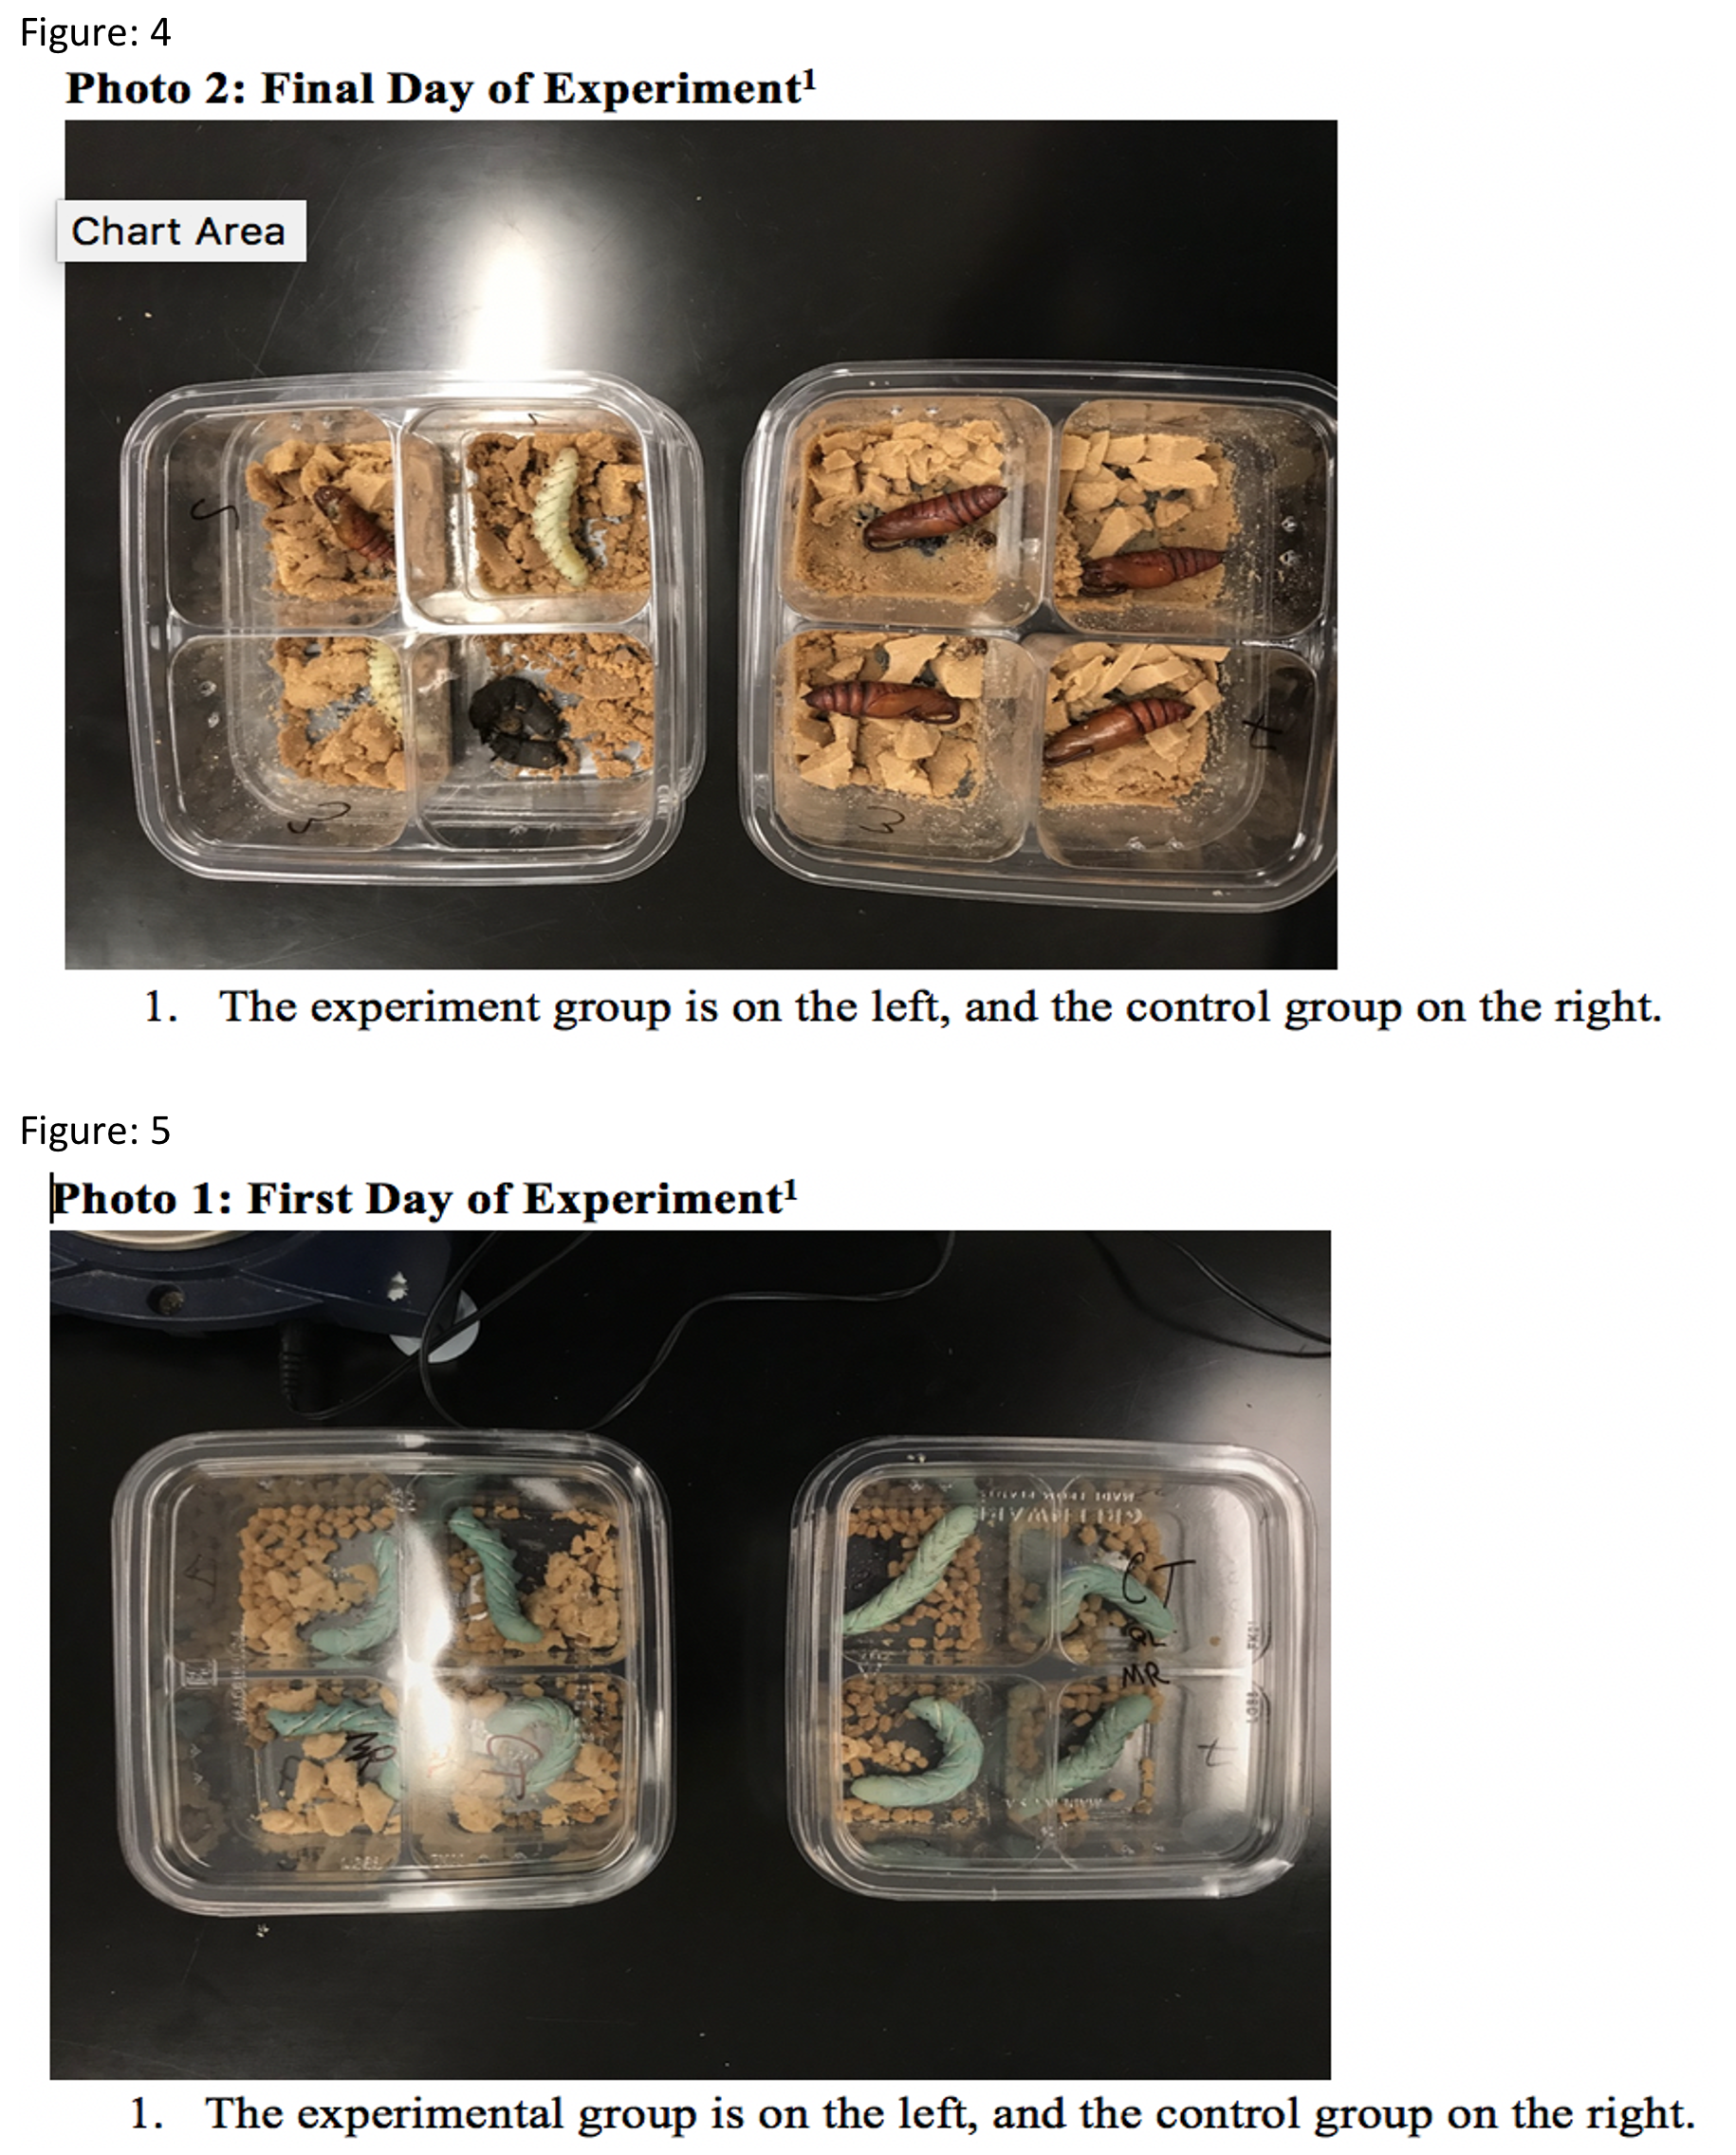
\includegraphics[width=0.8\textwidth,height=\textheight]{images/Manduca_panel.png}
\caption{Photo 1: First Day of Experiment1 1. The experimental group is on the left, and the control group on the right. Photo 2: Final Day of Experiment1 1. The experiment group is on the left, and the control group on the right.}
\end{figure}

\textbf{What Could Be Improved?}

\begin{enumerate}
\def\labelenumi{\arabic{enumi}.}
\tightlist
\item
  The photos are presented out of order. Figure 4 shows the last day of the experiment, and Figure 5 shows the first day.
\item
  The photos have titles with footnotes; all of this text should only be in the legend.
\item
  The caterpillars are photographed on Day 1 with the lids on. The reflection obscures them from view.
\item
  There is no interpretation or explanation of what we are seeing on the final day.
\end{enumerate}

\hypertarget{example-2-12}{%
\subsection{Example 2}\label{example-2-12}}

\begin{figure}
\centering
\includegraphics[width=0.8\textwidth,height=\textheight]{images/Tubes.png}
\caption{Figure 1 shows the difference in color for test tubes 1-3 which had pH 3 buffer, along with the same constants the rest of the tubes had. This photo shows why the procedure deviation was necessary.}
\end{figure}

\textbf{What Could Be Improved?}

\begin{enumerate}
\def\labelenumi{\arabic{enumi}.}
\tightlist
\item
  This photograph probably is not needed. The color difference could have just have been stated in the text.
\item
  The photo is not cropped to remove the extraneous background.
\item
  The legend is not very informative. It says ``\ldots along with the same constants the rest of the tubes had. This photo shows why the procedure deviation was necessary.'' What constants? How does this photo show why the procedure had to be changed?
\end{enumerate}

\hypertarget{example-3-9}{%
\subsection{Example 3}\label{example-3-9}}

\begin{figure}
\centering
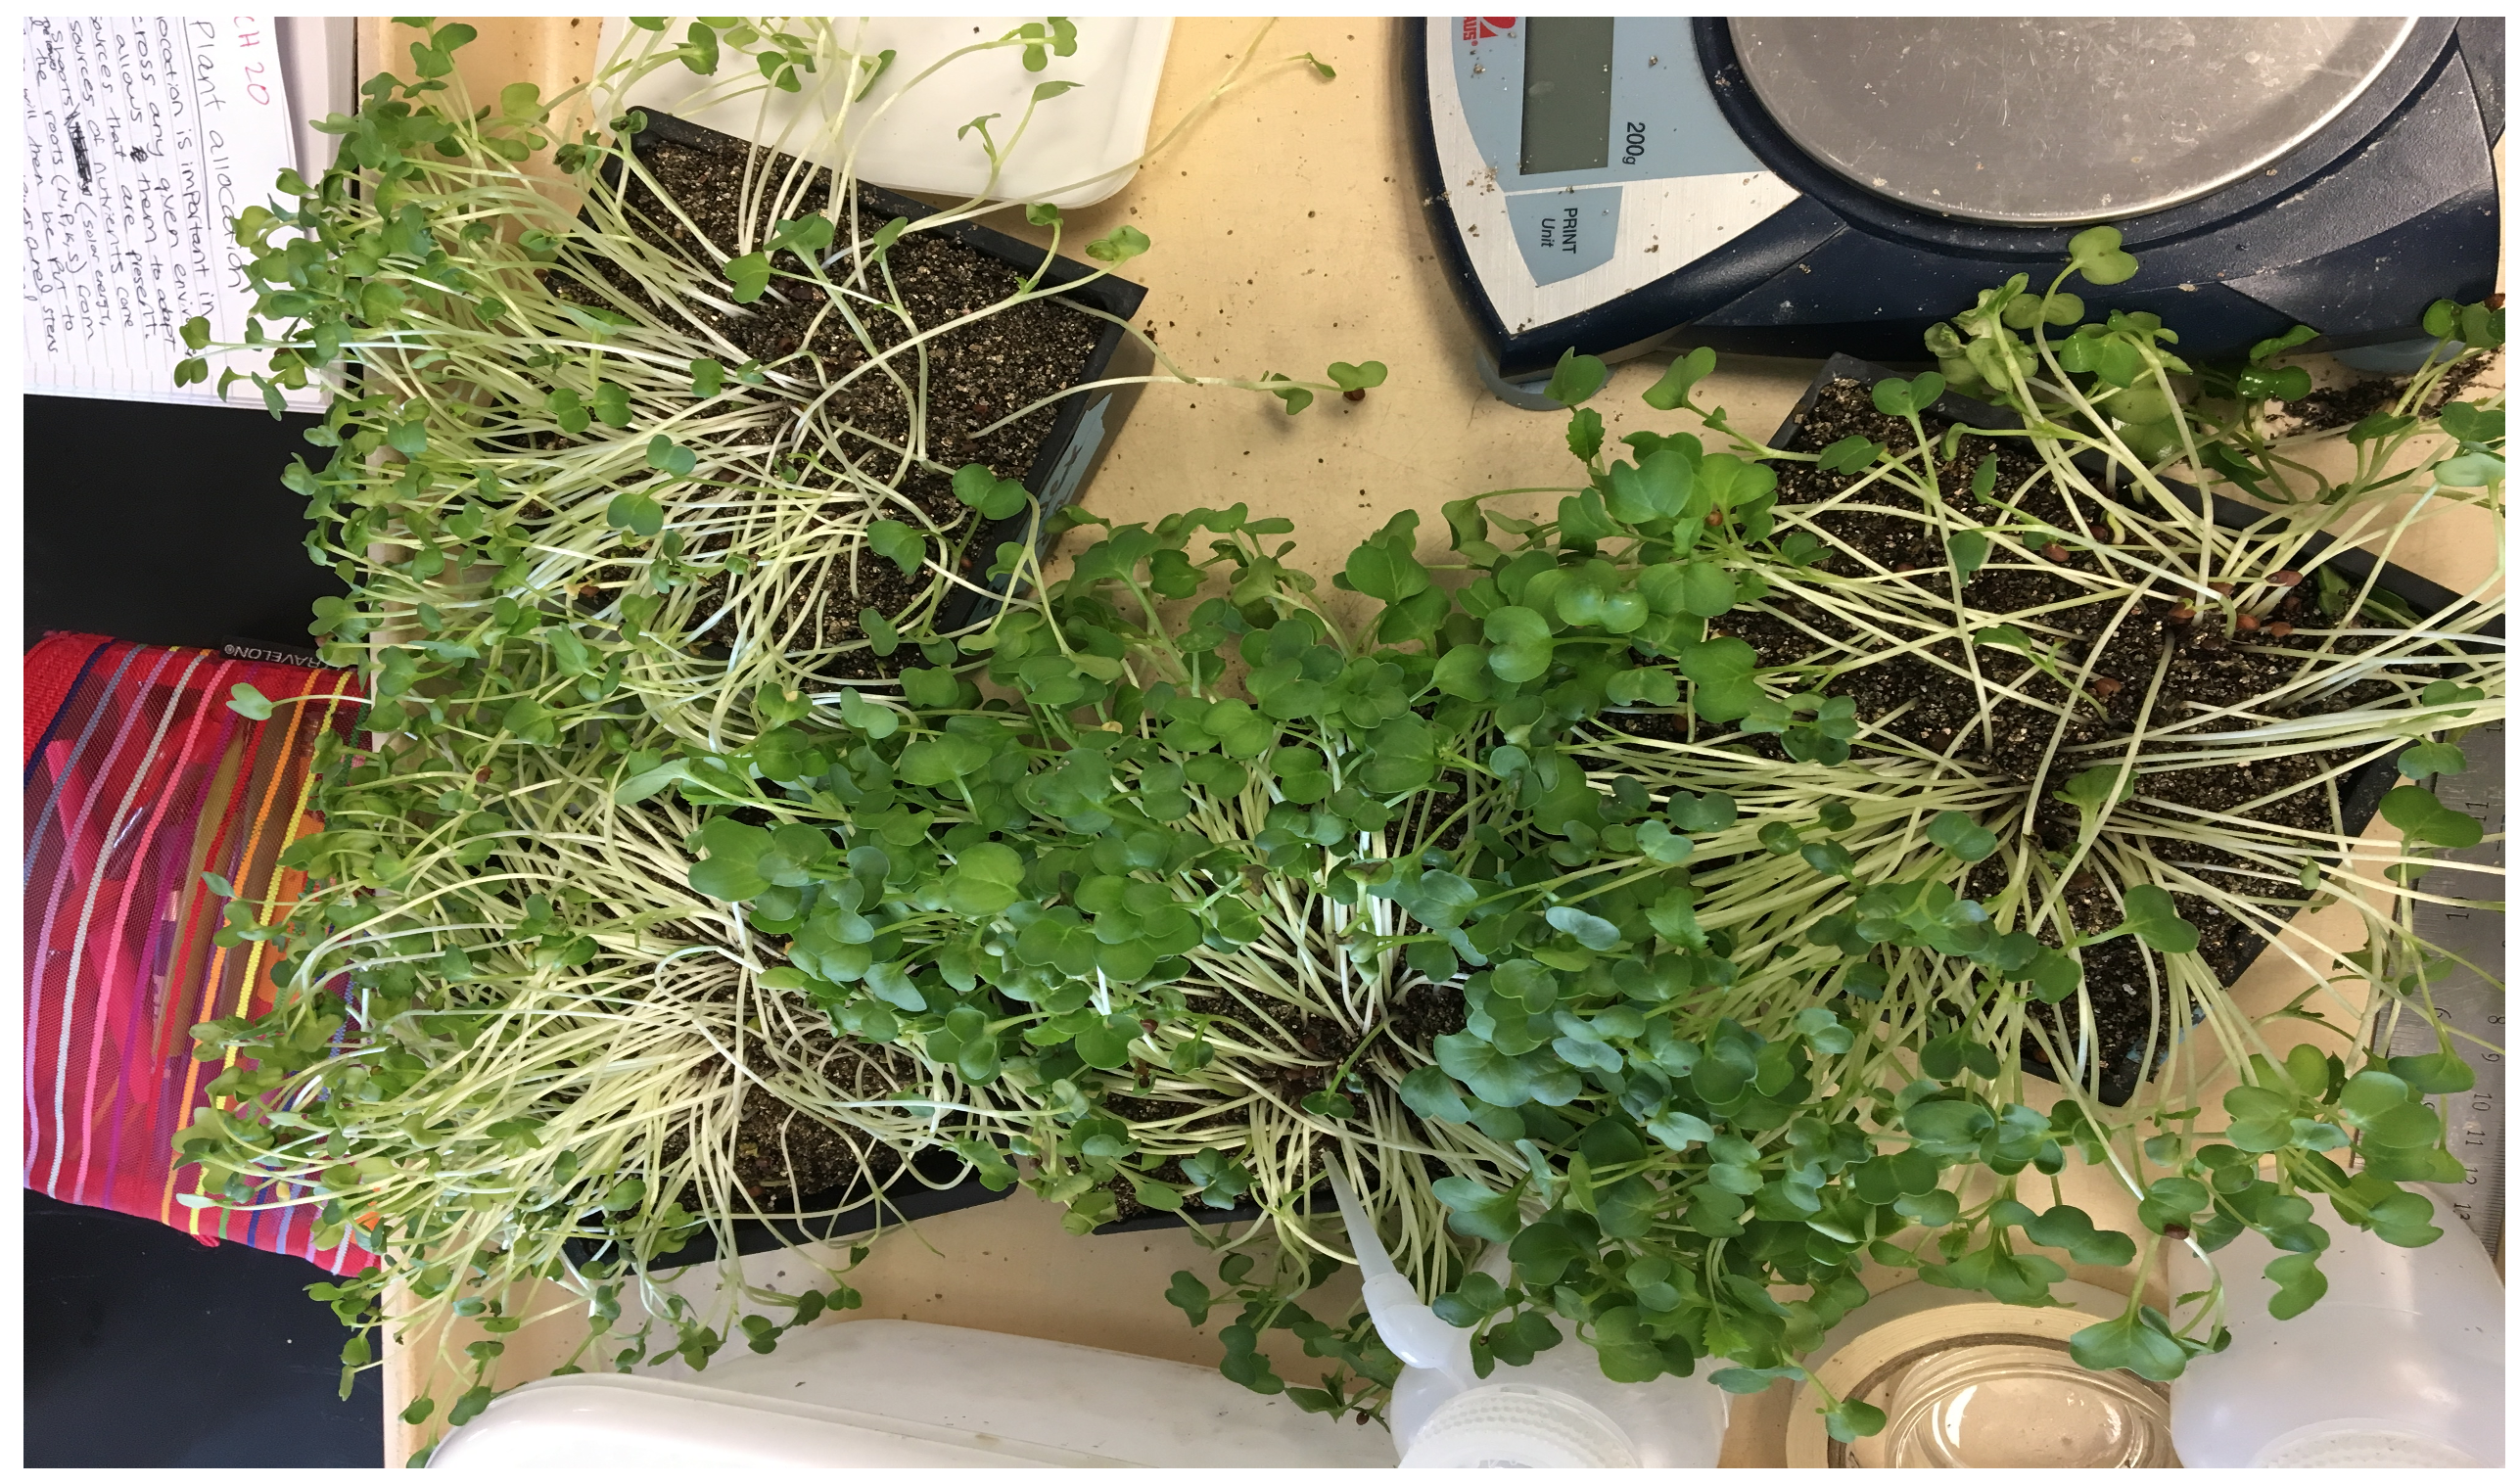
\includegraphics[width=0.8\textwidth,height=\textheight]{images/Cluttered_plants.png}
\caption{Photo 1: Plants grown in light and shade conditions.}
\end{figure}

\textbf{What Could Be Improved?}

\begin{enumerate}
\def\labelenumi{\arabic{enumi}.}
\tightlist
\item
  The background is very cluttered with items that do not have anything to do with the study.
\item
  Which plants were grown in shade, and which ones in light? The legend does not say, so we have to guess.
\item
  What should we notice or pay attention to?
\end{enumerate}

\hypertarget{example-4-3}{%
\subsection{Example 4}\label{example-4-3}}

\begin{figure}
\centering
\includegraphics[width=0.8\textwidth,height=\textheight]{images/Bad_crop.png}
\caption{Figure 1: Root: shoot length ratio in centimeters of non-nitrogen treated and nitrogen treated groups. Error bar denotes standard deviation.}
\end{figure}

\textbf{What Could Be Improved?}

\begin{enumerate}
\def\labelenumi{\arabic{enumi}.}
\tightlist
\item
  This bar graph was inserted as an uncropped screen shot. It needs to be cropped down so only the graph is showing. Better yet, save the graph as a separate image file.
\item
  Remove the figure legend from the photo.
\item
  In the legend, how many observations (``n'') do the mean and s.d. represent?
\end{enumerate}

\hypertarget{examples-of-well-chosen-photos-and-diagrams}{%
\section{Examples of Well-Chosen Photos and Diagrams}\label{examples-of-well-chosen-photos-and-diagrams}}

\hypertarget{example-1-13}{%
\subsection{Example 1}\label{example-1-13}}

\begin{figure}
\centering
\includegraphics[width=0.8\textwidth,height=\textheight]{images/Herbivory.png}
\caption{Figure 1. A. A container of field pea seedlings that are 7 days old, before being treated to simulated herbivory. B. A container of field peas with holes punched in the leaves to simulate herbivory.}
\end{figure}

\textbf{What is Particularly Good?}

\begin{enumerate}
\def\labelenumi{\arabic{enumi}.}
\tightlist
\item
  The images are cropped so only the important details are showing.
\item
  The photos are taken far enough from the containers to see the range of control and treatments plants.
\end{enumerate}

\hypertarget{example-2-13}{%
\subsection{Example 2}\label{example-2-13}}

\begin{figure}
\centering
\includegraphics[width=0.8\textwidth,height=\textheight]{images/Murky_water.png}
\caption{Figure 1. Comparison of betta visibility in clear water (left, control) and murky water (right, experimental). Compare the relative colors of the same fish in the two conditions, and how clearly the room beyond the tank shows through.}
\end{figure}

\textbf{What is Particularly Good?}

\begin{enumerate}
\def\labelenumi{\arabic{enumi}.}
\tightlist
\item
  The image is cropped so that the two most important features (colors of the fish, and clarity of the room beyond) are highlighted, and all extraneous parts of the image have been removed.
\item
  The legend makes it clear what the reader should take away.
\end{enumerate}

\hypertarget{example-3-10}{%
\subsection{Example 3}\label{example-3-10}}

\begin{figure}
\centering
\includegraphics[width=0.8\textwidth,height=\textheight]{images/Four_myograms.png}
\caption{Example of a myogram collected after a frog leg was injected with A23187 calcium ionophore. Each myogram has a higher peak amplitude than the previous one.}
\end{figure}

This diagram is an unusual case. At first it looks like the author has included raw data, but the figure legend explains that they are trying to illustrate one of their observations from the experiment. In this instance, including one example of raw data from their dataset was appropriate.

\hypertarget{tables435}{%
\chapter{Summarizing Data: Data Tables}\label{tables435}}

Students sometimes get confused when we say tables, and it is partly our fault, because there are TWO kinds. \textbf{Data collection tables} are what you use to collect and organize raw data as you conduct an experiment. Your data collection tables are drawn in a paper-based lab notebook, entered in an electronic lab notebook, or created using MS Excel or Word. These tables contain unedited information that is meant for your use. You may be asked to turn in data collection tables as part of a class assignment. However a lab report should never contain raw unanalyzed data.

\textbf{Data summary tables} bring together the raw data points, summarize them in some way, and present the summary values or information so that another reader can make sense of the data quickly. All of the data tables in a lab report should present summarized data.

\begin{figure}
\centering
\includegraphics[width=0.8\textwidth,height=\textheight]{images/Table-annotated.png}
\caption{\textbf{Anatomy of a well-formatted data summary table}. This example shows both a title with footnotes, and a full legend. In practice, a table will have \textbf{either} a short 1-line title above the table plus a few short footnotes, \textbf{or} a longer table legend that goes below the table itself. We only show table titles because you may see them in articles you read. For your lab reports, do not use a table title and footnotes; use a table legend.}
\end{figure}

Each table should have a Table \# and should be numbered in the order they are referred to in your text. You MUST reference each table in the text of your lab report. If you do not reference each table, readers do not know where to look for the data you are using to support your claims.

Data summary tables should have neatly arranged rows and columns, and the data should be easy to read (not crowded). Clearly label the columns and rows of your table. Keep the column titles short. If longer titles cannot be avoided, use 1-2 word column titles in the table, then explain the column titles further in the table legend.

The description of the table goes in the table legend. The table legend is like a figure legend in it explains details of the table that had to be left out to maximize legibility, and helps the reader interpret the table correctly.

Specific points of reference in the table can be either numbered with a superscript or marked with symbols like ``*``,''†``, or''‡'' then explained in detail in the table legend.

Beyond these basic guidelines, there are innumerable ways to organize data summary tables. As you read scientific articles, pay attention to how they lay out their tables. Which ones make it easier to understand their argument or review their evidence? Those are the tables you SHOULD use as models. Which tables are hard to understand? Why? Those are examples of what you should NOT do.

\hypertarget{creating-more-effective-tables}{%
\section{Creating More Effective Tables}\label{creating-more-effective-tables}}

These tips address the most frequent mistakes we see in our students' summary tables.

\begin{itemize}
\tightlist
\item
  DO NOT make a table with all of your raw data observations.
\item
  Be sure your tables are legible. Do not try to put too much data in a single table. Crowded tables are hard to interpret.
\item
  The numbers are the most important part of the table. Make sure they are the most prominent element of the table.
\item
  Use the minimum amount of text you can.
\item
  Present information in a table or a graph, not both.
\end{itemize}

\hypertarget{examples-of-poorly-made-data-tables}{%
\section{Examples of Poorly Made Data Tables}\label{examples-of-poorly-made-data-tables}}

\hypertarget{example-1-14}{%
\subsection{Example 1}\label{example-1-14}}

\includegraphics{images/Raw_data1.png}

\textbf{What Could Be Improved?}

\begin{enumerate}
\def\labelenumi{\arabic{enumi}.}
\tightlist
\item
  This table presents the raw observations the author made. Averaging the weights over the 7 days does not change the fact this is raw data.
\item
  The table is misleading. It does not actually describe the caterpillars' weight \textbf{gain}, just the average weight over 7 days.
\item
  The legend does not say what the experimental group has been treated with.
\item
  The legend calls this a figure, when it is a table.
\end{enumerate}

\hypertarget{example-2-14}{%
\subsection{Example 2}\label{example-2-14}}

\begin{figure}
\centering
\includegraphics{images/Methods_table.png}
\caption{\textbf{Table 2}. The reagents used to prepare control plates (1-3) and the test plates (4-6).}
\end{figure}

\textbf{What Could Be Improved?}

We see tables like this one fairly often. The author is using a table to explain their methods. This is not bad on its own, but look at how much information is repeated. The table could easily be reduced to 3 columns: Reagents, Plates 1-3, and Plates 4-6. Or, the table could be eliminated entirely and this description included in the text of the Methods section.

\hypertarget{example-3-11}{%
\subsection{Example 3}\label{example-3-11}}

\begin{figure}
\centering
\includegraphics{images/Raw_data2.png}
\caption{\textbf{Table 3}. Daily mass measurement of Manduca sexta. ``Control \#'' refers to the control group that wasn't exposed to a 20E inhibitor, ``Expm \#'' refers to the experimental group that was treated with the 20E inhibitor (AzaGuard). Values are weights in grams.}
\end{figure}

\textbf{What Could Be Improved?}

At first this looks like a very informative table. However it has several things that need to be corrected.

\begin{enumerate}
\def\labelenumi{\arabic{enumi}.}
\tightlist
\item
  The table contains raw, unsummarized data.
\item
  The dark fill colors make it hard to read the values in the table.
\item
  Why is ``Pupation Period'' defined in the legend? Where is that used?
\item
  It would be better as a figure, not a table.
\end{enumerate}

\hypertarget{examples-of-well-made-data-tables}{%
\section{Examples of Well-Made Data Tables}\label{examples-of-well-made-data-tables}}

\hypertarget{example-1-15}{%
\subsection{Example 1}\label{example-1-15}}

\begin{figure}
\centering
\includegraphics{images/Good_table1.png}
\caption{\textbf{Table 4}. Average DCIP absorbance when mixed with spinach chloroplasts at different pHs. Means and standard deviations are for n=7 independent replicate samples.}
\end{figure}

\textbf{What is Particularly Good?}

These data should have been presented in a graph, but the author chose to present them as a table. Otherwise it is a well-designed table.

\begin{enumerate}
\def\labelenumi{\arabic{enumi}.}
\tightlist
\item
  The average values are lined up so we can make direct comparisons easily. If we go down a column, we can see the trends at each time point.
\item
  The vertical lines create a clear separation between the data at the different time points.
\item
  The table caption explains the conditions under which the data were collected, and what the summary statistics represent.
\item
  There is enough white space to make the numbers easy to read.
\end{enumerate}

\hypertarget{example-2-15}{%
\subsection{Example 2}\label{example-2-15}}

\begin{figure}
\centering
\includegraphics{images/Good_table2.png}
\caption{\textbf{Table 5}. Difference in average DCIP absorbance when mixed with spinach chloroplasts at different pHs. Values are percent change in absorbance from time zero. Means and standard deviations are for n=7 independent replicate samples. Changes in percent absorbance at pH 9 vs.~11 for each time point were compared using a two-sample t-test. p-values for each time point are shown next to the observed means.}
\end{figure}

\textbf{What is Particularly Good?}

Like the previous example, this table summarizes some of the numerical data, and also includes the results of the comparison statistics.

\begin{enumerate}
\def\labelenumi{\arabic{enumi}.}
\tightlist
\item
  It is clear from the legend what the percent change represents.
\item
  The numbers are arranged so it is clear which numbers represent which subsets of the data.
\item
  The table legend does not interpret the observations, only reports them.
\end{enumerate}

\hypertarget{example-3-12}{%
\subsection{Example 3}\label{example-3-12}}

This example began with the same data as Example 3 in the group of poor tables. We have reorganized and reformatted the same data so it is more informative and better presented. We also revised the figure legend.

\begin{figure}
\centering
\includegraphics{images/Good_table3.png}
\caption{\textbf{Table 6}. Daily weight gain of \emph{Manduca sexta} fed control diet vs.~diet amended with AzaGard. Daily weights are reported as means for the 4 replicate animals in the control and experimental groups. Weight change from day zero was calculated separately for each animal by subtracting its initial weight from the current day's weight, dividing by initial weight, then averaging the values for the 4 replicates. ``Break'' indicates a gap in daily data collection when the labs were closed due to severe weather. Results of the statistical comparison of the control and treatment group are in the main text of the Results section.}
\end{figure}

\textbf{What is Particularly Good?}

\begin{enumerate}
\def\labelenumi{\arabic{enumi}.}
\tightlist
\item
  The table still shows the changes in weights over time, but only as summarized data (means and standard deviations). Readers can see more easily that, on average, control caterpillars reached an average of 8.95g at peak weight, while AzaGard treated caterpillars reached a lower peak weight of 6.28g.
\item
  The table adds a second data series that shows the \textbf{change} in weights relative to Day Zero. This makes it easier for a reader to see that, by Day 3, control caterpillars had increased their weight by 126\% over baseline, but AzaGard-treated caterpillars only increased their weight by 60\% over baseline.
\item
  The table legend says clearly where the reader can find the statistical comparisons between the groups.
\item
  They have not tried to hide the gap in the time series. They point out where there is a gap, and briefly say why.
\item
  The color coding has been removed entirely. That information was moved into the main text.
\end{enumerate}

\hypertarget{instructors-supplement-4}{%
\section{Instructors' Supplement}\label{instructors-supplement-4}}

\hypertarget{rationale-1}{%
\subsection{Rationale}\label{rationale-1}}

We have had endless arguments with GTAs and other faculty about the appropriate formats for figures and tables. Should there be a title above each table and figure, or not? Should a table have a legend below it? What information goes where?

We decided to follow one consistent format so as not to confuse students. Both tables and figures are expected to have a legend immediately below them (not on a separate page), starting with the number of the table or figure. The legends should be sufficiently descriptive for the reader to be able to understand the key points of the table or figure without having to refer to the text.

Alternatively, a table can have a SHORT title above it and brief footnotes below. We do not recommend students use this format, but we do not count off for it given that it is what students see in published literature. If a student uses this alternative format, it should be used consistently for all tables; it is not acceptable for figures.

\hypertarget{adapting-your-guide-3}{%
\subsection{Adapting Your Guide}\label{adapting-your-guide-3}}

Identify the 5-7 most frequent errors that you or your instructors see in students' tables. Then revise the list under ``Creating More Effective Tables'' accordingly. Also, replace our examples of poor vs.~good tables with examples that reflect your own expectations.

\hypertarget{biostats450}{%
\chapter{Summarizing and Analyzing Your Data With Statistics}\label{biostats450}}

You will be using a variety of statistical tests to evaluate your data. These tests quantify the probability that you have obtained your results by chance, which lets you to determine whether you should accept or reject your hypothesis.

Tables 1-3 below outline the most common statistical methods used in general biology teaching labs. Each tool or test is explained in more detail on subsequent pages of the Guide with a:

\begin{itemize}
\tightlist
\item
  Description of what the test is used for;
\item
  What the statistical hypotheses should look like;
\item
  Sample of the test applied to a small dataset; and
\item
  Description of how to interpret and report your data.
\end{itemize}

\textbf{Table 1.} Descriptive and Summary Statistics

\begin{longtable}[]{@{}
  >{\raggedright\arraybackslash}p{(\columnwidth - 4\tabcolsep) * \real{0.3333}}
  >{\raggedright\arraybackslash}p{(\columnwidth - 4\tabcolsep) * \real{0.3333}}
  >{\raggedright\arraybackslash}p{(\columnwidth - 4\tabcolsep) * \real{0.3333}}@{}}
\toprule
\begin{minipage}[b]{\linewidth}\raggedright
Tool or Test
\end{minipage} & \begin{minipage}[b]{\linewidth}\raggedright
Example
\end{minipage} & \begin{minipage}[b]{\linewidth}\raggedright
How Is It Used?
\end{minipage} \\
\midrule
\endhead
Arithmetic Mean & 2019 mean household income in the US was \$116,735. & Estimates the middle of the range of values mathematically. \\
Median & 2019 median household income in the US was \$68,703 & Estimates the middle of a range of values using observed measures. Measurements are sorted in rank order; the middle measurement is the estimated middle of the distribution. \\
Standard Deviation & example & Estimated spread in the measurements \\
\bottomrule
\end{longtable}

\textbf{Table 2.} Comparisons and Hypothesis Testing

\begin{longtable}[]{@{}
  >{\raggedright\arraybackslash}p{(\columnwidth - 4\tabcolsep) * \real{0.3333}}
  >{\raggedright\arraybackslash}p{(\columnwidth - 4\tabcolsep) * \real{0.3333}}
  >{\raggedright\arraybackslash}p{(\columnwidth - 4\tabcolsep) * \real{0.3333}}@{}}
\toprule
\begin{minipage}[b]{\linewidth}\raggedright
Tool or Test
\end{minipage} & \begin{minipage}[b]{\linewidth}\raggedright
Example
\end{minipage} & \begin{minipage}[b]{\linewidth}\raggedright
How Is It Used?
\end{minipage} \\
\midrule
\endhead
Two-sample t-test & Comparing the mean heavy metal content of clams collected in Nova Scotia vs.~New Jersey & Tests a null hypothesis that the means of a measurement variable are the same in two groups. \\
Paired t-test & Compare cholesterol level in blood of people before vs.~after switching to a vegetarian diet. & Tests a null hypothesis that the means of the measurement variable are the same before vs.~after a treatment. \\
ANOVA & Compare blood cholesterol levels of male vegetarian, female vegetarian, male omnivorous, and female omnivorous students. & Tests a null hypothesis that 3+ different groups have the same means for the measurement variable. \\
Chi-square goodness of fit & The number of red, pink, white flowers in a genetic cross fits an expected 1:2:1 ratio & Tests a null hypothesis that observed frequencies are not different from expected frequencies. \\
Chi-square independence & Compare the proportion of HIV patients who get worse after taking a new drug to the proportion who get worse after taking a placebo & Tests a null hypothesis that proportions are same in different groups. \\
\bottomrule
\end{longtable}

\textbf{Table 3.} Statistical Modeling

\begin{longtable}[]{@{}
  >{\raggedright\arraybackslash}p{(\columnwidth - 4\tabcolsep) * \real{0.3333}}
  >{\raggedright\arraybackslash}p{(\columnwidth - 4\tabcolsep) * \real{0.3333}}
  >{\raggedright\arraybackslash}p{(\columnwidth - 4\tabcolsep) * \real{0.3333}}@{}}
\toprule
\begin{minipage}[b]{\linewidth}\raggedright
Tool or Test
\end{minipage} & \begin{minipage}[b]{\linewidth}\raggedright
Example
\end{minipage} & \begin{minipage}[b]{\linewidth}\raggedright
How Is It Used?
\end{minipage} \\
\midrule
\endhead
Correlation & Measure salt and fat intake in different people's diets, to see if people who eat a lot of fat also eat a lot of salt & See whether two variables are \textbf{potentially} related to each other. (Correlation is not the same as a causal relationship.) \\
Linear regression & Measure chirping speed in crickets at different temperatures, \& test whether chirping speed varies with temperature & See if changes in an independent variable predict changes in a dependent variable. \\
" & Estimate air temperature based on chirping speed of crickets & Estimate the value of one unmeasured variable corresponding to a measured variable \\
\bottomrule
\end{longtable}

\hypertarget{where-to-learn-more-3}{%
\section{Where to Learn More}\label{where-to-learn-more-3}}

This Guide covers just a fraction of all there is to know about biostatistics. This introduction will get you started thinking about some foundation concepts and using some simple tests. When you are ready, check out these additional resources.

\href{https://www.biointeractive.org/classroom-resources/data-explorer}{HHMI Data Explorer} is an interactive web site that you can use to build graphs and learn how different parts go together. In the \textbf{Materials} box on the right side is a link to download the \textbf{HHMI Statistical Analysis Selection Guide}. This short reference helps you choose the right statistical test for your data.

\emph{MacDonald's Biostatistics Handbook}. This is an exceptional resource. Much of the information in this portion of the Guide is based on Dr.~MacDonald's book, which he kindly granted us permission to use. \url{http://www.biostathandbook.com/}

Motulsky H. 2013. \emph{Intuitive Biostatistics: A Non-Mathematical Guide to Statistical Thinking,} 3rd edition. Oxford University Press, 576 pp.~

Nuzzo R. 2014. Statistical errors: P values, the `gold standard' of statistical validity, are not as reliable as many scientists assume. \emph{Nature}, 506:150-152.

\hypertarget{instructors-supplement-5}{%
\section{Instructors' Supplement}\label{instructors-supplement-5}}

\hypertarget{adapting-your-guide-4}{%
\subsection{Adapting Your Guide}\label{adapting-your-guide-4}}

Our introduction to biostatistics describes the statistical tests that our students use most often. If there are other statistical tests that are more appropriate for the types of analyses your students do, add new descriptions for them to the tables on this page, add new pages outlining each test, and remove any current ones that are not needed.

Alternatively, if your students have a separate statistics resource guide, the pages on biostatistics in this guide should be deleted entirely.

\hypertarget{sumstats460}{%
\chapter{Biostatistics 1: Summary Statistics}\label{sumstats460}}

Summary statistics make it much easier for your readers to understand and think about your data. The questions you want to answer for your readers are:

\begin{itemize}
\tightlist
\item
  What is the midpoint of your observed data?
\item
  How wide is the range of your observed data?
\item
  Are your observed data points similar to each other, or spread far apart?
\end{itemize}

Mean and median values provide them with estimates of the midpoints of each of your experimental groups. Standard deviation, standard error, variance, etc. (what we call \textbf{measures of dispersion}) provide readers with an estimate of the range or spread of your data, and how the measurements are distributed.

For these statistics to make sense we need to explain what we mean by distributions.

\hypertarget{normal-distribution}{%
\section{Normal Distribution}\label{normal-distribution}}

Statistics is built around assumptions about how data are distributed. Imagine we measured the height of every student on campus. We get the following data set.

\textbf{Table 1.} Distribution of student height on campus.

\begin{longtable}[]{@{}cc@{}}
\toprule
Height (cm) & \# students \\
\midrule
\endhead
\textless135 (4'5'') & 44 \\
135-139 & 109 \\
140-149 & 231 \\
150-159 & 536 \\
160-169 & 984 \\
170-179 (5'10'') & 2016 \\
180-189 & 1051 \\
190-199 & 486 \\
200-209 & 194 \\
210-219 & 85 \\
\textgreater219 (7'2'') & 52 \\
Total & 5788 \\
\bottomrule
\end{longtable}

If we plot these data as a series of bars showing the counts for each category, we get a \textbf{histogram} like the one in Figure 1.

\begin{figure}
\centering
\includegraphics[width=0.8\textwidth,height=\textheight]{images/Histogram1.png}
\caption{\textbf{Figure 1.} Histogram showing the distribution of student height on campus.}
\end{figure}

The histogram shows us the \textbf{distribution} of the numbers that represent our observations. The histogram shows there are about the same number of students on either side of the peak (there are 1904 students who are less than 170 cm tall, and 1868 students who are greater than 179 cm tall.) Data are said to have a \textbf{normal distribution} when there are about the same number of data points above and below the midpoint.

Suppose we observed instead that there are 2744 students who are less than 170 cm tall, and 1028 students who are greater than 179 cm tall. The midpoint of the data still is 170-179 cm, but now the data are not normally distributed. We call this a \textbf{skewed distribution}.

\begin{figure}
\centering
\includegraphics[width=0.8\textwidth,height=\textheight]{images/Histogram2.png}
\caption{\textbf{Figure 2.} Histogram showing a skewed distribution of student height on campus. The blue bars show the normal distribution from Figure 1. The orange bars are the skewed distribution.}
\end{figure}

When writing up your own experiments in lab reports, you will be working with smaller datasets, and skewed distributions will not be a big concern. When you begin working with larger datasets, there are statistical methods for quantifying the relative amount of skew in the data distributions.

\hypertarget{arithmetic-mean}{%
\section{Arithmetic Mean}\label{arithmetic-mean}}

There are many ways to describe the midpoint of your summarized data but most of the time you will be describing your data using an arithmetic mean.

The \textbf{arithmetic mean (x̅)}, or simply the \textbf{mean} is the sum of all the observations divided by the number of observations. It is the most common statistic that describes data that is symmetrically distributed in a frequency graph. When someone says ``the mean'' or ``the average,'' this is what they are talking about.

For example, the counts in each of the bins in Table 1 add up to 5788. The arithmetic mean is:

\begin{quote}
x̅ = 5788 (sum of all observations)/11 (\# bins) = 526.2 students/bin
\end{quote}

Arithmetic mean is very useful, but also sensitive to extreme values, which means it does not work well for data that are highly skewed. Imagine that you are measuring the heights of trees in two areas of equal size.

\begin{figure}
\centering
\includegraphics[width=0.8\textwidth,height=\textheight]{images/Tree-plots.png}
\caption{\textbf{Figure 3}. Two forest plots.}
\end{figure}

Plot A is in a mature, undisturbed forest. Plot B experienced a fire a few years ago that killed all but 2 very large trees. Since then, new seedlings have sprouted. There are dozens of small trees now, all about the same height.

If we calculate the arithmetic mean of the tree heights in the two plots, we might calculate that the mean tree height is similar for the two plots even if our eyes tell us that is not right. So the arithmetic mean alone does not provide enough information to compare the plots. We need to report a second value that describes the dispersion of the data points.

\hypertarget{advanced-topic-other-ways-to-calculate-means}{%
\subsection{Advanced Topic: Other Ways to Calculate Means}\label{advanced-topic-other-ways-to-calculate-means}}

You will not use them in most biology classes, but there are many other ways to estimate the mean for a set of measurements. The \textbf{geometric mean} is often used to describe the mid-point of numbers that grow exponentially. For example, human population growth rate has grown exponentially over time. If we wanted to express the mean value, we would use the geometric mean. The other mean used in science regularly is the \textbf{harmonic mean}, which is used to describe the mid-point for ratios or rates like speed.

These and other ways to calculate means are useful in particular situations. When you are first starting out in biostatistics, it is safer to stick with a simple arithmetic mean. As specific situations arise, your instructor may introduce other ways to calculate means.

\hypertarget{advanced-topic-median}{%
\section{Advanced Topic: Median}\label{advanced-topic-median}}

Where the mean is a mathematical descriptor of your data, the \textbf{median} estimates the middle of the distribution is the actually \textbf{observed} middle of a range of observed values. We determine median by sorting the values in rank order (lowest to highest). The median is the middle measurement in the set.

For example, these are the counts in each of the bins in Table 1, sorting in order: 44, 52, 85, 109, 194, 231, 486, 536, 984, 1051, 2016. The middle value is the 6th out of the 11 values, or 231. When there are an even number of values, the median is the arithmetic mean of the middle two values.

Median would be included in a report like this:

\begin{quote}
Median = 231, n = 11.
\end{quote}

Median is not very useful when you are working with small datasets. It is more informative when you have dozens to hundreds of data points. We point it out here mainly so you do not confuse it with mean.

\hypertarget{standard-deviation}{%
\section{Standard Deviation}\label{standard-deviation}}

For routine lab work you mostly will use standard deviation to describe the dispersion of your data points.

\textbf{Standard deviation (SD)} is a measure of the spread of data points in a distribution around the mean, using the same units as the data points in that distribution. It measures how far from the mean observations typically are. When the standard deviation is large compared to the mean, that tells us most observations are far from the mean. Conversely, if the standard deviation is small, most measurements lie close to the mean.

Standard deviation has a predictable relationship to the normal distribution. When data are normally distributed:

\begin{itemize}
\tightlist
\item
  68\% of data points within a dataset will have values within ±1 standard deviation of the mean
\item
  95\% of data points within a dataset will have values within ±2 standard deviations of the mean
\item
  99.7\% of data points within a dataset will have values within ±3 standard deviations of the mean.
\end{itemize}

Standard deviation is directly correlated to the number of measurements. The more measurements you use to calculate standard deviation, the smaller the value will be. So when we report standard deviation, we always report the number of observations (n) used to calculate it.

\hypertarget{calculating-summary-statistics-in-excel}{%
\section{Calculating Summary Statistics in Excel}\label{calculating-summary-statistics-in-excel}}

You can use MS Excel to calculate mean and standard deviations for numerical measurements.

\begin{itemize}
\tightlist
\item
  Use the formula ``=AVERAGE(\url{data:range})'' to calculate the arithmetic mean for all values in the cells listed in ``\url{data:range}''.
\item
  Use ``=STDEV(\url{data:range})'' to calculate the standard deviation.
\end{itemize}

\hypertarget{reporting-mean-standard-deviation-and-observations}{%
\section{Reporting Mean, Standard Deviation, and \# Observations}\label{reporting-mean-standard-deviation-and-observations}}

In the text of a report, you should always report summary statistics as mean, standard deviation, and number of measurements (x-bar, s or s.d., and n). For example, we could summarize Table 1 like this:

\begin{quote}
The number of students in each of the height measurement bins ranged from 44 students in the smallest bin to 2016 in the largest bin (x̅ = 526.1 students/bin, s.d.= 61.1, n=11 bins).
\end{quote}

When you are graphing summarized data, you should include error bars representing one standard deviation on the graph itself. The figure legend should state clearly that the error bars represent 1 s.d., and you should include and explain the value for n.~

\hypertarget{compstatsone470}{%
\chapter{Biostatistics 2: Comparing Groups - T-Tests}\label{compstatsone470}}

T-tests are a family of statistical tests that compare two groups of data points to determine whether the means of the measurement variable are the same. All of the tests in the t-test family use the t-distribution to estimate probabilities. The main differences between the various t-tests is what and how the groups are compared.

The most common version is the \textbf{two-sample t-test.} It tests a null hypothesis that the means of a measurement variable are the same in two independently sampled groups.

The other widely used version is a \textbf{paired t-test.} It tests a null hypothesis that the means of the measurement variable are the same before vs.~after a treatment. This test takes into account the pre-existing variation in the measured variable.

This video is a good introduction to \href{https://youtu.be/AGh66ZPpOSQ}{T-tests}

\hypertarget{two-sample-t-tests}{%
\section{Two Sample T-Tests}\label{two-sample-t-tests}}

Two-sample t-tests compare the means from two groups of data. Usually the comparison is between the mean of a control group and the mean of an experimental group. Sometimes though, the comparison is between two experimental groups.

You can use the two-sample t--test when you have one categorical variable and one measurement variable, and you want to compare the mean values of the measurement variable. The categorical variable must have only two values, such as ``present'' and ``absent'' or ``treated'' and ``untreated.''

Two-sample t-tests should only be used when you are comparing data collected from two \textbf{independent groups}. This mean that the data were collected from completely different groups of organisms, different locations, etc. If the groups are connected (paired) you need to use a paired t-test, which is explained in the next section.

There are two versions of the two-sample t-test:

\begin{itemize}
\tightlist
\item
  You should use \textbf{Student's t-test} when the data points in BOTH groups are randomly distributed, not skewed.
\item
  You should use \textbf{Welch's t-test} (also called Welch's unequal variances test) when the measured variables are not equally distributed, or the two groups have different sample sizes.
\end{itemize}

A rule of thumb is that you should use Welch's t-test if either the standard deviations of the two groups you want to compare are more than 10\% different from one another, or the number of observations are more than 10\% different between the two groups.

In practice, the number of data points you usually work with in a biology lab course is small enough that the choice of test is not critical. So if you do not have access to a program that can run Welch's t-test, use Student's t-test.

\begin{quote}
Advanced: There is a long-running debate over which test to use. Some statistics specialists say you should ALWAYS use Welch's t-test, but others say you will overlook small but significant differences. Google ``Welch's vs.~Student's t-test'' if you want to see the arguments on both sides.
\end{quote}

\hypertarget{an-example-of-a-two-sample-t-test}{%
\subsection{An Example of a Two-Sample T-test}\label{an-example-of-a-two-sample-t-test}}

Let's go back to an earlier exploration of the distribution of student height on campus. Now we want to know if there is any difference in average height of students living on the eastern half versus the western half of campus.

\textbf{Table 1.} Distribution of student height on campus.

\begin{longtable}[]{@{}cccc@{}}
\toprule
Height (cm) & \# students, east half & \# students, west half & Total \\
\midrule
\endhead
\textless135 (4'5'') & 24 & 20 & 44 \\
135-139 & 61 & 48 & 109 \\
140-149 & 152 & 79 & 231 \\
150-159 & 269 & 267 & 536 \\
160-169 & 484 & 1015 & 1499 \\
170-179 (5'10'') & 1001 & 672 & 1673 \\
180-189 & 379 & 500 & 879 \\
190-199 & 135 & 351 & 486 \\
200-209 & 62 & 132 & 194 \\
210-219 & 21 & 64 & 85 \\
\textgreater219 (7'2'') & 0 & 52 & 52 \\
Total & 2588 & 3200 & 5788 \\
\bottomrule
\end{longtable}

If we plot these data as a series of bars showing the counts for each category, we see the distribution shown in Figure 1.

\begin{figure}
\centering
\includegraphics[width=0.8\textwidth,height=\textheight]{images/Histogram3.png}
\caption{\textbf{Figure 1.} Histogram showing the distribution of student height on east vs.~west campus. Bars indicate number of students in each height group. Blue bars are students on east campus, orange bars are students on west campus.}
\end{figure}

It looks like there is a difference in the height of students on west vs.~east campus, but can we be sure?

\hypertarget{what-do-the-statistical-hypotheses-look-like-for-a-two-sample-t-test}{%
\subsubsection{What Do the Statistical Hypotheses Look Like For a Two-Sample T-test?}\label{what-do-the-statistical-hypotheses-look-like-for-a-two-sample-t-test}}

The statistical \textbf{null hypothesis (H0)} is that the means of the measurement variable are equal for the two categories.

\begin{quote}
H0: x̅ (Group 1) = x̅ (Group 2)
\end{quote}

In terms of our original question, the null hypothesis is that there is no difference in the height distribution of students living on east (Group 1) vs.~west (Group 2) campus. The differences in bin distributions are due to random chance.

There are two different ways you can describe the \textbf{alternative hypothesis (HA)}. Which way you choose depends on what you know already, or what your predictions are.

If you have some prior information or other observations, you can make a prediction that the two groups will be different from one another in a particular direction. In other words, you can predict in advance which group will have a mean that is significantly greater or less than that of the other group. Depending on the direction you choose, your alternate hypothesis would be:

\begin{quote}
HA: x̅ Group 1 \textgreater{} x̅ Group 2
\end{quote}

\begin{quote}
or
\end{quote}

\begin{quote}
HA: x̅ Group 1 \textless{} x̅ Group 2
\end{quote}

Say you noticed that a lot of taller students live on west campus. So we can choose a hypothesis that includes a specific direction, and predict that the mean height of students living on east (Group 1) campus is less than the mean height of students on west (Group 2) campus. In other words, your alternate hypothesis is HA: x̅ Group 1 \textless{} x̅ Group 2.
Because we have made a prediction of change in one direction in our hypothesis, we will be running a \textbf{one-tailed t-test.}

Now suppose we did not have the histogram in Figure 1. We suspect there is a height difference but we do not have any prior data from which to predict which group will be taller on average. We only can predict that the two groups are different. Now the alternate hypothesis will be:

\begin{quote}
HA: x̅ Group 1 ≠ x̅ Group 2
\end{quote}

Because our hypothesis does NOT predict the direction of change, we would run a \textbf{two-tailed t-test.}

\hypertarget{running-our-experiment}{%
\subsubsection{Running Our Experiment}\label{running-our-experiment}}

To test our hypothesis, we randomly select 100 students (50 from each side of campus), measure their heights, and tabulate the data.

\begin{figure}
\centering
\includegraphics[width=0.5\textwidth,height=\textheight]{images/Height_table1.png}
\caption{\textbf{Table 2.} Measured heights (in cm) of 50 randomly selected students each on east vs.~west campus.}
\end{figure}

\hypertarget{calculating-two-sample-t-tests-in-excel}{%
\subsubsection{Calculating Two-Sample T-Tests in Excel}\label{calculating-two-sample-t-tests-in-excel}}

We will use MS Excel to compare the two sets of measurements. Excel has two ways to calculate the p-value for a two-sample t-test. To obtain the p-value quickly for an informal comparison of two groups, use this formula:

\begin{verbatim}
  =T.TEST(array1,array2,tails,type)
\end{verbatim}

``Arrays 1 and 2'' are the two sets of measured values you want to compare. ``Tails'' is telling Excel to run either a 1- or 2-tailed t-test. ``Type'' is telling Excel what kind of t-test to run: 1 = a paired t-test, 2 = two sample t-test where the two groups have equal variance, and 3 = two sample t-test where the two groups have unequal variance.

The more informative way to calculate a two-sample t-test requires using the Data Analysis package.

\begin{enumerate}
\def\labelenumi{\arabic{enumi}.}
\item
  In the main menu, look under EITHER ``Data'' or ``Tools'' for the option ``Data Analysis. Where this package is located depends on what version of Excel you have and what type of computer you are using.
\item
  Click on Data Analysis to open the dialogue box.
\item
  Select the type of t-test you want to do. For this example we are using a two-sample test assuming equal variance.
\end{enumerate}

\begin{figure}
\centering
\includegraphics[width=0.8\textwidth,height=\textheight]{images/Open_analysis.png}
\caption{\textbf{Figure 2.} The opening dialogue box for Excel's Data Analysis package.}
\end{figure}

\begin{enumerate}
\def\labelenumi{\arabic{enumi}.}
\setcounter{enumi}{3}
\tightlist
\item
  Click and drag the data columns to select the two sets of observations you want to compare. Choose a convenient empty space on the spreadsheet for Excel to print out the results.
\end{enumerate}

\begin{figure}
\centering
\includegraphics[width=0.8\textwidth,height=\textheight]{images/Analysis_dialog.png}
\caption{\textbf{Figure 3.} Selecting the data to be analyzed.}
\end{figure}

\begin{enumerate}
\def\labelenumi{\arabic{enumi}.}
\setcounter{enumi}{4}
\tightlist
\item
  When you click ``OK'' the following data table will be created. It shows you the means for both groups, the degrees of freedom (df), the t-statistic, and the p-values for both a 1-tailed and 2-tailed comparison.
\end{enumerate}

\begin{figure}
\centering
\includegraphics[width=0.8\textwidth,height=\textheight]{images/Analysis_table.png}
\caption{\textbf{Figure 4.} Results of the two-sample t-test. The t-statistic, degrees of freedom, and p-value have been highlighted. When recording the p-value, be careful to pick the right value; p-values for both the one- and two-tailed tests are displayed automatically.}
\end{figure}

\hypertarget{how-to-report-your-t-test-statistics}{%
\subsubsection{How to Report Your T-Test Statistics}\label{how-to-report-your-t-test-statistics}}

When reporting the results of any type of t-test, you should include the t-statistic, the degrees of freedom (df), whether the test was one- or two-tailed, and the corresponding p-value.

Your statement reporting outcomes of this two-sample t-test might look like this:

\begin{quote}
The mean height of students living on west campus was significantly different than mean height of students living on east campus (t-stat = -2.719, df = 98, one-tailed, P = 0.0039).
\end{quote}

The t-statistic (t-stat), degrees of freedom (df), and p-value (P) should all be included when you report the results of a t-test. Though you are unlikely to need them yourself, the t-stat and df are useful to readers because they can calculate additional statistical relationships like confidence intervals for themselves.

\hypertarget{paired-t-test}{%
\section{Paired T-Test}\label{paired-t-test}}

When you have \textbf{pairs of observations} for a group of individuals, organisms, sites, etc., you should compare them using a \textbf{paired t test}. The paired t-test asks whether the mean difference in the pairs is different from 0. The first measurement from each member of the group is the \textbf{control or pre-treatment measurement.} The group is given a treatment or allowed to participate in some event, then you measure each member of the group again; this second measurement is the \textbf{experimental or post-treatment measurement.}

\hypertarget{an-example-of-a-paired-t-test}{%
\subsection{An Example of a Paired T-test}\label{an-example-of-a-paired-t-test}}

Let's change around our campus height example. Suppose that all students live on east campus for their first two years, then move to west campus for the rest of their time in school. Heights of students are measured twice: once in the first year they are living on east campus, then again in their fourth year, after they have moved to west campus.

Now we can ask a different question: do students get taller when they move to west campus?

The null hypothesis (H0) is that student height does not differ across campus.

\begin{quote}
H0: x̄ West campus = x̄ East campus
\end{quote}

Just like the previous t-test, we may have prior observations or a particular reason to predict student height changes in a particular direction. We also can call on common sense: we do not expect young adults to get shorter. So we can state the alternative hypothesis (HA) in the form of a one-tailed t-test.

\begin{quote}
HA: x̅ West campus \textgreater{} x̅ East campus
\end{quote}

If we think there is a difference but we have no data to make a prediction about which direction height changes, we word the alternative hypothesis as a two-tailed test, meaning we expect the means will be significantly different, but cannot predict which direction.

\begin{quote}
HA: x̄ West campus ≠ x̄ East campus
\end{quote}

\hypertarget{running-the-experiment}{%
\subsection{Running the Experiment}\label{running-the-experiment}}

To test our hypothesis, we randomly select 50 students, and tabulate their heights when living on east vs.~west campus.

\begin{figure}
\centering
\includegraphics[width=0.5\textwidth,height=\textheight]{images/Height_table2.png}
\caption{\textbf{Table 3.} Heights (in cm) of 50 randomly selected students, measured in Year 1 when living on east campus, then again in Year 4 when living on west campus.}
\end{figure}

We use the same Excel Data Analysis package described in the two-sample t-test, except this time we choose ``paired t-test.'' The rest of the procedure is the same.

\begin{figure}
\centering
\includegraphics[width=0.8\textwidth,height=\textheight]{images/Paired_T.png}
\caption{\textbf{Figure 5.} Results of the paired t-test. The t-statistic, degrees of freedom, and p-value have been highlighted. If we look at the means for heights of students on west vs.~east campus, we can say that the mean height of students has increased by 3.3 cm. However we cannot say anything about WHY the students are an average of 3.3 cm taller on west campus.}
\end{figure}

\hypertarget{how-to-report-and-interpret-paired-t-test-statistics}{%
\section{How to Report and Interpret Paired T-Test Statistics}\label{how-to-report-and-interpret-paired-t-test-statistics}}

Like the two-sample t-test, your statement of the results should include the t-statistic, the degrees of freedom (df), whether the test was one- or two-tailed, and the corresponding p-value.

Your statement reporting outcomes of a two-sample t-test might look like this:

\begin{quote}
The mean height of students living on west campus was significantly different than mean height of students living on east campus (paired t-test, t-stat = -15.544, df = 49, one-tailed, P = 7.09 x 10-21).
\end{quote}

When you report the results of your statistical tests, be very careful that you do not over-interpret what they mean. For example, when you look at the results of the paired t-test above, which of these interpretations seems right or wrong, and why?

\begin{enumerate}
\def\labelenumi{\arabic{enumi}.}
\tightlist
\item
  ``Based on these results we concluded that moving from east to west campus makes students grow taller.''
\item
  ``These results prove students are taller on west campus.''
\item
  ``These results support the conclusion that mean student height increases between the time students are measured in their first year of school, and their fourth year of school.''
\end{enumerate}

Statement \#1 implies that moving from one side of campus to the other is what \textbf{causes} students to get taller. Simply moving across campus should not do that; something else is going on during that time.

Statement \#2 breaks the basic assumption of statistics (and science): we cannot prove anything is true, we can only provide support for the alternate hypothesis. What if by chance our sample included several members of the basketball team, which lives only on west campus?

Statement \#3 steps back from the east vs.~west campus question, and looks at what is going on biologically BEHIND the scenes. We cannot say the height difference is due to the move, because we did not measure heights just before and just after the move. So the authors stepped back to what they CAN say with certainty. Now they can \textbf{speculate} on what happens between Year 1 and Year 4. It might be:

\begin{itemize}
\tightlist
\item
  Year 1 students are younger, so have not finished growing yet. Most students are going to grow taller between the time they live on east campus and when they move to west campus.
\item
  The football, basketball, and volleyball teams all live on west campus starting their first year. This takes some of the taller people out of the population on east campus. Put another way, the population is naturally skewed.
\item
  The food in the cafeteria on east campus is so bad that students don't eat enough to grow until they move to west campus, where the cafeteria is better.
\end{itemize}

These speculations range from very plausible to very unlikely. Still, they all are testable hypotheses that could be evaluated in future experiments.

\hypertarget{compstatstwo473}{%
\chapter{Biostatistics 3: Comparing Three or More Groups - ANOVA}\label{compstatstwo473}}

Analysis of variance (ANOVA) is an extension of t-tests. It tests whether the means of measurements from three or more treatment groups are equal. It works by comparing whether individuals chosen from different groups are, on average, more different than individuals chosen from the same group.

If your ANOVA test reports a significant p-value, that tells you that \textbf{at least one of the means is different from the other}, but it does not say which treatment groups are different. To compare each pair of groups, we use a \textbf{post-hoc test} like the Tukey-Kramer test. Most post-hoc tests are a modified version of a t-test.

The most common version of ANOVA is the \textbf{one-way ANOVA.} Like a two-sample t-test, it tests a null hypothesis that the means of a measurement variable are the same in three or more independently sampled groups. \textbf{Repeated measures ANOVA} is like the paired t-test, in it tests a null hypothesis that the mean difference in a measured variable between 3+ categorical or treatment groups is zero.

Like t-tests, there are two different versions of ANOVA. Fisher's ANOVA is used when the variance is about the same in all of the groups. Welch's ANOVA is the better choice if there is unequal variance in the groups.

This video is a good introduction to ANOVA: \href{https://youtu.be/oOuu8IBd-yo}{Video Intro to ANOVA}

\hypertarget{an-example-of-one-way-anova}{%
\section{An Example of One-Way ANOVA}\label{an-example-of-one-way-anova}}

There is a disagreement among your friends about the benefits of being a vegetarian. Some say it lowers blood cholesterol (a benefit), while others argue it lowers blood iron levels (which is not good.) You and your friends decide to find out which claim (if either) is true by comparing blood cholesterol and iron levels of male vegetarian (MV), female vegetarian (FV), male omnivorous (MO), and female omnivorous (FO) students.

You have four categories (FO, MO, FV, and MV) that you are comparing for two measurement variables (cholesterol, iron). How do you put the data in a form you can evaluate using ANOVA?

\hypertarget{what-do-the-statistical-hypotheses-look-like-for-one-way-anova}{%
\section{What Do the Statistical Hypotheses Look Like For One-Way ANOVA?}\label{what-do-the-statistical-hypotheses-look-like-for-one-way-anova}}

The null hypothesis is that the population means are the same for all groups. We can state it mathematically as:

\begin{quote}
H0: x̅MV = x̅FV = x̅MO = x̅FO
\end{quote}

The alternative hypothesis is that least one mean is different from the others.

\begin{quote}
HA: x̅MV ≠ x̅FV
\end{quote}

\begin{quote}
or
\end{quote}

\begin{quote}
x̅MV ≠ x̅MO
\end{quote}

\begin{quote}
or
\end{quote}

\begin{quote}
x̅MV ≠ x̅FO
\end{quote}

\begin{quote}
or
\end{quote}

\begin{quote}
x̅FV ≠ x̅MO
\end{quote}

\begin{quote}
or
\end{quote}

\begin{quote}
x̅FV ≠ x̅FO
\end{quote}

\begin{quote}
or
\end{quote}

\begin{quote}
x̅MO ≠ x̅FO
\end{quote}

\hypertarget{running-the-experiment-1}{%
\section{Running the Experiment}\label{running-the-experiment-1}}

You recruit 40 volunteers to help you with your study. Here are the raw data you collect.

\textbf{Table 1.} Blood cholesterol and iron levels for male and femal omnivores and vegetarians.

\begin{longtable}[]{@{}ccc@{}}
\toprule
Group & Blood cholesterol (mg/dl) & Blood iron (μg/dl) \\
\midrule
\endhead
Female omnivore & 172 & 111 \\
Female omnivore & 157 & 113 \\
Female omnivore & 169 & 124 \\
Female omnivore & 171 & 116 \\
Female omnivore & 158 & 112 \\
Female omnivore & 170 & 116 \\
Female omnivore & 175 & 113 \\
Female omnivore & 175 & 122 \\
Female omnivore & 181 & 108 \\
Female omnivore & 183 & 114 \\
Female vegetarian & 148 & 104 \\
Female vegetarian & 136 & 90 \\
Female vegetarian & 141 & 93 \\
Female vegetarian & 144 & 90 \\
Female vegetarian & 135 & 86 \\
Female vegetarian & 158 & 94 \\
Female vegetarian & 149 & 82 \\
Female vegetarian & 162 & 95 \\
Female vegetarian & 142 & 91 \\
Female vegetarian & 143 & 96 \\
Male omnivore & 199 & 131 \\
Male omnivore & 180 & 146 \\
Male omnivore & 192 & 157 \\
Male omnivore & 194 & 150 \\
Male omnivore & 187 & 146 \\
Male omnivore & 189 & 156 \\
Male omnivore & 191 & 146 \\
Male omnivore & 185 & 181 \\
Male omnivore & 194 & 133 \\
Male omnivore & 201 & 155 \\
Male vegetarian & 165 & 121 \\
Male vegetarian & 166 & 108 \\
Male vegetarian & 158 & 117 \\
Male vegetarian & 174 & 121 \\
Male vegetarian & 164 & 129 \\
Male vegetarian & 153 & 125 \\
Male vegetarian & 175 & 117 \\
Male vegetarian & 178 & 125 \\
Male vegetarian & 163 & 121 \\
Male vegetarian & 181 & 127 \\
\bottomrule
\end{longtable}

Table 1 has all of the data we need, but which measurements should we be averaging? Should we include all of the measurements in the ANOVA?

A common mistake we see students make when they first start using one-way ANOVA is arranging their data incorrectly for analysis. We actually made the experiment a little confusing intentionally so we can show you the problem, and help you learn to do it a more intuitive way. If we rearrange the data, it becomes easier to see which groups of numbers you will compare using ANOVA.

\textbf{Table 2.} Blood cholesterol data (in mg/dl)

\begin{longtable}[]{@{}cccc@{}}
\toprule
Female omni. & Female veget. & Male omni. & Male veget. \\
\midrule
\endhead
172 & 148 & 199 & 165 \\
157 & 136 & 180 & 166 \\
169 & 141 & 192 & 158 \\
171 & 144 & 194 & 174 \\
158 & 135 & 187 & 164 \\
170 & 158 & 189 & 153 \\
175 & 149 & 191 & 175 \\
175 & 162 & 185 & 178 \\
181 & 142 & 194 & 163 \\
183 & 143 & 201 & 181 \\
\bottomrule
\end{longtable}

\textbf{Table 3.} Blood iron data (in μg/dl)

\begin{longtable}[]{@{}cccc@{}}
\toprule
Female omni. & Female veget. & Male omni. & Male veget. \\
\midrule
\endhead
111 & 104 & 131 & 121 \\
113 & 90 & 146 & 108 \\
124 & 93 & 157 & 117 \\
116 & 90 & 150 & 121 \\
112 & 86 & 146 & 129 \\
116 & 94 & 156 & 125 \\
113 & 82 & 146 & 117 \\
122 & 95 & 181 & 125 \\
108 & 91 & 133 & 121 \\
114 & 96 & 155 & 127 \\
\bottomrule
\end{longtable}

The numbers we need to compare by ANOVA now are in separate columns according to groups. The four columns in each table are the groups we will compare. Notice that we also separated the data for blood cholesterol from blood iron, because a one-way ANOVA only works with one measurement variable at a time. Blood cholesterol and blood iron levels are different measurements, so we cannot compare them directly. We have to separate the two types of measurements for analysis.

\hypertarget{calculating-anova}{%
\section{Calculating ANOVA}\label{calculating-anova}}

Technically you can run ANOVA in Excel, but we do not recommend setting it up yourself. Even with the Data Analysis package, it is very easy to set up incorrectly. Instead we recommend using \href{http://www.biostathandbook.com/anova.xls}{this pre-formatted ANOVA Excel spreadsheet}, created by Dr.~John H. McDonald at the University of Delaware. His \href{http://www.biostathandbook.com}{excellent online book of basic statistics} includes Excel spreadsheets for many tests.

Another option is to use one of these online ANOVA calculators.

\begin{itemize}
\tightlist
\item
  \href{http://vassarstats.net/anova1u.html}{Vassar Stats}
\item
  \href{https://statpages.info/anova1sm.html}{StatPages}
\item
  \href{https://goodcalculators.com/one-way-anova-calculator/}{One-Way ANOVA}
\end{itemize}

If your initial ANOVA tells you that at least one of the means is different from the others (p\textless0.05), you will need to perform a \textbf{post hoc test} to determine which groups are significantly different. Don't just compare the groups using a two-sample t-test over and over; you risk saying two groups are different when they are not. Instead use a Tukey-Kramer test (or some other post-hoc test) to determine which groups are different from each other.

\hypertarget{how-to-report-and-interpret-anova-statistics}{%
\section{How to Report and Interpret ANOVA Statistics}\label{how-to-report-and-interpret-anova-statistics}}

When reporting the results of a one-way ANOVA in text, you need to include the p-value. Your statement summarizing our thought experiment might look like this:

\begin{quote}
There was significant difference (p\textless0.00001) in blood cholesterol overall, and also in blood iron (p\textless0.005) overall between the four groups (see Figure N). However there was no significant difference between vegetarians and omnivores in either blood cholesterol or blood iron (p=NS, Tukey-Kramer post-hoc test.) We found blood cholesterol was significantly higher in males than females, regardless of diet (p\textless0001 for vegetarians, p\textless0.05 for omnivores). Similarly blood iron was significantly higher in males than females, regardless of diet (p\textless00001 for vegetarians, p\textless0.005 for omnivores).
\end{quote}

The findings of this study highlight another important thing to remember when writing the discussion of your report: statistical significance is not the end of the story. Statistical results need to be \textbf{interpreted}. If we had stopped with the ANOVA and not looked at the post-hoc tests, we might have assumed (incorrectly) that the difference between the groups was due to diet, and come to the wrong conclusion.

\hypertarget{there-are-other-kinds-of-anova}{%
\section{There Are Other Kinds of ANOVA}\label{there-are-other-kinds-of-anova}}

You are unlikely to need other types of ANOVA in a basic biology course, but it helps to know they exist. Two-way ANOVA is used if you have one measurement variable and two categorical variables.

There is a special type of two-way ANOVA called \textbf{repeated measures ANOVA (rmANOVA)}, which works essentially the same way as a paired t-test. In rmANOVA, observations or measurements are made on the same individual more than once, usually at different time points. The first measurement on each individual is the control value for that individual. Subsequent measurements are compared back to that value.

If you must run an rmANOVA, we recommend using dedicated statistical software. Outcomes are reported the same as with one-way ANOVAs.

\hypertarget{compstatsthree475}{%
\chapter{Biostatistics 4: Comparing Groups - Chi Square Tests}\label{compstatsthree475}}

A Chi-squared test is like a t-test in that there are several versions and variations which are appropriate for different situations. Where t-tests are used to evaluate raw numbers, Chi-squared tests compare ratios and frequencies of categorical data. These can be compared to a predicted set of data or an independent set. The test itself calculates a statistic that measures how far the observed data are from the null expectation. We then use a mathematical relationship called the chi-squared distribution to estimate the probability of obtaining that value of the test statistic if there is no actual difference from the null.

Ratios and frequencies calculated from a small number of data point are very sensitive to outliers, and are more accurate when calculated using a large number of data points. So Chi-squared tests should only be used for datasets where the ratios or frequencies are based on a large number of data points.

This video is a good introduction to Chi-squared tests: \href{https://youtu.be/7_cs1YlZoug}{Video Intro to Chi-Squared}

\hypertarget{chi-squared-goodness-of-fit}{%
\section{Chi-Squared Goodness of Fit}\label{chi-squared-goodness-of-fit}}

This tests a null hypothesis that observed frequencies are not different from expected frequencies. You would use the chi-squared goodness-of-fit test when you have one categorical variable with two or more count groups that can be expressed as a ratio (1:2, 3:1, 10:3, etc.), and you want to compare a set of observed counts in each group with a set of predicted or expected counts.

\hypertarget{an-example-of-chi-squared-goodness-of-fit-in-action}{%
\subsection{An Example of Chi-Squared Goodness of Fit in Action}\label{an-example-of-chi-squared-goodness-of-fit-in-action}}

In fruit flies, black markings are controlled by a single gene. A simple recessive mutation in a somatic gene causes the \emph{ebony} phenotype, where their entire body is dark brown to near black. If they are mated to wild type flies, all of the offspring in the F1 generation will have normal dull yellow to tan color with some black markings. Based on a Punnet square, if you cross the F1 flies to each other, the expected ratio of wild type to ebony flies in the F2 generation would be 3:1 or 3/4 normal to 1/4 ebony.

You actually perform the cross, and collect 39 wild type and 5 ebony flies. The observed ratio is about 7:1 Is your \textbf{observed ratio} significantly different from the \textbf{expected/predicted ratio}?

You perform the cross another 6 times, and collect a total of 337 wild type and 124 ebony flies. Is your observed ratio significantly different from the expected/predicted ratio?

\hypertarget{what-do-the-statistical-hypotheses-look-like-for-chi-square-goodness-of-fit-test}{%
\subsection{What Do the Statistical Hypotheses Look Like For Chi Square Goodness of Fit Test?}\label{what-do-the-statistical-hypotheses-look-like-for-chi-square-goodness-of-fit-test}}

The null is that the number of observations in each category is equal to what is predicted by theory. The alternate is that the observed number of observations are different from those expected based on theory.

\begin{quote}
H0: O = E, where O=observed values and E=expected values.
\end{quote}

\begin{quote}
HA: O ≠ E
\end{quote}

\hypertarget{running-the-test}{%
\section{Running the Test}\label{running-the-test}}

MS Excel can calculate a Chi-squared statistic using a formula, but does not provide the full dataset for reporting it correctly. We suggest using \href{http://www.biostathandbook.com/chigof.xls}{Dr.~McDonald's premade Excel template}.

Online calculators are available too.

\begin{itemize}
\tightlist
\item
  \href{http://vassarstats.net/csfit.html}{VassarStats Chi-Squared}
\item
  \href{https://goodcalculators.com/chi-square-calculator/}{GoodCalculators for Chi-Squared}
\end{itemize}

\hypertarget{how-to-report-and-interpret-chi-square-goodness-of-fit-test-statistics}{%
\subsection{How to Report and Interpret Chi Square Goodness of Fit Test Statistics}\label{how-to-report-and-interpret-chi-square-goodness-of-fit-test-statistics}}

When reporting the results of a Chi-squared test, include the number of data points, the calculated Chi-squared value, the degrees of freedom, and the corresponding p-value.

For the first example above you might write:

\begin{quote}
We found 39 wild type flies and 5 ebony flies. The results did not fit the expected ratio of 3:1. The observed frequency of phenotypes was significantly different from the expected frequency (χ2 = 4.364, d.f. = 1, P = 0.037).
\end{quote}

For the second example you might write:

\begin{quote}
We found 337 wild type flies and 124 ebony flies. The results did fit the expected ratio of 3:1. The observed frequency of phenotypes did not differ significantly from the expected frequency (χ2 = 0.886, d.f. = 1, P = 0.347).
\end{quote}

You are not reading that wrong; the two analyses came up with different results. Take a closer look at the raw data. The first example is based on a much smaller dataset (44 flies) than the second example (461 flies). We said at the top of this page that ratios made with small numbers are sensitive to outliers. The first sample collected was not a good representation of the entire population of flies. We had to take multiple samples to get enough flies for the observed ratio to fit the expected ratio.

This is another example of why you cannot just accept what any statistical tests say blindly. You have to think about what they are telling you, and the limitations of the tests you are using. Remember you don't want to be a p-value zombie!

\hypertarget{chi-squared-test-of-independence}{%
\section{Chi-Squared Test of Independence}\label{chi-squared-test-of-independence}}

This tests a null hypothesis that proportions are the same in different groups. You can use the Chi-squared test of independence when you have two categories to compare, and the measurements can be expressed as ratios. Think of it as an alternative version of the goodness of fit test, but instead of comparing your observed ratios to expected/predicted ratios, you are comparing two sets of observed ratios.

Data for this test usually are organized into a contingency table or an ``R×C table,'' where R is the number of rows and C is the number of columns. The number or row and columns depend on how many categories each variable has. The placement of the variables in rows or columns is arbitrary; it doesn't matter which variable is in columns and which is in rows.

\hypertarget{an-example-of-a-chi-squared-test-of-independence}{%
\subsection{An Example of a Chi-Squared Test of Independence}\label{an-example-of-a-chi-squared-test-of-independence}}

A physician in Student Health on campus wats to know whether it is better to give the diphtheria, tetanus and pertussis (DTaP) vaccine to college students in either the thigh or the arm. The physician randomly selects students to get their vaccination in their thigh or their arm, and records how many have a severe reaction (a red spot bigger than 3 cm, pain or itching, swelling, or a fever within 3 days.) One categorical variable is severe reaction vs.~no severe reaction; the other categorical variable is thigh vs.~arm. Each vaccinated student is scored and placed in one of the 4 categories.

\textbf{Table 1}. Data table for vaccination reaction experiment.

\begin{longtable}[]{@{}ccc@{}}
\toprule
Site of Vaccination & No severe reaction & Severe reaction \\
\midrule
\endhead
Thigh & 4758 & 30 \\
Arm & 8840 & 76 \\
\bottomrule
\end{longtable}

More students had a severe reaction when vaccinated in their arm, but more students got vaccinated there overall. Still, it looks like students are more likely to have a severe reaction if vaccinated in the arm. The Chi-squared test of independence will tell us whether the observed difference in the ratio of severe vs.~non-severe reactions could have occurred by chance.

\hypertarget{what-do-the-statistical-hypotheses-look-like-for-chi-square-test-of-independence}{%
\subsection{What Do the Statistical Hypotheses Look Like For Chi Square Test of Independence?}\label{what-do-the-statistical-hypotheses-look-like-for-chi-square-test-of-independence}}

The null hypothesis is that the relative proportions of one variable are independent of the other variable. In other words, the proportions at one variable are the same for different values of the second variable.

\begin{quote}
H0: p1 = p2, where p1 = proportion of the first variable \& p2 = proportion of the second.
\end{quote}

The alternate hypothesis is that the observed proportions of each variable are different each other.

\begin{quote}
HA: p1 ≠ p2, where p1 = proportion of the first variable \& p2 = proportion of the second.
\end{quote}

\hypertarget{calculating-chi-squared-test-of-independence-in-excel}{%
\section{Calculating Chi-Squared Test of Independence in Excel}\label{calculating-chi-squared-test-of-independence-in-excel}}

Once again, MS Excel does not provide the full dataset for reporting this statistic correctly. We suggest using \href{http://www.biostathandbook.com/chiind.xls}{Dr.~McDonald's premade Excel template}.

Online calculators are available too. If you have a contingency table made up of small numbers, look into using the Kolmogorov-Smirnov One-Sample Test.

\begin{itemize}
\tightlist
\item
  \href{http://www.quantpsy.org/chisq/chisq.htm}{Quantitative Psychology 10x10 Table}
\item
  \href{http://vassarstats.net/ksm.html}{Kolmogorov-Smirnov One-Sample Test}
\end{itemize}

\hypertarget{how-to-report-and-interpret-chi-squared-test-of-independence}{%
\subsection{How to Report and Interpret Chi Squared Test of Independence}\label{how-to-report-and-interpret-chi-squared-test-of-independence}}

As before, include the number of data points, the calculated Chi-squared value, the degrees of freedom, and the corresponding p-value.

If you are helping to write up the vaccination example above, you might report the results like this:

\begin{quote}
In our test groups, 30 of 4788 students injected with the vaccine in the thigh had a severe reaction, versus 76 of 8916 students vaccinated in the arm (χ2 = 2.07, 1 d.f., p = 0.15). Our results showed no significant difference in the fraction of students having a severe reaction after vaccination in either site.
\end{quote}

\hypertarget{models480}{%
\chapter{Biostatistics 5: Statistical Models}\label{models480}}

Statistical models are extremely powerful tools for exploring relationships between variables in datasets. Many of the advanced predictive algorithms used by Google, Amazon, Netflix, and other companies to make personalized recommendations for you are statistical models. They use what others have watched, purchased, or searched for in the past to predict what you want or would like.

Statistical models can be misinterpreted and misused very easily too. The ONLY thing they measure is the strength of the relationships between measured variables. They do not prove the two variables are actually connected. This is why you often hear this phrase from scientists:

\begin{quote}
Correlation does not equal causality.
\end{quote}

We use statistical models many different ways in biology. Two of our most common modeling tasks are to:

\begin{itemize}
\tightlist
\item
  Find out whether two variables are \textbf{potentially} related to each other; and
\item
  See if changes in an independent variable predict changes in a dependent variable.
\end{itemize}

In biology lab courses, the two statistical models you are most likely to use are \textbf{correlation} and \textbf{linear regression}. They are related methods but we use them in slightly different ways.

\hypertarget{correlation}{%
\section{Correlation}\label{correlation}}

Correlation is an estimate of the relative strength of the association between two variables (independent and dependent) that you have measured randomly from a population. It does not tell you anything about potential causal connections between the measured variables, only how closely they are associated.

This video is a good introduction: \href{https://youtu.be/GtV-VYdNt_g}{Video Intro to Correlation}

\hypertarget{an-example-of-correlation}{%
\subsection{An Example of Correlation}\label{an-example-of-correlation}}

You and a friend a walking through an apple orchard in the autumn. You notice that apples lying on the ground are different sizes even though they are from the same tree. You say you think that the apples have different sizes depnding on how high up they grew. Your friend disagrees; they say bigger fruits grow on branches that have a larger diameter.

You decide to test it. Each of you picks 6 apples from the tree, and measures the diameter of the branch and the height above ground. These are your data:

\textbf{Table 1.} Weight of apples versus branch diameter and height above ground.

\begin{longtable}[]{@{}ccc@{}}
\toprule
Branch diameter (cm) & Ht. above ground (m) & Apple wt. (g) \\
\midrule
\endhead
2.4 & 4.2 & 93 \\
7.8 & 12.9 & 167 \\
6.3 & 3.4 & 73 \\
3.1 & 9.1 & 139 \\
5.1 & 6.2 & 127 \\
4.5 & 14.2 & 170 \\
2.8 & 11.6 & 151 \\
3.8 & 12.7 & 159 \\
4.6 & 7.4 & 133 \\
2.7 & 6.5 & 121 \\
5.7 & 10.4 & 145 \\
1.9 & 3 & 70 \\
\bottomrule
\end{longtable}

\hypertarget{what-do-the-statistical-hypotheses-look-like-for-correlation}{%
\subsection{What Do the Statistical Hypotheses Look Like For Correlation?}\label{what-do-the-statistical-hypotheses-look-like-for-correlation}}

Correlations assume that the relationship between the X and Y variables fits a straight line. The null and alternate hypotheses are:

\begin{quote}
H0: ΔX ∝̸ ΔY, where ΔX = change in X, ΔY = change in Y, and ∝ = ``proportional to.''
\end{quote}

\begin{quote}
HA: ΔX ∝ ΔY
\end{quote}

\hypertarget{calculating-correlations-in-excel}{%
\subsection{Calculating Correlations in Excel}\label{calculating-correlations-in-excel}}

To determine who is right in our apple example, you will need to calculate the \textbf{correlation coefficient} (abbreviated \textbf{r}) between branch diameter (X) and apple wt. (Y), then the correlation between height above ground (X) and apple wt. (Y).

The value of r will range from -1.0 to 1.0. The closer it is to -1.0 or +1.0, the stronger the relationship between the two variables.

\hypertarget{how-to-report-and-interpret-correlation-statistics}{%
\subsection{How to Report and Interpret Correlation Statistics}\label{how-to-report-and-interpret-correlation-statistics}}

When reporting correlation, include the r value, the number of pairs of data points, and the corresponding p-value. If you are reporting multiple correlations, it is helpful to include a short description of which comparison you are referencing. For our demo example, you might write:

\begin{quote}
We found that apple weight was highly correlated with height above ground (r {[}apple wt. vs.~growing ht.{]} = 0.922, n = 12, p\textless0.00002). Apple weight was weakly correlated with branch diameter (r {[}apple wt. vs.~branch dia.{]} = 0.162, n = 12, p\textless0.001). This suggests that apple weight may be affected by the amount of sunlight reaching the leaves or fruit, or by other differences in growing environment related to a tree's height. More experiments are needed in the future to determine which specific factors correlated with height affect fruit size.
\end{quote}

In this instance, you are right that apple weight is more strongly associated with the height above ground than with the branch size. Even though correlation does not tell us WHY the fruits are larger on the higher branches, it does give us ideas of what we should be looking at in future experiments (factors affected by height), and what we can ignore for now (factors that affect branch size).

\hypertarget{linear-regression}{%
\section{Linear Regression}\label{linear-regression}}

Linear regression produces an equation that describes the relationship between values of a dependent variable Y and an independent variable X. It does this by finding the line that best fits the data points.

There are several different methods of linear regression that fit somewhat different lines. The most common method is ``ordinary least-squares regression''; when someone says ``linear regression'' or even just ``regression,'' they usually mean ordinary least-squares regression.

A linear regression equation has a slope and y-intercept that can be used to predict new Y values for any chosen X value, or predict new X values for any given Y value.

This video is a good introduction: \href{https://youtu.be/WWqE7YHR4Jc}{Video Intro to Regression}

\hypertarget{an-example-of-linear-regression}{%
\subsection{An Example of Linear Regression}\label{an-example-of-linear-regression}}

You think that apple trees produce larger fruits near their tops because that is where the leaves receive the most light. Your testable biological hypothesis is:

\begin{quote}
If more sunlight at the top of an apple tree increases fruit size, then the weight of fruits should go up as its height in the tree goes up.
\end{quote}

You will need a dataset containing paired measurements. You already have a good one: the weights of apples picked from different heights on the tree that you used earlier to calculate correlations. You want to know if the height on the tree where an apple is picked can predict how heavy it will be.

\textbf{Table 2.} Weight of apples versus height above ground.

\begin{longtable}[]{@{}cc@{}}
\toprule
Ht. above ground (m) & Apple wt. (g) \\
\midrule
\endhead
3 & 70 \\
3.4 & 73 \\
4.2 & 93 \\
6.2 & 127 \\
6.5 & 121 \\
7.4 & 133 \\
9.1 & 139 \\
10.4 & 145 \\
11.6 & 151 \\
12.7 & 159 \\
12.9 & 167 \\
14.2 & 170 \\
\bottomrule
\end{longtable}

\hypertarget{what-do-the-statistical-hypotheses-look-like-for-linear-regression}{%
\subsection{What Do the Statistical Hypotheses Look Like For Linear Regression?}\label{what-do-the-statistical-hypotheses-look-like-for-linear-regression}}

\begin{quote}
H0: The slope of the best-fit line is equal to zero. (The strength of the association between the two variables is so small that we cannot predict values of X from Y, nor Y from X.)
\end{quote}

\begin{quote}
HA: The slope of the best-fit line is not equal to zero. (There is a non-zero association between the X and Y variables.)
\end{quote}

\hypertarget{calculating-regression-statistics-in-excel}{%
\subsection{Calculating Regression Statistics in Excel}\label{calculating-regression-statistics-in-excel}}

You can use MS Excel to calculate slope, y-intercept, and correlation coefficient. Unfortunately there is no formula for calculating the p-value for the slope in a regression equation.

\begin{itemize}
\tightlist
\item
  Use the formula ``=SLOPE(known-Ys, known-Xs)'' to calculate the slope for the line that fits the data.
\item
  Use the formula ``=INTERCEPT(known-Ys, known-Xs)'' to calculate the Y-intercept for the line that fits the data.
\item
  Use the formula ``=CORREL(known-Ys, known-Xs)'' to calculate the correlation coefficient for the line that fits the data. If you need coefficient of determination, use the formula ``=(CORREL(known-Ys, known-Xs))\^{}2'' to calculate it.
\item
  Options for calculating the p-value (and the others too) are to:

  \begin{itemize}
  \tightlist
  \item
    Use the \href{http://www.biostathandbook.com/regression.xls}{premade Excel template by Dr.~John McDonald}
  \item
    Use the online regression tool from \href{http://vassarstats.net/corr_stats.html}{VassarStats}
  \item
    Use the Regression function in Excel's Data Analysis Add-on Package
  \end{itemize}
\end{itemize}

\hypertarget{how-to-report-linear-regression-statistics}{%
\subsection{How to Report Linear Regression Statistics}\label{how-to-report-linear-regression-statistics}}

You should report the slope, y-intercept, p-value, correlation, and number of data pairs used. So you might report the analysis of data in Table 2 like this:

\begin{quote}
We found that apple weight was highly correlated with height above ground (slope = 8.39, y-intercept = 57.94, p \textless{} 0.0001, r = 0.960, n = 12).
\end{quote}

An abbreviated way to write it is:

\begin{quote}
(m = 8.39, b = 57.94, p \textless{} 0.0001, r = 0.960, n = 12)
\end{quote}

\hypertarget{it-is-very-easy-to-misinterpret-linear-regressions}{%
\subsection{It is Very Easy to Misinterpret Linear Regressions}\label{it-is-very-easy-to-misinterpret-linear-regressions}}

Linear regression is a powerful modeling tool, but you need to be careful not to over-interpret the equation. A mistake we see students make routinely is to try and extrapolate the linear relationship and make predictions that are not plausible biologically.

For example, look at the y-intercept, where the line reaches zero on the x axis. According to this regression we can predict that an apple grown at ground level should be 58g. Yet we know from direct observation that there are no branches on the ground. So the theoretical prediction is not going to happen in reality.

Suppose we extrapolate beyond the tree height and fruit sizes in Table 2. We would predict that if we let the tree grow to \textasciitilde16m tall, we could pick apples weighing \textasciitilde200g. That is well beyond the maximum size that apples will reach; apples that size simply break off the branches.

Both of these errors come from trying to make predictions about what will happen outside of our observed range. The general rule of thumb is that you can use a linear regression to extrapolate unknown values BETWEEN the smallest and largest X or Y values, but you should not try to extrapolate values ABOVE the largest observed values, or BELOW the smallest observed values.

The most dangerous mistake you can make is to jump to the conclusion that your original biological hypothesis must be true because it fits your equation. ALL you did was show there is a linear relationship between weight of apples and their height on the tree. You did not actually measure anything DIRECTLY relating to sunlight, so you cannot say the amount of sunlight is different at different heights. All you have is indirect evidence at this point.

Suppose you learned about a study by another group who found changes in plant hormones (not sunlight) make apples ripen from the top of the tree down. Then you find a second, separate study that says apples reach their maximum weight just as they finish ripening. Your results could be explained in a completely different way now.

The point to take away here is that you need to be very careful not to make conclusions that your data cannot actually support.

\hypertarget{advanced-topic-the-difference-in-r-versus-r2}{%
\section{Advanced Topic: The Difference In r Versus r2}\label{advanced-topic-the-difference-in-r-versus-r2}}

Correlation and linear regression can be confusing because scientists can report the important values in slightly different ways.

\textbf{rxy}, which is usually written as simply \textbf{r} is the \textbf{Pearson correlation coefficient} for two sets of numbers, x and y. It can range from -1.0 to +1.0.

\begin{itemize}
\tightlist
\item
  A negative value for r means that as the value for x goes up, the value for y goes down (or vice versa.)
\item
  A value of r near zero means there is little or no correlation between the x values and y values.
\item
  A positive value for r means that as the value for x goes up, the value for y goes up too.
\end{itemize}

\textbf{r2}, is the \textbf{coefficient of determination} for two sets of numbers, x and y. It literally is the square of the Pearson correlation coefficient. Because it is the square of another value, r2 can only be positive. It can range from 0.0 to +1.0.

Pearson correlation (r) explains the strength of the relationship between an independent and dependent variable, while the coefficient of determination (r2) explains how much variation in one variable explains the variation in the second variable. Which one you should use (and report) depends on what you are trying to say about your data.

\begin{itemize}
\tightlist
\item
  r describes how closely your data points fit to a line, and whether the slope of the line is positive or negative. You should report r when the direction of the relationship of your data is important. For example, we usually report r when we:

  \begin{itemize}
  \tightlist
  \item
    Report a Beer-Lambert linear regression. This is the type of plot we use as a standard curve for assays.
  \item
    Use the line to estimate an unknown X value from a measured Y value, or vice versa.
  \item
    Are not comparing the linear regression to another model.
  \end{itemize}
\item
  r2 describes the percentage of variation in your dependent variable that can be explained by variation in the independent variable. For example, if the r2 of a regression is 0.850, then approximately 85\% of the observed variation in the Y data can be explained by variation in the X data. We usually report r2 when we:

  \begin{itemize}
  \tightlist
  \item
    Want to emphasize how well our line models our data.
  \item
    Want to compare two linear models.
  \end{itemize}
\end{itemize}

Ultimately, if the strength and direction of a linear relationship is more important, then r is the correct statistic to report. If the proportion of variation explained is more important, then r² is the correct statistic.

If you are unsure which to report, always report r. Readers can estimate r2 for themselves.

\hypertarget{part-using-sources}{%
\part{Using Sources}\label{part-using-sources}}

\hypertarget{sources500}{%
\chapter{Citing Literature}\label{sources500}}

We find that a lot of our students struggle with using and citing external sources. Like several other elements of scientific writing, part of it is because we use and cite sources differently from how you use them in the social sciences or humanities. To make citing sources more understandable, we divided this part of the Guide into five topics:

\begin{itemize}
\tightlist
\item
  \textbf{Why you need outside sources} to support your writing (this page).
\item
  \textbf{How to paraphrase sources}, so you avoid copying the text.
\item
  \textbf{How to cite sources correctly} in the main text and Literature Cited section. We will explain a little bit about how citation formats work, and why there are so many different formats.
\item
  \textbf{Common errors students make}, and our suggestions for avoiding them.
\item
  How to use a \textbf{reference management program} to organize your literature sources, attach your own notes, and create your in-text citations and Literature Cited section easily.
\end{itemize}

\hypertarget{why-do-you-need-sources-to-support-your-arguments-with-sources}{%
\section{Why Do You Need Sources to Support Your Arguments With Sources?}\label{why-do-you-need-sources-to-support-your-arguments-with-sources}}

We explain elsewhere how \protect\hyperlink{toulmin615}{scientific writing is based on making rational, well-supported arguments}. Here argument does not mean a verbal disagreement; it means a statement, claim, or conclusion that is supported by logical reasoning and evidence. Part of your evidence will be \textbf{observed facts} that support your claims and conclusions. These are the data you collected and analyzed in your experiment. External (also called independent) evidence comes from prior observations and analysis published by someone else. Using both kinds of evidence makes the supporting argument for your specific conclusions stronger.

\hypertarget{not-all-sources-of-external-evidence-are-equal}{%
\subsection{Not All Sources of External Evidence Are Equal}\label{not-all-sources-of-external-evidence-are-equal}}

Scientists are skeptics. They want to be able to judge the quality and reliability of an argument's supporting evidence for themselves. Someone who is reading your scientific writing will want to know where you got the external evidence you used. This is why we need to cite sources.

To support an argument you want to use external sources of evidence that are:

\begin{itemize}
\tightlist
\item
  Reliable,
\item
  Peer reviewed,
\item
  Close to the original source, and
\item
  Up to date.
\end{itemize}

\textbf{Reliable} means that most of your sources of external evidence should be published in established scientific journals (either print or electronic). These journals build a reputation over years or decades for publishing articles that contain accurate observations that can be replicated, and make conclusions based on sound logic and evidence. Yes, editors and peer reviewers make mistakes sometimes, but their goal is not to confuse readers or hide the truth. Their goal is to share objective evidence about the natural world around us.

\textbf{Peer reviewed} means other scientists have evaluated the information for accuracy. Just being published does not automatically make a statement true; think about how easy it is to publish false claims on the Web. Peer review reduces the chances a journal or book publisher will contain inaccurate information. How it works is, when a scientific article is submitted to a journal, the editor sends the article out to other scientists in the field who read it and give their opinion on the work presented. If there are flaws in the data or logic, they suggest ways to improve the article, or recommend rejection. Usualy an editor's decision whether or not to publish the article is determined by what the reviewers say. This system helps ensure that the published data are reliable, because more than one scientist has reviewed the findings prior to publication.

We explained elsewhere the \protect\hyperlink{goals100}{difference in primary and secondary literature}. Primary literature is the \textbf{original source} for new information, which is why it is always best to use primary literature sources whenever possible. Secondary (review) literature has been interpreted by someone else, so you are one step removed from the original source of the evidence. You are counting on the review author's interpretation of the evidence, not your own. Reviews are useful, but you should try to use primary sources whenever possible. Fortunately, reviews list their primary literature sources, providing you with a handy, organized set of sources that you can read for yourself.

When you are choosing sources, always look for the most \textbf{up to date} sources you can find. Science grows and changes over time. As we learn new information, we constantly re-interpret what we know from past research. Some fields change very quickly, and what we thought we knew 2-3 years ago has been overturned or re-interpreted. Other fields progress more slowly, but still change over time. When you use old literature sources, you increase the chances of basing your conclusions on outdated facts.

There are times when you have no choice but to use older sources, especially if you are looking at a topic that only a few people study. Even so, the general rule of thumb is that most or all of your cited sources should be primary literature published in the last 10-12 years.

\hypertarget{how-many-sources-does-a-lab-report-need}{%
\section{How Many Sources Does a Lab Report Need?}\label{how-many-sources-does-a-lab-report-need}}

There is no simple answer, because it depends on the story you are trying to tell and the argument you are trying to support. Some arguments need more support than others.

A basic fact that is not common knowledge (say, the current population of the state of Alaska) might only need a citation showing where you got the number you used; that citation tells the reader if the number is relatively up-to-date, and came from a reasonable authority. Observations by one particular lab or an specific experimental method might have one citation. Foundational statements that are central to the whole story usually have multiple independent supporting sources. If you are making a more sweeping and broader claim, you need to provide more evidence to support it, and that evidence needs to be very reliable. Now you might need to provide multiple sources.

The best way to learn how to judge how many sources you need is to \protect\hyperlink{reading120}{read published literature and look specifically at how citations are used}.

\hypertarget{paraphrasingone506}{%
\chapter{How to Paraphrase a Source}\label{paraphrasingone506}}

Learning how to summarize an idea from a published article is an important part of scientific writing. Paraphrasing helps you better understand others ideas. It also lets you avoid copying and quoting the original texts, which takes up valuable space in your own writing.

To help you develop this skill, we selected three articles from an open-access online journal. We'll show you some good examples of paraphrasing that were written by the authors themselves, and explain why they work well. We also will look at some bad examples too.

\hypertarget{the-source-materials}{%
\section{The Source Materials}\label{the-source-materials}}

The text excerpts for this set of exercises come from three open-access articles published originally in \emph{PLoS ONE}. All three articles are Copyright: © 2021 by their respective authors. The articles are used here under the terms of the \href{http://creativecommons.org/licenses/by/4.0/}{Creative Commons Attribution 4.0 License}, which permits unrestricted use, distribution, and reproduction in any medium, provided the original author and source are credited.

\hypertarget{exercise-1.-key-features-of-paraphrasing}{%
\section{Exercise 1. Key Features of Paraphrasing}\label{exercise-1.-key-features-of-paraphrasing}}

\textbf{Text Source}

Jung S-K, Park SB, Shim BS (2021) Diagnosis of pine wilt disease using remote wireless sensing. \emph{PLoS ONE} 16(9): e0257900. \url{https://doi.org/10.1371/journal.pone.0257900}

One of the ways you can learn how to paraphrase well is to look at article abstract. They are meant to paraphrase several pages of text in just 200-300 words.

This is a quote from the Introduction section of the original text.

\begin{quote}
Pine wilt disease (PWD) is one of the major plant diseases that, despite years of research and control efforts, constantly threaten pine forests in Japan, China, Canada, and Europe {[}1--4{]}. PWD was first reported in Japan in 1905, and has spread nationwide in Korea since it was first discovered in Busan in 1988 {[}1{]}. PWD is caused by the pine wood nematode, \emph{Bursaphelenchus xylophilus}, which is transferred to trees by vector insects such as \emph{Monochamus alternatus} and \emph{Monochamus saltuarius} {[}1,5{]}. Once infection begins, the pine trees gradually dry from the top to the bottom and die {[}6{]}.
\end{quote}

Here is how the authors paraphrased their own text in the Abstract for the same article, with an in-text citation added.

\begin{quote}
Pine wilt disease caused by \emph{Bursaphelenchus xylophilus} is a major tree disease that threatens pine forests worldwide (Jung, et al., 2021).
\end{quote}

This sentence illustrates 4 features of good paraphrasing.

\begin{itemize}
\tightlist
\item
  The paraphrased sentence captures the key idea of the original paragraph.
\item
  The paraphrased sentence does not contain any directly quoted phrases longer than 2-3 words.
\item
  The paraphrased version is not too detailed.
\item
  The original source of the paraphrased information is provided.
\end{itemize}

This is another excerpt from the original Introduction.

\begin{quote}
In this study, we (1) , (2) attached the device to wild pine trees in a forest, and measured sensing data of the trees at regular intervals, (3) collected sensing data from a distance through \textless long-range (LoRa) communication\textgreater{} in real time, and (4) developed a technology to diagnose infected trees by performing statistical analysis of processed sensing signals. We have been collecting data since 2017 from sensing devices installed in multiple forest areas such as Gyeongju and Ulsan, where PWD occurs regularly and causes considerable damage to pine forests. For remote sensing, a LoRa network commercially built by SK Telecom (Seoul, South Korea) in 2017 was used to wirelessly collect sensing data from sensing devices in forest areas in real time. For reference, the lowest monthly rate in 2021 is 350 Korean won (US\$ 0.31/month), which is very affordable.
\end{quote}

Here is how the authors paraphrased their own text in their Abstract.

\begin{quote}
To diagnose this disease, we capable of \textless long-range (LoRa) communication\textgreater{} and installed them in pine trees (\emph{Pinus densiflora}) in Gyeongju and Ulsan, South Korea.
\end{quote}

Once again, the paraphrased sentence captures the key idea of the original paragraph without being overly detailed. This sentence also illustrates some additional features of a well-written paraphrasing statement.

This paraphrased sentence does have two directly quoted phrases, but they are descriptions of experimental materials, not original concepts or ideas from the authors. This kind of direct quote would be acceptable because you are not claiming credit for the original authors' ideas. You simply are using the same terms to describe a specific part of the experimental methods.

This is how the paraphrased sentence would look if you had written the sentence in your own lab report, so you know how you would credit the original source.

\begin{quote}
To diagnose this disease, \textless Jung, et al.~(2021)\textgreater{} developed battery-powered remote sensing devices capable of long-range (LoRa) communication and installed them in pine trees (\emph{Pinus densiflora}) in Gyeongju and Ulsan, South Korea.
\end{quote}

The last excerpt comes from the original Discussion section.

\begin{quote}
Upon analyzing the collected tree sensing signals, which represented stem resistance, we found that the mean absolute deviation (MAD) of the sensing signals was useful for distinguishing between uninfected and infected trees. The MAD of infected trees was greater than that of uninfected trees from August of the year, and in the two-dimensional plane, consisting of the MAD value in July and that in October, the infected and uninfected trees were separated by the first-order boundary line generated using linear discriminant analysis. It was also observed that wood moisture content and precipitation affected MAD. This is the first study to diagnose pine wilt disease using remote sensors attached to trees.
\end{quote}

This is how the authors summarized their findings for their Abstract,again formatted as if you were writing it in your own lab report.

\begin{quote}
Upon analyzing the collected sensing data, \textless Jung, et al.~(2021)\textgreater{} found that there was a difference in the changes in the sensing signals of uninfected and infected pine trees, and that the mean absolute deviation (MAD) could be used to distinguish between the two classes. \textless This is the first study in which PWD was diagnosed using remote sensors attached to trees.\textgreater{}
\end{quote}

In this example the last sentence would be \textbf{very close} to crossing the line into plagiarism. We need to paraphrase further.

\begin{quote}
Jung, et al.~(2021) was the first study to diagnose PWD using remote sensing. Using sensors attached to trees they showed clear differences in signals from trees that were vs.~were not infected.
\end{quote}

This final version still makes the same point, but is more thoroughly reworded.

\hypertarget{paraphrasingtwo507}{%
\chapter{Paraphrasing 2. Picking the Main Points}\label{paraphrasingtwo507}}

\protect\hyperlink{paraphrasingone506}{The previous page} pointed out the main features of a well-written paraphrasing statement.
* The paraphrased sentence captures the key idea of the original paragraph.
* The paraphrased sentence does not contain any directly quoted phrases longer than 2-3 words. If there ARE directly quoted words, they are terminology or descriptions of specific methods, not the authors original ideas.
* The paraphrased version is not overly detailed.
* The original source of the paraphrased information is provided.

Now we will look more at how you extract the main ideas from a text you want to paraphrase. We also look at when you should not use an article as a paraphrased source, and should go elsewhere.

\textbf{Text Source}

Chen Y-L, Chen W-L, Cheng Y-C, Lin M-C, Yang S-C, Tsai H-W, et al.~(2021) Development of a novel ALK rearrangement screening test for non--small cell lung cancers. \emph{PLoS ONE} 16(9): e0257152. \url{https://doi.org/10.1371/journal.pone.0257152}

\textbf{Paraphrasing the Introduction}

This example of an Introduction section mixes information that Y.L. Chen and the other authors obtained from other sources and their own ideas and conclusions. We've divided the text into shorter indented blocks so we can make comments.

\begin{quote}
Lung cancer is the leading cause of cancer-related death worldwide, despite improvements in relevant detection methods and treatment regimens. Personalized therapy through the selection of patients who are likely to respond to a particular therapeutic agent may improve patient survival {[}1{]}.
\end{quote}

This sentence summarizes an important concept in this article. You might want to use a paraphrased version of this statement in your lab report. However, if you as an author want to make a statement about the value of personalized therapies, you should not use Chen, et. al (2021), because they are not the primary source; these authors did not come up with this idea. It is a concept that they learned about from other authors' studies. We know this because they provided their source for this information. You should look up Y.L. Chen's source for the information (Reference 1), then read and paraphrase it for yourself.

\begin{quote}
The most successful example is the identification of activating mutations of the EGFR gene in patients with non--small cell lung cancer (NSCLC) for the administration of EGFR-kinase--targeting drugs {[}2{]}.
\end{quote}

Again, you should not paraphrase and cite this part of the Introduction, because it is not the original source. If you think this is a concept you want to include in your own writing, go back to the original source and read it for yourself. Then paraphrase and cite the original source.

\begin{quote}
Thus, the application of targeted therapies for NSCLC patients based on biomarker analysis is expected to increase.
\end{quote}

Finally we have a statement that we can paraphrase. You might use this sentence in your own lab report:

\begin{quote}
Chen, et. al (2021) predict that a greater number of patients with NSCLC will get customized treatments based on biomarkers from their cancer cells.
\end{quote}

Ready to try another one? Here is the second paragraph from the Introduction.

\begin{itemize}
\tightlist
\item
  Which statements could you paraphrase and cite directly?
\item
  Which statements should you trace back to an earlier source before citing?
\end{itemize}

\begin{quote}
Soda et al.~discovered the fusion of the anaplastic lymphoma kinase (ALK) gene with echinoderm microtubule--associated protein like 4 (EML4) in NSCLC as a novel molecular target for cancer therapy {[}3{]}. The reported incidence of ALK rearrangement ranges from 5\% to 7\% in unselected NSCLC patients, with 29\% in the subset of young patients with adenocarcinoma who are never or light smokers. In addition, ALK rearrangement is mutually exclusive with EGFR and KRAS mutations {[}4{]}. However, clinicopathologic characteristics are insufficient for identifying relevant patients, and molecular testing is becoming the mainstream laboratory test for analyzing ALK status {[}5{]}. The recent introduction of an ALK inhibitor in therapy for patients with ALK rearrangement further necessitates the development of molecular testing to identify patients who may benefit from the ALK targeted therapy {[}6{]}. Moreover, fusions of different ALK partners or even different fusion points with the same partner may result in differential sensitivity to structurally diverse ALK kinase inhibitors {[}7{]}. Thus, the detection of ALK rearrangement is crucial for providing quality care for patients with NSCLC in routine clinical service.
\end{quote}

Out of the entire preceding paragraph, only the last sentence does not come from another study. The paraphrased example below combines the main points of paragraphs 1 and 2 into a single statement.

\begin{quote}
Chen, et. al (2021) predict that a greater number of patients with NSCLC will get customized treatments based on biomarkers from their cancer cells. Routine detection of ALK rearrangements is one of the biomarkers being used this way currently.
\end{quote}

These two sentences capture the main points of the first half of the Introduction of the original article. We've not directly quoted Y.L. Chen, et al.'s text, avoided excessive detail, and provided the original source for our information.

We'll skip the rest of the Introduction and look at the Discussion next.

\textbf{Paraphrasing the Discussion}

Look at the reprinted excerpt below.

\begin{enumerate}
\def\labelenumi{\arabic{enumi}.}
\tightlist
\item
  Pick out 5 statements from at least 3 different paragraphs that you could paraphrase and cite. For each one try writing a paraphrased version.
\item
  Pick out 5 statements that you would need to track back to an earlier source.
\item
  When you are finished, compare your choices to:

  \begin{itemize}
  \tightlist
  \item
    How the original authors summarized their work in the Abstract, and
  \item
    How we marked up the Discussion.
  \end{itemize}
\end{enumerate}

\begin{quote}
Paragraph 1. Activating mutations as well as genomic amplification have become critical for identifying patients with NSCLC who are suitable for molecular targeted therapy. However, NSCLC with ALK gene rearrangement constitutes approximately 5\%--7\% of all NSCLC patients {[}19{]}. Therefore, an efficient and accurate screening test for ALK rearrangements is crucial for identifying appropriate candidates for ALK inhibitor therapy.
\end{quote}

\begin{quote}
Paragraph 2. The rationale of this ALK KD screening test is based on the premise that wild-type ALK is constitutively silent in most adult tissues and inflammatory cells {[}20--22{]}. As a result, detection of ALK KD in adult lung tissue or pleural effusion indicates aberrant ALK expression. The technology is simple, rapid, and cost effective for detecting aberrant mRNA expression of ALK KD. We demonstrated that the ALK KD screening strategy provides comparable sensitivity to that of ALK RGQ RT-PCR testing for MPE (12.8\% vs.~10.6\%, respectively) and FFPE (21.3\% vs.~17.0\%, respectively) in patients with EGFR-wt. Current CAP/AMP guidelines recommend prioritizing testing of EGFR mutations followed by ALK assays. The detection rates of the ALK KD screening test are similar to those reported by Shaw AT., et al.~{[}4{]} (approximately 13\%), who focused on a subset of patients without EGFR and KRAS gene mutations, but substantially higher than those reported by Soda et al.~{[}3{]} (approximately 5\%), who examined patients with unselected lung adenocarcinoma.
\end{quote}

\begin{quote}
Paragraph 3. The ALK KD screening test has several advantages over current products. First, our strategy can detect the presence of ALK fusion genes without knowledge of fusion partners. Second, EGFR mutation and ALK gene fusion are mutually exclusive events in lung adenocarcinoma {[}12, 13{]}. Our finding that cases with positive ALK gene fusion were all negative for EGFR mutations concurs with this notion. Thus, this laboratory test may be especially suitable for screening ALK gene rearrangements in EGFR-wt MPE or FFPE by using the same collection of extracted RNA.
\end{quote}

\begin{quote}
Paragraph 4. In FFPE samples, ALK KD screening and EML4-ALK multiplex PCR tests yielded discrepant results for two cases. One false positive example could be explained by included brain tissue {[}18, 23{]}. The other one was revealed to be a new ALK fusion variant, a benefit of using this novel technique on FFPE samples {[}24{]}. Our discovery adds SPECC1L to the list of ALK fusion partners {[}3, 25--29{]}. Because of its sensitivity to crizotinib in vitro, the ALK inhibitor should be considered for patients with SPECC1L-ALK NSCLC. Given that one-fourth of ALK-positive cases might be underdiagnosed by FISH or IHC examination alone {[}30{]}, the RNA-based ALK KD screening test may be a simple alternative for routine practice. This investigation provides further support for our hypothesis that RNA is a more favorable material for comprehensive molecular diagnoses in MPE {[}14{]}.
\end{quote}

\begin{quote}
Paragraph 5. Of note, current guidelines do not recommend the use of RT-PCR technology for detecting ALK rearrangement in FFPE material because of the higher failure rate in RNA-based assay due to RNA easy degrade {[}24{]}. In contrast to combined analysis of ALK KD and the control ABL1 gene in the ALK RGQ RT-PCR kit, RNA quality assessment with GAPDH (165 bp) and β2-microglobulin (256 bp) genes was chosen as our standard to select qualified samples for ALK testing. With this approach, most of the MPE samples (143/144, 99.3\%) and FFPE samples (185/190, 97.4\%; 5 μm, 3 sections) were favorable for testing. Our study provides a cost-effective alternative to next-generation sequencing for evaluating clinical molecular pathology in laboratories.
\end{quote}

\begin{quote}
Paragraph 6. In this study, ALK rearrangement was associated with patients' age but not associated with gender. The results agree with a prospective ALK screening study reporting a substantial association of younger ages with ALK rearrangements. In case of gender, conflicting findings were reported {[}31--33{]}. Further investigation is required to explain the discrepancy; however, the small sample size, selection bias, or ethnic difference of our study might account for the difference.
\end{quote}

\begin{quote}
Paragraph 7. Even though this study put emphasis on testing economy, our ALK KD test still holds its value in a scenario where cost is not a major concern. In fact, a primer set for the ALK kinase domain can be incorporate into a multiplex PCR. If properly designed, it can give rise to a distinct band different from other specific fusions; or in a more sophisticate system, a different color or tag can be assigned to the kinase domain product. In this way, the kinase domain primers can help to detect potential novel fusions, thus eliminating the main concern of a multiplex PCR which normally can only detect known fusion events.
\end{quote}

\begin{quote}
Paragraph 8. In summary, a novel RNA-based ALK KD analysis method has been successfully developed for ALK rearrangement screening in MPE and FFPE specimens of NSCLC. The laboratory test is simple and practical with potential to identify the rare occurrence of ALK amplification and new rearrangement partners, if substantiated by 5'RACE. The technique also has the advantage of joint analysis of EGFR and ALK gene rearrangements in NSCLC through the use of the same collection of RNA.
\end{quote}

So which parts can be paraphrased (and how) and cited? Below are the statements that you could safely paraphrase and cite using this text as the source. The rest of the points made in the original Discussion came from other sources, so should be tracked back to those sources to be cited. How the authors summarized their own Discussion in their Abstract is shown below the list of citable points from each paragraph. Remember, the authors can reuse the same words and phrases as they did in their original Discussion to summarize their points in their Abstract. To avoid copying, you would need to change the wording more completely.

\textbf{Citable Ideas in Paragraphs 1 \& 2}

\begin{itemize}
\tightlist
\item
  Activating mutations as well as genomic amplification have become critical for identifying patients with NSCLC who are suitable for molecular targeted therapy\ldots{} Therefore, an efficient and accurate screening test for ALK rearrangements is crucial for identifying appropriate candidates for ALK inhibitor therapy.
\item
  {[}D{]}etection of ALK KD in adult lung tissue or pleural effusion indicates aberrant ALK expression. The technology is simple, rapid, and cost effective for detecting aberrant mRNA expression of ALK KD.
\item
  We demonstrated that the ALK KD screening strategy provides comparable sensitivity to that of ALK RGQ RT-PCR testing for MPE (12.8\% vs.~10.6\%, respectively) and FFPE (21.3\% vs.~17.0\%, respectively) in patients with EGFR-wt.
\item
  Current CAP/AMP guidelines recommend prioritizing testing of EGFR mutations followed by ALK assays.
\end{itemize}

\textbf{\emph{How the Authors' Abstract Summarized Paragraphs 1 \& 2}}

\begin{itemize}
\tightlist
\item
  To detect ALK fusion genes, we developed a novel test using reverse transcription polymerase chain reaction (RT-PCR) for the ALK kinase domain (KD).
\item
  Since ALK expression is mostly silenced in the adult with the exception of neuronal tissue, the normal lung tissue, mesothelial lining, and inflammatory cells are devoid of ALK transcript, making ALK KD RT-PCR an ideal surrogate test for ALK fusion transcripts in lung or pleural effusion.
\end{itemize}

\textbf{Citable Ideas in Paragraphs 3 \& 4}

\begin{itemize}
\tightlist
\item
  The ALK KD screening test has several advantages over current products. First, our strategy can detect the presence of ALK fusion genes without knowledge of fusion partners\ldots{} Our finding that cases with positive ALK gene fusion were all negative for EGFR mutations concurs with this notion. Thus, this laboratory test may be especially suitable for screening ALK gene rearrangements in EGFR-wt MPE or FFPE by using the same collection of extracted RNA.
\item
  In FFPE samples, ALK KD screening and EML4-ALK multiplex PCR tests yielded discrepant results for two cases.
\item
  Because of its sensitivity to crizotinib in vitro, the ALK inhibitor should be considered for patients with SPECC1L-ALK NSCLC.
\end{itemize}

\textbf{\emph{How the Authors' Abstract Summarized Paragraphs 3 \& 4}}

\begin{itemize}
\tightlist
\item
  It also offers an advantage over multiplex RT-PCR with the capability to detect novel ALK fusions.
\item
  {[}W{]}e found a novel ALK fusion partner (sperm antigen with calponin homology and coiled-coil domains 1 like gene, SPECC1L) with increased sensitivity to crizotinib in vitro.
\item
  Two false positive cases were found.
\end{itemize}

\textbf{Citable Ideas in Paragraphs 5 \& 6}

\begin{itemize}
\tightlist
\item
  In contrast to combined analysis of ALK KD and the control ABL1 gene in the ALK RGQ RT-PCR kit, RNA quality assessment with GAPDH (165 bp) and β2-microglobulin (256 bp) genes was chosen as our standard to select qualified samples for ALK testing. With this approach, most of the MPE samples (143/144, 99.3\%) and FFPE samples (185/190, 97.4\%; 5 μm, 3 sections) were favorable for testing. Our study provides a cost-effective alternative to next-generation sequencing for evaluating clinical molecular pathology in laboratories.
\item
  In this study, ALK rearrangement was associated with patients' age but not associated with gender. The results agree with a prospective ALK screening study reporting a substantial association of younger ages with ALK rearrangements.
\item
  Further investigation is required to explain the discrepancy; however, the small sample size, selection bias, or ethnic difference of our study might account for the difference.
\end{itemize}

\textbf{\emph{How the Abstract Summarized Paragraph 5}}

\begin{itemize}
\tightlist
\item
  The test was designed with a short PCR product (197 bp) to work for both malignant pleural effusion (MPE) and formalin-fixed, paraffin-embedded (FFPE) NSCLC samples.
\item
  Using ALK IHC as a reference, the sensitivity of the test was 100\% for both MPE and FFPE. The specificity was 97.6\% for MPE and 97.4\% for FFPE.
\end{itemize}

There was no direct summary of paragraph 6 in the Abstract. This is not unusual if the paragraph is providing deeper detailed analysis that is not essential to understanding the study overall. Most of this paragraph in the original article summarized others' published research, which is another reason not to include it in the abstract for this article.

\textbf{Citable Ideas in Paragraphs 7 \& 8}
* Even though this study put emphasis on testing economy, our ALK KD test still holds its value in a scenario where cost is not a major concern. In fact, a primer set for the ALK kinase domain can be incorporate into a multiplex PCR. If properly designed, it can give rise to a distinct band different from other specific fusions; or in a more sophisticate system, a different color or tag can be assigned to the kinase domain product. In this way, the kinase domain primers can help to detect potential novel fusions, thus eliminating the main concern of a multiplex PCR which normally can only detect known fusion events.
* \ldots{[}A{]} novel RNA-based ALK KD analysis method has been successfully developed for ALK rearrangement screening in MPE and FFPE specimens of NSCLC. The laboratory test is simple and practical with potential to identify the rare occurrence of ALK amplification and new rearrangement partners, if substantiated by 5'RACE. The technique also has the advantage of joint analysis of EGFR and ALK gene rearrangements in NSCLC through the use of the same collection of RNA.

\textbf{\emph{How the Authors' Abstract Summarized Paragraphs 7 \& 8}}

\begin{itemize}
\tightlist
\item
  Due to potential false positivity, subsequent confirmation tests such as fluorescence in situ hybridization or multiplex PCR would be preferable.
\item
  Nevertheless, the test is simple and inexpensive with no false negativity, making it a desirable screening test.
\item
  In summary, a novel RNA-based ALK KD analysis was developed for ALK rearrangement screening in MPE and FFPE specimens of NSCLC. This simple inexpensive test can be implemented as routine diagnostics.
\end{itemize}

\hypertarget{paraphrasingthree508}{%
\chapter{Paraphrasing 3. Checking Context}\label{paraphrasingthree508}}

We've already seen the main features of a well-written paraphrasing statement.
* The paraphrased sentence captures the key idea of the original paragraph.
* The paraphrased sentence does not contain any directly quoted phrases longer than 2-3 words. If there ARE directly quoted words, they are terminology or descriptions of specific methods, not the authors original ideas.
* The paraphrased version is not overly detailed.
* The original source of the paraphrased information is provided.

We've also looked at \protect\hyperlink{paraphrasingtwo507}{how to find the citable facts in an article}, and how to know when you should not use an article as a paraphrased source, and should go elsewhere.

For this exercise you are going to use all of the elements we explored previously again. We are adding a final element of paraphrasing: \textbf{maintaining context.}

Often when we paraphrase a source the goal is to capture specific information contained in a single line or a single section of the source article, and use that particular piece of information to support our own arguments. At other times we want to use part of the data from another study to support our own work. In these situations it is very hard to mis-represent the cited source's intent.

Sometimes we want to cite a source to provide broader support for our own point of view. In these situations, we need to consider an entire section of a cited source, or even the entire article. The questions we want to ask are:

\begin{itemize}
\tightlist
\item
  What are the 2-3 largest, most important arguments that the authors made?
\item
  Do their 2-3 main arguments support your argument or position?
\item
  Is there a reasonable, logical connection between their arguments and the general position or argument you want to support?
\end{itemize}

You do not want to pick out bits of others' data and re-interpret them to suit you. Similarly you do not want to use statements made by other authors out of context. Scientists have a derogatory name for this practice: \textbf{cherry picking}.

Rather than summarizing ideas one paragraph at a time, your goals for this article are:

\begin{enumerate}
\def\labelenumi{\arabic{enumi}.}
\tightlist
\item
  Identify the 3 most important points the authors are making in either the Introduction or the Discussion.
\item
  Look at the 3 statements at the top of the two sections, and based on what you identify as the most important points, decide which of the statements is best supported by this article.
\item
  For the statement you choose, write 1 sentence that paraphrases this article, and that you could put into a lab report.
\end{enumerate}

\textbf{Text Source}

Landová E, Janovcová M, Štolhoferová I, Rádlová S, Frýdlová P, Sedláčková K, et al.~(2021) Specificity of spiders among fear- and disgust-eliciting arthropods: Spiders are special, but phobics not so much. PLoS ONE 16(9): e0257726. \url{https://doi.org/10.1371/journal.pone.0257726}

\textbf{Excerpt of the Original Introduction}

Which general statement is best supported by this Introduction? What follow-up sentence could you add that summarizes this Introduction?

\begin{enumerate}
\def\labelenumi{\arabic{enumi}.}
\tightlist
\item
  Humans perceive spiders as an imminent threat to human survival, even though few spiders are poisonous.
\item
  Humans are hard-wired by evolution to react negatively to spiders, though at least some of this behavior is learned.
\item
  Among organisms that humans innately fear, spiders seem to be unique, which suggests a deep evolutionary reason for such fear.
\end{enumerate}

\begin{quote}
Evolutionary perspective offers an explanation why ancient biological stimuli that were threatening to our ancestors have been prioritised by our category-specific visual attention (animals {[}1{]}, snakes {[}2{]}, spiders {[}3{]}, big cats {[}4{]}, human faces {[}5{]}) and why these reactions are accompanied by strong emotions to this day {[}6{]}. The neuroscientists explore complex ways in which neural circuits are involved in connecting various areas responsible for attention, perceiving fear, and motor reaction {[}7, 8{]}. These circuits enable quick reaction to a specific life-threatening stimulus and is commonly known as the fear module {[}9, 10{]}.
\end{quote}

\begin{quote}
There is no doubt that throughout the evolutionary history, many animal species have been an important source of imminent threat to our survival either as predators {[}11{]}, or parasites {[}12{]}. To this day, certain animals including spiders evoke high levels of fear and disgust (reviewed in {[}13{]}). In a survey using the standard Spider Phobia Questionnaire (SPQ), 10.3\% out of 3 863 Czech respondents reported very high fear of spiders (scoring 22 or higher on 31-point scale; {[}13, 14{]}). Arachnophobia, an irrational, uncontrollable fear of spiders, is one of the most common specific animal phobias affecting 2.7--6.1\% of general population, women significantly more often than men {[}15, 16{]}. These negative emotions associated with spiders are even more intriguing since only 0.5\% of all spider species represent a real potential threat to humans {[}17{]}.
\end{quote}

\begin{quote}
Due to higher fear or even phobia of spiders being so prevalent in a general population, one could hypothesize its evolutionary roots. Spiders might have represented a real threat to our ancestors; thus, a rapid fear response would be highly adaptive. Subsequently, this specific fear of spiders (or similar invertebrates) or at least a predisposition for fast associative learning of fear response {[}18{]} would become genetically fixed through natural selection. This view is consistent with the idea of Seligman's biological preparedness {[}19{]}. Should this be the case, we can hypothesize that people share this negative attitude across cultures, although Davey {[}20{]} attributed this phenomenon to shared cultural stereotype. Moreover, spiders evoke not only fear, but high level of disgust too {[}21{]}. Specifically, Lorenz et al.~{[}22{]} found that aversion toward spiders is associated with pathogen disgust. Disgust originally evolved because it served as an effective mechanism for orally rejecting harmful substances without tasting them {[}23{]}. It allowed humans to avoid the ingestion of pathogens, too {[}24{]}. Related idea posits that, in human ancestors, disgust has increased avoidance of pathogens, parasites and possible sources of contamination {[}25{]}. Different possible ways of getting infection are important for this hypothesis: infection through skin or genitals contact with surfaces, ingestion of pathogens and parasites through contamination, and contact with diseases transmitting animals {[}20, 26{]}. These two evolutionary explanations of how spiders could have become emotionally salient stimuli are not mutually exclusive.
\end{quote}

\begin{quote}
Several lines of evidence further point toward the evolutionary roots of negative emotions elicited by spider stimuli. Among those, the most serious one seems to come from developmental studies which support the view of the spiders as an important cognitive category already in infants {[}27--29{]}, some as young as 5 month old {[}30{]}. However, indirect indications can be further named. One, as mentioned earlier, in self-reports, respondents typically state that spiders evoke equally fear as well as disgust {[}13, 31, 32{]}. This testifies to the widespread negative attitude toward spiders across respondents with different educational and socioeconomical background. While the negative attitude can be contributed to a learned culture stereotype, the only cross-cultural study we know of {[}33{]} reports on comparable attitudes in South African respondents. Two, in accordance with the preparedness hypothesis {[}19{]}, respondents associate fear more readily with the spider stimuli than the neutral stimuli {[}10, 34{]} and such fear is less prone to extinction {[}35, 36{]}. Moreover, similar results are reported under the instructed extinction paradigm, which involves informing participants after the fear learning, that unconditional stimulus (electric shock) will no longer be present. This method facilitates extinction in fear irrelevant stimuli, however if the fear relevant stimuli were images of snakes and spiders, the fear was not sensitive to instructed extinction {[}37, reviewed in 38{]}. Nonetheless it was also shown that acquired fear inhibition can be modulated by participants' sensitivity to fear of spiders {[}34{]} and lately, this line of argumentation has been questioned {[}39--41{]}. Three, respondents are attracted or distracted by spiders in visual attention tasks {[}42--44{]} suggesting spiders may be evolutionarily persistent threat specified for visual detection and attention capture. However, other papers show that the personal relevance of the spider stimuli is crucial {[}45{]} as well as its potential goal-relevance to the task {[}46{]}. While none of the indicators can be considered a conclusive evidence, cumulatively, they provide a reasonable argument for investigation of potential evolutionary roots of negative emotions associated with spiders.
\end{quote}

\begin{quote}
Emotions can direct automatic attention to emotionally salient stimuli {[}47{]}, such as spiders or snakes, and sometimes even precede conscious perception {[}48{]}. However, perception as a cognitive process of transformation of proximal stimulus into a percept (the accessible, subjective experience that is connected with activation of a certain category in the mind; {[}49{]}) modulates further late attention towards evolutionary relevant threatening stimuli {[}50{]}. Michalovski et al.~{[}51{]} studied temporal dynamics of visual attention to the spiders using ERPs (event related potentials). They found that the spiders are processed preferentially in later stages of perceptual and evaluative processing, especially in spider phobics. Late cognitive stimulus evaluation, like its proper categorization, is thus important when we are confronted with classes of stimuli that have (or had in our evolutionary past) direct relevance for our well-being and survival than others. We can expect that extremely relevant stimuli are categorized into special emotional categories in human mind, which may differ from other categories {[}49{]}, and they are preferentially processed in the brain {[}52, 53{]}. Forming the stimulus category in the mind is thus a cognitive process when people group certain objects or concepts as equivalent or analogous reducing the information complexity, but they acquire set of information thanks to association of the object with a certain category {[}54{]}. Proper categorization of the potentially life-threatening stimuli may still direct our late attention on the one hand, but may allow for effective regulation of the impact of negative emotions like fear or disgust on the other one {[}55{]}. Categorization of emotional stimuli as a cognitive process assumes the existence of categories based on the everyday experience or evolutionary past in some cases. If people with very different experiences form similar emotional categories containing life-threatening animal stimuli like scorpions as well as harmless spiders, it may indicate the existence of a pre-existing general category for these incentives in human mind, which may be generalized to a wider group of animal species. This argument supports the hypothetical existence of evolutionarily rooted negative emotions of specific animal stimuli, similarly to a more frequently used argument of the cross-cultural agreement in emotional evaluation of these stimuli {[}33{]}.
\end{quote}

\begin{quote}
Based on this, we hypothesise that some animal stimuli may form a specific category inside the human mind on the basis of shared morphological features perceived via our sensory system. Such cognitive category can additionally interact with emotional processing during its perception. Therefore, forming a cognitive category goes along with emotional evaluation, making it the cognitive process.
\end{quote}

\begin{quote}
Are spiders therefore perceived as a specific group distinct from other invertebrates? Gerdes et al.~{[}21{]} compared subjective emotional evaluation of spiders and three other groups of insects: beetles, bees and wasps, butterflies, and moths. They found that spiders evoke more fear and disgust than the other groups and they concluded that among these groups, spiders are truly specific stimuli. Contrary, Breuer et al.~{[}56{]} found that all crawling invertebrates, spiders included, are perceived more negatively compared to those that can fly by 9--13 years old children. Shipley and Bixler {[}57{]} offered US college students 10 silhouettes of insects, spiders, and other invertebrates in paired forced choice test. In this study, spiders formed one cluster together with a praying mantis, wheel bug, stag beetle and a house centipede. Despite great attention paid to the study of fear and disgust evoked by spiders {[}13, 20, 32, 51, 58--61{]}, the question of specificity of spider stimulus still remains open.
\end{quote}

\begin{quote}
For these reasons, general aim of this study is to determine prototypical stimuli (spiders and spider-like arthropods) that elicit pronounced emotional response. We asked whether high negative emotional evaluation (fear and/or disgust) is specific to spiders compared to other arthropods. Regarding phylogeny, spiders are representatives of Chelicerata which in turn are one of four major extant arthropod groups (other three being Myriapoda, Crustacea and Insecta; for detailed phylogeny and taxonomy see {[}62{]}, and S1 Table in S1 File). To answer our questions, we chose a wide variety of stimuli including several representatives of spiders, nine other main clades of chelicerates as well as representatives of above-mentioned arthropod groups. Together, the selected stimuli represent full morphological diversity of living spiders and its closest relatives allowing for a precise comparison on a very fine scale. Further, we asked which morphological features of spiders are responsible for their emotional evaluation. Because the emotional evaluation of spiders is closely related to the respondents' sensitivity to a specific fear of spiders {[}13, 21{]}, we tested people with normative as well as high fear of spiders. We focused on covering a full spectrum of respondents from those with low or no fear of spiders to suspected phobic and near phobic respondents. Relatively large numbers of diverse respondents are firstly crucial for validly defining spiders as a prototypical stimulus in a general population. Secondly, it allows investigating from what point specific fear of spiders affects subjective emotional evaluation of spider and spider-like stimuli in a manner a simple comparison of two extreme groups from opposite sides of the ``fear spectrum'' cannot.
\end{quote}

\textbf{Excerpt of the Original Discussion}

Which of these general statements is best supported by the Discussion? What follow-up sentence could you add that summarizes this Discussion?

\begin{enumerate}
\def\labelenumi{\arabic{enumi}.}
\tightlist
\item
  Spiders stimulate strong negative or even phobic reactions because they elicit both strong fear and strong disgust.
\item
  Negative responses to spiders have their evolutionary roots in the risk of venomous bites.
\item
  It is unlikely that negative responses to spiders have a simple explanation. There are likely multiple evolutionary roots and connections.
\end{enumerate}

\begin{quote}
\emph{Is position of taxonomically defined spiders on fear and disgust scales distinctive compared to that of other chelicerates and arthropods?}
\end{quote}

\begin{quote}
When examining the mean ratings of stimuli, spiders ranked among the highest of all species according to both fear and disgust (see Table 1). All but four (out of 25) species of spiders ranked above average score of the stimuli altogether. Similarly, 18 spider species scored above average in disgust. Among the top ten highest ranked species according to fear, 7 were spiders. They were the southern black widow Latrodectus mactans (ranking at the very top), tarantula species of the genera Aptostichus, Macrothele, Theraphosa, and Aphonopelma, the strangely looking orb-weaver spider Micrathena schreibersi with extremely long spines serving for anti-predator defence {[}88{]}, and the wolf spider Tasmanicosa leuckartii characteristic by its relatively large size. Three remaining species were arachnids highly resembling spiders in appearance--the whip spider Phrynus parvulus, camel spider Gluvia dorsalis, and the hooded tickspider Cryptocellus goodnighti. Although these three species might look dangerous, they are harmless to humans {[}89--91{]}. On the disgust scale, the situation was similar with Aptostichus, Macrothele, Gluvia, Tasmanicosa, Phrynus, Latrodectus, and Cryptocellus which all scored among the top ten. Second top ranked the centipede Ethmostigmus trigonopodus, sea-spider Ammothea hilgendorfi and the mite Trombidium holosericeum ranked at fifth and ninth place, respectively. A parasitic tick Ixodes pacificus scored quite low in disgust which was surprising as animals associated with dirt, decay, or disease (e.g., worms, lice, tapeworms, or cockroaches) usually trigger high disgust {[}13, 92{]}. In our previous study, an engorged tick and other parasites elicited stronger disgust than spider picture stimuli {[}93{]}. We hypothesize that either respondents did not recognize the stimulus (we used a starved tick in the current study), or multiple spider stimuli overshadowed the disgust elicited by a single tick.
\end{quote}

\begin{quote}
When comparing mean fear and disgust ratings of the same stimulus, a clear pattern emerged. A vast majority of spiders scored higher in fear than in disgust, while the reverse was true for a vast majority of other chelicerates and arthropods (see Fig 2). An important exception was the striped bark scorpion (Centruroides vittatus), which scored very low in disgust but high in fear and hence had the highest difference between its fear and disgust ranking of all the examined stimuli. Parasites (the tick and the mite) scored much higher in disgust than fear, alongside with all centipedes, the millipede of the order Spirabolida, and the woodlouse Philoscia muscorum. To summarize, spiders elicit both strong fear and strong disgust. Further, fear elicited by spider stimuli is stronger than disgust elicited by the same stimulus. The reverse is true for other chelicerates and arthropods. While there are exceptions to these rules, it can be concluded that based on fear and disgust ratings, spiders (Araneae) are distinct stimuli among other examined invertebrates.
\end{quote}

\begin{quote}
\emph{Do spiders form a single distinct cognitive category or more species of invertebrates are perceived as a ``spider''?}
\end{quote}

\begin{quote}
Although spiders are distinctive in their fear and disgust rating among other invertebrates, it does not automatically mean that they form a single distinctive cognitive category. The grounds for categories may be determined by factors related to the perceiver (e.g., fear and disgust sensitivity of the respondents, negative experience with spiders, shared evolutionary past) as well as those features inherent to the stimulus (e.g., body plan with multiple legs, chelicerae, dangerously looking appendices, hairs, thorny protrusions). Theoretically, all invertebrate species that evoke fear or disgust of a certain level may be categorized together on the basis of emotional percept only, even though they are perceptually diverse (for a review, see {[}94{]}). However, this was not the case in our study.
\end{quote}

\begin{quote}
Both cluster analysis and factor analysis divided stimuli into two major and well-defined groups that can be characterized as a ``spider cluster'' and ``non-spider cluster''. Consistently, no matter the analysis (cluster or factor analysis) or evaluated emotion (fear or disgust), clusters were as follows. The spider cluster was formed by all but two spider species, together with the whip spider, camel spider, sea spider, hooded tickspider, and both harvestman species (Ortholasma levipes and Phalangium opilio). The non-spider cluster was formed by an earwig Forficula auricularia, a lousefly Crataerina pallida, the millipede, all centipedes, and all crustaceans together with the scorpion, a pseudoscorpion Roncus lubricus, the tick, and the mite. Although the position of a few species changed among clusters depending on the analysis or dataset, the overall pattern was very stable all-across (see Fig 3). To summarize, all chelicerates similar to spiders joined one category with them, while dissimilar morphotypes were excluded. This result is consistent with the view of inherited cognitive category of emotionally salient stimuli--``spiders''--which humans have shared on the basis of coevolution {[}44{]}. However, this category can be established on the basis of perceptual similarity as well {[}95{]}.
\end{quote}

\begin{quote}
To elucidate possible evolutionary roots of spider cognitive category, we confronted our results with developmental studies. Preschool children have enhanced visual detection of spiders over the mushrooms and cockroaches {[}27{]}. Further, 6-month-old children react to spiders (and snakes) by increased pupillary dilatation which indicates increased emotional reaction compared to their reaction to flowers and fishes {[}28{]}. Even 5-month-old infants have basic perceptual template for spiders as Rakison and Derringer {[}30{]} showed in a series of experiments with simplified schematic pictures of spiders. Scrambled schematic pictures did not work compared to ones with spider features in a biologically relevant position. These schematic simplified pictures of spiders were also generalized to real photographs of spiders in habituation experiment. As the infants did not have much experience with real spiders at this age, we can assume that 5-month-old infants have innate perceptual template for threatening biological spider-like stimuli. All these results support ``spiders'' as an inherited cognitive category shared by humans on the basis of coevolution.
\end{quote}

\begin{quote}
Nevertheless, it should be stressed that ``spiders'' as a cognitive category are not identical with spiders in a biological (taxonomical) sense, i.e., with the order Araneae. The ``spiders'' as a category arising from the subjective emotional evaluation of diverse arthropod species is formed by stimuli's morphological similarity to a typical spider morphotype that causes perceptual similarity for respondents. Morphologically similar chelicerates are considered spiders (e.g., the whip spider, the camel spider). Contrarily, some spiders far from a prototypical spider morphotype (e.g., the myrmecophilous genus Myrmaplata) can exceptionally be considered as non-spiders. In this sense, a ``spider-like'' cognitive category might be more convenient label. Lastly, not all spiders are alike. Two separate ``spider-like'' subcategories can be identified--(1) gracile, small-bodied, long-legged, smooth spiders and other chelicerates and (2) robust, large-bodied, hairy spiders roughly corresponding to tarantulas (Fig 3).
Which spider morphotypes are associated with high fear and/or disgust rating of the stimulus?
\end{quote}

\begin{quote}
Analysis of chelicerate morphotypes provided same results when based on fear as well as disgust. Spider species were clearly placed alongside a gradient defined by body perimeter on one side and body area on the other. Therefore, one end represented gracile species with large perimeter but small area (e.g., a long-bodied cellar spider), and the other end robust species with large area and relatively small perimeter (e.g., various tarantula species). This further supported results discussed in previous section. Robust species proved as highly salient stimuli and were those scoring high in both fear and disgust. Larger body length and higher proportion of red colour were also associated with high fear and disgust score but were driven primarily by other chelicerate species, mainly the scorpion (of very elongated body) and the mite (of dark red colour).
\end{quote}

\begin{quote}
There is only one group of truly dangerous spider species that could have been important in the evolutionary context--the black widows (genus Latrodectus, family Theridiidae). Black widows are distributed in multiple continents including Africa and the Middle East {[}17{]}, the area critical for coevolution with humans, and therefore they could have been an important life-threatening stimulus to our ancestors. However, this spider genus is not robust at all. There are some robust venomous spiders that might be dangerous to humans. For example, the Australian funnel-web spiders (Atractidae) have a specific neurotoxin to deter marsupial, bird, and lizard predators, however its toxicity for humans is only a coincidence from the evolutionary point of view {[}96{]}. The same is true for tarantulas (Theraphosidae) as species dangerous to humans inhabit Southern America and Australia {[}97{]} and therefore are not relevant in the evolutionary context. Accordingly, it was the black widow which scored as the most fear-eliciting stimulus. For these reasons, tarantula species should not be viewed as a core prototypical spider stimulus but rather as a supernormal one {[}98{]}.
\end{quote}

\begin{quote}
\emph{Which characteristics of the respondents are predictors of fear and disgust rating of spiders and other arthropods?}
\end{quote}

\begin{quote}
Detailed analysis of the respondents' characteristics revealed that self-reported negative personal attitude toward spiders, high score in SPQ, and high score in DS-R reflected in more negative rating of all stimuli, particularly spider stimuli. Women also rated all stimuli, although spiders in particular, more negatively than men. Older respondents as well as those with biological type of education rated all stimuli more positively. This held true for ratings in both fear and disgust (see Fig 4). Although these results are generally in line with results of other researchers (negative emotions elicited by spiders {[}21, 32, 58, 60, 99--101{]}; gender differences {[}102{]}), two interesting points can be discussed.
\end{quote}

\begin{quote}
First, SPQ scores themselves predicted mean rating given to spider stimuli by a given respondent (app. 60\% of explained variability for both fear and disgust). This was expected to a certain degree--Mertens et al.~{[}103{]}, for example, found that specific sensitivity to fear of spiders, not general anxiety, was responsible for effective fear conditioning of participants in virtual reality experiments. Still, it is worth mentioning the high predictive value of the sensitivity to a specific fear of spiders alone. In fact, factors like gender or biological type of education, which are sometimes emphasized as very important (reviewed in {[}33{]}), proved to be very much secondary to this sensitivity represented by a simple SPQ score. This result can be of interest to clinical practitioners and other researcher when assembling, for example, terrain research or pilot studies.
\end{quote}

\begin{quote}
Second, SPQ rather than DS-R provided a better predictor in disgust ratings. This is consistent with Sawchuk et al.~{[}59{]} who found that spider phobics responded more with fear than disgust toward spider stimuli. However, other studies emphasize the importance of disgust in spider phobia as well {[}61, 101{]}. We contribute our result to DS-R questionnaire covering a broad spectrum of disgust-related questions whereas SPQ focusing specifically on spider and spider-like stimuli. Although DS-R can be divided into three theoretically independent subscales--core disgust, animal reminder disgust, and contamination-based disgust {[}67{]}--none of these subscales provided a significantly better prediction than the overall score. Perhaps this can be attributed to a specific position of spiders that can be perceived somewhere between the animal reminder disgust and contamination-based disgust. Alternatively, the testament of explicit SPQ simply overshadowed still quite broad orientation of DS-R subscales. This conclusion is supported by our first point as well.
\end{quote}

\begin{quote}
\emph{Is there a systematic difference in ratings of suspected phobic respondents compared to those with high, moderate, and low fear of spiders?}
\end{quote}

\begin{quote}
Owing to a relatively good sampling over the whole SPQ scale, we were able to define five categories that represented respondents with increasingly higher fear of spiders. We found that both fear and disgust mean scores of spider (Araneae) stimuli increased gradually with SPQ categories. This same, although less prominent trend was observed for other chelicerates and other arthropods. Although generally assumed, it was seldom shown on diverse groups of stimuli {[}21, 56{]} and/or respondents with diverse fear and disgust sensitivity {[}13, 14, 104{]}.
\end{quote}

\begin{quote}
When comparing different stimuli within the SPQ categories, other arthropods (insects, crustaceans, millipedes, and centipedes) were rated as eliciting the lowest fear by all SPQ categories. Accordingly, spiders and other chelicerates elicited higher fear in respondents of all SPQ categories. This result is crucial as it confirms our premise that spiders and spider-like chelicerates are more fear-eliciting than other groups of arthropods. To put it differently, spiders are a specific stimulus eliciting augmented fear in general population not just in people with high fear of spiders or in spider phobics. If this was not the case, the specificity of spiders could be doubted as a pathological deviation from standard (but see {[}105{]}). But according to our results, elevated fear of spiders compared to other arthropods is shared by all people in general, our work further points toward the evolutionary roots of negative emotions elicited by spider stimuli. To conclude, spiders are indeed special for everyone.
\end{quote}

\begin{quote}
After validating the specificity of spider-like stimulus, we focused on differences between low fear and high fear respondents. Suspected phobic respondents scored insects, crustaceans, millipedes, and centipedes very similarly to respondents of almost all other categories (see Fig 5). In fact, if one category of respondents differed from the others, it would be respondents with extremely low fear of spiders. This was an important control confirming that high fear respondents were sensitive to specific fear of spiders, not general fear of all invertebrates or animals. Afterwards, we focused on spider and spider-like stimuli. In accordance with our expectations, suspected phobic respondents responded to them differently than respondents with low and extremely low fear of spiders. In behavioural tasks, similar results were previously reported for expectancy bias for encountering spiders {[}106{]}, attentional bias to spider pictures {[}107{]}, or stimulus-reaction task {[}108{]}. On the contrary, high fear respondents and suspected phobic respondents scored spider and spider-like stimuli very similarly (see Fig 5). In fact, exceptionally high correlations (95.3 and 92\% of explained variability for fear and disgust, respectively) show that their scores were essentially the same. We confirmed that there was no difference in ratings of high fear and suspected phobic respondents (S15 Table in S1 File). Moreover, respondents with moderate fear (though their scoring was indeed somewhere in the middle) inclined more to the rating of the high fear and suspected phobic respondents than to that of low fear and extremely low fear respondents. Unexpectedly, it seems that the respondents with very low SPQ scores rather than suspected phobic ones deviate more from the average. To conclude, spiders are special but phobics not so much.
\end{quote}

\begin{quote}
\emph{General Discussion}
\end{quote}

\begin{quote}
Our results show that spiders and spider-like chelicerates form a distinctive cognitive category but also that this category can be further split into two subcategories. The first one can be described as gracile spiders and spider-like chelicerates, the second as robust spiders. Since the robust spiders were generally the more frightening and disgusting stimuli, it could be argued that they form the core of the spider-like cognitive category. However, to the best of our knowledge, no spider species of this morphotype were relevant to human evolutionary history as a life-threatening stimulus. To our ancestors, only widow spiders of the genus Latrodectus could have posed a real threat. In this sense, a smaller, not so robust morphotype would have been a better candidate to evolve into a prototypical spider stimulus.
\end{quote}

\begin{quote}
Throughout the whole work, analyses based on fear ratings and disgust ratings provided very similar results. However, one important exception needs to be discussed. For all SPQ categories of respondents, spider-like stimuli elicit more fear than other arthropods. However, this is not true for disgust. Extremely low fear respondents rate spider-like stimuli (as a whole category) as less disgusting than other arthropods. To specify, the spider-like cognitive category is stable for all respondents but its relation to other arthropods on the disgust scale is different for a substantial section of our sample. However, fear is universal. It is further a typical feature of the whole spider-like category that they trigger more fear than disgust (see Fig 2 and previous section of Discussion.). Based on these results, we can argue that high fear is specific for spider-like category while high disgust is generally elicited by all arthropods. Evolutionary roots of the specificity of the spider-like stimulus should therefore be sought in fear, with disgust being only secondary of these two emotions.
\end{quote}

\begin{quote}
Disgust is an emotion that prepares us to avoid infection in various behavioural tasks such as pathogen avoidance, mate choice, and social interactions {[}109, 110{]}. The categories of disgust elicitors are hence variable--parasites, vectors of diseases, body fluids, body injuries, hygiene threats, some sexual practices, and immoral acts {[}23{]}. The broad function of disgust led to the evolution of complex system of perceptual, emotional, and cognitive mechanisms that enable us to infer the potential infection risk. The resulting behavioural and physiological response protects the body from potential infection. This complex psychological and behavioural network is known also as behavioural immune system (BIS) {[}111{]}. Spiders are neither parasites, neither important vectors of human diseases {[}112--114{]}. Nevertheless, we can find other examples of generalization of pathogen disgust. Parasitic invertebrates are rated all highly disgusting {[}13, 33{]} but the same is true for insects {[}22{]} and some other non-parasitic arthropods in our study. The grater generalization of high disgust-eliciting stimuli should be adaptive for the complex task (to avoid all possible sources of infection) since false negative should be less costly than false positive in the case of BIS.
\end{quote}

\begin{quote}
Nevertheless, it was already shown that the spider-like stimulus is simply not a spider of the order Araneae (see previous section of Discussion). We hypothesized that spiders might have represented a real threat to our ancestors thus a rapid fear response or at least a predisposition for fast associative learning of fear response {[}18, 103, 115, but see 40{]} would be highly adaptive, become genetically fixed and become non-associative fear {[}44, 116--118{]}. Here, we suggest extending this hypothesis on some other chelicerate stimuli, some of which are actually more dangerous to humans than extant spider species. Such chelicerates are, of course, scorpions {[}119{]}. Similar idea was already explored {[}120{]}. However, the scorpion was very clearly not a member of spider-like cognitive category in this study. Still, only one scorpion stimulus was included and therefore its true relation to spider-like cognitive category could not have been inspected in detail. For now, we cannot conclude on this question.
\end{quote}

\begin{quote}
The second line of this study focused on investigating the effect of sensitivity to a specific fear of spiders on the perception of spider and spider-like stimuli. Rather unconventionally, we studied this effect across the whole SPQ scores scale. We found that the high fear respondents scored stimuli identically to suspected phobic respondents. The minimum SPQ limit to classify a respondent into a ``high fear'' category (SPQ \textgreater{} 15) was defined on the basis of an independent sample of Czech respondents (N = 3863) and it corresponds to 4th quartile of SPQ scores assessed from that survey {[}13, 14{]}. That means that about 25\% of general population can be used very reliably as an approximation to truly phobic respondents who are much less prevalent in the population and often not comfortable with participation in this type of research. We cannot stress enough how important this result is to future arachnophobia related research. It firstly significantly facilitates the recruitment of suitable respondents. In certain types of research, it secondly decreases a need for large samples of truly phobic respondents for whom such research may be emotionally demanding. We consider this the first of the two most important results of this study.
\end{quote}

\begin{quote}
Multiple pieces of evidence can be named in support of evolutionary roots of negative emotions elicited by spider-like stimuli. They are the specificity of spiders among other invertebrates in general population (see previous section of Discussion), the high intensity of both fear and disgust they trigger {[}13, 31, 32{]}, the existence of spider species which pose a real threat to humans {[}121{]}, their association with pathogen disgust {[}20, 22{]}, the results of visual attention tasks {[}42, 44{]}, and the results of developmental studies {[}27--30{]}. Despite this fact, a simple and concise evolutionary explanation of negative emotions elicited by spider-like stimuli is difficult to formulate. We are aware that our study opens just as much questions as it answers. To further inspect possibility of evolutionary roots of spider-like cognitive category, we suggest addressing several issues in future research. First, all respondents in this work were Central Europeans, members of the so called WEIRD (Western, educated, industrial, rich, and democratic) society {[}122, 123{]}. Cross-cultural studies are needed to validate universality of discussed findings. Second, emotions elicited by live animals are rarely tested, yet live animals are the ultimate stimuli for evolution. In addition, animals' body size or motion are important characteristics of the stimuli {[}124{]} and therefore a study examining emotions elicited by live invertebrates is further needed. Third, although the spider-like cognitive category was relatively well explored in this work, other categories of fear- or disgust-eliciting invertebrates were not. A detailed comparison to other prominent groups of such invertebrates (e.g., scorpions) could shed more light into the research of animal phobias. Nonetheless, we consider the delineation of spider-like cognitive category the second of the two most important results of this study.
\end{quote}

\hypertarget{citformats510}{%
\chapter{Citing Your Sources}\label{citformats510}}

Life sciences journals follow the \textbf{CSE (Council of Science Editors) Style Guide} for print and web publication. Unlike other formats you might have used in humanities or social science classes, there is not a single standard ``CSE citation style.'' Instead CSE recommends what information citations should contain, then leaves the details of styling up to each journal or publisher. That means if you randomly select primary articles from 10 different life science journals, you might see 10 slightly to very different citation formats.

\textbf{There is no one ``right'' citation format}. Each format has benefits and drawbacks. We think it is more important to focus on using citations well than to focus on whether commas are in the right place. Still, it is useful if you know a little about different formats so you know how to find the information you need when reading articles.

\hypertarget{types-of-in-text-citations}{%
\section{Types of In-Text Citations}\label{types-of-in-text-citations}}

The two main formats for in-text citations are the name-year format, and various numbered citations formats. Using footnotes for citing sources is rarely done in the sciences.

\hypertarget{name-year-format}{%
\subsection{Name-Year Format}\label{name-year-format}}

This style of in-text citations uses the last names of the first 1-3 authors of a source and the year of publication to cite the source. Here is an example of the name-year format in action, using the paragraph from the top of this page:

\begin{quote}
Life sciences journals follow the CSE (Council of Science Editors) Style Guide for print and web publication (CSE, 2017). Unlike other formats you might have used in humanities or social science classes (Johnson, 2018), there is not a single standard ``CSE style.'' Instead CSE recommends what information citations should contain, then leaves the details of styling up to each journal or publisher (Taylor \& Coleridge, 2019). That means if you randomly select primary articles from 10 different life science journals, you will see 10 slightly to very different citation formats (Johnson, 2018; Albert, et al.~2010).
\end{quote}

Different journals use slightly different versions of this basic in-text citation format. Some include first name initials (Johnson A.D., 2018), do or do not have commas or periods, etc. The benefit of this format is that readers can see instantly when the evidence you cite was published, and who published it. The trade-off is each citation takes up more space in the text. Some people find it interferes with reading flow too.

\hypertarget{numbered-list-formats}{%
\subsection{Numbered List Formats}\label{numbered-list-formats}}

For this in-text citation style, every source listed in the Literature Cited is assigned a number that is used to identify that reference in the main text. Numbers can be in parentheses (3,4,6-9), in brackets {[}2,5,7-8{]}, or as superscripts1,4,7,11.

When using a numbered list, the sources can be numbered in order of their first appearance in the text. For example:

\begin{quote}
Life sciences journals follow the CSE (Council of Science Editors) style guide for print and web publication (1). Unlike other formats you might have used in humanities or social science classes (2), there is not a single standard ``CSE style.'' Instead CSE recommends what information citations should contain, then leaves the details of styling up to each journal or publisher (3). That means if you randomly select primary articles from 10 different life science journals, you will see 10 slightly to very different citation formats (2, 4).
\end{quote}

For the above example, sources would be listed in the Literature Cited section in this order.

\begin{enumerate}
\def\labelenumi{\arabic{enumi}.}
\tightlist
\item
  CSE, 2017
\item
  Johnson, 2018
\item
  Taylor \& Coleridge, 2019
\item
  Albert, et al.~2010
\end{enumerate}

Alternatively, the sources can be numbered in alphabetical order using the last name of the first author. For example:

\begin{quote}
Life sciences journals follow the CSE (Council of Science Editors) style guide for print and web publication (2). Unlike other formats you might have used in humanities or social science classes (3), there is not a single standard ``CSE style.'' Instead CSE recommends what information citations should contain, then leaves the details of styling up to each journal or publisher (4). That means if you randomly select primary articles from 10 different life science journals, you will see 10 slightly to very different citation formats (1,3).
\end{quote}

For this example, the sources would be listed in the Literature Cited section in this order.

\begin{enumerate}
\def\labelenumi{\arabic{enumi}.}
\tightlist
\item
  Albert, et al.~2010
\item
  CSE, 2017
\item
  Johnson, 2018
\item
  Taylor \& Coleridge, 2019
\end{enumerate}

In-text numbers are more compact and less distracting, but they do not tell readers anything about who published the source or when. Sources also must be re-numbered every time a source is added or removed or the order of sources changes.

\hypertarget{what-do-we-recommend}{%
\section{What Do WE Recommend?}\label{what-do-we-recommend}}

In our introductory courses we use the standard \textbf{APA name-year citation format}. It is well documented and most reference managers (including Zotero) support it. Citations can be downloaded directly from PubMed, Web of Science, and most other databases in APA-compatible format. Citations also can be downloaded in RIS format, imported into Zotero, and converted to APA format.

\textbf{We do NOT follow the full APA Style Guide, only the citations formats.} For example, APA style allows direct quotes in text; we do not allow our students to quote sources. In the past, we found students often imcorrectly cited their quotes. Even when they cited the sources correctly, students quoted so much from sources that almost none of what they wrote was in their own words. So we eliminated quotes entirely, and as a result our students started to learn to paraphrase and use sources sooner, and could do so more accurately.

\hypertarget{formats-for-in-text-citations}{%
\subsection{Formats For In-Text Citations}\label{formats-for-in-text-citations}}

APA allows both parenthetical and narrative in-text versions of the name-year format. Parenthetical citations are more common. For example, this is a parenthetical citation for a source with one author:

\begin{quote}
Learning theories (Brown, 2014) point to practical ways to improve rats' ability to solve the maze puzzle without requiring more training time.
\end{quote}

If the source has two authors, then the parenthetical reference must list them both:

\begin{quote}
Sequenced-based analysis of nucleotide usage found patterns similar to what has been reported previously (Gottschalk \& Hjortshoj, 2004).
\end{quote}

If the source has three or more authors, the last name of the first author is used with ``et al.'', which is the Latin abbreviation for ``and others'':

\begin{quote}
Sampling methods in ecology have had a longstanding problem with bringing together theories and practical challenges (Albert et al., 2010).
\end{quote}

Narrative citations use the name(s) of the source author(s) in the sentence, and put the year in parentheses. For example:

\begin{quote}
Alberts, et al.~(2010) found that sampling methods in ecology have a longstanding problem with bringing together theories and practical challenges.
\end{quote}

In practice we try to discourage our students from using narrative citations, at least when they first start out in scientific writing. They can be a challenge to do well, and are slightly harder to keep properly formatted.

\hypertarget{formats-for-the-literature-cited-section}{%
\subsection{Formats For The Literature Cited Section}\label{formats-for-the-literature-cited-section}}

The APA formats for the most common types of sources used in lab reports our outlined below. The \href{https://apastyle.apa.org/style-grammar-guidelines/references/examples}{complete guide to APA Citation Formats} is available online. Look there for other citation formats, but remember APA supports many source types that are not appropriate for lab reports.

\hypertarget{journal-article-with-page-numbers}{%
\subsubsection{Journal Article with Page Numbers}\label{journal-article-with-page-numbers}}

\textbf{Template:}

Lastname, initials of firstname for each author. (Year). Title. Journal, Volume(Issue), firstpage-lastpage. DOI link (if available)

\textbf{Examples:}

Albert, C. H., Yoccoz, N. G., Edwards Jr, T. C., \& Thuiller, W. (2010). Sampling in ecology and evolution: bridging theory and practice. \emph{Ecography}, 33(1), 1028--1037. \url{https://doi.org/doi}: 10.1111/j.1600-0587.2010.06421.x

Urban-Lurain, M., Cooper, M., Haudek, K. C., Prevost, L., Smith, M. K., \& Sydlik, M. (2014). Expanding a Network for Analysis of Constructed Data Trees. \emph{Computers in Education Journal}, 7(3), 65--81.

\hypertarget{journal-article-with-an-article-number-not-pages}{%
\subsubsection{Journal Article With an Article Number, Not Pages}\label{journal-article-with-an-article-number-not-pages}}

\textbf{Template:}

Lastname, initials of firstname for each author. (Year). Title. \emph{Journal}, Volume(Issue), Article \#. DOI link (if available)

\textbf{Examples:}

Apkarian, N., Henderson, C., Stains, M., Raker, J., Johnson, E., \& Dancy, M. (2021). What impacts use of active learning in undergraduate STEM education? \emph{PLOS ONE}, 16(2), Article e0247544. \url{https://doi.org/10.1371/journal.pone.0247544}

Ebert-May, D., Derting, T. L., Henkel, T. P., \& Passmore, H. A. (2015). Future faculty adopt learner-centered strategies after professional development. \emph{CBE Life Sciences Education}, 14(2), 14:ar22. \url{https://doi.org/10.1187/cbe.14-12-0222}

\hypertarget{whole-book-with-single-authors}{%
\subsubsection{Whole Book With Single Author(s)}\label{whole-book-with-single-authors}}

\textbf{Template:}

Lastname, initials of firstname for each author. (Year). \emph{Title} (edition). Publisher. DOI link (if available)

\textbf{Examples:}

Gottschalk, K. K., \& Hjortshoj, K. (2004). \emph{The elements of teaching writing: A resource for instructors in all disciplines}. Bedford/St.~Martin's.

Lantz, B. (2013). \emph{Machine Learning with R: Learn How to Use R to Apply Powerful Machine Learning Methods}. Association for Computational methods. \url{https://dl.acm.org/doi/10.5555/2588158}

\hypertarget{whole-book-with-editors}{%
\subsubsection{Whole Book With Editors}\label{whole-book-with-editors}}

\textbf{Template:}

Lastname, initials of firstname for each editor. (Ed or Eds). (Year). \emph{Title} (edition). Publisher. URL or DOI link (if available)

\textbf{Example:}

Anson, C. M., \& Moore, J. L. (Eds.). (2017). Critical transitions: Writing and the question of transfer. The WAC Clearinghouse, University Press of Colorado. \url{https://wac.colostate.edu/books/perspectives/ansonmoore/}

\hypertarget{chapter-in-an-edited-book-or-ebook}{%
\subsubsection{Chapter in an Edited Book or Ebook}\label{chapter-in-an-edited-book-or-ebook}}

\textbf{Template:}

Lastname, initials of firstname for each author. (Year). Chapter Title. In initials of firstname, lastname of book editor(s) (Eds.), \emph{Book Title}. (edition if needed, pp.~in book). Publisher. URL or DOI link (if available)

\textbf{Examples:}

Rothermel, B. A. (2006). Automated writing instruction: Computer-assisted or computer-driven pedagogies? In P. F. Ericsson \& R. H. Haswell (Eds.), \emph{Machine scoring of student essays: Truth and consequences} (pp.~199--210). Utah State University Press. \url{https://archive.nwp.org/cs/public/download/nwp_file/16663/machine.pdf?x-r=pcfile_d}

Pitelka, D. R., \& Child, F. M. (2016). Ciliary structure and function. In: S. S. Gilman, \& S. N. Hunter (Eds.), \emph{Biochemistry and Physiology of Protozoa} (3rd ed., pp 131--198). New York Academic Press.

Tassone, A., Sciamanna, G., Bonsi, P., \& Martella, G. (2011). Experimental models of dystonia. In: J. Brotchie, E. Bezard, \& P. Jenner (Eds.), \emph{Pathophysiology, Pharmacology, And Biochemistry Of Dyskinesia: International Review of Neurobiology} (pp 551-572). New York.

\hypertarget{official-report-by-a-government-agency}{%
\subsubsection{Official Report by a Government Agency}\label{official-report-by-a-government-agency}}

\textbf{Template:}

Publishing Agency. (Year). Title. (Publication ID\#). Parent Department. URL for source or DOI link.

\textbf{Example:}

President's Council of Advisors on Science and Technology. (2012). Engage to Excel: Producing One Million Additional College Graduates with Degrees in STEM. Executive Office of the President. \url{https://obamawhitehouse.archives.gov/sites/default/files/microsites/ostp/pcast-engage-to-excel-final_2-25-12.pdf}

\hypertarget{official-report-with-individual-authors}{%
\subsubsection{Official Report with Individual Authors}\label{official-report-with-individual-authors}}

\textbf{Template:}

Lastname, initials of firstname for each author on report. (Year). Report Title. (Report ID\# if one is present). Publisher. URL or DOI link

\textbf{Examples:}

Pellegrino, J. W., \& Hilton, M. L. (Eds.). (2012). Education for life and work: Developing transferable knowledge and skills in the 21st century. The National Academies Press. DOI: \url{https://doi.org/10.17226/13398}

Fry, C. L. (Ed.) (2014). Achieving Systemic Change: A Sourcebook for Advancing and Funding Undergraduate STEM Education. Association of American Colleges and Universities. \url{https://www.aacu.org/sites/default/files/files/publications/E-PKALSourcebook.pdf}

\hypertarget{white-paper-with-a-group-as-author}{%
\subsubsection{White Paper With a Group As Author}\label{white-paper-with-a-group-as-author}}

\textbf{Template:}

Name of Group. (Year). Title. {[}White paper{]}. Publisher or sponsor (if different). URL or DOI link

\textbf{Example:}

R Studio Development. (2019). Scaling R for Enterprise-level Performance, Scalability, Ease of Production Deployment, and Security. {[}White paper.{]} Oracle, Inc.~\url{https://www.r-bloggers.com/2013/06/bringing-r-to-the-enterprise/}

\hypertarget{white-paper-with-individual-authors}{%
\subsubsection{White Paper With Individual Authors}\label{white-paper-with-individual-authors}}

\textbf{Template:}

Lastname, initials of firstname for each author. (Year). Title. {[}White paper{]}. Publisher or sponsor. URL or DOI link

\textbf{Example:}

Greenwood, M. (2001). Implementing a Vector Space Document Retrieval System. {[}White paper{]}. University of Sheffield. \url{http://www.dcs.shef.ac.uk/~mark/nlp/pubs/vspace.pdf}

\hypertarget{conference-presentation-or-abstract}{%
\subsubsection{Conference Presentation or Abstract}\label{conference-presentation-or-abstract}}

\textbf{Template:}

Lastname, initials of firstname for each author. (Year, date). Title {[}descriptor{]}. Conference Name, Location. URL or DOI link (if available)

\textbf{Examples:}

Describe the kind of presentation with a 1-2 word phrase like {[}Conference session{]}, {[}Paper presentation{]}, \protect\hyperlink{abstract}{Abstract}, or {[}Poster session{]} in square brackets after the title.

Loper, E., \& Bird, S. (2002, 10-August). NLTK: The Natural Language Toolkit {[}Conference presentation{]}. Proceedings of the ACL-02 Workshop on Effective Tools and Methodologies for Teaching Natural Language Processing and Computational Linguistics, Philadelphia, PA. \url{https://doi.org/10.3115/1118108.1118117}

Scheffler, I.E., Yadava, N., \& Potluri, P. (2004, June 30-July 3). Molecular genetics of complex I-deficient Chinese hamster cell lines {[}Conference session{]}. 6th European Meeting on Mitochondrial Pathology, Nijmegen, Netherlands. DOI 10.1016/j.bbabio.2004.08.002

\hypertarget{published-dissertation-or-thesis}{%
\subsubsection{Published Dissertation or Thesis}\label{published-dissertation-or-thesis}}

\textbf{Template:}

Lastname, initials of firstname of author. (Year). Title. (Publication ID\#) {[}Doctoral dissertation, Institution{]}. Database or repository. DOI link (if available)

\textbf{Example:}

Sullivan, T. J. (2017). Molecular Ecology, Disease Ecology, and Candidate Genes for Pathogen Resistance in the Blue Crab \emph{Callinectes sapidus}. (Publ.\# 10273194) {[}Doctoral dissertation, University of Louisiana at Lafayette{]}. ProQuest Dissertations. \url{https://pqdtopen.proquest.com/doc/2309521814.html?FMT=AI}

\hypertarget{using-and-citing-electronic-materials}{%
\subsection{Using and Citing Electronic Materials}\label{using-and-citing-electronic-materials}}

We see students make a LOT of mistakes when using electronic sources. That is why we do not let our students use them as their main sources of information. If you plan to use electronic materials as part of your cited sources, you need to be very careful to cite them correctly.

The most common mistake we see is students using a URL or web address for an article as a citation. \textbf{This is not acceptable in scientific writing.} A valid citation for an electronic source still has the names of the authors, name of the resource, and when and where it was accessed. Never use just the URL from a Pubmed, Web of Science, or Google Scholar page, or a DOI link on its own to identify or cite a source.

The other common mistake we see students make is using unreliable web sources. General access web pages are not acceptable sources because the content is not peer reviewed for accuracy by subject matter experts. Wikipedia should not be used as a sources for that reason. Electronic sources need to be peer reviewed, and preferably primary sources.

In general, you can safely use electronic materials obtained from official publications of government agencies (site URLs usually end with ``.gov''). Web sites of scholarly research projects associated with a research institution or university are acceptable sources, but should never be the sole source of information.

Some web pages have content that changes over time and is not archived. If this is true for the site you are referencing, include the date you retrieved the information in the reference.

\hypertarget{citing-a-web-page-authored-by-a-government-agency}{%
\subsubsection{Citing a Web Page Authored By a Government Agency}\label{citing-a-web-page-authored-by-a-government-agency}}

\textbf{Template:}

Name of the authoring agency. (Year). \emph{Page Title}. Parent agency. URL link

\textbf{Example:}

National Institute of Mental Health. (2018, July). \emph{Rates of anxiety disorders}. U.S. Department of Health and Human Services, National Institutes of Health. Accessed January 9, 2020, from \url{https://www.nimh.nih.gov/health/topics/anxiety-disorders/index.shtml}

\hypertarget{citing-a-web-page-with-named-authors}{%
\subsubsection{Citing a Web Page With Named Authors}\label{citing-a-web-page-with-named-authors}}

\textbf{Template:}

Lastname, initials of firstname for each author. (Date of publication, or n.d. for ``no date''). \emph{Page Title}. Sponsoring group or agency. URL link

\textbf{Example:}

Giovanetti, F. (August 24,2021). \emph{An unprecedented peek into life of 17,000-year-old mammoth.} National Science Foundation. \url{https://www.nsf.gov/discoveries/disc_summ.jsp?cntn_id=303320\&org=NSF\&from=news}

\hypertarget{advanced-topic-what-exactly-is-a-doi}{%
\section{Advanced Topic: What Exactly IS a DOI?}\label{advanced-topic-what-exactly-is-a-doi}}

As more material became available online in the 2000s, publishers adopted a new way to track materials called \textbf{digital object identifiers} (DOIs). Often DOIs are embedded as web links, but even when a DOI is not an active link, you can find the original source by copying the DOI and using it as a search term in Google.

Started by the major journal publishers, DOIs have grown into nearly universally recognized identifiers. What makes them so useful is that they are catalogued in one central electronic database. If the location where a particular source is stored changes, the publisher is required to update the link to it in the central database. As a result, researchers know where to access a DOI-tagged source regardless of which publisher originally produced it.

Currently the Council of Science Editors does \textbf{not} recommend using DOIs as the sole form of citation, for two reasons. First, DOIs do not tell the reader anything about the authors or source of the information, only where it is located online. Second, DOIs are not useful when a reader does not have access to a web browser. That is why APA and other citation formats include the DOI at the end of a citation, but do not use it in place of the traditional information (authors, year, etc.)

\hypertarget{citmistakes515}{%
\chapter{Avoiding Mistakes When Citing Sources}\label{citmistakes515}}

When grading students' reports we see certain mistakes related to citations come up again and again.

\hypertarget{improperly-citing-online-sources}{%
\section{Improperly Citing Online Sources}\label{improperly-citing-online-sources}}

These are the most frequent mistakes we see. Nearly all students now use web versions of print sources and online-only sources exclusively. Very few students use hard copy print sources anymore. Easy access to online sources is good in that you can access more information than ever before. The problem is that many students cite sources they obtained from the web incorrectly.

Depending on your school's academic honesty policies, incorrect citations may be considered plagiarism, because you are mis-representing the sources of your information. At the least your report will earn a much lower grade than it would have gotten if you cited your web sources properly.

The most common mistake we see is using just the URL, link, or DOI for an article as a citation. \textbf{This is not acceptable in scientific writing.} Never use just the URL from a Pubmed, Web of Science, or Google Scholar page, or a DOI link on its own to identify or cite a source. A valid citation for an electronic source still has the names of the authors, name of the resource, and when and where it was accessed.

\hypertarget{using-unreliable-web-sources}{%
\section{Using Unreliable Web Sources}\label{using-unreliable-web-sources}}

This is the other common mistake we see students make. Electronic sources need to be peer reviewed, and preferably primary sources.

\hypertarget{what-you-can-use-safely}{%
\subsection{What You Can Use Safely}\label{what-you-can-use-safely}}

In general, you can safely use electronic materials obtained from official publications of government agencies like NIH, USDA, or NSF. Their site URLs usually end with ``.gov''.

Web sites of scholarly research projects associated with a research institution or university are acceptable sources, but should never be the sole source of information.

Web pages that provide numbers, facts, or summary data are acceptable IF they document the source of the data they provide. For example, the image below is a table of CO2 emissions for a subset of countries taken from Gapminder.org.

\begin{figure}
\centering
\includegraphics{images/Web_data_documentation.png}
\caption{An example of a data table from the web.}
\end{figure}

In the upper left of the image they provide the source of the data shown in the table. This would be a reasonable web source to cite if you wanted to support a statement about differences in growth of carbon emissions in Argentina versus Belgium in the first decade of the 20th century.

\hypertarget{what-you-should-not-use}{%
\subsection{What You Should Not Use}\label{what-you-should-not-use}}

General access web pages are not acceptable sources because the content is not peer reviewed for accuracy by subject matter experts. Wikipedia should not be used as a sources for that reason.

\begin{quote}
Wikipedia CAN be a good resource, if you use it wisely. For example, a Wikipedia page can give you a general overview of a difficult topic (say, how yeast control their cell cycle) so you have a framework of knowledge on which to build. Also, more technical Wikipedia articles may have primary literature for some of the references. Track down the original articles and see if they meet the criteria for primary literature. If they do, they might be more suitable sources for your report or other assignment.
\end{quote}

\hypertarget{other-common-mistakes}{%
\section{Other Common Mistakes}\label{other-common-mistakes}}

\hypertarget{misusing-quotes-from-sources}{%
\subsection{Misusing Quotes From Sources}\label{misusing-quotes-from-sources}}

Teachers have differing policies on how long quotes can be before they are considered plagiarism, and disagree on how to format and properly cite them. This led to a lot of confusion for our students, and report grades suffered. After struggling with this for many years, we found a simple solution to the problem. We have a blanket requirement:

\begin{quote}
``Everyone has to paraphrase their sources. No quotes longer than 3 words are allowed in lab reports. Period.''
\end{quote}

This might seem harsh, but think about it: if you can never quote a source, you spend less time worrying about whether or not you formatted the quote right, or whether it is below the word limit to be called plagiarism. You spend your time and mental energy practicing paraphrasing sources instead. We found this stricter rule meant FEWER students made mistakes in how they quoted sources; we did not have to count off for it, and our students got higher scores on lab reports.

Even if your instructor allows quotes, we recommend avoiding them unless \textbf{absolutely} necessary.

\hypertarget{padding-the-literature-cited}{%
\subsection{Padding the Literature Cited}\label{padding-the-literature-cited}}

Never list references in the Literature Cited that are not used in the text of a report. Every in-text citation should be in the Literature Cited, and vice versa. Failing to list all cited sources properly is a form academic dishonesty.

\hypertarget{using-the-wrong-format}{%
\subsection{Using the Wrong Format}\label{using-the-wrong-format}}

Make sure you know which citation format you are expected to use, and follow it. Better still, use a citation manager program to do the work for you. We can overlook minor errors like a misplaced comma, but omitting important information is more serious. Omitting essential citation information is the same as not citing the source at all.

\hypertarget{using-an-irrelevant-source}{%
\subsection{Using an Irrelevant Source}\label{using-an-irrelevant-source}}

Make sure that each source you use and cite actually says what you claim it does. We understand students get short on time. When your deadline is looming, it is tempting to find a source that sounds like it supports your argument, and add it without actually reading the source. This is much more likely to hurt than help you.

For example, some time back one of our students used a citation from 1951 to support a statement about plant population growth in the Discussion section of their report. Their GTA was suspicious, and looked up the 1951 article. It turned out that the article the student cited was about human population growth and focused on agricultural economics, not biology. The student confessed that they had not read the source, and added it simply because the phrase ``population growth'' was in the description in Google Scholar. The student received a zero on the report for padding their Literature Cited section, which they could have avoided by taking 5 minutes to skim the actual article.

\hypertarget{zotero520}{%
\chapter{DRAFT Using Zotero}\label{zotero520}}

PLACEHOLDER PAGE. We are looking for an author for this page, or someone who can contribute existing materials they have written. The text will be published under a Creative Commons 4.0 BY/NC/SA license, and copyright will remain with the original author.

\hypertarget{what-is-zotero}{%
\section*{What IS Zotero}\label{what-is-zotero}}
\addcontentsline{toc}{section}{What IS Zotero}

\hypertarget{how-to-get-zotero}{%
\section*{How to Get Zotero}\label{how-to-get-zotero}}
\addcontentsline{toc}{section}{How to Get Zotero}

\hypertarget{adding-references-to-zotero}{%
\section*{Adding References to Zotero}\label{adding-references-to-zotero}}
\addcontentsline{toc}{section}{Adding References to Zotero}

\hypertarget{citing-references-using-zotero}{%
\section*{Citing References Using Zotero}\label{citing-references-using-zotero}}
\addcontentsline{toc}{section}{Citing References Using Zotero}

\hypertarget{making-a-literature-cited-section}{%
\section*{Making a Literature Cited Section}\label{making-a-literature-cited-section}}
\addcontentsline{toc}{section}{Making a Literature Cited Section}

\hypertarget{part-your-writers-toolbox}{%
\part{Your Writer's Toolbox}\label{part-your-writers-toolbox}}

\hypertarget{toolbox600}{%
\chapter{What's In Your Toolbox?}\label{toolbox600}}

Up to now we've focused more on the ``what goes where'' mechanics of scientific writing. We find that most students get accustomed to these parts of the writing process pretty quickly, and after writing and revising 1-2 reports, they know what is expected and where to put it.

In this Section we will start adding some new tools and skills to your writer's toolbox. We will explain how to build stronger, well-reasoned arguments, and how to use arguments to assess your own and others' writing, thinking, and logic more critically. You will learn how to approach your writing tasks more strategically. Finally you will learn how to use peer review to improve your own writing, and help other students improve theirs.

\hypertarget{strategies610}{%
\chapter{Strategies for Writing}\label{strategies610}}

The first few times that you write for a scientific audience, you may not know how or where to start. That's okay; there is more than one way to approach the task. We suggest using one of these two general approaches to writing until you find a strategy of your own. The basic steps are the same, just arranged in a different order. Both will get you to the same end point.

\hypertarget{writing-to-an-outline}{%
\section{Writing to an Outline}\label{writing-to-an-outline}}

We mentioned before that the \protect\hyperlink{expdesign210}{Step by Step Guide to Experimental Design} can be used as an outline for writing your report. This is a good strategy to use if you like to work through a writing assignment in order, and do not like to skip around. Write responses to each of the questions as short phrases or bulleted points. These will be the rough draft that you go back and revise.

\hypertarget{for-the-introduction}{%
\subsection*{For the Introduction}\label{for-the-introduction}}
\addcontentsline{toc}{subsection}{For the Introduction}

\begin{enumerate}
\def\labelenumi{\arabic{enumi}.}
\tightlist
\item
  Summarize your background information and observations. Ask yourself:

  \begin{itemize}
  \tightlist
  \item
    What ESSENTIAL background information do others need to know to understand my study?
  \item
    What have other scientists learned that is relevant to answering my question? What is my source for that information? Is it cited properly?
  \end{itemize}
\item
  Describe the specific biological question you want to try to answer. State your question in the form of a biological hypothesis.
\end{enumerate}

\hypertarget{for-the-methods}{%
\subsection*{For the Methods}\label{for-the-methods}}
\addcontentsline{toc}{subsection}{For the Methods}

\begin{enumerate}
\def\labelenumi{\arabic{enumi}.}
\setcounter{enumi}{2}
\item
  Describe the experimental setup you used.

  \begin{itemize}
  \tightlist
  \item
    How were the control and treatment groups manipulated?
  \item
    How did you collect measurements?
  \item
    What controls and replicates did you have?
  \end{itemize}
\item
  Describe which variables are relevant to the question you are asking, and which ones are your dependent and independent variables.
\item
  Describe the statistical tests you use to analyze the data. Use the variables to state your the question in the form of a statistical null hypothesis and alternate hypothesis.
\end{enumerate}

\hypertarget{for-the-results}{%
\subsection*{For the Results}\label{for-the-results}}
\addcontentsline{toc}{subsection}{For the Results}

\begin{enumerate}
\def\labelenumi{\arabic{enumi}.}
\setcounter{enumi}{5}
\item
  Organize your summary results into tables and figures.
\item
  BRIEFLY summarize your results, but do not interpret them yet. Refer to your tables and figures, and number them in the order they first appear.
\item
  Report the results of the statistical tests comparing control and test groups.
\end{enumerate}

\hypertarget{for-the-discussion}{%
\subsection*{For the Discussion}\label{for-the-discussion}}
\addcontentsline{toc}{subsection}{For the Discussion}

\begin{enumerate}
\def\labelenumi{\arabic{enumi}.}
\setcounter{enumi}{8}
\item
  State whether or not you rejected or failed to reject your statistical null hypothesis.
\item
  Explain what your summarized and analyzed data are telling you. Refer back to the tables and figures as needed.

  \begin{itemize}
  \tightlist
  \item
    Don't just look at the outcome of the statistical test(s) and blindly assign a conclusion to your work.
  \item
    Interpret the results in light of your original hypothesis.
  \end{itemize}
\item
  Talk about how your results fit into a bigger picture.

  \begin{itemize}
  \tightlist
  \item
    If you use the work of other scientists, be sure to provide a citation for the source.
  \end{itemize}
\end{enumerate}

\hypertarget{finishing-up}{%
\subsection*{Finishing Up}\label{finishing-up}}
\addcontentsline{toc}{subsection}{Finishing Up}

\begin{enumerate}
\def\labelenumi{\arabic{enumi}.}
\setcounter{enumi}{11}
\item
  Write an \textasciitilde200-word summary of your entire report. This will be your Abstract. Include information from every section.
\item
  Make sure every cited source in the text has an entry in the Literature Cited section.
\end{enumerate}

\hypertarget{writing-from-the-middle}{%
\section{Writing From the Middle}\label{writing-from-the-middle}}

Here your strategy is to write your report in 3 separate 1/2- to 1-page segments For each segment you start by writing or creating the main concepts, or creating the main graph or figure. Then you write the parts that led up to it. You can write the 3 segments in any order, but it is better if you complete a rough draft of one segment before starting another.

This is a good strategy to use when you are not completely sure what readers need to know to interpret your results. You can write the middle segment first, and use that to decide what to include in the front and back segments. Once you have the 3 segments written, you add text to connect them.

\hypertarget{start-with-the-methods-and-results-sections}{%
\subsection*{Start With the Methods and Results Sections}\label{start-with-the-methods-and-results-sections}}
\addcontentsline{toc}{subsection}{Start With the Methods and Results Sections}

\begin{enumerate}
\def\labelenumi{\arabic{enumi}.}
\item
  Organize your summary results into tables and figures. These are the centerpiece of the middle segment.
\item
  BRIEFLY summarize your results, but do not interpret them yet. Refer to your tables and figures, and number them in the order they first appear.
\item
  Now describe the experimental setup you used to obtain the results.

  \begin{itemize}
  \tightlist
  \item
    How were the control and treatment groups manipulated?
  \item
    How did you collect measurements?
  \item
    What controls and replicates did you have?
  \item
    Describe which variables are relevant to the question you are asking, and which ones are your dependent and independent variables.
  \end{itemize}
\item
  Describe the statistical tests you used to analyze the data. Use the variables to state your the question in the form of a statistical null hypothesis and alternate hypothesis.
\item
  Summarize the results of the statistical tests comparing control and test groups. Write the results out in the reporting format described on the statistics pages.
\end{enumerate}

\hypertarget{next-write-the-introduction}{%
\subsection*{Next Write the Introduction}\label{next-write-the-introduction}}
\addcontentsline{toc}{subsection}{Next Write the Introduction}

\begin{enumerate}
\def\labelenumi{\arabic{enumi}.}
\setcounter{enumi}{5}
\item
  Start by summarizing your central question question, and your testable hypothesis. These are the centerpiece of the front segment.
\item
  What prior observations that you or others made led you to that hypothesis? Put that information \textbf{before} your hypothesis statement.
\item
  Now, what background information does someone need to know to see why the hypothesis you want to test is important? Put that information \textbf{before} your prior observations.
\end{enumerate}

\hypertarget{write-the-discussion-last}{%
\subsection*{Write the Discussion Last}\label{write-the-discussion-last}}
\addcontentsline{toc}{subsection}{Write the Discussion Last}

\begin{enumerate}
\def\labelenumi{\arabic{enumi}.}
\setcounter{enumi}{8}
\item
  Explain what your summarized and analyzed data are telling you. Refer back to the tables and figures as needed. This summary is the centerpiece of the back segment.

  \begin{itemize}
  \tightlist
  \item
    Don't just look at the outcome of the statistical test(s) and blindly assign a conclusion to your work.
  \item
    Interpret the results in light of your original hypothesis.
  \end{itemize}
\item
  State whether or not you rejected or failed to reject your statistical null hypothesis. Put that information \textbf{before} your explanation in Step 9.
\item
  Talk about how your results fit into a bigger picture. Put this information \textbf{after} the part you wrote in Step 9.

  \begin{itemize}
  \tightlist
  \item
    If you use the work of other scientists, be sure to provide citations for the sources.
  \end{itemize}
\end{enumerate}

\hypertarget{finishing-up-1}{%
\subsection*{Finishing Up}\label{finishing-up-1}}
\addcontentsline{toc}{subsection}{Finishing Up}

\begin{enumerate}
\def\labelenumi{\arabic{enumi}.}
\setcounter{enumi}{11}
\item
  Write an \textasciitilde200-word summary of your entire report. This will be your Abstract. Include information from every section.
\item
  Make sure every cited source in the text has an entry in the Literature Cited section.
\end{enumerate}

\hypertarget{toulmin615}{%
\chapter{How to Construct a Good Argument}\label{toulmin615}}

\hypertarget{the-upside-of-arguments}{%
\section{The Upside of Arguments}\label{the-upside-of-arguments}}

Something we see a lot in scientific writing are \textbf{arguments}. Here, an argument does not mean a verbal disagreement, but rather a statement or claim that is backed by logical reasoning and evidence.

In 1958, the British philosopher and educator Stephen Toulmin published a book called ``The Uses of Argument,'' in which he laid out a framework for deconstructing and analyzing arguments. We can use his framework to \textbf{construct} good scientific arguments too.

Toulmin wrote that most ``practical arguments'' could be broken down into six interrelated components. Many disciplines use slightly different versions of this framework as a way of thinking through and evaluating arguments systematically. To make it easier to use, we will give some of Toulmin's steps more familiar names. Do not get hung up on the terms; focus on how the parts come together to produce a good argument.

\begin{enumerate}
\def\labelenumi{\arabic{enumi}.}
\item
  Claim (or, Conclusion, Recommendation, or Action):
  The position or thing being argued for; the conclusion of the argument; the recommended or planned course of action. It is what the speaker or writer wants to convince their audience is true. Usually the claim statement will be obvious, but sometimes it will be implied or inferred.
\item
  Evidence (sometimes called Grounds):
  Evidence is the \textbf{observed facts} used to support the claim. Evidence can be direct observations (like the results of an experiment) that the writer made, or evidence can be prior observations made by someone else. Using both kinds of facts makes for a stronger argument.
\item
  Reasoning (what Toulmin called Warrant):
  Principles or a chain of reasoning that connects the grounds/evidence to the claim. Reasoning is how the observed evidence leads logically to the claim or conclusion.
\item
  Backing:
  This is external evidence, support, justification, or rationale that backs up the \emph{reasoning}. The difference between evidence and backing is that \textbf{evidence supports the claim}, and \textbf{backing supports the reasoning}. Think of backing as the evidence saying that how we are thinking about the evidence is reasonable.
\item
  Rebuttal (or, Reservation):
  Sometimes evidence can be interpreted more than one way. A rebuttal is the exceptions to the claim, or counter-examples and counter-arguments that weaken the connection between the evidence and the claim/conclusion.
\item
  Qualification:
  Limits on claim, evidence, or reasoning. Essentially, when the argument is NOT valid anymore.
\end{enumerate}

\hypertarget{putting-the-claim-evidence-reasoning-method-to-work}{%
\section{Putting the Claim-Evidence-Reasoning Method to Work}\label{putting-the-claim-evidence-reasoning-method-to-work}}

We make casual argument statements in conversations all of the time. In these situations some parts of our argument may be implied or assumed. When a scientific writer makes an argument, we cannot make these same assumptions; we have to make our arguments sound, clear, and precise. We do that by paying attention to details.

Let's use the Toulmin model to assess some (slightly silly) arguments. Suppose you are hiking in the woods with three friends. Your first friend says,
\texttt{"I\ bet\ there\ are\ bears\ here."}

They just made a claim, but they provided no evidence or reasoning to support it. On its own this is a pretty weak argument. If you ask them why they think that, then you are looking for them to provide some evidence or reasoning.

Now if your first friend instead says,
\texttt{“There’s\ a\ bear!”}

They have made a clear claim, and they are \textbf{implying} that they have evidence, but you do not know what kind of evidence or how they decided it indicates a bear.

If they say,
\texttt{“I\ see\ a\ bear!”}

Now you know their claim and what kind of evidence they are using, but you still do not know anything about their reasoning. Does your friend actually know what a bear looks like, or how big it is? If your friend has never seen a bear, they might be looking at a raccoon or groundhog instead.

Now your second hiking partner says,
\texttt{“I\ see\ a\ big\ pile\ of\ poop\ and\ bear\ tracks,\ so\ what\ you\ see\ must\ be\ a\ bear!”}

We have a clear claim, evidence, and reasoning now, but we are not out of the woods yet. Do you trust that your second friend knows what bear tracks look like? How old is the poop pile? Are they sure the bear poop and tracks are from the same animal your first friend saw?

Now suppose your second friend instead had said,
\texttt{“There’s\ a\ big\ pile\ of\ poop\ and\ huge\ tracks,\ so\ it\textquotesingle{}s\ not\ a\ bear,\ it\textquotesingle{}s\ a\ sasquatch!”}

They are making a claim that goes against what we have observed in the past. They need to provide a lot more compelling evidence. Their reasoning is flawed too, because they did not rule out other possible sources (like a bear).

\begin{quote}
We often make claims or come to conclusions that ignore the possibility of a simpler, more likely explanation. Avoiding this is the goal behind the scientific axiom, Occam's Razor: ``Never propose a complex explanation when a simple one is sufficient.'' In medical circles, there is a similar axiom about diagnosing patients: ``When you see hoofprints, rule out horses before you propose zebras.''
\end{quote}

Your third hiking companion says,
\texttt{Those\ tracks\ look\ like\ the\ picture\ of\ bear\ tracks\ in\ the\ field\ guide.\ No\ other\ animal\ lives\ here\ that\ makes\ tracks\ that\ big,\ and\ the\ warden\ said\ black\ bears\ have\ been\ spotted\ recently.\ So\ it’s\ probably\ a\ black\ bear!”}

Now we have a very robust argument. There is a clear claim based on multiple pieces of evidence from five separate sources (your 3 friends, the warden, and the guide book), clear reasoning, and information that addresses a possible rebuttal.

Of course, all four of you are now dead because you spent 10 minutes building a robust argument rather than running away from the bear!

\hypertarget{assessing-arguments-systematically}{%
\section{Assessing Arguments Systematically}\label{assessing-arguments-systematically}}

If we use Toulmin's argument model as a starting point, there are five simple but powerful questions we can use to evaluate any argument we read or hear. We also can use them to check the strength of our own arguments as we write.

\begin{enumerate}
\def\labelenumi{\arabic{enumi}.}
\tightlist
\item
  Is the claim itself stated clearly and completely?
\item
  Is the claim based on clearly stated and relevant evidence?
\item
  Is the reasoning that connects the evidence to claim clear and sound?
\item
  Can the claim be \textbf{rebutted}? Is there another possible explanation? Is there conflicting evidence? Why is the first claim more likely to be true?
\item
  Are the \textbf{limits of the claim} clear? Does the writer or speaker provide enough information that their audience knows when the claim does not apply or is not true?
\end{enumerate}

If this seems like a lot of work, remember that your goal in scientific writing is to make a strong argument that supports a claim using multiple pieces of evidence and sound reasoning. Robust arguments take time and effort to build.

\hypertarget{peerreview630}{%
\chapter{DRAFT Peer Review}\label{peerreview630}}

\hypertarget{lorem-ipsum}{%
\section{Lorem Ipsum}\label{lorem-ipsum}}

PLACEHOLDER PAGE. We are looking for an author for this page, or someone who can contribute existing materials they have written.

We have not found a particularly robust method of peer review. If anyone has a protocol that they particularly like, that works consistently, and they would be willing to share, please let us know. We will publish it citing you as the original source.

The text will be published under a Creative Commons 4.0 BY/NC/SA license, and copyright will remain with the original author.

\hypertarget{submissioncheck650}{%
\chapter{Checklist for Success}\label{submissioncheck650}}

This general checklist follows the bins-based criteria that we use routinely. Your instructor will revise this checklist to match their expectations.

\hypertarget{minimum-requirements}{%
\section*{Minimum Requirements}\label{minimum-requirements}}
\addcontentsline{toc}{section}{Minimum Requirements}

These fundamental elements \textbf{cannot} be left out of a lab report.

{[} ~ {]} All the required sections are present (Title, Abstract, Introduction, etc.) and properly organized.

{[} ~ {]} Your report has a clear hypothesis, or clearly stated research goals.

{[} ~ {]} Your data are summarized in figures or tables that are clear and informative.

{[} ~ {]} You have interpreted your results, and stated clearly whether or not your original hypothesis was supported and why.

{[} ~ {]} You have supporting citations for primary literature in your Introduction and Discussion.

{[} ~ {]} All of the sources you used are listed in the Literature Cited section.

\hypertarget{writing-quality}{%
\section*{Writing Quality}\label{writing-quality}}
\addcontentsline{toc}{section}{Writing Quality}

{[} ~ {]} Your wording is clear and concise.

{[} ~ {]} The text flows logically from one idea to the next.

{[} ~ {]} You used precise, technical language and terms that are appropriate for a scientific audience.

{[} ~ {]} You did not use ``emotional'' or unnecessarily complex language.

{[} ~ {]} You have not included any distracting elements that detract from clearly undertanding the outcomes of your experiment.

\hypertarget{technical-elements}{%
\section*{Technical Elements}\label{technical-elements}}
\addcontentsline{toc}{section}{Technical Elements}

{[} ~ {]} All of your data have been summarized appropriately. You have not reported raw data or observations.

{[} ~ {]} Your tables and graphs are formatted properly and are clear, legible.

{[} ~ {]} You have performed your statistical calculations correctly, and reported the results in the right format.

{[} ~ {]} Your in-text citations are formatted correctly, and are all listed in the Literature Cited section correctly.

{[} ~ {]} You have included references in the main text to every table or figure.

\hypertarget{logic-and-reasoning}{%
\section*{Logic and Reasoning}\label{logic-and-reasoning}}
\addcontentsline{toc}{section}{Logic and Reasoning}

{[} ~ {]} All of your claims are supported either by outside sources (which are cited) or by the evidence you collected and presented.

{[} ~ {]} There is a clear, logical connection between each of your claims and the evidence supporting it.

{[} ~ {]} When it is not obvious, you have explained your reasoning connecting your claims and evidence.

{[} ~ {]} You have interpreted the evidence conservatively, and not made claims or statements beyond what your evidence can support.

{[} ~ {]} If you make any speculations, you indicate them clearly and explain your logic fully.

\hypertarget{common-mistakes}{%
\section*{Common Mistakes}\label{common-mistakes}}
\addcontentsline{toc}{section}{Common Mistakes}

These are what we see \textbf{our} students do. Your instructor will provide you with a list of what they see most often.

{[} ~ {]} Making broad sweeping claims that are not supported by their evidence.

{[} ~ {]} Not explaining their evidence or logic behind their claims.

{[} ~ {]} Not using enough outside resources to put their experiment into context or support their conclusions.

{[} ~ {]} Reporting or interpreting results of statistical tests incorrectly.

{[} ~ {]} Putting error bars on graphs incorrectly, or not at all.

{[} ~ {]} Reporting raw, un-summarized data.

{[} ~ {]} Obscuring their story with elaborate, flowerly language and jargon.

{[} ~ {]} Copying the methods straight from the lab manual.

{[} ~ {]} Guessing what the instructor wants instead of asking for help.

{[} ~ {]} Starting too late. Good writing takes time.

\hypertarget{instructors-supplement-6}{%
\section{Instructors' Supplement}\label{instructors-supplement-6}}

\hypertarget{adapting-your-guide-5}{%
\subsection{Adapting Your Guide}\label{adapting-your-guide-5}}

We have found students appreciate having a one-stop checklist that ensures they do not miss important parts of their report. The items listed here match key points that were listed in the preceding sections. Revise the checklist as needed to include the items which have the largest impact on overall report grade.

\hypertarget{part-instructor-resources}{%
\part{Instructor Resources}\label{part-instructor-resources}}

\hypertarget{teachertools700}{%
\chapter{The Instructor Toolbox}\label{teachertools700}}

Part 7 of the Resource Guide is intended for Instructors. It can be removed from the student edition of the Resource Guide with no loss of content. Topics included here are:

\begin{itemize}
\tightlist
\item
  Bins-based lab report grading.
\item
  Using reflective coaching to comment on student reports.
\item
  Strategies for training GTAs to teach scientific writing.
\item
  An annotated Bibliography for those interested in going deeper.
\end{itemize}

Appendices A-C are practice cases that instructors can use for training activities or for teaching students to write lab reports when they do not have access to labs.

\hypertarget{binsscore705}{%
\chapter{Bins Scoring}\label{binsscore705}}

In our program, most undergraduate lab reports are graded by GTAs, not faculty. A priority when we train GTAs is ensuring they know how to grade students fairly, and have good inter-grader reliability (different GTAs give similar scores for work of similar quality.) We also want GTAs to know how to give actionable feedback that helps their students grow as writers. Finally, we want GTAs to spend their grading time efficiently.

To accomplish those goals, our GTA training program includes a general writing orientation and practice sessions, and round-robin grading where new and experienced GTAs grade the same pre-selected set of reports, then discuss discrepancies in scoring. \protect\hyperlink{commenting710}{This is explained elsewhere.}. To further improve consistency we:

\begin{itemize}
\tightlist
\item
  Use \textbf{bins scoring}. This grading strategy is based on Linda Nilson's \emph{Specifications Grading}. Briefly, we limit the number of items used for scoring reports, and only score those items on a binary scale (present/absent, yes/no, etc.) This part of our process is explained below.
\item
  Limit the number of comments GTAs give to what their students can manage.
\item
  Give students feedback in the form of \textbf{reflective coaching}. \protect\hyperlink{commenting710}{This is explained elsewhere.}
\item
  Have GTAs refer students back to specific sections of this Resource Guide instead of writing out their own recommendations.
\end{itemize}

\hypertarget{bins-criteria}{%
\section{Bins Criteria}\label{bins-criteria}}

These are the criteria we use to assign scores to lab reports in our 100-level lab courses. Our criteria are divided into basic criteria, technical flaws, and writing quality flaws.

\includegraphics{images/Report-criteria.png}

We set our five \textbf{Basic Criteria} based on the fundamental structural errors that we have historically seen most often. These are strict minimum requirements; if a student's report does not meet them it is marked ``Unacceptable,'' and returned with minimal feedback. While this seems overly harsh, in practice it is not. Prior to implementation, up to 36\% of all reports submitted were incomplete. One year after implementation, this one requirement reduced the number of incomplete reports submitted for grading to 1-3\% of all reports. GTAs spent less time trying to comment on incomplete reports, and could focus on more meaningful revisions. End-of-semester averages for student report scores rose 4-6\%.

Items listed under \textbf{Technical Flaws} or \textbf{Writing Quality Flaws} also are our most commonly encountered errors; other flaws are outlined in this Resource Guide. Again, the presence of technical and writing quality flaws is marked on a binary ``yes/no'' scale. Reports are scored as having both technical \textbf{and} writing flaws, having \textbf{either} technical or writing flaws, or having \textbf{no or minimal} technical or writing flaws.

We do not assign numeric grades based on points, but instead describe the overall quality of a students work relative to our goals. These are the terms we use, and how they translate to course grades.

\begin{longtable}[]{@{}
  >{\centering\arraybackslash}p{(\columnwidth - 4\tabcolsep) * \real{0.3333}}
  >{\raggedright\arraybackslash}p{(\columnwidth - 4\tabcolsep) * \real{0.3333}}
  >{\raggedright\arraybackslash}p{(\columnwidth - 4\tabcolsep) * \real{0.3333}}@{}}
\toprule
\begin{minipage}[b]{\linewidth}\centering
Descriptor Term
\end{minipage} & \begin{minipage}[b]{\linewidth}\raggedright
Criteria
\end{minipage} & \begin{minipage}[b]{\linewidth}\raggedright
Translated Grade in Course
\end{minipage} \\
\midrule
\endhead
Acceptable & Meets all basic criteria, minor writing and technical flaws only & ``A''/95\% \\
Needs minor revisions & Meets all basic criteria, has EITHER writing OR technical flaws & ``B''/85\% \\
Needs major revisions & Meets all basic criteria, has BOTH writing AND technical flaws & ``C''/75\% \\
Submitted but Unacceptable & Fails to meet 1+ basic criteria & High ``F''/55\% \\
No report & Report not submitted, or plagiarized & ``F''/0\% \\
\bottomrule
\end{longtable}

\hypertarget{workflow}{%
\section{Workflow}\label{workflow}}

In our program, GTAs have 7 calendar days to grade and return 30-35 student reports. To make their grading time efficient, we recommend GTAs organize their grading process the first few times as described below. As they gain experience, many find other ways that work better for them individually. Other workflows are fine so long as they maintain consistency with other GTAs.

\hypertarget{keep-time}{%
\subsection*{Keep Time}\label{keep-time}}
\addcontentsline{toc}{subsection}{Keep Time}

\begin{itemize}
\tightlist
\item
  Allocate 10-15 minutes per report. Use a lab timer or stop watch app on a cell phone to keep track. If you fall behind, decide whether you are tired and should take a break, or are spending too long on each report.
\item
  Budget time appropriately. Occasionally a report needs so much work that a face to face meeting with the student to discuss the problems will take less time than writing out comments. If this is the case, stop and schedule a meeting.
\end{itemize}

\hypertarget{first-pass-initial-sorting}{%
\subsection*{First Pass: Initial Sorting}\label{first-pass-initial-sorting}}
\addcontentsline{toc}{subsection}{First Pass: Initial Sorting}

Open each report in MS Word and SKIM it (1 minute or less), looking for the features in the table below. When you see one, highlight it and attach a comment box (you will refer back to these in the next step.) Sort reports into 3 \textbf{provisional groups}.

\begin{itemize}
\tightlist
\item
  Clearly unacceptable. One or more basic criteria are obviously missing.
\item
  See some technical or writing flaws.
\item
  No obvious flaws.
\end{itemize}

\begin{longtable}[]{@{}
  >{\raggedright\arraybackslash}p{(\columnwidth - 2\tabcolsep) * \real{0.5000}}
  >{\raggedright\arraybackslash}p{(\columnwidth - 2\tabcolsep) * \real{0.5000}}@{}}
\toprule
\begin{minipage}[b]{\linewidth}\raggedright
Feature
\end{minipage} & \begin{minipage}[b]{\linewidth}\raggedright
Interpretation/Group
\end{minipage} \\
\midrule
\endhead
Are all required sections there? & ``No'' on ANY item means report goes into ``Unacceptable'' group \\
Do you see citations in Introduction AND Discussion? Look for {[}Name, Year{]} format & \\
Quickly read last 1-3 lines of Introduction. Is there a hypothesis near end of Introduction? & \\
Is there a table or figure summarizing data? & \\
Quickly skim first 1-3 lines of Discussion. Does author reference their hypothesis? & ``No'' should go into ``Some flaws'' group initially, but it could be elsewhere \\
Does the flow and wording sound reasonable for a technical audience? & ``No'' should go into ``Some Flaws'' group \\
Do figures or data tables at end look right? & Do citations at the end look generally right? \\
Nothing stands out in first brief skim through & Put in ``No obvious flaws'' group \\
\bottomrule
\end{longtable}

\hypertarget{second-pass-double-check-read-deeper}{%
\subsection{Second Pass: Double-Check \& Read Deeper}\label{second-pass-double-check-read-deeper}}

This time don't grade one entire group at once. Take a report from each provisional group in turn.

\begin{itemize}
\tightlist
\item
  This helps you avoid getting frustrated when grading.
\item
  You are more likely to subconsciously change your grading standards if you keep grading reports of similar quality.
\item
  Remember that your first pass was an initial sort only. If you re-read a report an see that you sorted it incorrectly, move it into a different group.
\end{itemize}

This time you read the full text of each report. You have three goals this time.

\begin{enumerate}
\def\labelenumi{\arabic{enumi}.}
\tightlist
\item
  You already marked several items with comment boxes. This time you should confirm that they are actually present/ flawed/ absent.
\item
  Identify the 2-3 highest impact corrections that the student needs to make. These are what you will point out in your reflective coaching comments. Put your coaching comments on the first page of the report, with the student's overall score. Remember, these comments should directly reference the criteria.
\item
  Identify and provide short comment on other errors. Limit these to 3-5 per page. Avoid simple copy-editing. As often as possible, address these errors by:

  \begin{itemize}
  \tightlist
  \item
    Asking reflective coaching questions, or
  \item
    Referring students to the Resource Guide or other reference sources.
  \end{itemize}
\end{enumerate}

\hypertarget{strategies-for-marking-up-each-group}{%
\subsubsection{Strategies For Marking Up Each Group}\label{strategies-for-marking-up-each-group}}

\begin{itemize}
\tightlist
\item
  Unacceptable Group:

  \begin{itemize}
  \tightlist
  \item
    If one of the 5 basic criteria) is indeed missing, leave the report in this group.
  \item
    Identify all of the essential items that the student does not have.
  \item
    In the front page comment, list which required items are missing, and the score, then stop.
  \item
    You are not required to provide any further comments. A report that does not meet basic criteria should take LESS time to grade, not more.
  \end{itemize}
\item
  Some Flaws Group:

  \begin{itemize}
  \tightlist
  \item
    As you read, separate reports into 3 sub-groups:

    \begin{itemize}
    \tightlist
    \item
      Flaws in writing only
    \item
      Flaws in technical execution of stats, figures, tables, etc.
    \item
      Flaws in BOTH areas.
    \end{itemize}
  \item
    As you divide the reports, look for the larger/global errors the student should address first. What 2-3 corrections that the student could make that would make the report fundamentally better?
  \item
    In the front page comment, summarize the most important corrections needed, and the score.
  \item
    Add no more than 3-5 short comments per page. Use these comments to point out smaller corrections, not the global issues. Comments should be questions or refer to other sources if at all possible.
  \end{itemize}
\item
  No Obvious Flaws Group:

  \begin{itemize}
  \tightlist
  \item
    Double check that you did not overlook any writing or technical flaws.
  \item
    Identify 2-3 points where you think the report could be improved.
  \item
    In the front page comment, summarize the most important areas the student could improve, and the score.
  \item
    Add no more than 3-5 short comments per page. Use these comments to point out smaller corrections, not the global issues. Comments should be questions or refer to other sources if at all possible.
  \item
    As the grader, remember that even if a report earns the highest possible score, it can always be better.
  \end{itemize}
\end{itemize}

\hypertarget{provide-feedback-by-reflective-coaching-not-copy-editing}{%
\subsection{Provide Feedback By Reflective Coaching, Not Copy Editing}\label{provide-feedback-by-reflective-coaching-not-copy-editing}}

Reflective coaching comments have both specific information or guidance/rationale, and foster thinking. Often they have open ended questions that help a student think about BOTH WHAT TO CHANGE AND WHY. This approach is harder for students at first, but with practice students learn to self-correct the indicated error, and apply similar thinking to other situations. \protect\hyperlink{commenting710}{This is covered as a separate topic.}

\textbf{Tips:}

\begin{itemize}
\tightlist
\item
  If you find you are putting the same comment on different reports, create a master list of comments and copy/paste the appropriate ones rather than re-typing them.
\item
  If you are an experienced TA, remember that the Resource Guide is updated regularly. Double-check that you are using the correct page numbers for the current version.
\item
  We expect reports to be graded and returned to students within 7 calendar days, meaning by the next lab meeting.
\end{itemize}

\hypertarget{record-report-scores-in-the-lms-gradebook}{%
\subsection{Record Report Scores in the LMS Gradebook}\label{record-report-scores-in-the-lms-gradebook}}

Be sure your students understand that we do not assign numeric grades based on points, but instead describe the overall quality of their work relative to our goals. These are the terms we use, and how they translate to course grades.

\begin{itemize}
\tightlist
\item
  Acceptable. Translates to an ``A''/95\%.
\item
  Needs minor revisions. Translates to a ``B''/85\%.
\item
  Needs major revisions. Translates to a ``C''/75\%.
\item
  Submitted but Unacceptable. Translates to a high ``F''/55\%.
\item
  No report submitted, or plagiarized. Translates to a zero.
\end{itemize}

\hypertarget{instructors-supplement-7}{%
\section{Instructors' Supplement}\label{instructors-supplement-7}}

\hypertarget{adapting-your-guide-6}{%
\subsection{Adapting Your Guide}\label{adapting-your-guide-6}}

The basic criteria we use reflect the five fundamental errors that we saw our students make the most often. We recommend adjusting these criteria by sampling previously graded local reports.

\begin{enumerate}
\def\labelenumi{\arabic{enumi}.}
\item
  Select \textasciitilde50 reports that earned a score of \textless70\% (D range), and another 50 that earned a score of 70-80\% (C range). Do not use reports that earned an A or B yet; the goal is to establish the benchmark criteria distinguishing C level and D level work.
\item
  Compare 2 reports, one from the D range, one from C range. What is missing from the D range report that is present in the C range report? Look for traits that can be scored as binaries (yes/no, present/absent.)
\item
  Record the key differences for this first pair.
\item
  Repeat the process for 40 pairs. Hold back the last 20 reports (10 each with grade C or D) for testing the final criteria.
\item
  After completing the 40 initial comparisons, group similar features into 5-7 discrete binary criteria that can differentiate reports earning a C from a D.
\item
  To evaluate the inter-rater reliability of the selected C vs.~D grading criteria, have two independent readers use them to score the remaining 20 reports. The independent readers should assign the same score of C or D on 80\% (16/20) reports or more.
\item
  If the two readers assign scores that are different \textbf{from each other} for more than 20\% of reports, review the criteria with them to determine whether the explanation of one or more criteria needs to be refined, or if the criteria are not sufficient to discriminate between a C and D level report.
\end{enumerate}

The local criteria for technical, writing, and logical flaws are identified the same way, by comparing past reports that earned an A vs.~B vs.~C.

\hypertarget{commenting710}{%
\chapter{Commenting on Reports}\label{commenting710}}

\hypertarget{general-approach}{%
\section{General Approach}\label{general-approach}}

From WAC/WID literature we know students improve more and faster if we:

\begin{itemize}
\tightlist
\item
  Limit the number of comments. Students only process and respond to a limited number of feedback items. Given too many comments, students tend to correct simple issues first and leave larger issues uncorrected.
\item
  Focus on the largest problems first, then work down to smaller errors later. This reinforces the previous item and helps students improve faster.
\item
  Ask questions that encourage reflection and self-evaluation.
\item
  Refer students to resources rather than provide direct correction. Students should develop a habit of seeking out their own answers instead of looking to us for them. This also reduces the amount of time spent writing the same comments over and over.
\item
  Do not copy-edit unless absolutely necessary. It is appropriate to point out where writing is vague or unclear, but not every instance. Students must learn to self-correct rather than expect someone will show them what to do every time.
\end{itemize}

\hypertarget{we-aim-to-give-feedback-by-reflective-coaching-not-copy-editing}{%
\section{We Aim to Give Feedback By Reflective Coaching, Not Copy Editing}\label{we-aim-to-give-feedback-by-reflective-coaching-not-copy-editing}}

Reflective coaching comments have both specific information or guidance/rationale, and foster thinking. Often they have open ended questions that help a student think about BOTH WHAT TO CHANGE AND WHY. This approach is harder for students at first, but with practice students learn to self-correct the indicated error, and apply similar thinking to other situations.

This is an example of a front-page summary comment for a lab report.

\begin{quote}
This is good work on your first submission. You met all 5 of our basic criteria. The most important area to work on next is your discussion. Really think about resource allocation and herbivory, and your explanation. Ask yourself, is there another possible explanation besides herbivory? Also think about your results and what they're really saying. Is there a better way to display or summarize the data that makes your main points clearer? Your writing was very clear; good work! There were some other minor technical points that also need correcting that I've highlighted.
\end{quote}

\begin{quote}
Overall Score: Needs Minor Revisions.
\end{quote}

Here is a breakdown the individual elements in the comment.

\begin{longtable}[]{@{}
  >{\raggedright\arraybackslash}p{(\columnwidth - 2\tabcolsep) * \real{0.5000}}
  >{\raggedright\arraybackslash}p{(\columnwidth - 2\tabcolsep) * \real{0.5000}}@{}}
\toprule
\begin{minipage}[b]{\linewidth}\raggedright
Statements
\end{minipage} & \begin{minipage}[b]{\linewidth}\raggedright
Explanation
\end{minipage} \\
\midrule
\endhead
The most important area to work on next is your discussion. Also think about your results and what they're really saying. & These two statements identify the first 2 points where the student should concentrate effort. \\
Really think about resource allocation and herbivory, and your explanation. Ask yourself, is there another possible explanation besides herbivory? & Student is prompted to think more about their initial explanation, and whether it is the only option. Note that the comment does not actually give alternatives, only points to a possibility. \\
Is there a better way to display or summarize the data that makes your main points clearer? & The prompt should be self-evident; there likely is a better option. The student can either look for a solution themselves, or talk with the instructor. \\
Your writing was very clear; good work! & Student does not need to focus on improving writing at this time. \\
There were some other minor technical points that also need correcting that I've highlighted. & Technical errors (statistics, figures) are the third major area needing correction. \\
Overall Assessment: Needs Minor Revisions. & Score aligns with description; report needs work mainly on interpretation of data, other smaller technical aspects. \\
\bottomrule
\end{longtable}

\hypertarget{use-in-text-comments-to-give-shorter-reflective-suggestions}{%
\subsection{Use In-Text Comments to Give Shorter Reflective Suggestions}\label{use-in-text-comments-to-give-shorter-reflective-suggestions}}

The excerpt below from a student report has two comments for the same block of text. The first version is a simple correction. The second version invites deeper thinking.

\includegraphics{images/In-text-comment.png}

Below are more examples of shorter reflective comments embedded in report pages. Read each comment. Try to identify the specific information or guidance/rationale, and how each comment encourages deeper thought.

\begin{itemize}
\tightlist
\item
  Did you mean for each leg before and after injection? Why is that important?
\item
  What is the relevance of this observation in the moth life cycle?
\item
  Are you sure it is the correct tense for this section? Check it in other primary lit.
\item
  Did you find any primary literature articles that deal with interspecific interactions in betta fish? It would be very useful to cite and talk about those here, if there are.
\end{itemize}

In-text comments should be limited to 3-5 per page, \& focus on basic criteria first, then the large global issues. Only focus on smaller details once basic criteria and global problems have been fixed.

\hypertarget{limit-the-number-of-simple-copy-editing-comments}{%
\subsection{Limit the Number of Simple Copy-Editing Comments}\label{limit-the-number-of-simple-copy-editing-comments}}

Copy editing comments explain how to correct a SPECIFIC location but give no rationale. They range from pointers (simple punctuation marks or single words indicating an error) to more specific instructions. They do not invite reflection or guide broader thinking, so any lessons learned do not transfer easily to other situations.

Below are examples of copy editing comments, and how they could be modified to foster reflection. Several reflective versions (marked **) can be recycled with little or no revision and used in multiple situations.

\begin{longtable}[]{@{}
  >{\raggedright\arraybackslash}p{(\columnwidth - 2\tabcolsep) * \real{0.5000}}
  >{\raggedright\arraybackslash}p{(\columnwidth - 2\tabcolsep) * \real{0.5000}}@{}}
\toprule
\begin{minipage}[b]{\linewidth}\raggedright
Correction-Oriented Comment
\end{minipage} & \begin{minipage}[b]{\linewidth}\raggedright
More Reflective Alternative
\end{minipage} \\
\midrule
\endhead
?? (could be interpreted many ways) & What is the purpose of this statement?** \\
Correct this scientific name, i.e., italicize or underline. & Is this correct format?** \\
No direct quotes -- paraphrase & Are quotes allowed? How can this be presented more succinctly?** \\
Capital ``P'' here & What is standard format for reporting stats?** \\
Refer to Figure 1/Table 1 here. & Where are your references to each figure or table?** \\
Add/revise/remove a word, phrase, image, etc. & Add/revise/remove a word, phrase, image, etc., because \ldots{} \\
Ambiguous, awkward & I am not sure what this sentence means. Are you referring to X, or Y? \\
Methods should be past tense & Check articles we read previously for correct tense, format for this section.** \\
Raw data & Are these summarized data? \\
Avoid recipe style (with no further explanation) & Check articles we read for correct tense, format for this section. \\
Need units & What is required for all numbers? Is this correct format?** \\
Organize this section more clearly. Put X, then Y, then Z. & I'm not following your logic. Do you mean\ldots?** \\
Clarify this step in procedure or analysis & I am not sure what this means. Do you mean X, or Y? Could someone with prior knowledge of this lab repeat what you did?** \\
Be more specific about how salinity changes root transport. & Focus in here. How so? What biological processes are happening due to salinity?** \\
I'm having trouble following logic here. Make sure your hypothesis is consistent with the rest of your introduction & I'm having trouble following your logic here. How could you revise the early part of the Intro so it leads to your hypothesis? \\
State here why plants allocate resources to leaves versus roots. & Be more specific. Why would they allocate resources to either structure? \\
Revise ``changes over time'' to say ``changes in root growth per unit time.'' & What does phrase ``changes over time'' mean? Root growth? Shoot growth? Something else? \\
No.~Carbon allocation explains this more than any other nutrient. & What about carbon? Is R:S ratio showing carbon allocation more than other nutrients? \\
\bottomrule
\end{longtable}

\hypertarget{reference-the-resource-guide-in-comments}{%
\subsection{Reference the Resource Guide in Comments}\label{reference-the-resource-guide-in-comments}}

Our Resource Guide is very thorough, but students are notoriously reluctant to use it. We reinforce that students should be referring to the Resource Guide FIRST by referencing specific pages in the Guide (especially for basic formatting and technical errors) instead of writing out detailed explanations as feedback comments. This also cuts down grading time.

\begin{longtable}[]{@{}
  >{\raggedright\arraybackslash}p{(\columnwidth - 2\tabcolsep) * \real{0.5000}}
  >{\raggedright\arraybackslash}p{(\columnwidth - 2\tabcolsep) * \real{0.5000}}@{}}
\toprule
\begin{minipage}[b]{\linewidth}\raggedright
Correction-Oriented Comment\ldots{}
\end{minipage} & \begin{minipage}[b]{\linewidth}\raggedright
\ldots That Could Be a Resource Reference Instead
\end{minipage} \\
\midrule
\endhead
Report the stats in your results using (t=, d.f. =, P= ) format & See p.~48 of Resource Guide for how to report your stats results \\
Add your alpha value & \\
Report mean as x+s.d. & \\
Improper citation format. Use {[}Name: Year{]} in text. & Follow p.~36 of Resource Guide for in-text and end citation format. \\
This citation is not correct. We do not use URLs or DOIs only. You need to include authors, year, title, journal info. & \\
You need y-axis labels for this figure. Add a caption with an explanation of the measurements. Put caption in Figure Legends section. & See p.~41 of Resource Guide for format of axis labels, contents and location of caption. \\
\bottomrule
\end{longtable}

\hypertarget{if-you-must-address-basic-writing-mechanics}{%
\subsection{If You MUST Address Basic Writing Mechanics}\label{if-you-must-address-basic-writing-mechanics}}

Sometimes basic writing is the biggest weakness of a lab report. Here is an example; this Introduction is so poorly written that it is hard to understand the student's thinking:

\begin{quote}
Organisms metabolism is fundamental in the ways that it is the sum of the chemical reactions that take place within each cell of a living organism that provide energy for vital processes and for synthesizing new organic material. The amount of energy expended by an animal over a specific period of time is referred to as a rate of heat energy released from an animal's body (this procedure is known as calorimetry). However, measuring heat from an animal body with accurate precision requiring special equipment, which is often expensive. So, we measure rate that is controlled directly with heat production by oxygen consumption.
\end{quote}

\begin{quote}
In an article published in 2000, K.A. Sloman set to exploring environmental factors and specific metabolic rate. The researcher carried out a study where he observed the effects of aggression on metabolism through the use of the brown trout (salmo trutta). Sloman placed a pair of the species in small, confined aquarium where he allowed one trout to establish a social hierarchy by becoming the dominant fish. He found that, other fish (subordinates) experienced high levles of soceity stress as a result of the aggression exhibited by the dominering trout. This led the smaller fish to have an increase in specific metabolic rate, which was measured through oxygen consumption (Sloman AK, 2000. Annals Biol. 34:15-17). This experiment is similar to our own as we wish to test the effects of aggression on the specific metabolic rate. In order to do this, we will use crayfish (orconectes sp.). We will carry out this experiment with the following hypothesis in mind: a crayfish is exposed to aggression/social stress should have a significant increase in specific metabolic rate.
\end{quote}

It is hard to address so many errors using just reflective coaching and references to other resources. Adding to the challenge, the entire report likely needs detailed corrections, not just these two paragraphs. We do not expect GTAs to spend time copy editing entire reports. Instead, we recommend they use one of these two strategies for responding to writing mechanics problems.

\textbf{Option 1:} highlight the one poorly written paragraph, and attach a new comment. List the specific errors that you see. Be sure to tell the student that you saw similar errors in other paragraphs, and that they are responsible for finding and correcting them. For example, the feedback comment for the flawed paragraph above might read:

\begin{quote}
You have a lot of basic writing flaws in your report that you need to correct or revise. For example, I found all of these basic errors in just these two paragraphs:
* Unclear flow of the logic in both paragraphs
* Errors in grammar (example: ``Organisms metabolism is fundamental in the ways that it is the sum\ldots{}''
* Awkward wording, run-on sentences (ex. ``The amount of energy expended by an animal over a specific period of time is referred to as a rate of heat energy released from an animal's body (this procedure is known as calorimetry).''
* Improper word usage (ex. dominant, not domineering)
* Improper citation location and format (look at Sloman reference.)
* Format errors in scientific names
* Spelling errors (ex. levles of soceity)
\end{quote}

\begin{quote}
You need to revise this report very carefully. I recommend that you contact the Writing Center in the library first. They can help you with basic writing issues. After meeting with their tutors, make an appointment with me to work on how you could better organize your logic and key points.
\end{quote}

\textbf{Option 2:} use minimal marking. Edit one paragraph thoroughly for grammatical errors. Then attach a comment in the margin telling the student they are responsible for fixing similar errors beyond this paragraph. \href{www.csuchico.edu/ge/faculty/writing_intensive_u/responding_to_writing/responding_to_surface_errors.shtml}{You can learn more about minimal marking here.}

\hypertarget{other-general-suggestions-when-giving-feedback}{%
\section{Other General Suggestions When Giving Feedback}\label{other-general-suggestions-when-giving-feedback}}

\begin{itemize}
\tightlist
\item
  Provide some positive encouragement or praise when warranted, but do not over-state it, or give undeserved praise.
\item
  If one particular item was done well, refer the student to it as an example of how to correct other parts of the report.
\item
  Avoid ``but.'' Think about this comment: ``I like how you wrote your Intro, but the Methods need\ldots{}''. The ``but'' negates what the student did well. Try wording that invites continued effort: ``I like how you organized your Introduction. For the revision, try using the same organizational strategy for your Methods section, which needs\ldots{}''.
\item
  Do not interject writing conventions and idioms of your disciplinary sub-field. For example, our students are not required to use different formats for in-text citations, depending on the number of authors on the source article. These details become important later as students specialize; at the introductory level we want them to focus on fundamental writing issues.
\end{itemize}

\hypertarget{tatraining720}{%
\chapter{Training Teaching Assistants}\label{tatraining720}}

In our program, GTAs direct the undergraduate lab sections and grade lab reports. Most of our incoming GTAs have not graded student work before, and bring a variety of past experiences, biases, and misonceptions with them when they join our program. Many have limited scientific reading and writing experience so may have less confidence in their ability to judge the work of students who are close to their own age. To compensate, less experienced GTAs often focus on obvious mechanical and formatting errors, citation punctuation, and similar items that can be corrected by copy-editing.

We have implemented 3 training activities that help new GTAs internalize and start using our bins-oriented strategy \protect\hyperlink{commenting710}{explained elsewhere}.

\begin{itemize}
\tightlist
\item
  A general orientation to our approach. This comes in two parts: during the first day of orientation for new GTAs, and during the lab prep meeting \textasciitilde{} 2 weeks before GTAs begin teaching writing for the first time.
\item
  Marking up previously graded reports. Before grading their first time, GTAs are given a set of training reports and asked to grade them using our bins-based scoring. After grading, GTAs discuss their scores and comments with experienced graders.
\item
  Round-robin scoring. Each GTA selects 4 reports from their first set of the semester, score them, then passes the 4 reports to another TA who also scores them. Scores and discrepancies are discussed in the next lab prep meeting.
\end{itemize}

Seasoned GTAs can bring confounding preconceptions from their previous schools, or incorporate writing conventions that are specific to their research field. Their grading performance and priorities can drift over time as well. To limit these problems, we ask experienced GTAs to help train the incoming novice GTAs each fall semester. As they explain our grading strategy to their peers, most will self-correct.

We also run correlation analysis comparing students' lecture and lab grades at the end of each semester. Historically, student lecture and lab grades have a correlation \textgreater{} 0.85, and correlation slopes do not vary much between GTAs who are teaching in the same course. Signs that a particular GTA may not be grading according to the criteria include a difference of \textgreater3\% in median report scores relative to other GTAs in the same coure, a lecture/lab grade correlation \textless{} 0.8, or a correlation slope that differs significantly from that of other GTAs in the course.

Finally, we try to spot check the types of comments GTAs make on reports at least once each year. We collect 4-6 randomly selected reports for each GTA, and use a standardized codebook1 to classify the types and numbers of comments they are attaching to reports according to:

\begin{enumerate}
\def\labelenumi{\arabic{enumi}.}
\tightlist
\item
  \textbf{Subject}. What does each comment focus on (basic criteria, writing flaws, logic, etc.)?
\item
  \textbf{Structure}. How is the comment worded? Is the comment a simple pointer or informative? Is there general or specific information contained in comment? Is it directive only, or does the comment foster broader thinking?
\item
  \textbf{Agency}. Where is the locus of control in the comment? Is the instructor the primary source of knowledge, or does the student retain agency and choice? Does the comment provide explicit directions, or ask the student to reflect on their writing issues and discover their own answers?
\end{enumerate}

When a GTA's grading deviates from expectations or past performance, we meet with them to discuss their grading strategy and find ways to make corrections going forward.

1 This is excerpted from a larger classification schema we developed for an \href{https://adanieljohnson.github.io/default_website/codebook.html}{automated comment classifier project}.

\hypertarget{bibliography750}{%
\chapter{Annotated Bibliography}\label{bibliography750}}

\hypertarget{general-references}{%
\section{General References}\label{general-references}}

Council of Science Editors (Ed.). (2014). \emph{Scientific style and format: The CSE manual for authors, editors, and publishers} (Eighth edition). Council of Science Editors; The University of Chicago Press.

\begin{quote}
THE definitive guide to scientific writing formats. While most journals follow the CSE standards, it is not a particularly useful resource for students.
\end{quote}

Day, R. A., \& Day, N. (2011). \emph{Scientific English: A guide for scientists and other professionals} (3rd ed). Greenwood.

Gottschalk, K. K., \& Hjortshoj, K. (2004). \emph{The elements of teaching writing: A resource for instructors in all disciplines}. Bedford/St.~Martin's.

\begin{quote}
A more approachable guide for students.
\end{quote}

Matthews, J. R., \& Matthews, R. W. (2014). \emph{Successful scientific writing: A step-by-step guide for the biological and medical sciences} (Fourth edition). Cambridge University Press.

Turbek, S. P, Chock, T. M, Donahue, K., et al.~(2016). Scientific Writing Made Easy: A Step- by- Step Guide to Undergraduate Writing in the Biological Sciences. \emph{Bulletin of the Ecological Society of America}, 97(4), 417-426. \href{https://doi.org/10.1002/bes2.1258}{Link to source.}

\begin{quote}
This is a shorter, more approachable guide for students, though it does not provide many specific details.
\end{quote}

\hypertarget{supporting-tools}{%
\section{Supporting Tools}\label{supporting-tools}}

Center for History and New Media. (n.d.). \emph{Zotero Quick Start Guide}. \href{http://zotero.org/support/quick_start_guide}{Link to source.}

\begin{quote}
We recommend students learn to use Zotero because it is free, is compatible with most research databases, and accounts transfer seemlessly between institutions. If your institution has a preferred platform, provide students with locally appropriate handouts and guides.
\end{quote}

Keys, C. W., Hand, B., Prain, V., \& Collins, S. (1999). Using the Science Writing Heuristic as a Tool for Learning from Laboratory Investigations in Secondary Science. \emph{Journal of Research in Science Teaching}, 36(10), 1065--1084. \href{http://DOI:10.1002/(SICI)1098-2736(199912)36:10\%3C1065::AID-TEA2\%3E3.0.CO;2-I}{Link to source.}

Nilson, L. B. (2014). \emph{Specifications Grading: Restoring Rigor, Motivating Students, and Saving Faculty Time}. Stylus Publishing.

\begin{quote}
The bins-based grading protocol that we use for evaluating student reports is based on Nilson's methods. It is worth spending the time to read her original arguments for this approach instead of a points-based rubric.
\end{quote}

\hypertarget{scientific-communication-as-a-transferrable-skill}{%
\section{Scientific Communication As a Transferrable Skill}\label{scientific-communication-as-a-transferrable-skill}}

Anderman, E. M. (2011). \emph{The Teaching and Learning of Twenty-First Century Skills}. 31. \href{https://www.the-registry.org/Portals/0/Documents/Credentials/Afterschool/Course\%203/Module\%201\%20readings/21st_CenturyLearning\%20Skills\%20c-3.pdf}{Link to source.}

Fry, C. L. (Ed.). (2014). \emph{Achieving Systemic Change: A Sourcebook for Advancing and Funding Undergraduate STEM Education} (p.~36). Association of American Colleges and Universities.

Holyoak, A. R. (1998). A Plan for Writing Throughout (Not Just Across) the Biology Curriculum. \emph{American Biology Teacher}, \emph{60}(3), 186--190.

Olson, S., Riordan, D. G., \& Executive Office of the President. (2012). Engage to Excel: Producing One Million Additional College Graduates with Degrees in Science, Technology, Engineering, and Mathematics. Report to the President. \href{https://go.libproxy.wakehealth.edu/login?url=https://search.ebscohost.com/login.aspx?direct=true\&db=eric\&AN=ED541511\&site=ehost-live}{Link to source.}

Quitadamo, I. J., \& Kurtz, M. J. (2007). Learning to improve: Using writing to increase critical thinking performance in general education biology. \emph{CBE Life Sciences Education}, \emph{6}(2), 140--154. \href{https://doi.org/10.1187/cbe.06-11-0203}{Link to source.}

White, B., Frederiksen, J., \& Collins, A. (2009). The interplay of scientific inquiry and metacognition. In D. J. Hacker, J. Dunlosky, \& A. C. Graesser (Eds.), \emph{Handbook of metacognition in education} (pp.~175--205). Routledge.

\hypertarget{best-practices-for-teaching-writing}{%
\section{Best Practices For Teaching Writing}\label{best-practices-for-teaching-writing}}

\begin{quote}
How most students learn to write in the sciences is very different from what is recommended best practices. The references in this section provide a starting point for engaging in more meaningful dialogue about writing instruction.
\end{quote}

Adler-Kassner, L., Barnhouse, S., Eodice, M., Estrem, M., Irvin, L., Kelly-Riley, D., Mitchler, S., \& Palmquist, M. (2015). \emph{CCCC Principles and Standards for the Teaching of Writing}. \href{https://cccc.ncte.org/cccc/resources/positions/postsecondarywriting}{Link to source.}

Bahls, P. (2012). \emph{Student writing in the quantitative disciplines: A guide for college faculty} (1st ed). Jossey-Bass.

Bane, S. (2017). \emph{Best Practices for Teaching Writing in STEM: A Literature Survey and Case Study of San José State University's 100W Courses in STEM Disciplines} {[}Faculty-in-Residence Report{]}. San José State University Writing Center. \href{https://www.sjsu.edu/wac/pages/presentations/resources/BaneSTEMPaperforWC.pdf}{Link to source.}

Breidenbach, C. (2006). Practical Guidelines for Writers and Teachers. In \emph{Revision: History, Theory, and Practice} (pp.~197--219). \href{https://wac.colostate.edu/docs/books/horning_revision/chapter11.pdf}{Link to source.}

Council of Writing Program Administrators, National Council of Teachers of English, \& National Writing Project. (2011). \emph{Framework for success in postsecondary writing.} \href{http://wpacouncil.org/files/framework-for-\%20success-postsecondary-writing.pdf}{Link to source.}

Underwood, J. S., \& Tregidgo, A. P. (2006). Improving student writing through effective feedback: Best practices and recommendations. \emph{Journal of Teaching Writing}, \emph{22}, 73--97.

\hypertarget{instructor-professional-development}{%
\section{Instructor Professional Development}\label{instructor-professional-development}}

\begin{quote}
Few STEM faculty are professionally trained to teach writing. We have a great deal we can learn from the WAC/WID community ourselves, and there are important lessons to be passed along to GTAs.
\end{quote}

Hall, E., \& Hughes, B. (2011). Preparing Faculty, Professionalizing Fellows: Keys to Success with Undergraduate Writing Fellows in WAC. \emph{The WAC Journal}, \emph{22}(1), 21--40. \href{https://doi.org/10.37514/WAC-J.2011.22.1.03}{Link to source.}

Jackson, N. C., \& Olinger, A. R. (2021). Chapter 13. Preparing Graduate Students and Contingent Faculty for Online Writing Instruction: A Responsive and Strategic Approach to Designing Professional Development Opportunities. In J. Borgman \& C. McArdle (Eds.), \emph{PARS in Practice: More Resources and Strategies for Online Writing Instructors} (pp.~225--242). The WAC Clearinghouse; University Press of Colorado. \href{https://doi.org/10.37514/PRA-B.2021.1145.2.13}{Link to source.}

Reynolds, J. A., Thaiss, C., Katkin, W., \& Thompson, R. J. J. (2012). Writing-to-learn in undergraduate science education: A community-based, conceptually driven approach. \emph{CBE Life Sciences Education}, \emph{11}(1), 17--25. \href{https://doi.org/10.1187/cbe.11-08-0064}{Link to source.}

Reynolds, T. (2001). Training Basic Writing Teachers: Institutional Considerations. \emph{Journal of Basic Writing}, \emph{20}(2), 38--52. \href{https://doi.org/10.37514/JBW-J.2001.20.2.05}{Link to source.}

Schussler, E. E., Read, Q., Marbach-Ad, G., Miller, K., \& Ferzli, M. (2015). Preparing Biology Graduate Teaching Assistants for Their Roles as Instructors: An Assessment of Institutional Approaches. \emph{CBE Life Sciences Education}, \emph{14}(3). \href{https://doi.org/10.1187/cbe.14-11-0196}{Link to source.}

Szymanski, E. A. (2014). Instructor feedback in upper-division biology courses: Moving from spelling and syntax to scientific discourse. \href{http://wac.colostate.edu/atd/articles/szymanski2014.cfm}{Link to source.}

Tanner, K., \& Allen, D. (2006). Approaches to biology teaching and learning: On integrating pedagogical training into the graduate experiences of future science faculty. \emph{CBE Life Sciences Education}, \emph{5}(1), 1--6. \href{https://doi.org/10.1187/cbe.05-12-0132}{Link to source.}

Tucker, K. (2018). The Cuttlefish Problem: Readability and ``Science-ese'' in Scientific Writing. \emph{Science Editor}, \emph{41}(1), 12--13.

\hypertarget{writing-as-a-research-question}{%
\section{Writing As a Research Question}\label{writing-as-a-research-question}}

\begin{quote}
Since the mid-1990s, there has been tremendous growth in discipline-based education research and scholarship of teaching and learning. How students develop disciplinary writing skills is one of many potentially fertile areas for investigation.
\end{quote}

Anson, C. M. (2000). Talking about writing: A classroom-based study of students' reflections on their drafts. In J. B. Smith \& K. B. Yancey (Eds.), \emph{Self-assessment and development in writing: A collaborative inquiry} (pp.~59--74). Hampton Press.

Bazerman, C., \& Herrington, A. (2006). Circles of Interest: The Growth of Research Communities in WAC and WID/WIP. In S. H. McLeod \& M. Soven (Eds.), \emph{Composing a community: A history of writing across the curriculum} (pp.~49--66). Parlor Press.

Carpenter, J. H. C. H. (2001). It's about the Science: Students Writing and Thinking about Data in a Scientific Writing Course. \emph{Language \& Learning Across the Disciplines}, 5, 2.

Coil, D., Wenderoth, M. P., Cunningham, M., \& Dirks, C. (2010). Teaching the process of science: Faculty perceptions and an effective methodology. \emph{CBE Life Sciences Education}, \emph{9}(4), 524--535. \href{https://doi.org/10.1187/cbe.10-01-0005}{Link to source.}

Hubbard, K. E., \& Dunbar, S. D. (2017). Perceptions of scientific research literature and strategies for reading papers depend on academic career stage. \emph{PLOS ONE}, \emph{12}(12), e0189753. \href{https://doi.org/10.1371/journal.pone.0189753}{Link to source.}

Lang, S. (2018). Evolution of Instructor Response? Analysis of Five Years of Feedback to Students. \emph{The Journal of Writing Analytics}, \emph{2}(1), 1--33. \href{https://doi.org/10.37514/JWA-J.2018.2.1.02}{Link to source.}

Libarkin, J., \& Ording, G. (2012). The utility of writing assignments in undergraduate bioscience. \emph{CBE Life Sciences Education}, \emph{11}(1), 39--46. \href{https://doi.org/10.1187/cbe.11-07-0058}{Link to source.}

McCannon, B. C. (2018). Readability and Research Impact. \emph{SSRN Electronic Journal}. \href{https://doi.org/10.2139/ssrn.3341573}{Link to source.}

Plavén-Sigray, P., Matheson, G. J., Schiffler, B. C., \& Thompson, W. H. (2017). The readability of scientific texts is decreasing over time. \emph{ELife}, \emph{6}, e27725. PubMed. \href{https://doi.org/10.7554/eLife.27725}{Link to source.}

Ruegg, R. (2015). Differences in the Uptake of Peer and Teacher Feedback. \emph{RELC Journal: A Journal of Language Teaching and Research}, \emph{46}(2), 131--145.

\hypertarget{part-appendices}{%
\part{Appendices}\label{part-appendices}}

\hypertarget{overview}{%
\chapter*{Overview}\label{overview}}
\addcontentsline{toc}{chapter}{Overview}

Each Appendix contains a full set of materials that instructors can use to teach students how to write a standard lab report. Instructors whose students do not have the opportunity to conduct their own experiments and generate their own original data can write a complete report using the resources in each Appendix. Alternatively, an instructor may want students to write up their first reports using one of these standardized datasets, so the students can focus on writing and not data collection and analysis.

Materials provided include:

\begin{itemize}
\tightlist
\item
  General starter question and observations
\item
  1 or 2 open-access articles related to the topic
\item
  An outline of the proposed experimental design
\item
  A step-by-step outline of the experimental procedures used to collect data
\item
  The raw dataset, and
\item
  Examples of poorly- and well-written student reports, both with and without coaching-oriented annotations.
\end{itemize}

\hypertarget{draft-appendix-a-ecology}{%
\chapter*{DRAFT Appendix A: Ecology}\label{draft-appendix-a-ecology}}
\addcontentsline{toc}{chapter}{DRAFT Appendix A: Ecology}

\hypertarget{appa810}{%
\section{Overview}\label{appa810}}

\hypertarget{opening-questions-observations}{%
\section{Opening Questions, Observations}\label{opening-questions-observations}}

\hypertarget{related-open-access-articles}{%
\section{Related Open-Access Articles}\label{related-open-access-articles}}

\hypertarget{experimental-plan}{%
\section{Experimental Plan}\label{experimental-plan}}

\hypertarget{raw-dataset}{%
\section{Raw Dataset}\label{raw-dataset}}

Use old demo dataset from Resource Allocation in BIO113

\hypertarget{summarized-data}{%
\section{Summarized Data}\label{summarized-data}}

Demonstrate ANOVA, post-hoc, data tables, box-and-whisker plots for class summary

\hypertarget{claims-evidence-reasoning}{%
\section{Claims, Evidence, Reasoning}\label{claims-evidence-reasoning}}

\hypertarget{sample-reports}{%
\section{Sample Reports}\label{sample-reports}}

\protect\hyperlink{appa813}{A poorly written report}

\protect\hyperlink{appa815}{A Well-Written Report}

\hypertarget{draft-a1-poorly-written-ecology-report}{%
\chapter*{DRAFT A1: Poorly Written Ecology Report}\label{draft-a1-poorly-written-ecology-report}}
\addcontentsline{toc}{chapter}{DRAFT A1: Poorly Written Ecology Report}

\hypertarget{appa813}{%
\section{A Poorly Written Report}\label{appa813}}

\hypertarget{draft-a2-well-written-ecology-report}{%
\chapter*{DRAFT A2: Well-Written Ecology Report}\label{draft-a2-well-written-ecology-report}}
\addcontentsline{toc}{chapter}{DRAFT A2: Well-Written Ecology Report}

\hypertarget{appa815}{%
\section{A Well-Written Report}\label{appa815}}

\hypertarget{draft-appendix-b-physiology}{%
\chapter*{DRAFT Appendix B: Physiology}\label{draft-appendix-b-physiology}}
\addcontentsline{toc}{chapter}{DRAFT Appendix B: Physiology}

\hypertarget{appb820}{%
\section{Overview}\label{appb820}}

\hypertarget{opening-questions-observations-1}{%
\section{Opening Questions, Observations}\label{opening-questions-observations-1}}

\hypertarget{related-open-access-articles-1}{%
\section{Related Open-Access Articles}\label{related-open-access-articles-1}}

\hypertarget{experimental-plan-1}{%
\section{Experimental Plan}\label{experimental-plan-1}}

\hypertarget{raw-dataset-1}{%
\section{Raw Dataset}\label{raw-dataset-1}}

Use data from nerve-muscle lab in BIO150

\hypertarget{summarized-data-1}{%
\section{Summarized Data}\label{summarized-data-1}}

Demonstrate paired t-test, bar graphs

\hypertarget{claims-evidence-reasoning-1}{%
\section{Claims, Evidence, Reasoning}\label{claims-evidence-reasoning-1}}

\hypertarget{sample-reports-1}{%
\section{Sample Reports}\label{sample-reports-1}}

\protect\hyperlink{appb823}{A poorly written report}

\protect\hyperlink{appb825}{A Well-Written Report}

\hypertarget{draft-b1-poorly-written-physiology-report}{%
\chapter*{DRAFT B1: Poorly Written Physiology Report}\label{draft-b1-poorly-written-physiology-report}}
\addcontentsline{toc}{chapter}{DRAFT B1: Poorly Written Physiology Report}

\hypertarget{appb823}{%
\section{A Poorly Written Report}\label{appb823}}

\hypertarget{draft-b2-well-written-physiology-report}{%
\chapter*{DRAFT B2: Well-Written Physiology Report}\label{draft-b2-well-written-physiology-report}}
\addcontentsline{toc}{chapter}{DRAFT B2: Well-Written Physiology Report}

\hypertarget{appb825}{%
\section{A Well-Written Report}\label{appb825}}

\hypertarget{draft-appendix-c-cell-biology}{%
\chapter*{DRAFT Appendix C: Cell Biology}\label{draft-appendix-c-cell-biology}}
\addcontentsline{toc}{chapter}{DRAFT Appendix C: Cell Biology}

\hypertarget{appc830}{%
\section{Overview}\label{appc830}}

\hypertarget{opening-questions-observations-2}{%
\section{Opening Questions, Observations}\label{opening-questions-observations-2}}

\hypertarget{related-open-access-articles-2}{%
\section{Related Open-Access Articles}\label{related-open-access-articles-2}}

\hypertarget{experimental-plan-2}{%
\section{Experimental Plan}\label{experimental-plan-2}}

\hypertarget{raw-dataset-2}{%
\section{Raw Dataset}\label{raw-dataset-2}}

Use data from enzyme functions lab in BIO214

\hypertarget{summarized-data-2}{%
\section{Summarized Data}\label{summarized-data-2}}

Demonstrate linear regression, data tables

\hypertarget{claims-evidence-reasoning-2}{%
\section{Claims, Evidence, Reasoning}\label{claims-evidence-reasoning-2}}

\hypertarget{sample-reports-2}{%
\section{Sample Reports}\label{sample-reports-2}}

\protect\hyperlink{appc833}{A poorly written report}

\protect\hyperlink{appc835}{A Well-Written Report}

\hypertarget{draft-c1-poorly-written-cell-biology-report}{%
\chapter*{DRAFT C1: Poorly Written Cell Biology Report}\label{draft-c1-poorly-written-cell-biology-report}}
\addcontentsline{toc}{chapter}{DRAFT C1: Poorly Written Cell Biology Report}

\hypertarget{appc833}{%
\section{A Poorly Written Report}\label{appc833}}

\hypertarget{draft-c2-well-written-cell-biology-report}{%
\chapter*{DRAFT C2: Well-Written Cell Biology Report}\label{draft-c2-well-written-cell-biology-report}}
\addcontentsline{toc}{chapter}{DRAFT C2: Well-Written Cell Biology Report}

\hypertarget{appc835}{%
\section{A Well-Written Report}\label{appc835}}

  \bibliography{book.bib,packages.bib}

\end{document}
